\input header

\newcommand{\MPI}{\marque{MPI}\xspace}
\newcommand{\OMP}{\marque{OpenMP}\xspace}
\algblockdefx{ParallelFor}{EndParallelFor}[1][???]{\textbf{parallel-for} #1 \textbf{do}}{plop}
\algtext*{EndParallelFor}

\begin{document}

W. Daniel Hillis and Guy L. Steele ``Data Parallel Algorithms'' Comm. ACM (1986)

\chapter{Introduction au parallélisme et aux machines parallèles}
\label{ch:intro}

Sur un serveur HPC doté de processeurs modernes, un code simple de produit
matriciel écrit en \textsf{C} :
\begin{minted}{C}
for (int i = 0; i < n; i++)
    for (int j = 0; j < n; j++)
        for (int k = 0; k < n; k++)
            C[i][j] += A[i][k] * B[k][j];
\end{minted}
n'atteint même pas $0,05\%$ de la capacité de calcul théorique de la
machine. Une bibliothèque de calcul scientifique lourdement optimisée (le BLAS
fourni par Intel dans leur produit \textsf{MKL}) peut atteindre $66\%$. Le but
de ce cours consiste à $i$) apprendre à mieux exploiter un serveur de calcul, et
$ii)$ apprendre à en exploiter plusieurs à la fois.

Pour réaliser de gros calculs, il est nécessaire de faire travailler
simultanément plusieurs processeurs pour résoudre le même problème. Le
\emph{parallélisme} est donc un aspect essentiel du HPC. Depuis le début, les
machines dédiées au calcul scientifique sont des machines parallèles.

Ceci dit, HPC et parallélisme ne s'identifient pas. Des programmeurs compétents
peuvent, en connaissant bien l'architecture matérielle du processeur (réputé
séquentiel) sur lequel leurs programment s'exécutent, en tirer de bien meilleurs
performances que des programmeurs \og normaux\fg. En outre, un processeur \og
séquentiel\fg est en fait lui aussi une \og machine parallèle\fg.

S'il fallait un slogan pour résumer, on pourrait dire que le HPC c'est : $i)$ du
matériel (parfois) spécialisé que les programmeurs connaissent intimement, $ii)$
des techniques de programmation parallèle, et $iii)$ des algorithmes adaptés aux
architectures matérielles visées.

Bien sûr, le problème de faire collaborer différents processeurs qui partagent
une mémoire ou communiquent par un réseau ne sont pas spécifiques au HPC. C'est
aussi l'objet d'autres \og disciplines\fg telles que le calcul distribué (mode
client-serveur, fonctionnement du web, bittorrent, architecture de Google,
connections réseau lentes et/ou non-fiables, machines hétérogènes et
physiquement éloignées, ...) ou la conception des systèmes d'exploitation
(partage équitable des ressources entre processus concurrents, mécanismes de
synchronisation, isolation des tâches, simulation de \og machines virtuelles\fg,
...).

Une partie de ces problématiques se retrouvent dans le HPC, mais ce dernier a
généralement une \og saveur\fg spécifique. En général, dans le cadre du HPC, on
considère qu'on a affaire à un ou des ordinateurs tous plus ou moins identiques,
physiquement proches, qui communiquent vite et de manière fiable, et qui ne
tombent pas en panne.

\begin{danger}
  En réalité, la \emph{tolérance aux pannes} est un sujet essentiel du HPC :
  quand on met dans la même pièce des dizaines de milliers de processeurs, de
  composants mémoire, etc. il y en a qui tombent en panne chaque jour. Les plus
  gros calculs doivent pouvoir survivre à de telles pannes, sinon ils ne seront
  jamais réalisés jusqu'au bout.
\end{danger}

\section{La programmation parallèle a de beaux jours devant elle}

Plusieurs arguments tendent à démontrer que la programmation parallèle est une
tendance d'avenir.

\paragraph{La fin du \og \emph{Dennard Scaling}\fg} La \og loi de Moore\fg est
bien connue : elle affirme que le nombre de transistors dans un CPU double tous
les 18 mois, à coût (relativement) constant. Pendant plusieurs décennies, ceci a
pu être obtenu grâce à une stratégie formulée en 1974 par un ingénieur d'IBM,
Robert N. Dennard\footnote{Dennard a également inventé la DRAM...} (1932--), qui
porte du coup le nom de \og \emph{Dennard Scaling}\fg. L'idée, c'est qu'à chaque
génération technologique, si on parvient à réduire la taille des transistors de
$30\%$, alors on peut doubler le nombre de transistors \emph{et} augmenter la
fréquence de $40\%$ (à surface et à puissance dissipée constante).

\begin{danger}
  La puissance électrique dissipée par un CPU est la somme de deux composantes :
  $P_{cpu} = P_{dyn} + P_{leak}$. La partie \og dynamique\fg est la puissance
  consommée par le changement d'état des transistors qui composent le CPU
  pendant les calculs. $P_{leak}$ désigne la puissance absorbée par les \og
  courants de fuite\fg qui parviennent à passer entre deux matériaux censés être
  isolés, indépendamment de l'activité réelle du CPU. On peut estimer que
  $P_{dyn} = \bigO{C V^2 f}$, où $V$ désigne la tension du courant qui alimente
  le CPU, $C$ désigne la capacité des conducteurs et $f$ désigne sa fréquence
  d'horloge.

  L'idée de Dennard, c'est que si on multiplie la dimension des transistor par
  $\lambda < 1$, alors la surface qu'ils occupent est multipliée par
  $\lambda^2$, et les longueurs des conducteurs sont multipliées par
  $\lambda$. La réduction des taille multiplie la capacité des conducteurs par
  $\lambda$. On multiplie volontairement la tension $V$ appliquée au processeur
  par $\lambda$, ce qui multiplie mécaniquement les intensités $I$ par $\lambda$
  aussi (loi d'Ohm approximative). Du coup, la charge électrique qu'il faut
  transférer pour faire basculer un transistor est multipliée par $\lambda^2$
  ($q = CV$). Le temps qu'il faut pour transférer cette charge est multiplié par
  $\lambda$ ($t = q/I$). Ceci permet de multiplier la fréquence par un facteur
  $1/\lambda > 1$, et la puissance dynamique dissipée est multipliée par
  $\lambda^2$. Le \og \emph{Dennard Scaling}\fg consiste à parvenir à
  $\lambda=\sqrt{2}/2$ tous les 18 mois.
\end{danger}


Le problème, c'est que le \emph{Dennard Scaling} a cessé en 2005-2006
(cf. fig~\ref{fig:dennard_scaling}) --- avec la miniaturisation accrue, les courants
de fuite deviennent trop importants. La fréquence des processeurs stagne
au-dessous de 5Ghz, à de rares exceptions près. L'augmentation de la puissance
de calcul des ordinateurs les plus puissants du monde a légèrement ralenti en
conséquence (fig~\ref{fig:dennard_scaling2}). Par contre, la loi de Moore, elle,
continue à être vérifiée, grâce à l'augmentation du nombre de coeurs dans les
processeurs.

\begin{figure}
  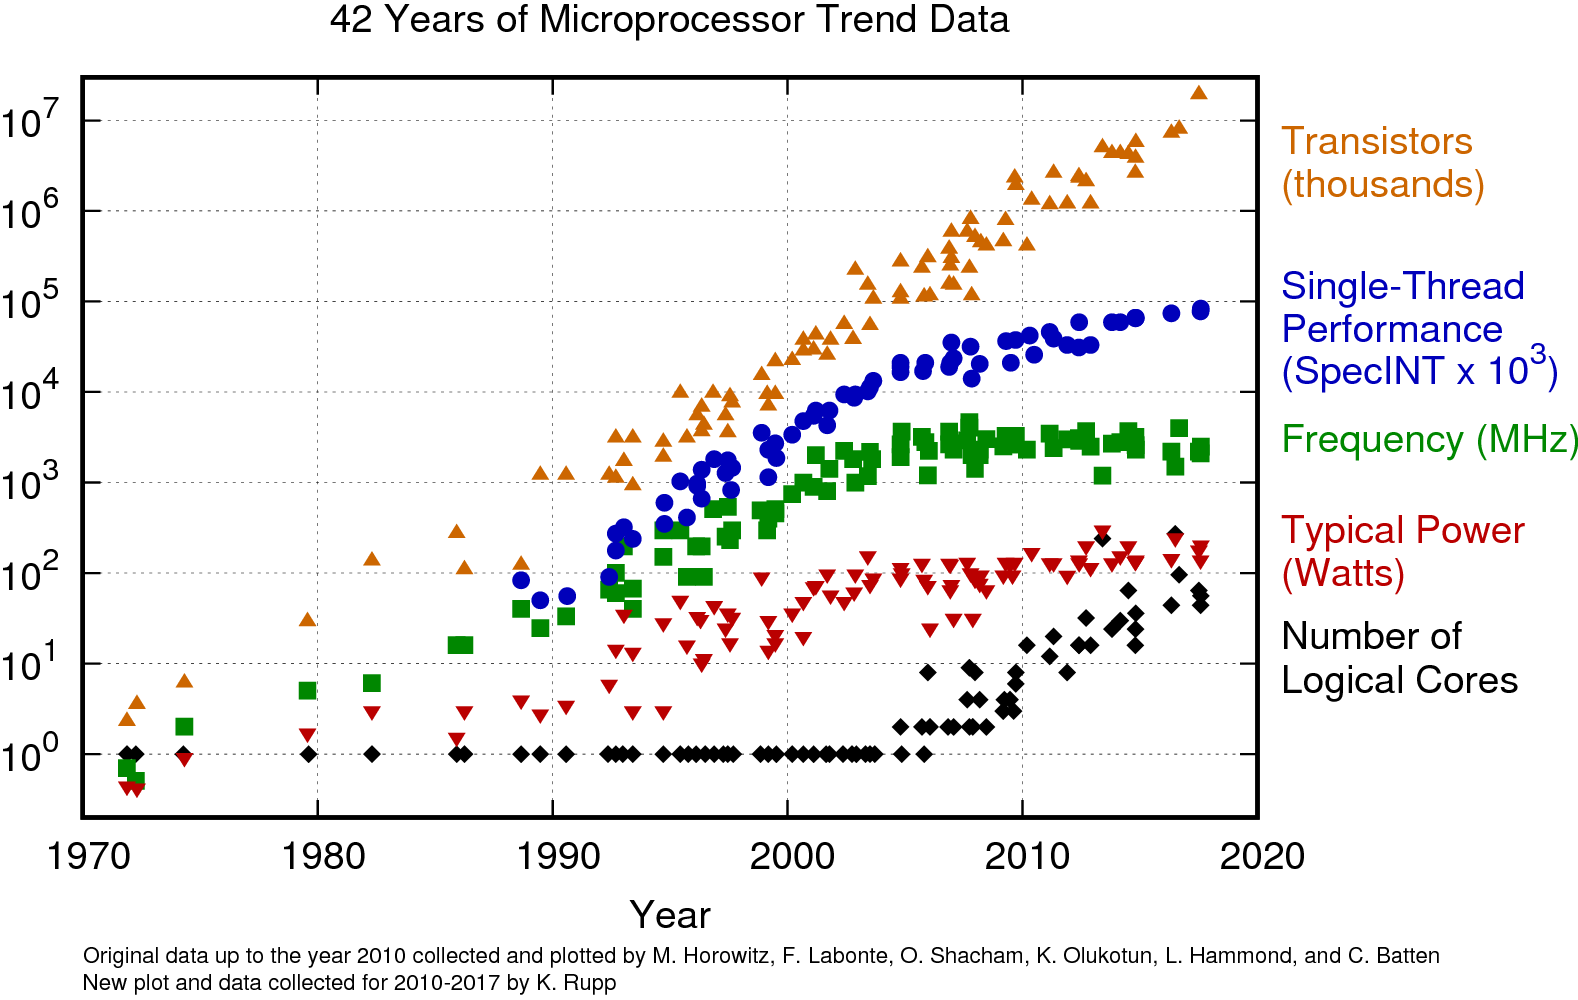
\includegraphics[width=\textwidth]{42-years-processor-trend.png}
  \caption{Le \og \emph{Dennard Scaling} et la loi de Moore illustrées (crédit image : \url{https://www.karlrupp.net})\label{fig:dennard_scaling}.}
\end{figure}

\begin{figure}
  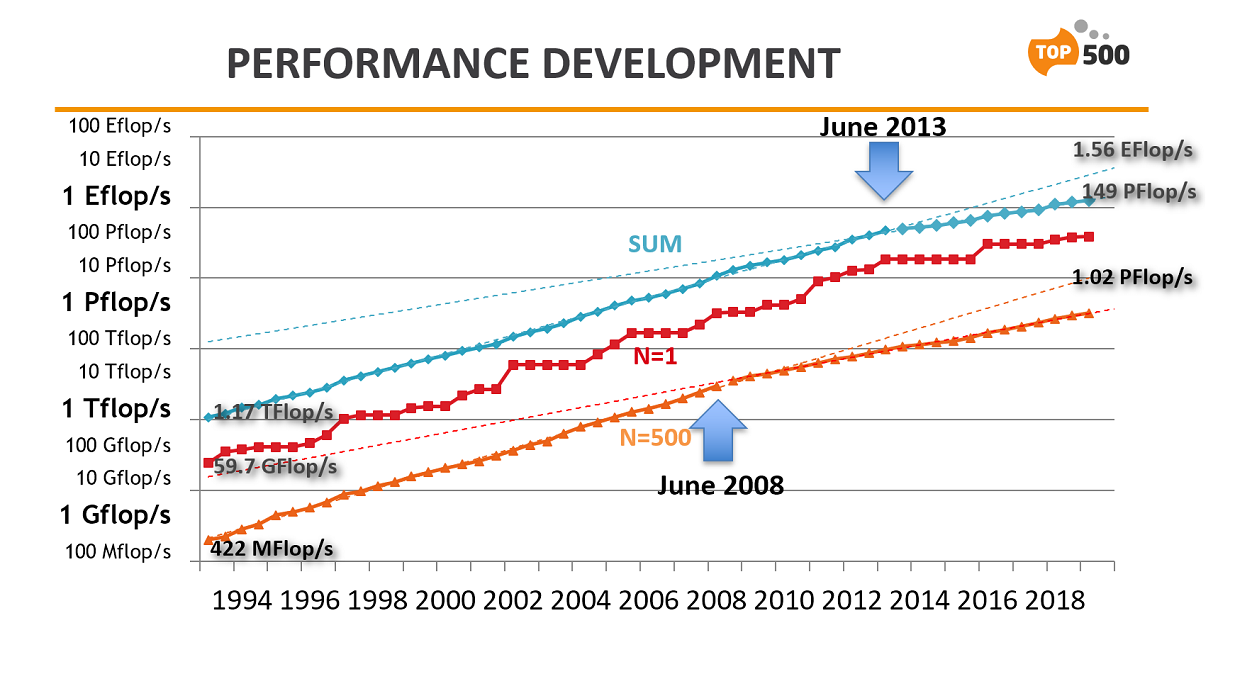
\includegraphics[width=\textwidth]{Top500-Dennard-scaling-effect.png}
  \caption{Répercussion de la fin du \og \emph{Dennard Scaling} sur la puissance
    des ordinateurs du TOP 500. L'effet se fait d'abord sentir sur le 500-ème
    système du classement, avant de se répercuter sur la puissance de calcul
    cumulée des 500 machines.\label{fig:dennard_scaling2}}
\end{figure}

Mais du coup, le parallélisme est une tendance de long terme : les ordinateurs,
et surtout ceux dédiés au calcul scientifique, sont déjà et seront de plus en
plus des machines parallèles, avec beaucoup de coeurs. De nos jours, les
smartphone haut-de-gamme ont déjà 6 ou 8 coeurs.

% \paragraph{Limites physiques} D'ailleurs, malgré des progrès importants, il y a
% des limites à la puissance de calcul que peut posséder \emph{un seul}
% processeur. En effet, à 1Ghz un processeur exécute une instruction en une
% nanoseconde. Si l'on se fie aux idées d'Albert Einstein sur la relativité, la
% vitesse de propagation des signaux électrique est plus petite que la vitesse de
% la lumière, qui est d'environ 30cm par nanoseconde dans le vide, et 20cm/ns dans
% le cuivre ou dans des fibres optiques. À 1Ghz, un processeur doit donc mesurer
% moins de 20cm, sinon ses extrémités seraient \og inaccessibles\fg pendant la
% durée de traitement d'une instruction. À 10Ghz, la limite est donc de 2cm, et à
% 100Ghz, de 2mm. Plus les processeurs seront rapides, plus ils devront être
% petits ! Et plus ils sont petits, plus le problème d'évacuer la chaleur qu'ils
% produisent devient délicat.

\paragraph{Limites énergétiques} La consommation énergétique des ordinateurs
prend de plus en plus d'importance. On estime que les prochains ordinateurs \og
exascale\fg consommeront environ 20MW voire plus. L'évacuation de la chaleur
produite par unités de calcul est un problème majeur de leur conception. Les
processeurs modernes ont beaucoup de coeurs, mais ils ne peuvent pas les faire
tous fonctionner à la fréquence maximale sous peine de surchauffe.

\begin{danger}
  Sur les processeurs Intel les plus communs, cette caractéristique porte le
  nom commercial de \og \textit{turbo boost}\fg. L'idée c'est que lorsqu'un seul
  coeur est utilisé, il peut être \og overclocké\fg, mais lorsque tous les
  coeurs sont utilisés, c'est impossible. Par exemple, les processeurs Intel
  Xeon Gold 6248 qui équipent le calculateur \og Jean-Zay\fg du CNRS ont 20
  coeurs. Chaque coeur est capable de fonctionner à 3.9Ghz ! Mais tous ensemble,
  ils sont limités 2.5Ghz (la dissipation de chaleur serait trop importante
  s'ils étaient tous à fond).
\end{danger}

\begin{ddanger}
  En réalité, c'est encore plus compliqué que ça. Sur les processeurs Intel \og
  Skylake\fg et suivants, la fréquence maximale d'une part et \og minimum
  garantie\fg d'autre part dépendent de la nature des calculs effectués : s'ils
  sont scalaires (fréquence la plus élevée), riches en AVX2 (fréquence moins
  élevée) ou riches en AVX-512 (encore moins élevée).
\end{ddanger}


Dans le HPC, la prise en compte de la consommation énergétique des calculs est
principalement le problème des ingénieurs qui conçoivent les composants
matériels. Vu de loin, la répercussion de ces contraintes sur les applications
parallèle est à peu près la suivante : il est plus efficace, énergiquement
parlant, d'avoir beaucoup de processeurs simples et lents, plutôt que peu de processeurs
complexes et rapides. Or ceci nécessite de faire des calculs largement parallèles.

En effet, il découle des raisonnements ci-dessus que si on veut augmenter la
fréquence, il faut que les conducteurs se chargent plus vite. Pour cela, il faut
augmenter l'intensité des courants. Et pour cela, il faut augmenter la
tension. Du coup, la puissance dynamique dissipée, qui est asymptotiquement
$V^2f$, est en fait en $f^3$. On a tout intérêt à garder $f$ assez faible pour
minimiser la puissance.

Par exemple, dans~\cite{LeeWACSSA14}, les promoteurs de l'architecture libre
\texttt{RISC-V} démontrent un processeur capable d'aller jusqu'à 1.3Ghz, mais
dont l'efficacité énergétique est maximale à 250Mhz : la puce réalise alors 16.7
GFlops/W. Pour aller dans le même sens, dans l'article~\cite{VogeleerMJC13}, les
auteurs exécutent un petit code de calcul sur un processeur de smartphone. Il
s'agit d'un code qui permute de manière déterministe les éléments d'un tableau,
et qui est notamment utilisé dans le calcul de la transformée de Fourier rapide
(FFT). Les auteurs observent que la consommation d'énergie divisée par la taille
du tableau a un optimum (vers 600-700MHz) qui n'est pas la fréquence maximale
(de 1.6Ghz) (cf. fig~\ref{fig:freq_scaling}).

\begin{figure}
  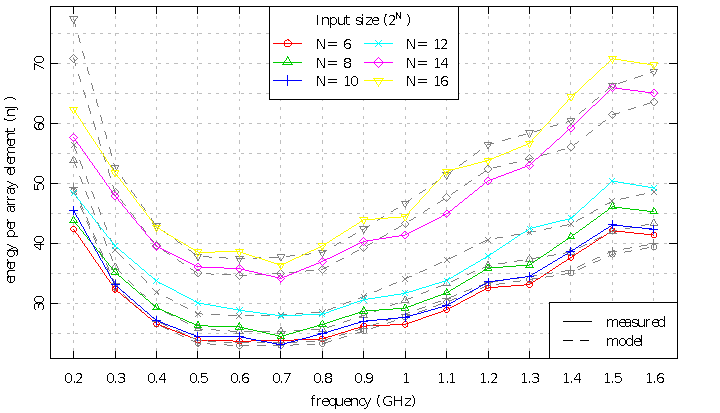
\includegraphics[width=\textwidth]{cpu_freq_scaling.pdf}
  \caption{Efficacité énergétique d'un calcul (en nJ par élément traité) en
    fonction de la fréquence d'horloge du CPU. L'optimum énergétique est atteint
    pour une fréquence donnée, qui n'est ni la minimale, ni la maximale. Le CPU
    est un processeur de smartphone (Cortex-A9) (image
    :~\cite{VogeleerMJC13}). \label{fig:freq_scaling}}
\end{figure}

Autre exemple : l'ordinateur massivement parallèle IBM BlueGene/Q. Les
ingénieurs d'IBM ont conçu une machine massivement parallèle en assemblant un
grand nombre de processeurs \og lents\fg. Ils ont pris un processeur simple
(RISC, \emph{in-order}, le PowerPC A2), et ils ont délibérément choisi de faire
le fonctionner à 1.6Ghz alors qu'il aurait supporté 2.4Ghz : ce choix améliore
l'efficacité énergétique. Avec 98304 tels processeurs (à 16 coeurs), ils ont
obtenu simultanément la meilleure place au Top500 (17.1 PFLOPS en 2011) et au
Green500 (2.1 GFLOPS/W pour l'ensemble de la machine).

Aujourd'hui, les microprocesseurs \og normaux\fg sont gros (beaucoup de
transistors), rapides (fréquence élevée), complexes, avec beaucoup de
parallélisme à l'intérieur pour masquer les latences (\emph{out-of-order}),
etc. À l'avenir, les contraintes énergétiques seront plus dures. Une stratégie
possible consiste à utiliser des processeurs petits, simples, plus lents, avec
peu de parallélisme à l'intérieur (\emph{in-order}). C'est d'ailleurs
\emph{déjà} largement ce qui se passe à l'intérieur des \og accélérateurs\fg de
calculs de type GPU, Xéon Phi et autres \emph{many-cores}. C'est notamment pour
cette raison qu'ils sont plus efficaces d'un point de vue énergétique (plus de
calculs réalisés par Joule dissipé).

On y reviendra plus tard, mais il se trouve que les programmeurs peuvent jouer
un rôle dans l'amélioration de la consommation énergétique : le moyen le plus
sûr d'écrire des programmes économes en énergie consiste à écrire des
programmes...  \og haute-performances\fg.

\section{Le HPC a de beaux jours devant lui}

(cette section n'est pas rédigée)

Quasiment tous les domaines du calcul scientifique sont désormais concernés.

Pour ne donner qu'un exemple en géophysique (recherche de gisements pétroliers
en vue de futurs forages)~: d'après des représentants de Total (en 2018) : le
coût d'un forage en eau peu profonde est de $\approx \$30$ millions. Le coût
d'un forage en eau profonde est de $\approx \$100$ Millions. Mieux vaut investir
dans une machine de calcul scientifique et faire des simulations que de rater un
forage !

Autres domaines problématiques : simulation d'écoulements turbulents (par
exemple les combustions), simulation de l'interaction entre des molécules
complexes (protéines) en simulant les forces élémentaires entre les atomes, etc.

Voir aussi les grands challenge scientifiques (d'après Quinn) :
Levin. E. ''Grand challenges to computational science." Communications of the
ACM 32(12): 1456-1457, December 1989.

\section{Qu'est-ce qu'une machine dédiée au HPC ?}

On peut bien sûr faire de la programmation parallèle et viser un bon niveau de
performance sur des ordinateurs \og normaux\fg, ou bien avec la \og machine
parallèle du pauvre\fg (des PCs de bureau reliés par un réseau ethernet
classique). Mais les machines dédiées au calcul scientifique sont aux
ordinateurs normaux ce qu'une Formule 1 est à une petite citadine. Les
processeurs n'ont rien à voir, le réseau n'a rien à voir et le stockage n'a rien
à voir.

Tout d'abord, voici un petit glossaire :
\begin{description}
\item[machine] l'ensemble des composants : \emph{noeuds} de calcul, réseau,
  stockage, etc.
  
\item[noeud (\textit{node})] un \og ordinateur\fg indépendant (dans le cadre
  d'une machine parallèle qui en contient plusieurs), constitué d'un ou
  plusieurs processeurs, d'une mémoire et d'une interface le connectant au
  réseau.

\item[baie (\textit{rack})] une armoire destinée à recevoir des boîtiers,
  typiquement les noeuds, des commutateurs réseaux, des modules d'alimentation
  électriques, etc. Leur taille est souvent standardisée : 46.5 cm de large (19
  pouces) et 1.8m de haut.

\item[multiprocesseur (\textit{Symmetric Multi Processing} / SMP)] se dit d'un
  noeud qui contient plusieurs processeurs qui ont accès à la même mémoire.

\item[processeur (\textit{CPU})] un circuit intégré qui constitue un objet
  unique physique. Il contient au moins un \emph{coeur} (cf. ci-dessous), ainsi
  que potentiellement du cache, des contrôleurs mémoire, éventuellement des
  interfaces à d'autres périphériques (réseau, PCI express, etc.).
  
\item[coeur (\textit{core})] un ensemble de circuits capables d'exécuter du code
  de façon autonome. En particulier, un coeur contient en principe une unité
  arithmétique (ALU), une unité de gestion de la mémoire (MMU), bien souvent un
  cache de données/d'instructions, ainsi qu'au moins un \emph{thread matériel}
  (cf. ci-dessous).

\item[multicoeur] se dit d'un processeur qui contient plusieurs coeurs.
  
\item[thread matériel (\textit{hardware thread})] un contexte d'exécution
  autonome à l'intérieur d'un coeur. Constitué au moins d'un banc de registres
  (\textit{register file}) et un pointeur d'instruction, etc. Parfois appelé \og
  coeur logique\fg.

\item[\textit{Simultaneous Multi-Threading}] se dit d'un coeur qui héberge
  plusieurs threads matériels. Les unités d'exécution (arithmétique et logique,
  flottante, mémoire, cache éventuel, etc.) sont \emph{mutualisées} entre les
  threads. L'intérêt de cette technique est que si l'un des threads est bloqué,
  les autres peuvent continuer à exploiter le matériel.
\end{description}

\begin{danger}Il est très facile de confondre
  processeur/coeur/thread. Grosso-modo : un processeur est un objet (qui
  s'insère dans un \og \emph{socket}\fg) qui contient au moins un coeurs (ainsi
  que d'autres bricoles) ; un coeur héberge au moins un thread matériel. Pour
  fixer les idées, la figure~\ref{fig:arch1-bis} contient deux exemples. Depuis le
  milieu des années 2000, les processeurs les plus communs ont deux threads
  matériel par coeur (chez Intel, ceci porte la dénomination commerciale \og
  HyperThreading\fg). Certains processeurs peuvent en avoir plus.
\end{danger}

On dit parfois \og processeur\fg par abus de langage, pour dire \og coeur\fg ou
\og unité de traitement\fg. Au CNRS, les \og CPU-hours\fg désignent le nombre
d'heure de calcul multiplié par le nombre de coeurs utilisés. Sur le cloud
Amazon, un vCPU est un thread matériel, etc. Ce qui complique les choses, c'est
que sous la plupart des systèmes d'exploitations, les threads matériels
apparaissent comme des processeurs indépendants.


\begin{danger}
  Il est aussi très facile de confondre thread matériel/thread logiciel. Un
  thread logiciel est un contexte d'exécution au sein du système
  d'exploitation. L'ordonnanceur de l'OS place les threads logiciels sur les
  threads matériels disponibles\footnote{la surcharge du mot \og thread\fg est
    pénible.}. En général, dans un OS moderne, des dizaines de
  processus/threads logiciels s'exécutent de manière concurrente, et
  l'ordonnanceur de l'OS choisit lesquels affecter aux (quelques) threads
  matériels pendant le prochain quantum de temps. Des changements de contexte
  périodiques et suffisamment rapides peuvent donner l'illusion à l'utilisateur
  d'une exécution simultanée de tous ces processus.
\end{danger}

\begin{figure}[htpb]
      \centering
  \begin{subfigure}[t]{0.4\textwidth}
    \centering
    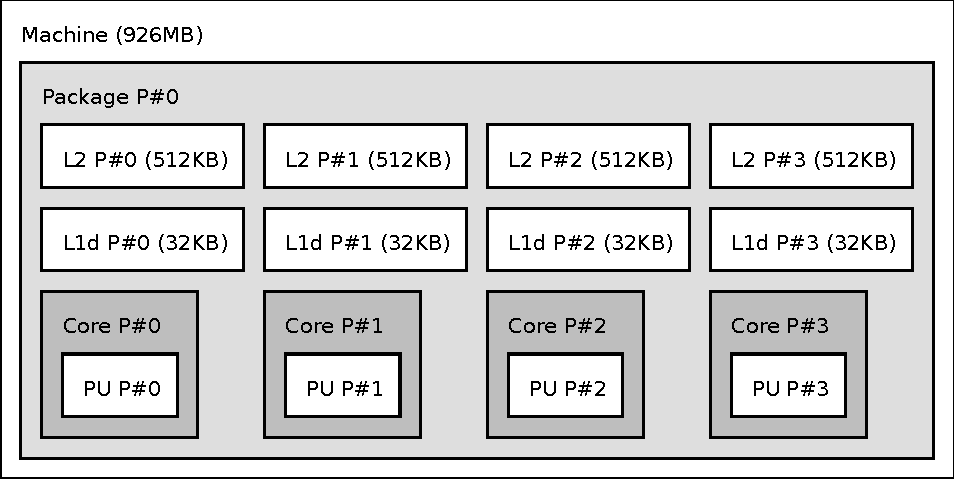
\includegraphics[width=\textwidth]{lstopo_rpi3b.pdf}
    \caption{Un processeur (ARM Cortex A53), quatre coeurs. Chaque coeur possède
      32Ko de cache L1 et 512Ko de cache L2.}
  \end{subfigure}
  \hspace{5mm}
  \begin{subfigure}[t]{0.4\textwidth}
        \centering
    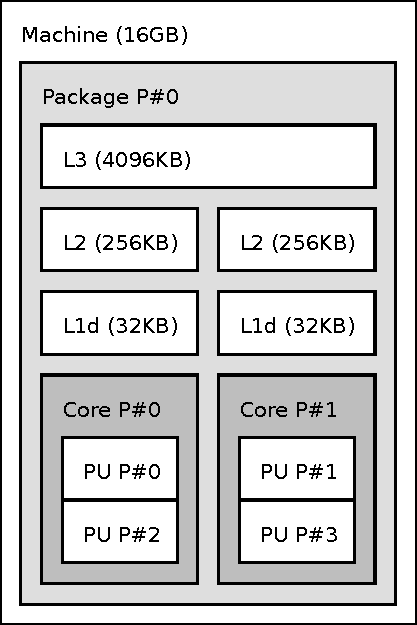
\includegraphics[width=3cm]{lstopo_laptop.pdf}
    \caption{Un processeur (Intel Core i7 6600U), deux coeurs, deux threads
      matériels par coeur. Chaque coeur possède 32Ko de cache L1 partagé entre
      les deux threads ainsi que 256Ko de cache L2. Le processeur contient un
      cache L3 de 4Mo partagé entre les deux coeurs.}
  \end{subfigure}
  \caption{À Gauche, un Raspberry Pi modèle \texttt{3B+}. À droite, le laptop du prof. \label{fig:arch1-bis}}
\end{figure}

\begin{itemize}
\item Le CNRS possédait, de 2011 à 2019 une machine IBM Bluegene/Q. C'est une
  \og petite\fg installation avec seulement 6 rack. Chaque rack contient 1024
  noeuds, chaque noeud contient un processeur PowerPC A2 à 16 coeurs et 16Go de
  RAM, cadencé à 1.6Ghz (cf. fig.~\ref{fig:powerpcA2}). Il y a donc 98~304 coeurs
  en tout et 98To de RAM. La puissance de crête est 1.2 PetaFLOPS et la machine
  consomme 600kW. Chaque processeur contient une interface réseau \og maison\fg
  avec 10 liens à 2Go/s dans chaque sens vers 10 autres processeurs (tore
  5D). Chaque coeur héberge de 1 à 4 threads matériel (au choix du
  programmeur). Refroidissement par eau. Les noeuds exécutent une version
  \emph{light} de Linux (les utilisateurs ne peuvent pas se connecter aux
  noeuds). Coût : $\approx 20$ millions d'euros.

\medskip
  
\item Le 12ème ordinateur le plus puissant du monde, \texttt{sequoia}, est une
  BlueGene/Q de 96 racks, donc 1 572 864 coeurs, 1.5Po de RAM et 10MW de
  consommation électrique.

  \medskip
  
\item Le CNRS vient (en 2019) de faire l'acquisition d'une machine plus moderne
  (\texttt{jean-zay}) construite par HPE. Il est composé de 1528 noeuds \og
  scalaires\fg contenant 2 processeurs (Intel Xeon \og Cascade Lake\fg 6248) à
  20 coeurs, 2.5Ghz et 192Go de RAM. Il y a aussi 261 noeuds \og convergés\fg
  qui contiennent aussi 4 GPU NVIDIA V100 SXM2 avec 32Go de RAM chacun. Il y a donc
  61 120 coeurs CPU, 1044 GPUs et 343To de RAM en tout. La puissance de crête
  est 14 PetaFLOPS. Refroidissement par eau chaude. Réseau Intel OmniPath
  100Gb/s.

\medskip
  
\item À l'échelle mondiale, la machine la plus puissante est \texttt{summit},
  construite par IBM. Composée de 4608 noeuds avec chacun 2 processeurs Power9 à
  22 coeurs, 6 GPU NVIDIA V100 et 600Go de RAM. Consommation électrique :
  13MW. Coût : $\approx \$500$ millions. Puissance de crête : 200
  PetaFLOPS. Réseau Infiniband 100Gb/s. Total: 202 752 coeurs, 27 648 GPUs,
  2.7Po de RAM.

\medskip
  
\item En position numéro 5, on trouve \texttt{Frontera}, construit par Dell, la
  machine la plus puissante installée dans une université. Composée de 8008
  noeuds, chacun avec 2 processeurs (Intel Xeon platinum 8280 \og Cascade
  Lake\fg, cf. fig.~\ref{fig:grosXeon}) à 28 coeurs, 2.7Ghz et 192Go de
  RAM. Réseau Infiniband 100Gb/s. Puissance de crête : 39 PetaFLOPS. Total :
  448~448 coeurs et 1.5Po de RAM. Coût : $\approx \$60$ millions.

\medskip
  
\item En cours de construction, mais qui va bientôt dominer le classement,
  \texttt{fugaku} construit par Fujitsu. Composée de 150 000+ noeuds, chacun
  avec un processeurs (Fujitsu A64FX, cf. fig.~\ref{fig:A64FX}) à 48 coeurs,
  2Ghz et 32Go de RAM HBM (très rapide). Réseau maison \og Tofu 3\fg (tore 3D de
  tore 3D). Puissance de crête : 400+ PetaFLOPS. Total : 7 200 000+ coeurs et
  4.7Po de RAM. $\approx 900$ millions d'euros.

\medskip
  
\item Et bien sûr, la machine parallèle du pauvre : les 16 PCs à 4 coeurs d'une
  salle de TP reliés par un switch Gigabit ethernet (dans le meilleur des cas).
\end{itemize}

\begin{figure}
  \centering
  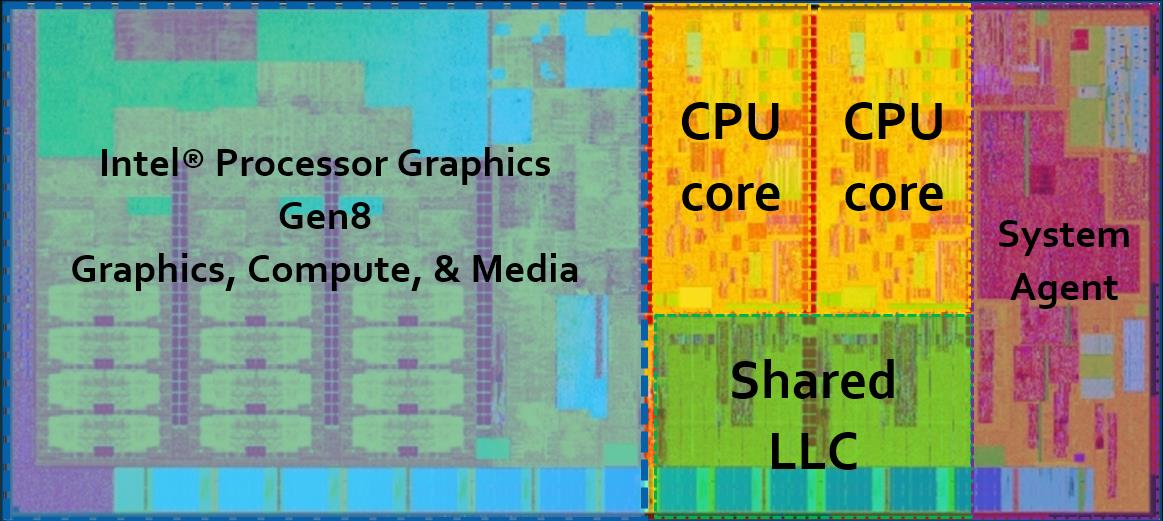
\includegraphics[width=8cm]{i5-silicon-die-layout.jpg}
  \caption{Un processeur contemporain (Intel core i5 \og Skylake\fg) à deux
    coeurs habituel dans les laptops. 3Mo de cache et GPU intégré. (image : Intel)}
\end{figure}

\begin{figure}
  \centering
  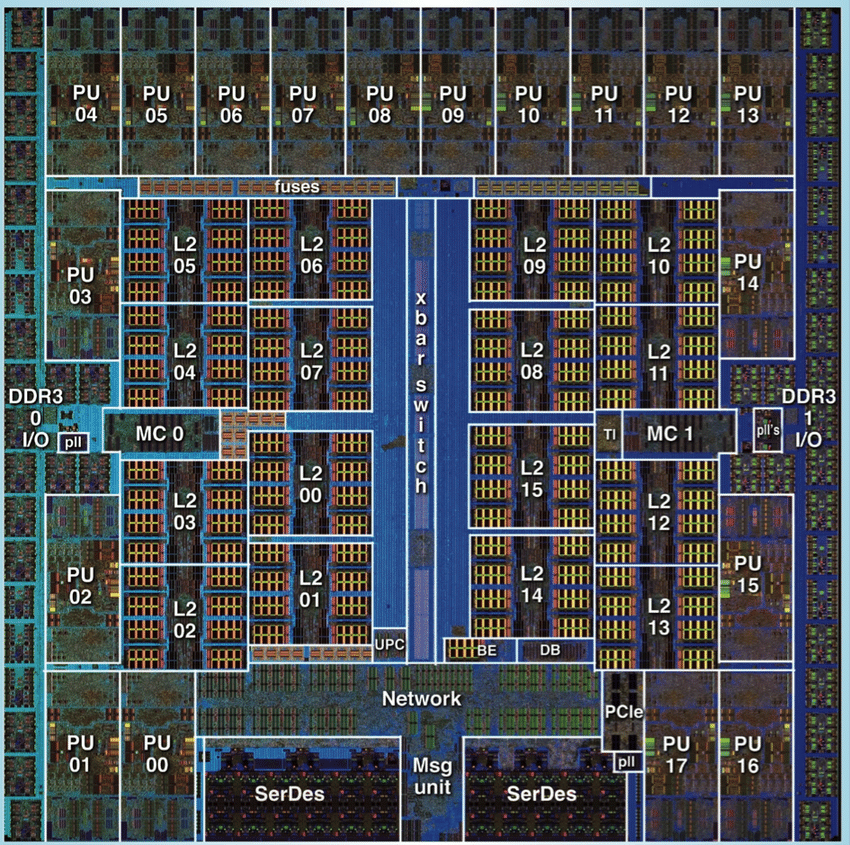
\includegraphics[width=8cm]{die-bgq.png}
  \caption{Un processeur PowerPC A2 de 2011--2012, utilisé dans les machines IBM
    Bluegene/Q. 18 Coeurs (16 pour les applications, 1 réservé pour l'OS, 1
    spare), 32Mo de cache, 2 contrôleurs mémoire DDR3 et 11 contrôleurs réseau
    2Go/s intégrés. (image : IBM) \label{fig:powerpcA2}}
\end{figure}

\begin{figure}
  \centering
  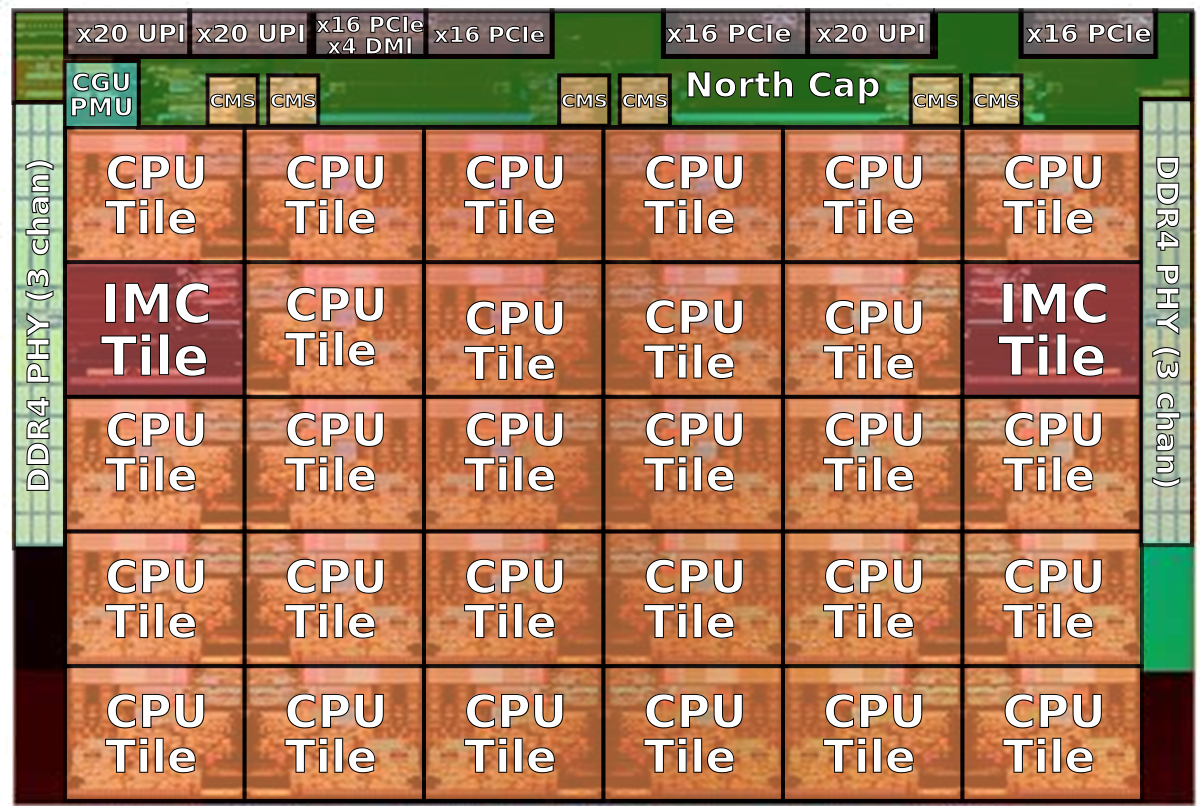
\includegraphics[width=10cm]{skylake-sp_xcc_die_shot.png}
  \caption{Un processeur Intel Xeon \og Skylake\fg de 2019 à 28
    coeurs. Contrôleur réseau (OmniPath) et 6 contrôleurs mémoire DDR4
    intégrés. (image : Intel) \label{fig:grosXeon}}
\end{figure}

\begin{figure}
  \centering
  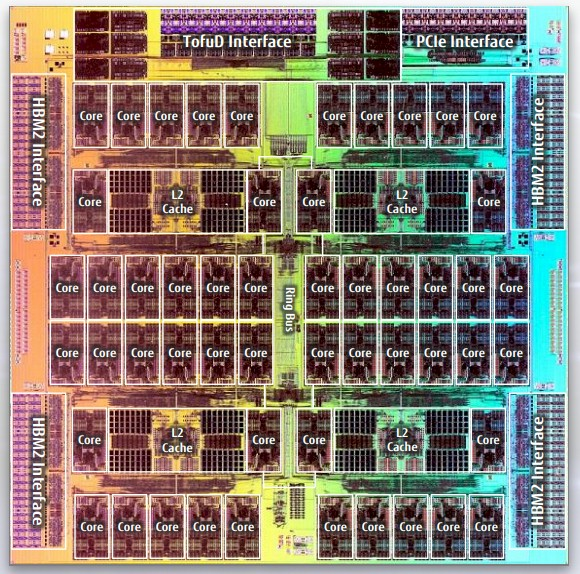
\includegraphics[width=10cm]{fujitsu-a64fx-block-diagram.jpg}
  \caption{Un processeur A64FX de 2019 (jeu d'instruction ARM) conçu par Fujitsu
    pour la machine \og Fugaku\fg. 52 coeurs (48 pour les applications, 4 pour
    l'OS), 32Mo de cache, contrôleur réseau (TofuD) et contrôleur mémoire HBM2
    intégré. (image : Fujitsu)~\label{fig:A64FX}}
\end{figure}

\subsection{Petit historique}

%Et avant ?

(cette section est incomplète)

En 1997, Intel livre l'ASCII red, avec plus de 9000 processeurs Pentium
Pro. C'est la première machine à atteindre 1 TeraFLOPS.

En 2008, \texttt{road runner} conçu par IBM atteint 1 PetaFLOPS. Composé de 296
racks, il contient 12~960 processeurs IBM PowerXCell 8i (contenant 1 gros coeur
Power PC et 8 mini-coeurs) et 6~480 AMD Opteron à deux coeurs. Coût :
$\approx \$100$ millions.

En 2011, le \texttt{K computer} japonais atteint 10 PetaFLOPS. Il contient
88~128 processeurs SPARC64 VIIIfx à 2Ghz et 8 coeurs, répartis dans 864 racks
(ça fait 705~024 coeurs).

\section{Architectures parallèles}

Les sections précédentes démontrent qu'il existe une grande variabilité dans
l'architecture des machines parallèles. Différents niveaux de parallélisme
existent : à l'échelle de la machine (plusieurs noeuds), à l'intérieur d'un
noeud (plusieurs processeurs), à l'intérieur d'un processeur (plusieurs coeurs),
à l'intérieur d'un coeur (plusieurs threads et/ou plusieurs unités d'exécutions).

Pour chaque niveau, il convient de savoir combien d'éléments de calcul sont
présent ?  Quelle est leur puissance ? Sont-ils homogènes ? De quelle mémoire
disposent-ils ? Comment sont-ils reliés les uns aux autres ? Comment
synchronisent-ils leurs efforts ?

\subsubsection{Classification de Flynn} En 1966, Michal J. Flynn (1934--) a proposé
une classification des architectures parallèles qui est restée
depuis. Grosso-modo, il s'agit de distinguer le parallélisme de contrôle d'une
part (SI = Single Instruction / MI = Multiple Instruction) d'une part, et le
parallélisme de données d'autre part (SD = Single Data / MD = Multiple Data).

\begin{center}
\begin{tabular}{|l|l|c|c|}
\cline{3-4}
\multicolumn{2}{c|}{}    & \multicolumn{2}{c|}{Flot de données} \\
\cline{3-4}
\multicolumn{2}{c|}{}    & unique & multiple \\
\hline
Flot           & unique   & SISD   & SIMD \\
\cline{2-4}
d'instructions & multiple & MISD   & MIMD \\
\hline
\end{tabular}
\end{center}

Les architectures SISD sont \og purement séquentielles\fg : un processeur
exécute un flot d'instruction, et chaque instruction opère sur une seule donnée.

Dans les architectures SIMD, les unités de traitement (\og \textit{Processing
  Units}\fg, PU) exécutent simultanément la même opération sur des données
différentes. Par exemple, la même instruction effectue plusieurs (2, 4, 8, 16,
...) additions flottantes simultanément sur des \og vecteurs\fg. Ceci est en
fait très répandu : un GPU haut-de gamme (style NVIDIA V100) contient 80 \og
coeurs\fg, qui sont en fait de grosses unités SIMD capable de traiter 32
\texttt{double} / 64 \texttt{float} simultanément. Les processeurs habituels
contiennent aussi des unités SIMD : instructions SSE (128 bits, $4 \times$
\texttt{float}, puis AVX2 (256 bits, $8 \times$ \texttt{float}) et maintenant
AVX-512 ($16 \times$ \texttt{float}). Les processeurs de smartphone ont aussi
des instructions SIMD NEON (128 bits, $4 \times$ \texttt{float}). Tout ceci
avait été précédé par des machines dites \og vectorielles\fg (CRAY, NEC) qui
dominaient le monde du HPC dans les années 1970--1990 : les processeurs
pouvaient traiter des vecteurs entiers en une seule instruction. Après être un
peu tombé en désuétude, cela revient à la mode !

Les architectures MISD (plusieurs instructions différentes appliquées aux mêmes
données) sont assez rare, surtout sous cette forme pure. Mais les
\textit{systolic arrays} peuvent être vu de la sorte.

Les architectures MIMD sont très courantes : des processeurs indépendants
peuvent effectuer différentes opérations sur différentes données
simultanément. Ils ont un fonctionnement asynchrone (chaque processeur est
autonome et gère son propre flux de donnée). Par exemple : les processeurs
multicoeur, un cluster de PC, etc.

Quand on se pose la question en terme de \og technique de programmation\fg, on
est amené à envisager les différents types de systèmes en deux grandes
catégories :
\begin{description}
\item[machines à mémoire partagée] \hfill\\
  Les différents unités de traitement ont accès à la même mémoire (elles sont
  probablement connectées à un même bus, et sont synchronisées). Un seul système
  d'exploitation fonctionne sur l'ensemble des processeurs, alloue la RAM, etc.

  Les différents processus d'une même application parallèle possèdent un espace
  mémoire commun, des variables globales. Ceci leur permet (ou leur évite, selon
  le point de vue) de communiquer explicitement.

\item[machines à mémoire distribuée] \hfill\\
  Les unités de traitement possèdent chacune leur propre mémoire séparée, et
  exécutent probablement chacune leur propre système d'exploitation.

  Le seul moyen de communication disponible est le réseau. Il est géré en partie
  par l'OS (UDP, TCP/IP, etc.) et en partie par des librairies qui appartiennent à
  l'utilisateur (\textit{middleware}). La synchronisation, l'accès aux
  ressources, la répartition de la charge, ne sont pas gérées par l'OS et
  doivent être assurées par l'application parallèle.
\end{description}

\subsubsection{Machines à mémoire partagée}

Par bien des aspects, les machines à mémoire partagée sont plus faciles à
programmer. Pas besoin de s'embêter avec une gestion du réseau, des adresses IP,
des liens réseaux qui tombent en panne, des machines qui ne vont pas toutes à la
même vitesse, qui ne sont pas toutes à l'heure (!), etc.

Par contre, si plusieurs processeurs ont accès à la même mémoire, cela ouvre la
porte à des conflits d'accès (\textit{race conditions}) : lorsqu'au moins deux
processeurs tentent d'accéder simultanément à la même adresse mémoire et qu'au
moins un de ces accès est une écriture, le résultat est mal défini.  Afin
d'éviter ces conflits, la synchronisation entre les différents processus doit
est assurée par des mécanismes explicites, typiquement des verrous ou des
sections critiques qui sont en partie gérés par l'OS.

L'inconvénient des machines à mémoire partagée, c'est qu'il est difficile de les
faire grossir au-delà d'une certaine limite (la plus grosse dont j'ai entendu
parler, une \marque{Silicon Graphics Altix UV}, aurait 2048 processeurs ---
c'est-à-dire rien du tout face aux dizaine/centaines de milliers de processeurs
des plus grosses machine de HPC). En effet, tous les processeurs sont \og en
compétition\fg pour l'accès aux données en RAM.

\begin{danger}
  Pourquoi les machines à mémoire partagée ne passent pas à l'échelle ? L'accès
  des processeurs à la RAM fonctionne \textit{grosso modo} de la façon
  suivante. Le processeur est relié au contrôleur de la RAM par un
  bus. Lorsqu'il veut accéder au contenu d'une adresse spécifique en RAM, le
  processeur écrit l'adresse requise sur le bus, et envoie un \og ping\fg au
  contrôleur sur le bus. Le contrôleur lit l'adresse, récupère le contenu, écrit
  ensuite la valeur lue en RAM sur le bus, et envoie un signal \og pong\fg sur
  le bus. A la réception du signal, le processeur lit la valeur sur le bus.

  Si toute la RAM et tous les processeurs sont reliés au même bus, alors seul un
  processeur peut utiliser le bus à chaque instant, et tous les autres doivent
  attendre qu'il ait fini. Plus le nombre de processeur est élevé, et plus le
  temps d'attente pour la RAM augmente. Cette technique est donc limitée à un
  petit nombre de processeurs (typiquement de 2 à 4).
\end{danger}


\paragraph{Archuitecture NUMA} Une autre solution consiste à relier directement
chaque processeur à une petite partie de la RAM, par un bus qui lui est
propre. Cette partie de la RAM est alors entièrement sous son contrôle. Pour
accéder au reste de la RAM, il doit en \og négocier\fg l'accès avec les autres
processeurs, via des bus ou des connexions directes. L'accès au reste de la RAM
est alors plus lent que l'accès à sa \og région propre\fg. Cette architecture
est appelée \og \textit{Non-Uniform Memory Access} (NUMA)\fg. Elle est très
répandue actuellement (un des avantages est que le contrôleur mémoire peut être
incorporé au processeur, rendant la communication très
rapide). Cf. fig.~\ref{fig:chiclet}. Mais en fait, si on regarde ça de loin, on
se rend compte que les architectures NUMA sont un moyen de \emph{simuler une
  machine à mémoire partagée avec une machine à mémoire distribuée} (et un
réseau très, très rapide).

Pour de bonnes performances, il est alors critique que l'OS soit conscient de la
topologie de cette hiérarchie mémoire, qu'il ne déplace pas un processus d'un
CPU à l'autre (sinon le processus se trouve éloigné de \og ses\fg données), et
qu'il alloue de mémoire de manière judicieuse (ne pas donner à un processus de
la mémoire \og lointaine\fg). Cela pose des problèmes d'ordonnancement des
tâches plus compliqués. Certains algorithmes peuvent être optimisés pour ces
architectures. Mais de toute façon, la \emph{localité} des accès mémoire est un
aspect important du HPC, mémoire uniforme ou pas.

En \the\year, un noeud SMP est quasi-systématiquement de type NUMA.

\begin{danger}
  Partager la mémoire entre plusieurs processeurs pose des problèmes assez
  compliqués au niveau du matériel, notamment car il faut plus ou moins
  synchroniser leurs caches : si le processeur $A$ modifie ce qui se trouve à
  une certaine adresse en mémoire, et que ces données étaient répliquées dans le
  cache du processeur $B$, alors il faut que $B$ mette à jour (ou invalide) son
  cache --- mais pour ça il faut qu'il soit conscient de l'écriture du
  processeur $A$ !

  Si un bus mémoire est partagé, alors les uns et les autres peuvent \og
  espionner\fg les écritures qui ont lieu sur le bus et invalider
  automatiquement leur cache. Mais dans les machines NUMA, c'est plus
  compliqué~! Il faut que les processeurs communiquent pour s'informer de leurs
  écritures mutuelles dans certains cas.
\end{danger}

\begin{figure}
  \centering
  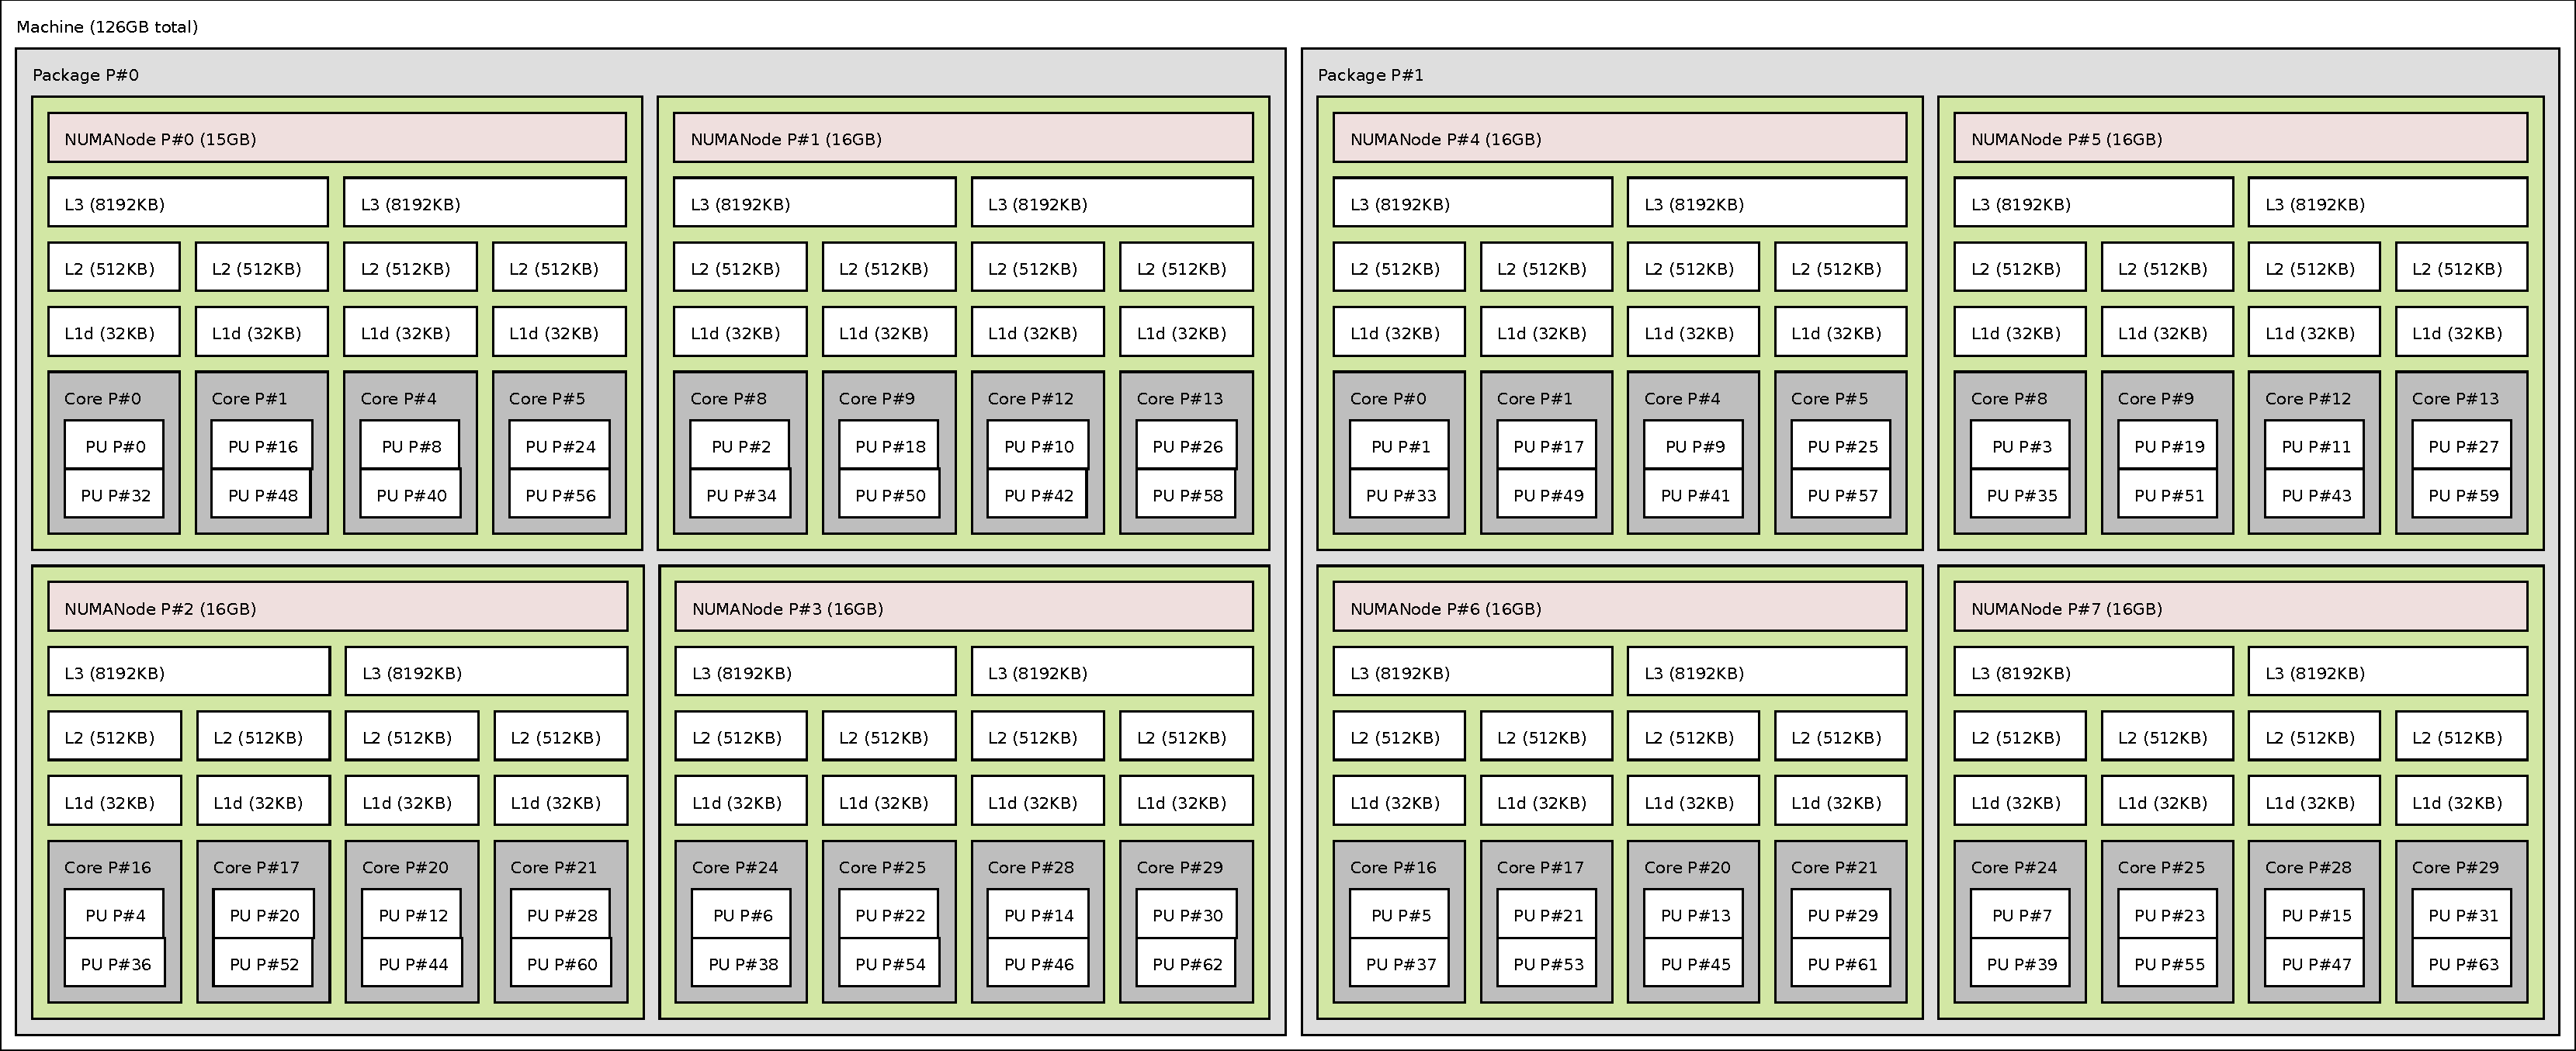
\includegraphics[width=\textwidth]{lstopo_chiclet}
  \caption{Un noeud (du cluster chiclet de GRID5000) contenant deux processeurs
    AMD EPYC 7301. Chaque processeur contient quatre \og paquets\fg de quatre
    coeurs adossés à un contrôleurs mémoire indépendant, connecté à une partie
    des barrettes de RAM. Chaque processeur contient 4 \og zones NUMA\fg et
    l'ensemble de la machine en contient 8. Ci-dessous, la matrice des \og
    distances\fg entre zones NUMA (plus la distance est grande, plus l'accès est
    lent). \label{fig:chiclet}}

\medskip
  
\begin{tabular}{|c||c|c|c|c|c|c|c|c|}  
  \hline
  node &  0 &  1 &  2 &  3 &  4 &  5 &  6 &  7 \\
  \hline\hline
  0 &  10 & 16 & 16 & 16 & 28 & 28 & 22 & 28 \\
  \hline
  1 &  16 & 10 & 16 & 16 & 28 & 28 & 28 & 22 \\
    \hline
  2 &  16 & 16 & 10 & 16 & 22 & 28 & 28 & 28 \\
    \hline
  3 &  16 & 16 & 16 & 10 & 28 & 22 & 28 & 28 \\
    \hline
  4 &  28 & 28 & 22 & 28 & 10 & 16 & 16 & 16 \\
    \hline
  5 &  28 & 28 & 28 & 22 & 16 & 10 & 16 & 16 \\
    \hline
  6 &  22 & 28 & 28 & 28 & 16 & 16 & 10 & 16 \\
    \hline
  7 &  28 & 22 & 28 & 28 & 16 & 16 & 16 & 10 \\
  \hline
\end{tabular}
\end{figure}

\subsubsection{Machines à mémoire distribuée}

Dans les machines à mémoire distribuée (toutes les \og grosses\fg machines
parallèles décrites précédemment), le réseau joue un rôle indispensable pour
relier entre eux les différentes unités de traitement, leur permettre de
coopérer et les synchroniser.

Les caractéristiques (débit, latence) et la topologie du réseau jouent donc un
rôle central dans le niveau de performance atteint \textit{in fine} par les
applications parallèle : communiquer prend du temps, or ce temps est un surcoût
qu'il faut réduire au minimum. Les machines de HPC ont des réseaux \og
haut-de-gamme\fg (Infiniband, OmniPath, etc., alors TCP/IP et ethernet sont bons
pour le \og commun des mortels\fg...), avec des débits élevés mais surtout avec
des latences très faibles.

On rencontre des réseaux en arbre (\og fat tree\fg), des hypercubes, des grilles
(ou des tore) à plusieurs dimensions (5 dimensions pour IBM BlueGene/Q, 6
dimensions pour \texttt{K computer} et \texttt{Fugaku}). Avantage du mesh/tore :
pas de point central de congestion. Inconvénient : nécessité d'un protocole de
routage. Sur \texttt{turing}, la BlueGene/Q du CNRS, on fait le test suivant :
4096 noeud envoient chacun $1.8$Mo à chacun des autres noeud (27.5To sont donc
transmis en tout). Temps total : 18.7s, donc le réseau en tore 5D assure le
transport de $\approx 1.5$To/s.

Comme les performances du réseau sont très critiques, sur les machines les plus
sophistiquées les contrôleurs réseaux sont parfois placés directement sur les
processeurs (IBM BlueGene, Fujistu \og K computer\fg et Fugaku, ... Les
processeurs Intel Xeon Platinum ont un contrôleur OmniPath intégré). Les données
partent et arrivent directement des mémoires les plus rapides (les caches), en
\og tâche de fond\fg pendant que le reste des calculs ont lieu.

La programmation de machines à mémoire distribuées se fait principalement par
l'utilisation de bibliothèques de passage de messages (par ex. MPI) ou par
l'utilisation d'extensions des langages (par ex. les \texttt{coarray} de
Fortran) qui masquent une partie de la complexité.

\subsubsection{Parallélisme au niveau des instructions}

Un processeur réputé séquentiel contient en réalité un certain degré de
parallélisme, même si les programmeurs ne peuvent pas le contrôler
directement. Un exécutable (\og binaire\fg), contient une liste (ordonnée)
d'instructions exécutées par le processeurs. Par exemple (en assembleur
PowerPC)~:

\begin{minted}{gas}
	slwi 10,9,3
	add 8,11,10
	lwzx 10,11,10
	lwz 7,4(8)
	or. 10,10,7
	bne 0,.L146
	addi 5,5,8
	stw 3,0(8)
	stw 4,4(8)
	cmplw 7,6,5
	bne 7,.L24
	lwz 9,144(19)
	li 10,1
	stw 10,20704(31)
	addi 9,9,1
	stw 9,144(19)
\end{minted}

Les processeurs offrent la garantie que tout se passe comme si ces instructions
étaient exécutées les unes à la suite des autres. Mais en fait, pour des raisons
de performance, des formes de parallélisme existent à l'intérieur de ce
processus en apparence séquentiel.

Sans rentrer dans les détails, les processeurs contemporains, même les plus
rudimentaires, ont un \textit{pipeline} (par exemple, le pipeline RISC classique
à 5 étapes : Instruction fetch; Instruction decode; Execute; Memory access;
Writeback. Les processeurs modernes ont parfois des pipelines plus long, avec
10+ étapes). Une instruction met plusieurs cycles à s'exécuter, mais le
processeur peut en \og commencer\fg une à chaque nouveau cycle, et la faire
avancer dans le pipeline. À un instant donné, il peut y avoir plusieurs
instructions \og en vol\fg dans le pipeline, donc plusieurs instructions en
cours d'exécution.

Un processeur est \og scalaire\fg s'il ne peut exécuter qu'une seule instruction
à chaque cycle. Les processeurs \og superscalaires\fg peuvent en exécuter
plusieurs (si elles sont compatibles). Les unités d'exécutions sont alors
parfois répliquées. Le processeur affecte dynamiquement les instructions aux
différentes unités d'exécutions (dont le nombre n'est pas connu à l'avance par
le programmeur et qui varie d'un modèle de processeurs à l'autre), et le tout
est donc portable. Dans le monde de l'informatique grand public, les processeurs
habituels sont superscalaires depuis l'Intel Pentium de 1993.

Par exemple, sur un coeur Intel Skylake il y a 4 ALU (\textit{Arithmetic and
  Logic Unit}) capable d'exécuter les opérations simples sur les entiers : et,
ou, xor, addition, comparaison. Dans l'ensemble, le coeur est capable d'exécuter
jusqu'à 6 $\mu$-instructions par cycle dans le meilleur des cas.

Il peut par ailleurs y avoir plusieurs pipelines. Par exemple, sur le processeur
PowerPC A2 (qu'on trouve dans l'IBM BlueGene/Q), il y a deux pipelines
parallèles : un pour les opérations entières, un pour les flottantes.

Pour obtenir les performances maximales des unités d'exécutions qui sont
présentes dans le processeur, il faut être capable de leur fournir du travail en
permanence, et de les utiliser simultanément (donc de faire des choses en
parallèle), malgré le fait que le flux d'instructions à exécuter soit \og
séquentiel\fg. Une des difficultés potentielle est que certaines instructions
peuvent ne pas être \og prêtes\fg lorsque c'est leur tour, parce qu'il faut lire
la mémoire (ce qui est lent) ou parce qu'elles dépendent du résultat d'une
instruction précédente qui n'est pas encore terminée, etc. Pour éviter ces temps
morts, les processeurs modernes peuvent exécuter les instructions du programme
dans un ordre différent de celui qui est spécifié, tout en garantissant la
sémantique du code fourni. C'est la \textit{Out of Order Execution}. Ceci repose
essentiellement sur un algorithme~\cite{Tomasulo} inventé en 1967 par Robert
Tomasulo (1934--2008), un ingénieur d'IBM. Un coeur Intel Skylake peut gérer
jusqu'à 224 $\mu$-instructions simultanément dans un \textit{Reorder Buffer} qui
peut les permuter; de là elles sont transmises vers un ordonnanceur qui peut en
gérer 97 simultanément et qui a la charge de les envoyer, potentiellement en
parallèle, vers l'un des sept \og ports\fg auxquels sont reliées les unités
d'exécution.

Exploiter à fond l'ILP nécessite d'ordonnancer soigneusement les instructions
soumises au processeur pour exploiter à fond les unités d'exécutions. Ceci
implique d'éviter les blocages éventuels (instructions incompatibles
simultanément, dépendances de données, etc.). C'est plutôt la tâche des
compilateurs, mais il faut parfois modifier un peu les algorithmes pour en tirer
partie.

Certains processeurs (les Intel Itanium) utilisent une technique de parallélisme
explicite où le compilateur doit explicitement former des groupes d'instructions
qui peuvent être exécutées simultanément, pour augmenter l'ILP. Ceci place la
complexité sur les compilateurs et en retire aux processeurs --- ça n'a pas été
un succès commercial.

Dans les processeurs superscalaires, le nombre d'unité d'exécution est augmenté
(pour pouvoir traiter plusieurs instructions simultanément). Mais du coup, elles
ne sont pas forcément toutes actives simultanément. Le \emph{simultaneous
  multi-threading} (SMT) permet éventuellement d'augmenter leur degré
d'utilisation. L'idée consiste à mutualiser les unités d'exécution entre
plusieurs flux d'instructions parallèles (=threads matériels). Il peut y avoir
un gain, ou pas. Si un seul thread sature les multiplicateurs, par exemple, en
rajouter un autre qui fait lui aussi des multiplications ne sert à rien. Par
contre, si l'autre thread fait d'autres opérations, les deux peuvent
éventuellement progresser en parallèle. D'autre part, si un thread est bloqué
(attente de données depuis la RAM par exemple), alors l'autre peut
progresser. Avec 2 threads matériels, on observe souvent des gains de 0--30\%.

Le SMT peut également être utilisé pour amortir la latence de certaines
opérations. Un coeur du processeur PowerPC A2 gère 4 threads matériels. Il
n'est pas superscalaire : il ne peut exécuter qu'une seule instruction par
cycle, mais elle peut venir de n'importe lequel des 4 threads (deux instructions
peuvent être exécutées en réalité : une entière et une flottante car ce sont
deux pipeline distincts). Les threads progressent équitablement. Par contre,
lire des données depuis le cache L1 bloque un thread pendant 4 cycles. Mais du
coup, pendant ce temps-là, les autres threads matériels peuvent progresser. Il
suffit d'exécuter une seule instruction sur chacun des trois autres pour que le
premier puisse reprendre et que la latence de l'accès mémoire soit \og
masquée\fg. Ainsi, avec 4 threads, on peut atteindre 1 instruction / cycle (le
maximum possible), même avec des accès mémoire qui prennent 4 cycles.

\section{Parallélisme dans les applications}

Autant exploiter le parallélisme au niveau des instructions est l'affaire des
processeurs et des compilateurs, autant exploiter les autres niveaux de
parallélisme (SIMD, entre threads, entre noeuds) est l'affaire des programmeurs
et des concepteurs d'algorithmes.

Une application parallèle doit définir des \og tâches\fg qui ont vocation à être
pouvoir être exécutées simultanément. Il faut que les outils de programmation
permettent aux programmeurs de définir ces tâches et que les environnements
d'exécution les déploient et les exécutent de manière efficace.

Il faut donc parvenir à découper un problème initial (\og simuler l'évolution du
climat\fg) en tâches plus ou moins indépendantes. Parfois on peut choisir le
nombre et le temps de traitement des tâches (beaucoup de toutes petites tâches
ou peu de tâches très grosses). En pratique, il faut faire des compromis : il
faut créer assez de tâches pour occuper l'ensemble des ressources de calcul
disponibles; mais gérer un nombre astronomique de tâches entraîne un surcoût
(par exemple, créer un thread logiciel n'est pas gratuit); les tâches doivent
être synchronisées et communiquer entre elles, donc plus il y en a, plus ce sera
coûteux; enfin, si les tâches sont de tailles irrégulières et qu'il y en a trop
peu, la charge de travail risque d'être mal répartie sur les différentes unités
de calcul, etc.

Bref, il faut choisir soigneusement la \emph{granularité} du calcul
parallèle. Pour reprendre l'exemple du produit de matrice :

\begin{minted}{C}
for (int i = 0; i < n; i++)
    for (int j = 0; j < n; j++)
        for (int k = 0; k < n; k++)
            C[i][j] += A[i][k] * B[k][j];
\end{minted}

On voit que toutes les itérations de la première boucle \texttt{for} pourraient
être effectuées \og en parallèle\fg (les lignes de $C$ peuvent être calculées
indépendamment les unes des autres). Ceci donnerait $n$ tâches de taille
$\approx n^2$ opérations. Mais en fait, les itérations des \emph{deux} boucles
externes pourraient être accomplies en parallèle (chaque coefficient $C_{ij}$
peut être calculé indépendamment). Ceci donnerait alors $n^2$ tâches de
$\approx n$ opérations. On note enfin que les itérations de la boucle interne
accèdent toutes à $C_{ij}$, donc il faut modifier l'algorithme si on veut
pouvoir les exécuter en parallèle elles aussi (ce qui est possible).

Découper un gros calcul en tâche repose généralement sur la combinaison de deux
types de parallélisme : le parallélisme de données et le parallélisme de contrôle.

\paragraph{Parallélisme de données} Il s'agit d'appliquer le même traitement sur
des données différentes d'une tâche à l'autre. C'est ce qu'on a fait
implicitement dans l'exemple du produit de matrice ci-dessus : le même code peut
calculer $C_{ij}$ pour tout $(i, j)$, mais en lisant des données différentes qui
dépendent de $i,j$ (la $i$-ème ligne de $A$ et la $j$-ème colonne de $B$).

Certaines techniques de rendu d'image de synthèse (le ray-tracing par exemple)
permettent de calculer la couleur de chaque pixel de l'image finale
séparément. L'image finale peut alors être découpée en petits carrés, et le
rendu de chaque carré constitue une tâche indépendante.

Très souvent, lorsqu'il s'agit de simuler numériquement un phénomène physique
complexe, on peut partitionner l'espace (par exemple, l'atmosphère terrestre en
petits cubes). Ceci permet de découper la simulation globale en un grand nombre
de tâches qui consistent chacune à effectuer la simulation à l'intérieur des
partitions de l'espace. Il faut généralement alors que les tâches de
synchronisent avec leurs \og voisines\fg, pour partager leurs états respectif
aux frontières communes de leur petites zones. Pour cette raison, le
parallélisme de donnée est parfois appelé \og \textit{domain decomposition}\fg.

\paragraph{Parallélisme de contrôle} Il s'agit de tâches indépendantes
effectuant des traitements différents. Par exemple, dans un jeu vidéo on peut
imaginer qu'il faut préparer la bande son, calculer les prochaines actions des
personnages virtuels, simuler des phénomènes physiques et effectuer un rendu
graphique. Toutes ces tâches, qui doivent être faites dans des délais
contraints, sont de nature différentes.

Pour donner un autre exemple, plus \og académique\fg :
\medskip 
\begin{minted}[linenos]{C}
  u = 1;
  v = 2;
  w = sqrt(u*u + v*v);
  z = cos(u) - sin(v);
  r = z / w; 
\end{minted}

Les lignes 3 et 4 peuvent constituer deux tâches exécutables en parallèle. Il
s'agit pourtant d'opérations différentes.

\paragraph{Calculs intrinsèquement séquentiels} Il y a aussi des problèmes
calculatoires qui se prêtent mal, voire pas du tout, à la parallélisation.

Sur un plan théorique, les problèmes qui sont complets pour la classe de
complexité \textbf{P} en font partie. Pour ceux-là, l'humanité ne connaît pas à
ce stade d'algorithme dont le temps d'exécution soit polylogarithmique
(c.a.d. un polynôme en $\log n$), même avec autant de processeurs qu'on veut.

Un exemple bien connu de problème \og fortement séquentiel\fg est le problème du
flot dans un graphe~: étant donné $G$ dont les arêtes sont étiquetées par des
capacités positives, peut-il circuler au moins $t$ unités de flot du sommet $u$
au sommet $v$ ? Un autre exemple est le calcul du PGCD~: en effet, dans
l'algorithme d'Euclide, il peut y avoir $\bigOmega{n}$ iterations dans le pire
des cas, où $n$ désigne le nombre de bits des arguments (ceci se produit
notamment si on calcule le PGCD de deux nombres de Fibonacci successifs).

Ces problèmes intrinsèquement séquentiels ont par exemple des applications en
cryptographie (ce sont les \og \textit{time-lock
  puzzles}~\cite{time-lock-puzzles}) ! En effet, posséder des ordinateurs
massivement parallèles \emph{n'aide pas} à les résoudre. Ceci permet de garantir
qu'ils ne seront pas résolus dans le futur proche. Sans rentrer dans les
détails, calculer $x^{2^t} \bmod n$ nécessite $t$ étapes successives avec
l'algorithme standard d'exponentiation modulaire rapide, donc c'est très long si
$t$ est très grand --- la feinte, c'est que si on connaît la factorisation de
$n$, alors on peut faire le calcul en temps $\bigO{\log t}$ au lieu de
$\bigO{t}$.

On peut quantifier le \emph{degré de parallélisme} disponible dans un algorithme
donné : c'est le nombre maximum de tâches que l'on peut effectuer en parallèle.

\subsection{Évaluation des performances}

Dans le monde séquentiel, on compare les algorithmes entre eux sur la base du
nombre d'opérations élémentaires qui sont nécessaires à leurs exécutions. Le
tri-fusion est \og plus rapide\fg que le tri à bulle car le premier nécessite
$\bigO{n \log n}$ opérations pour trier un tableau de taille $n$, tandis que le
second nécessite $\bigO{n^2}$. Dès que $n$ devient assez grand, le nombre
d'opérations est plus faible dans le premier cas. De même, il est bien connu que
le \og bon\fg algorithme séquentiel pour calculer le maximum d'un tableau
nécessite $\bigO{n}$ opérations (et a vrai dire on ne peut pas descendre sous
cette borne, car il faut bien \emph{lire} au moins une fois chacune des $n$
cases du tableau).

La complexité d'un algorithme séquentiel est donc la fonction $T(n)$ qui donne
le nombre d'opérations nécessaires au traitement d'une entrée de taille
$n$. Dans le monde séquentiel (et si on tolère des approximations), le
\emph{nombre d'opérations} s'identifie à peu près au au \emph{temps} nécessaire
à l'exécution de l'algorithme.

Ceci n'est malheureusement plus vrai si on dispose de plusieurs processeurs, car
le temps d'exécution dépend alors du nombre de processeurs disponibles. On
aimerait bien qu'un algorithme dont l'exécution nécessite 1000 opérations sur un
seul processeur puisse être exécuté en 50 unités de temps si on disposait de 20
processeurs. Dans le monde de l'algorithmique parallèle, le juge de paix est
l'\emph{horloge murale} (\og \textit{wall-clock time}) : on prend un chronomètre
et on mesure le temps que la machine met à effectuer le calcul.

Ce qui complique tout, c'est que rien n'interdit que le nombre d'opérations
effectué par un algorithme parallèle dépende du nombre de processeurs
disponibles. C'est d'ailleurs presque toujours le cas en pratique, vu la façon
dont les programmes parallèles sont exécutés.

On s'intéresse donc au \emph{gain} réalisé par le passage à un algorithme
parallèle. La question du \emph{passage à l'échelle} (\textit{scalability}) est
donc : l'algorithme (ou le programme) reste-t-il efficace lorsque le nombre de
processeurs augmente ?

Cependant, on peut dire des choses simples. Notons $T_1(n)$ le temps d'exécution
du meilleur algorithme séquentiel pour résoudre un problème donné, et notons
$T_p(n)$ le temps d'exécution d'un algorithme parallèle sur $p$ processeurs pour
des entrées de taille $n$ (temps mesurés en secondes avec un
chronomètre). L'\emph{accélération} (\textit{Speedup}) obtenue par la
parallélisation est :
\[
  S(n, p) = \frac{T_1(n)}{T_p(n)}.
\]

L'\emph{efficacité} (\textit{efficiency}) obtenue par la parallélisation est :
\[
  E(n, p) = \frac{S(n, p)}{p}.
\]

\subsection{\og \textit{Strong Scaling}\fg et loi d'Amdahl}
\label{sec:strong-scaling}

Partant d'un code ou d'un algorithme séquentiel, et qu'on souhaite paralléliser,
on peut se donner plusieurs objectifs. Le plus ambitieux d'entre eux, le \og
\textit{strong scaling} (\og extensibilité forte \fg) consiste à obtenir une
accélération aussi proche que possible de $p$ (donc une efficacité proche de 1),
lorsque $p$ augmente et que $n$ reste fixé (\og avec $p$ processeurs, ça va $p$
fois plus vite\fg)

C'est souvent difficile à atteindre, et généralement on a $S(n, p) \ll p$ (et
donc $E(n, p) \ll 1$), car d'une part la parallélisation entraîne des surcoûts
(communications, synchronisation, opérations supplémentaires, attente). et
d'autre part il peut être difficile de maintenir tous les processeurs occupés à
100\% tout le temps.

De plus, lorsque $p$ augmente, l'accélération ne peut pas augmenter
indéfiniment~: A l'extrême, ça ne sert à rien d'avoir un million de processeurs
pour calculer le maximum de deux entiers. Au bout d'un moment, les processeurs
excédentaires vont devenir inutiles.

\begin{ddanger}
  Le nombre total d'opération effectué par un algorithme parallèle est nommé le
  \emph{travail} $W(n)$ --- on admet un instant que ceci ne dépend pas de
  $p$. On peut se dire que l'exécution sur $p$ processeurs nécessitera \emph{au
    moins} $W(n)/p$ unités de temps. Le temps d'exécution d'un algorithme
  parallèle avec \emph{autant de processeurs qu'on veut} est appelé sa
  \emph{profondeur} $T(n)$. Son exécution nécessitera au moins $T(n)$ unités de
  temps, quel que soit le nombre de processeurs disponibles. Dans de très
  nombreux cas, on aura $T(n) \geq \log_2 n$.

  Sur une machine à mémoire partagée, il est plus ou moins possible d'exécuter
  un algorithme parallèle de travail $W(n)$ et de profondeur $T(n)$ en
  $\bigO{T(n) + W(n) / p}$ unités de temps. Cette observation découle du
  raisonnement suivant, le \og \emph{principe d'ordonnancement de Brent}\fg. Si
  la profondeur de l'algorithme est $T(n)$, alors l'algorithme se décompose en
  $T(n)$ \og étapes\fg, au sein desquelles toutes les opérations peuvent être
  effectuées en parallèle. Disons que la $i$-ème étape contient $W_i(n)$
  opérations faisables en parallèle. Le travail total de l'algorithme est donc :
  $W(n) = W_0(n) + W_1(n) + \dots + W_{T(n)}(n)$. Si on dispose de $p$
  processeurs, et qu'on répartit convenablement les $W_i(n)$ opérations à
  effectuer sur les processeurs, il va falloir $W_i(n) / p$ unités de temps pour
  accomplir cette $i$-ème étape. Comme la somme des $W_i(n)$ donne le nombre
  total d'opérations à effectuer, on obtient ce qui a été annoncé.

  Si $T(n) \approx \log_2 n$, alors utiliser plus de $n/\log n$ processeurs ne
  peut pas améliorer l'accélération. Toute la difficulté, en pratique, consiste
  à \og répartir\fg les opérations de chaque étape sur les processeurs
  disponibles.
\end{ddanger}

Un autre problème, c'est que la plupart des programmes parallèles ont des
portions séquentielles, où un seul processeur est actif. Ceci limite forcément
le \textit{strong scaling}.

Considérons un algorithme séquentiel, et notons $f$ la fraction intrinsèquement
séquentielle (non parallélisable) des calculs effectués par l'algorithme. La
\emph{loi d'Amdahl} affirme que l'accélération maximale sur $p$ processeurs de
l'algorithme parallèle correspondant est :
\[
  S(n,p)  \leq  \frac{1}{f + (1 - f)/p}.
\]
Par exemple : si 20\% d'un algorithme n'est pas parallélisable, l'accélération
est alors limitée à 5, avec autant de processeurs qu'on veut.

\begin{myproof}
  (Cette preuve est tirée du livre de Quinn). Notons $\sigma(n)$ la portion du
  calcul inhéremment séquentielle et $\phi(n)$ la portion parallélisable.

  Un programme séquentiel va prendre un temps $\sigma(n) + \phi(n)$. Dans le cas
  le plus favorable possible, la partie parallélisable du calcul peut être
  parfaitement répartie entre les $p$ processeurs. Le temps de calcul parallèle
  est donc minoré par $\sigma(n) + \phi(n) / p$. Notons
  $f = \sigma(n) / (\sigma(n) + \phi(n)$ la fraction inhéremment séquentielle du
  calcul. On note que $\phi(n) = \sigma(n)(1/f - 1)$. Alors :
  \begin{align*}
    S(n, p) &\leq \frac{\sigma(n) + \phi(n)}{\sigma(n) + \phi(n) / p} \\
            &\leq \frac{\sigma(n) / f}{\sigma(n) + \sigma(n)(1/f - 1) / p} \\
            &\leq \frac{1 / f}{1 + 1(1/f - 1) / p} \\
            &\leq \frac{1}{f + 1(1 - f) / p}.
  \end{align*}
\end{myproof}

La loi d'Amdahl, due à Gene Amdahl (1922--2015), ingénieur chez IBM, est en
réalité \emph{très optimiste} car elle néglige le surcoût éventuel lié à la
parallélisation (temps passé dans les communications, les synchronisations,
\dots). En réalité l'accélération observée sera inférieure à la borne que la loi
fournit.

\subsection{\og \textit{Weak Scaling}\fg et loi de Gustafson-Barsis}

Le \textit{strong scaling} contient l'idée que le but de la parallélisation est
de réduire le temps d'exécution : on considère la taille du problème comme une
constante et on observe comment le temps d'exécution diminue quand le nombre de
processeurs augmente.

Mais la parallélisation peut avoir d'autres buts, et notamment celui de pouvoir
traiter des problèmes plus gros dans un temps donné. C'est typiquement le cas
des simulation climatiques qui visent à obtenir des prévisions météorologiques :
elles doivent s'exécuter en un temps contraint (probablement moins de 24h). Avec
l'augmentation de la puissance de calcul, on ne cherche pas vraiment à
raccourcir cette durée, mais surtout à augmenter la finesse du modèle et la
précision des résultats obtenus.

On observe empiriquement que, à nombre de processeurs fixés, l'accélération
augmente généralement avec $n$ : c'est l'\emph{effet d'Amdahl}. L'idée
sous-jacente c'est qu'augmenter $n$ fait augmenter la portion parallélisable du
calcul plus vite que la fraction séquentielle et les éventuels surcoûts.

Le \textit{Weak Scaling} (\og extensivité faible\fg) consiste à faire augmenter
$n$ et $p$ ensemble, avec l'objectif de traiter des problèmes plus gros tout en
maintenant un temps d'exécution constant.

Considérons cette fois un programme parallèle, et notons $s$ la fraction de son
temps d'exécution passé dans du code séquentiel. Alors la \emph{loi de
  Gustafson-Barsis} affirme que la meilleure accélération possible est~:
\[
  S(n, p) \leq p + (1-p)s.
\]
(la loi d'Amdahl borne l'accélération à partir d'un algorithme séquentiel,
tandis que celle de Gustafson-Barsis part d'une exécution d'un algorithme
parallèle et estime à quel point ceci \emph{serait théoriquement} plus rapide
que d'utiliser un seul processeur, si c'était possible).

Par exemple, si un programme s'exécute en 220s sur 64 processeurs, et qu'on
mesure qu'il passe 5s dans une portion séquentielle, alors on peut estimer qu'il
sera $60.85$ fois plus lent sur un seul processeur --- à condition que ce soit
possible de l'exécuter sur un seul processeur, car avec plus de processeurs on a
aussi plus de mémoire.

\begin{myproof}
  (Cette preuve est tirée du livre de Quinn) Par définition, $s$ est la fraction
  du temps de calcul parallèle passée dans la section séquentielle, et $1-s$ est
  la fraction du temps de calcul passé à faire des opérations parallèles. On a
  donc:
  \begin{align*}
    s & = \frac{\sigma(n)}{\sigma(n) + \phi(n) / p}, \\
   1- s & = \frac{\phi(n) / p}{\sigma(n) + \phi(n) / p}.
  \end{align*}
  Par conséquent :
  \begin{align*}
    \sigma(n) & = s (\sigma(n) + \phi(n) / p), \\
    \phi(n) & = (1-s) p (\sigma(n) + \phi(n) / p).
  \end{align*}
  et
  \begin{align*}
    S(n, p) & \leq \frac{\sigma(n) + \phi(n)}{\sigma(n) + \phi(n) / p} \\
             & \leq \frac{(\sigma(n) + \phi(n) / p)(s + p(1-s)}{\sigma(n) + \phi(n) / p} \\
             & \leq s + p(1-s)\\
             & \leq p + s(1-p).
  \end{align*}
\end{myproof}

Dans des cas précis, on peut calculer à quelle vitesse $n$ doit augmenter en
fonction de $p$ pour maintenir un niveau donné d'efficacité parallèle (on parle
alors de \og fonction d'iso-efficacité\fg).

\section{Comment écrire des programmes parallèles ?}

Une fois qu'on a conçu des algorithmes parallèle, il faut bien les
coder. Plusieurs possibilités s'offrent au programmeur.

\paragraph{La parallélisation automatique} On écrit l'algorithme dans un langage
séquentiel \og familier\fg (C, Fortran, ...) puis on fait confiance au
compilateur pour 1) détecter qu'il y a des portions parallélisables, 2) \og
extraire\fg le parallélisme (définir des tâches exécutables simultanément et de
tailles comparables), 3) introduire le code qu'il faut pour lancer ces tâches en
parallèle, les synchroniser, etc. tout en maintenant la sémantique du code
original.

En pratique, ça peut marcher sur des cas simples. La parallélisation est alors
\emph{implicite}.

\paragraph{Ajouter une couche parallèle à un langage séquentiel}
On écrit l'algorithme dans un langage séquentiel \og familier\fg (C, Fortran,
...), et on ajoute des \emph{directives} qui indiquent au compilateur ce qui est
parallélisable et comment. C'est le compilateur qui génère tout seul le code qui
sert à déployer les différentes tâches, mais c'est au programmeur de décider ce
qui est parallèle ou pas. Par exemple, \textsf{Cilk} étend le langage C avec des
boucles \texttt{parallel for} (toutes les itérations peuvent être faites en même
temps), et un système de création de \og tâches\fg. Les \texttt{co-array} qui
ont été intégré à Fortran peuvent aussi être vus comme ceci.

En C et en Fortran, \textsf{OpenMP} est un standard industriel bien supporté par
les compilateurs actuels, qui permet de paralléliser assez facilement des
programmes même compliqués, en ajoutant de telles directives en commentaire.

Du coup, en ignorant ces directives on obtient un programme séquentiel. Il
incombe au programmeur de bien comprendre comment paralléliser son programme,
car le compilateur \og ne fera qu'obéir aux ordres\fg, même si ça donne un
programme parallèle incorrect.

\paragraph{Utiliser des bibliothèques} On écrit l'algorithme dans un langage
séquentiel \og familier\fg, et on utilise des \emph{fonctions externes} ou des
bibliothèques pour exprimer le parallélisme. Par exemple, on peut utiliser les
fonctions de la librairie \texttt{pthread} (standard POSIX) pour créer et
synchroniser des threads logiciels. Les bibliothèques \textsf{MPI}
(\textit{Message-Passing Interface}) constituent un standard industriel
universellement déployé dans les centres de calcul et universellement utilisé
par les applications de HPC. Elles existent nativement en C et en Fortran.

Le programmeur doit non seulement faire apparaître explicitement le
parallélisme, mais il doit aussi le mettre en oeuvre, donc il y a un surcoût de
développement important. L'avantage, c'est que ça repose sur des compilateurs
courants et éprouvés pour des langages séquentiels normaux.

\paragraph{Inventer des langages nouveaux} Mais jusque-là, aucun ne s'est
vraiment imposé et n'a réussi à simplifier la vie des programmeurs. Notons que
\texttt{go}, le langage développé par Google, contient des fonctionnalités \og
natives\fg pour le parallélisme (canaux de communications, \og goroutines\fg
parallèles, etc.).

\subsection{Le paradigme \og \textit{Single Program Multiple Data}\fg}

Une manière répandue, et assez intuitive, d'exécuter un programme en parallèle
sur plusieurs processeurs consiste à exécuter le même code partout (Single
Program). Chaque \og copie\fg du programme est identique. Par contre, chacune à
accès à son \emph{rang} (un numéro) qui est différent sur chacune d'entre elle,
et le code peut donc adapter son comportement à son rang. Ceci permet d'exprimer
aisément à la fois le parallélisme de données et le parallélisme de
contrôle. Par exemple :

\begin{minted}{C}
if (rank == 0) {
  <<Portion purement séquentielle>>
} else {
  <<Ne fait rien>>
}
\end{minted}

Cette technique simple est largement utilisée dans le calcul scientifique avec
\textsf{MPI}, \textsf{OpenMP} et sur les GPU.

\bibliographystyle{plain}
\bibliography{biblio}



\chapter{Message Passing Interface}
\label{chap:mpi}

La \marque{Message Passing Interface} est une \important{spécification} (une
\texttt{interface} au sens de \marque{Java} ou de \marque{OCaml}). Il y a
\emph{plusieurs} bibliothèques qui implémentent cette interface : on parle des
bibliothèques MPI. Cetraines sont open-source (\marque{OpenMPI},
\marque{MPICH2}, \marque{LAM-MPI}, ...) et d'autres sont propriétaires. Mais
comme l'interface est standardisée, elles sont en principe interchangeables.

Une bibliothèque MPI offre au programmeur un certain nombre de fonctions
qui facilitent grandement la mise au point de programmes distribués
qui doivent communiquer par le réseau. Au coeur d'une bibliothèque MPI se
trouvent des fonctions qui servent à faire transiter des
\emph{message}, c'est-à-dire des paquets de données plus ou moins
arbitraire, d'une machine à une autre.

Pourquoi utiliser des bibliothèques spéciales pour transférer des
messages d'une machine à une autre, au lieu d'utiliser les
fonctionnalités offertes par les systèmes d'exploitations (ouverture
de connections TCP, etc.) ? Il y a plusieurs raisons à cela :

\begin{itemize}
\item Sur des machines de HPC, ou même sur des \emph{clusters} haut-de-gamme, le
  réseau est parfois \og exotique\fg (\marque{Infiniband}, \marque{Omnipath},
  réseaux spéciaux sur machines IBM ou Fujitsu). L'utilisation des bibliothèques
  MPI permet de ne pas avoir à se préoccuper de la nature précise de
  l'infrastructure matérielle dans les applications.

\item Les bibliothèques MPI simplifient (entre autre) le problème du
  \emph{nommage} des machines : elles sont numérotées de $0$ à $n-1$. Plus
  besoin de gérer leur URL ou leur adresse IP.

\item Les bibliothèques MPI offrent des fonctionnalités que les OS n'offrent
  pas, en particulier des fonctions de communications \emph{collectives},
  auxquelles participent non pas deux, mais toutes les machines du groupe.

\item Sur les machines conçues pour le calcul haute-performance, et
  équipées de réseaux spéciaux, des bibliothèques MPI adaptées peuvent
  exploiter le matériel au mieux de ses possibilités sans que
  l'application soit modifiée, ni même recompilée.
\end{itemize}

Le standard MPI est né du fait que ces bibliothèques étaient
indispensable pour pouvoir programmer des applications parallèles,
mais plusieurs bibliothèques incompatibles étaient généralement offertes
par les fabriquants de machines de calcul scientifique. Pour augmenter
la portabilité des applications, ces bibliothèques ont été unifiées au
début des années 1990, pour aboutir à la première version de la
spécification MPI.

Les objectifs de la spécifications MPI étaient d'obtenir un système $i$) simple
d'utilisation (on verra que 6 fonctions permettent d'écrire des programmes
parallèles), $ii$) portable d'une machine à l'autre, $iii$) capable d'aboutir à
des applications parallèles de haute-performance.

Ce document ne décrit pas toutes les fonctionnalités de MPI. Sont notamment
absentes : les IO parallèles et les \og \emph{one-sided communications}\fg.

\section{Généralités}

Ce document décrit l'interface \marque{C} des bibliothèques MPI. Il existe
d'autres interfaces, plus ou moins standardisées, pour d'autres langages. En
plus de fonctions qui peuvent être appelées depuis les applications, les
bibliothèques MPI fournissent un \emph{environnement d'exécution}, et notamment
un moyen standardisé de \emph{lancer} une application parallèle : le programme
\texttt{mpiexec}. Celui-ci peut utiliser des moyens sophistiqués pour lancer
l'application parallèle rapidement sur un grand nombre de machines (déploiement
en arbre, notamment).

Toutes les fonctions sont définies dans le fichier d'en-tête
\texttt{mpi.h}. Toutes les fonctions et toutes les constantes ont des noms qui
commencent par \texttt{MPI\_}. Presque toutes les fonctions renvoient un code
d'erreur. Si tout va bien, celui-ci est égal à la constante
\texttt{MPI\_SUCCESS}. En cas d'erreur, sa valeur est différente, mais n'est pas
spécifiée. De toute façon, ce n'est pas la peine de vérifier ce code de retour :
le comportement par défaut de MPI consiste à faire stopper net l'application
parallèle en cas d'erreur.

Les fonctions MPI ne retournent (en principe) rien d'autre qu'un code
d'erreur. Ceci signifie que lorsqu'elles doivent retourner des valeurs, il faut
leur passer un pointeur vers une zone de la mémoire où elles peuvent écrire ce
qu'elles ont besoin de retourner à l'application.

\paragraph{Démarrage et terminaison} Un programme doit commencer par
appeler la fonction \texttt{MPI\_Init}, et finir par appeler
\texttt{MPI\_Finalize}. Voici un programme MPI minimal :

\begin{minted}{C}
#include <stdlib.h>
#include <mpi.h>

int main(int argc, char * argv[])
{
    MPI_Init(&argc, &argv);

    /* main program */

    MPI_Finalize();
    return EXIT_SUCCESS;
}
\end{minted}

On peut donner à \texttt{MPI\_Init} les \emph{adresses} de \texttt{argc} et
\texttt{argv}, ce qui lui permet non seulement de lire les arguments spécifiques
à MPI, mais en plus de les retirer pour que l'application elle-même n'ait pas à
les gérer. On peut passer \texttt{NULL} à la place de ces deux arguments.

Il est interdit d'appeler une autre fonction MPI avant l'initialisation et après
la finalisation.

\paragraph{Communicateur et rang} Une fois que l'environnement
d'exécution qui accompagne une bibliothèque MPI a lancé plusieurs
processus (éventuellement sur plusieurs machines), chacun de ces
processus se voit attribuer un numéro, qui est son \important{rang}.

Ces numéros servent \og d'adresse\fg au sein des opérations MPI :
quand on envoie un message à quelqu'un, on indique le rang de la
destination.

Dans toutes les opérations MPI on doit préciser un
\important{communicateur}, c'est-à-dire un \og contexte de
communication\fg. Un message envoyé dans un communicateur ne peut pas
être reçu dans un autre. Les opérations collectives ont lieu à
l'intérieur d'un communicateur, et mettent en relation tous les
processus de ce communicateur. Lors du lancement d'une application
MPI, il y a un seul communicateur qui contient tout le monde, et qui
s'appelle \texttt{MPI\_COMM\_WORLD}.

Le rang d'un processus est en fait son rang \important{au sein d'un
  communicateur donné} (on verra plus tard comment partitionner un
communicateur en plusieurs morceaux). La \og numérotation\fg des
processus à laquelle il a été fait allusion ci-dessus correspond en
fait aux rangs dans \texttt{MPI\_COMM\_WORLD}.

Deux fonctions particulièrement utiles permettent d'accéder au rang du
processus courant, et à la taille d'un communicateur :
\begin{minted}{C}
int MPI_Comm_size(MPI_Comm comm, int *size);
int MPI_Comm_rank(MPI_Comm comm, int *rank);
\end{minted}

Ces deux fonctions, qui prennent un communicateur en argument (le plus
souvent \verb|MPI_COMM_WORLD|) écrivent à l'adresse spécifiée par le
deuxième argument la taille du communivateur et le rang du processus
actuel dans le communicateur, respectivement.

\section{Opérations point-à-point}

Les opérations dites \og point-à-point\fg sont celles qui consistent à
transférer un message d'un processus $A$ à un processus $B$. Si ces
deux processus s'exécutent sur la même machine, la plupart des
bibliothèques MPI effectuent alors une simple copie en RAM. Si les deux
processus sont sur deux machines différentes, alors le message est
acheminé par le réseau.

Les deux fonctions de base sont :
\begin{minted}{C}
int MPI_Send(const void* buf, int count, MPI_Datatype datatype,
             int dest, int tag, MPI_Comm comm);
\end{minted}
et
\begin{minted}{C}
int MPI_Recv(void* buf, int count, MPI_Datatype datatype,
             int source, int tag, MPI_Comm comm,
             MPI_Status *status);
\end{minted}
qui servent à envoyer et recevoir des messages, respectivement.

\paragraph{Description du message} Un \og message\fg est en fait un
\important{tableau} de valeurs d'un type donné, dont il faut préciser le type et
la taille. Dans les deux fonctions ci-dessus, les trois premiers arguments
indiquent à la fonction les données qui constituent le message :
\begin{description}
\item[\texttt{buf}] est un pointeur sur le début du tableau
\item[\texttt{count}] indique le nombre d'éléments du tableau
\item[\texttt{datatype}] indique le type des entrées du tableau
\end{description}

La fonction d'envoi lit le tableau à envoyer à l'endroit indiqué par
\texttt{buf}, tandis que la fonction de réception écrit à l'endroit indiqué par
\texttt{buf} le tableau reçu. La fonction de réception n'alloue pas de mémoire
pour stocker le message reçu, c'est de la responsabilité du programmeur : il
faut fournir un pointeur vers une zone pré-allouée et suffisamment grande. Lors
de la réception, \texttt{count} doit indiquer la taille de la zone
\emph{allouée}, et pas forcément la taille précise du tableau qui doit être
reçu. La fonction de réception peut recevoir un tableau plus petit ; et cela lui
permet de déclencher une erreur si on tente de lui envoyer un tableau plus grand
que le \anglais{buffer} d'arrivée.

Il faut donc potentiellement connaître à l'avance une \emph{borne supérieure}
sur la taille des messages qu'on veut recevoir. Comment faire quand on ne
connaît pas cette taille à l'avance ? Il suffit d'envoyer d'abord \emph{un}
entier, qui indique la taille du tableau.

Voici une liste non-exhaustive des types possibles :
\begin{center}
\begin{tabular}{|l|l|}
\hline
  type MPI & type C \\
\hline
\hline
\texttt{MPI\_CHAR} & \texttt{char} \\
\hline
\texttt{MPI\_SHORT} & \texttt{short int} \\
\hline
\texttt{MPI\_INT} & \texttt{int} \\
\hline
\texttt{MPI\_LONG} & \texttt{long} \\
\hline
\texttt{MPI\_LONG\_LONG\_INT} & \texttt{long long int} \\
\hline
\texttt{MPI\_FLOAT} & \texttt{float} \\
\hline
\texttt{MPI\_DOUBLE} & \texttt{double} \\
\hline
\texttt{MPI\_LONG\_DOUBLE} & \texttt{long double} \\
\hline
\texttt{MPI\_INT8\_T} & \texttt{int8\_t} \\
\hline
\texttt{MPI\_INT16\_T} & \texttt{int16\_t} \\
\hline
\texttt{MPI\_INT32\_T} & \texttt{int32\_t} \\
\hline
\texttt{MPI\_INT64\_T} & \texttt{int64\_t} \\
\hline
\texttt{MPI\_BYTE} & \\
\hline
\end{tabular}
\end{center}

L'intérêt d'indiquer à la bibliothèque MPI le type des données transmises
est que ces données n'ont pas forcément la même représentation en
mémoire sur toutes les architectures, et cela permet à la bibliothèque de
faire d'éventuelles conversions de manière transparente. Le cas le
plus classique est le cas d'un entier de 32 bits : l'octet de poids
faible est-il stocké à l'adresse $x$ ou bien à l'adresse $x+3$ ?

Le type \texttt{MPI\_BYTE} décrit, lui, une valeur d'un octet que la
bibliothèque MPI ne cherchera pas à interpréter ni à convertir.

\paragraph{Enveloppe du message} En plus du message à proprement
parler, des \og meta-données\fg accompagnent le message. Elles
permettent de trier les messages et de sélectionner ceux qu'on
souhaite recevoir.
\begin{description}
\item[\texttt{dest}] est le rang du processus destinataire du message.
\item[\texttt{source}] est le rang de l'expéditeur.
\item[\texttt{tag}] est un entier fixé par l'application et qui sert à
  distinguer différents types de messages.
\item[\texttt{comm}] est le communicateur sur lequel le message est envoyé.
\end{description}

Lors de l'envoi, la source est déterminée automatiquement (c'est le rang du
processus qui envoie), mais la destination doit être spécifiée. \textit{A
  contrario}, lors de la réception, il faut indiquer de quel expéditeur on veut
recevoir un message (et la destination est bien sûr le rang du processus qui
exécute la fonction de réception).

Lors de l'envoi, un \og \anglais{tag}\fg (\og étiquette\fg,
littéralement) doit être assigné au message. C'est un entier qui peut
prendre les valeurs de 0 à 32767. Lors de la réception, on doit
indiquer un \anglais{tag}, et on ne reçoit que les message qui portent
le bon \anglais{tag}. Cela permet de distinguer différents types de
messages.

Il faut noter que lors de la réception, on peut spécifier la valeur
spéciale \texttt{MPI\_ANY\_SOURCE} pour dire qu'on veut bien recevoir
des messages de la part de n'importe qui. On peut également indiquer
le \anglais{tag} spécial \texttt{MPI\_ANY\_TAG} pour dire qu'on veut
bien recevoir des messages portant n'importe quel \anglais{tag}.

Il est possible de s'envoyer un message à soi-même, mais attention au
risque de \anglais{deadlock} !

\paragraph{Status lors de la réception} Si on utilise \texttt{MPI\_ANY\_SOURCE}
ou bien \texttt{MPI\_ANY\_TAG}, alors on peut recevoir un message... dont on ne
connait pas le tag et/ou pas l'expéditeur. Et dans tous les cas, on ne connaît
pas forcément à l'avance la taille précise du message reçu (on sait qu'il est
plus petit que \verb|count|).

Ces informations sont cependant retournées par la fonction de réception via
l'argument \texttt{status}, qui doit indiquer l'adresse en mémoire d'une
variable de type \texttt{MPI\_Status}. Cette variable est un \texttt{struct}, et
elle contient (entre autre) deux champs \texttt{MPI\_SOURCE} et
\texttt{MPI\_TAG} qui contiennent ces informations pour le message reçu. On peut
aussi lire la taille exacte du message dans le statut (anglais : \og status\fg,
français : \og statut\fg) avec la fonction :

\begin{minted}{C}
int MPI_Get_count(const MPI_Status *status, MPI_Datatype datatype, int *count);
\end{minted}

Si on a pas besoin du status, on peut passer la valeur spéciale
\texttt{MPI\_STATUS\_IGNORE}, et la bibliothèque MPI n'indiquera pas les
informations en question.

\subsection{Modes de communication}

Les deux fonctions décrites ci-dessus sont \important{bloquantes}. De
manière assez logique, un appel à la fonction de réception ne \og rend
pas la main\fg tant que le message n'a pas été reçu et qu'il n'est pas
exploitable par la suite du programme.

Du côté de la fonction d'envoi les choses sont un peu plus subtiles. Dans tous
les cas de figure, lorsque la fonction d'envoi rend la main, alors le contenu du
tableau \verb|buf| peut être réutilisé et modifié par le programme sans que cela
compromette le bon déroulement de l'envoi. Par contre, il n'est pas garanti que
le message ait été reçu (ni même \og vraiment envoyé\fg !) lorsque la fonction
d'envoi rend la main.

Il y a en fait non pas une, mais \emph{quatre} fonctions d'envoi, qui
diffèrent dans la manière dont elles se synchronisent avec le
destinataire.

\begin{description}
\item[\texttt{MPI\_Bsend}] Cette fonction envoie un message en mode \og
  \anglais{buffered}\fg. Le message est d'abord copié dans un \og
  \anglais{buffer}\fg (littéralement : zone tampon) sous le contrôle
  de la bibliothèque MPI, puis la main est rendue au programme. La
  bibliothèque se charge d'envoyer le message toute seule, parallèlement
  à l'exécution du reste du programme. Cette fonction termine
  correctement même si le destinataire n'a pas encore lancé
  \texttt{MPI\_Recv}.  Par contre, elle peut renvoyer une erreur s'il
  n'y a pas assez d'espace alloué au stockage en RAM des messages \og
  en transit\fg.

\item[\texttt{MPI\_Ssend}] Cette fonction envoie un message en mode \og
  \anglais{synchronous}\fg. Cette fonction peut être lancée même si le
  destinataire n'a pas encore lancé \texttt{MPI\_Recv}. Cependant, la
  fonction ne rend la main que lorsque le destinataire a commencé à
  recevoir le message.

\item[\texttt{MPI\_Send}] Cette fonction envoie un message en mode \og
  par défaut\fg. Cette fonction peut être lancée même si le
  destinataire n'a pas encore lancé \texttt{MPI\_Recv}. La bibliothèque
  MPI décide toute seule si elle rend la main avant l'envoi du message
  (comme dans le mode \anglais{buffered}) ou bien si elle attend la
  disponibilité du destinataire (comme dans le mode
  \anglais{synchronous}). Par exemple, la fonction peut choisir de ne
  pas dupliquer un énorme message pour économiser la mémoire, mais
  peut choisir de faire des copies des petits messages pour rendre la
  main plus vite.

\item[\texttt{MPI\_Rsend}] Cette fonction envoie un message en mode \og
  \anglais{ready} \fg. Contrairement aux trois autres, cette fonction
  ne peut être lancée que si le destinataire a déjà lancé
  \texttt{MPI\_Recv}. Une erreur est renvoyée dans le cas
  contraire. \`A ceci près, la fonction est identique à \texttt{MPI\_Send}.
\end{description}

On pourrait se demander à quoi sert à fonction \texttt{MPI\_Rsend}, mis
à part à poser des problèmes au programmeur. En fait, c'est une
question de performances. Pour comprendre sa raison d'être il faut
imaginer comment est implémenté le mode \anglais{synchronous} :
\begin{enumerate}
\item L'expéditeur envoie un message \og requête d'envoi de message\fg.
\item Le destinataire stocke cette requête.
\item Lors de l'exécution de \texttt{MPI\_Recv}, le destinataire
  renvoie un message \og permission d'envoi de message\fg.
\item L'expéditeur envoie le message, et rend la main.
\end{enumerate}

En appelant \texttt{MPI\_Rsend}, le programmeur donne une information
supplémentaire à la bibliothèque : il lui fait la promesse que le destinataire
est déjà prêt. Du coup, les trois premières étapes du protocole précédent
peuvent être supprimées, et l'envoi peut terminer plus vite. Mais il est en
pratique difficile d'obtenir la garantie que le destinataire est \og déjà
prêt\fg et cette fonction est difficile à utiliser.

Les bibliothèques MPI garantissent qu'entre un expéditeur et une
destination donnée, les messages sont livrés dans l'ordre où ils sont
envoyés.

Même si c'est paradoxal, \texttt{MPI\_Recv} peut terminer sur le
destinataire \emph{avant} que l'opération d'envoi correspondante ne
termine sur l'expéditeur.

\subsection{Risques de \anglais{deadlock}}

L'usage de \texttt{MPI\_Recv} d'un côté, tout comme de \texttt{MPI\_Ssend} ou de
\texttt{MPI\_Send} de l'autre, peut créer des situations de \anglais{deadlock}
(\og interblocage mutuel\fg). Considérons quelques exemples.

\begin{tabular}{|l|}
  \hline
  \textbf{Processus de rang 0 :} \\
  \hline
  \mintinline{C}{MPI_Send(sendbuf, count, MPI_REAL, 1, tag, comm);} \\
  \mintinline{C}{MPI_Recv(recvbuf, count, MPI_REAL, 1, tag, comm, MPI_STATUS_IGNORE);} \\
\hline
\hline
\textbf{Processus de rang 1 :} \\
  \hline
  \mintinline{C}{MPI_Recv(recvbuf, count, MPI_REAL, 0, tag, comm, MPI_STATUS_IGNORE);} \\
  \mintinline{C}{MPI_Send(sendbuf, count, MPI_REAL, 0, tag, comm);} \\
\hline
\end{tabular}

Ce premier exemple fonctionne correctement. Il marcherait même si on utilisait des
\verb|MPI_Ssend|. Si c'était le cas, le processus 0 serait bloqué par l'envoi
tant que 1 n'a pas commencé à recevoir. Ensuite, 0 serait bloqué en attendant la
réception, mais une fois la réception de 1 terminée, l'envoi de 1 vers 0
commencerait, et débloquerait~0.

\bigskip

\begin{tabular}{|l|}
  \hline
  \textbf{Processus de rang 0 :} \\
  \hline
  \mintinline{C}{MPI_Recv(recvbuf, count, MPI_REAL, 1, tag, comm, MPI_STATUS_IGNORE);} \\
  \mintinline{C}{MPI_Send(sendbuf, count, MPI_REAL, 1, tag, comm);} \\
\hline
\hline
\textbf{Processus de rang 1 :} \\
  \hline
  \mintinline{C}{MPI_Recv(recvbuf, count, MPI_REAL, 0, tag, comm, MPI_STATUS_IGNORE);} \\
  \mintinline{C}{MPI_Send(sendbuf, count, MPI_REAL, 0, tag, comm);} \\
\hline
\end{tabular}

Ce deuxième exemple ne fonctionne pas correctement car les deux processus vont
attendre mutuellement de recevoir un message en provenance de l'autre : ils sont
en \anglais{deadlock}.

\bigskip

\begin{tabular}{|l|}
  \hline
  \textbf{Processus de rang 0 :} \\
  \hline
  \mintinline{C}{MPI_Send(sendbuf, count, MPI_REAL, 1, tag, comm);} \\
  \mintinline{C}{MPI_Recv(recvbuf, count, MPI_REAL, 1, tag, comm, MPI_STATUS_IGNORE);} \\
\hline
\hline
\textbf{Processus de rang 1 :} \\
  \hline
  \mintinline{C}{MPI_Send(sendbuf, count, MPI_REAL, 0, tag, comm);} \\
  \mintinline{C}{MPI_Recv(recvbuf, count, MPI_REAL, 0, tag, comm, MPI_STATUS_IGNORE);} \\
\hline
\end{tabular}

Ce troisième exemple \emph{peut} ne pas marcher. Avec des \verb|MPI_Ssend| ça ne
marche pas : les deux processus bloqueraient sur l'envoi en attendant
mutuellement que l'autre soit prêt à recevoir. Par contre, avec des
\verb|MPI_Bsend|, ça marcherait, car les deux processus reprendraient la main
alors que les messages seraient toujours en attente d'envoi. Ils pourraient
alors tous les deux entamer la réception. Avec \verb|MPI_Send|, ça va donc
dépendre des choix de la bibliothèque MPI.

Ce dernier exemple est le plus subtil, car le \anglais{deadlock} ne se
produit pas forcément tout le temps (ça dépend des choix de la
bibliothèque).

On pourrait être tenté d'utiliser \verb|MPI_Bsend| systématiquement pour éviter
les \anglais{deadlocks} de ce type, mais on prend alors le risque d'avoir des
erreurs par manque de mémoire. En sens inverse, un programme qui fonctionne
correctement en utilisant uniquement \verb|MPI_Ssend| est un programme \og
sûr\fg.

\subsection{Échange de messages}

Il est fréquent de voir deux processus MPI s'échanger des messages ($A$ envoie à
$B$ et $B$ envoie à $A$) --- il s'agit des trois exemples de \anglais{deadlock}
potentiel discutés ci-dessus.

Du coup, comme c'est a) fréquent et b) source d'erreurs, c'est prévu par la spécification MPI :

\begin{minted}{C}
int MPI_Sendrecv(const void *sendbuf, int sendcount, MPI_Datatype sendtype, int dest, int sendtag, 
                 void *recvbuf, int recvcount, MPI_Datatype recvtype, int source, int recvtag, 
                 MPI_Comm comm, MPI_Status *status);
\end{minted}

Cette fonction réalise à la fois (et simultanément) l'envoi et la réception. Le
message lu dans \verb|sendbuf| est envoyé au processus de rang \verb|dest|, et
le message reçu en provenance de \verb|source| est placé dans \verb|recvbuf|. Le
\verb|status| est renseigné pour le message reçu, sauf si c'est
\verb|MPI_STATUS_IGNORE|. Il est possible d'échanger des messages de tailles et
de types différents.

\begin{danger}
  Les deux \anglais{buffer} doivent être distincts et ne pas se chevaucher.
\end{danger}

Cette contrainte est parfois un problème ; c'est notamment le cas lorsque deux
processus veulent littéralement s'échanger le contenu de deux variables. Il
existe donc une autre fonction \textit{ad hoc} faite exprès pour ça :

\begin{minted}{C}
int MPI_Sendrecv_replace(void* buf, int count, MPI_Datatype datatype,
                         int dest, int sendtag, int source, int recvtag, 
                         MPI_Comm comm, MPI_Status *status);
\end{minted}

Une fois que cette fonction est terminée, le contenu initial de \verb|buf| a été
envoyé au processus \verb|dest| et le message reçu depuis \verb|source| est
écrit dans \verb|buf| (en remplaçant sa valeur initiale).

Ces deux fonctions peuvent interagir avec des envois et des réceptions
normaux. Elles peuvent également utiliser les \og jokers\fg
\verb|MPI_ANY_SOURCE| et \verb|MPI_ANY_TAG| pour \verb|source| et \verb|recvtag|
respectivement.

\subsection{Sondage de la file de messages}

Le fait que les messages soient livrés dans l'ordre où ils sont émis implique
que chaque processus MPI possède une \emph{file} de messages en attente de
réception. Il est possible d'examiner le contenu de cette file d'attente,
notamment pour obtenir des informations sur un message qu'on \emph{va} recevoir,
mais \emph{avant} la réception elle-même. En particulier, il est possible de
déterminer \emph{s'il y a} un message qui peut être reçu à l'instant $t$. Un
autre intérêt principal consiste à connaître la taille du message qui va
arriver, pour allouer un \anglais{buffer} de réception de la bonne taille.

\begin{minted}{C}
int MPI_Iprobe(int source, int tag, MPI_Comm comm, int *flag, MPI_Status *status);
int MPI_Probe(int source, int tag, MPI_Comm comm, MPI_Status *status);
\end{minted}

La fonction \verb|MPI_Probe| a presque les mêmes arguments que \verb|MPI_Recv|,
à l'exception du \anglais{buffer} d'arrivée. Elle ne rend la main que lorsqu'un
message qui satisfait les critères est présent dans la file d'attente (elle peut
donc bloquer jusqu'à ce qu'un envoi ait lieu). Alors, le \verb|status| est
renseigné. On peut passer la valeur spéciale \verb|MPI_STATUS_IGNORE|, mais en
l'occurrence c'est idiot car l'intérêt principal consiste à pouvoir observer le
\verb|status| avant la réception.

La fonction \verb|MPI_Iprobe|, elle, est non-bloquante (\og Immediate\fg) et
rend la main instantanément. Le \verb|flag| reçoit 0 ou 1 selon qu'un message
qui satisfait les critères est disponible ou pas. Si oui, le \verb|status| est
également renseigné. Elle permet en particulier de tester si un message est
arrivé ou pas, de manière non-bloquante.

\section{Opérations non-bloquantes}

Il y a des variantes \emph{non-bloquantes} (\emph{immédiates}) des fonctions
d'envoi et de réception. Ces fonctions rendent la main dès que possible, avec
l'idée que l'opération désirée (envoi ou réception) va avoir lieu en tâche de
fond. Concrètement, ceci est mis en oeuvre par la bibliothèque MPI soit via des
threads, soit en utilisant du \emph{hardware} adapté.

L'intérêt principal, c'est que cela permet de mettre en oeuvre le recouvrement
des communications par des calculs (c.a.d. qu'on continue d'occuper le
processeur à faire des calculs, alors que les communications ont lieu en même
temps). Sur des machines avec des interfaces réseau haut de gamme, le surcoût
engendré par ces communications \og en tâche de fond\fg peut être quasi-nul.

Les équivalents \og non-bloquants\fg des fonctions déjà vues sont les suivants:
\begin{minted}{C}
int MPI_Isend (const void* buf, int count, MPI_Datatype datatype, 
               int dest, int tag, MPI_Comm comm, MPI_Request *request);
int MPI_Issend(const void* buf, int count, MPI_Datatype datatype, 
               int dest, int tag, MPI_Comm comm, MPI_Request *request);
int MPI_Ibsend(const void* buf, int count, MPI_Datatype datatype, 
               int dest, int tag, MPI_Comm comm, MPI_Request *request);
int MPI_Irsend(const void* buf, int count, MPI_Datatype datatype, 
               int dest, int tag, MPI_Comm comm, MPI_Request *request);
\end{minted}
et
\begin{minted}{C}
int MPI_Irecv(void *buf, int count, MPI_Datatype datatype,
              int source, int tag, MPI_Comm comm, MPI_Request *request);
\end{minted}

Ces fonctions peuvent (et doivent, en principe) rendre la main avant que
l'opération en question soit terminée. En particulier, ce sont toutes des
opérations \emph{locales} : leur durée d'exécution ne dépend pas de l'état des
autres processeurs.

Elles \emph{initient} une opération de communication, mais ne garantissent pas
sa terminaison. L'opération de communication se déroule de manière asynchrone,
\og en tâche de fond\fg, parallèlement à l'exécution du programme qui
continue. Il faut fournir à toutes ces fonctions un pointeur vers un
\verb|MPI_request|, qui est un objet opaque contenant des informations sur
l'opération asynchrone en cours d'exécution.

Le caractère non-bloquant de la réception signifie la chose suivante : l'appel à
\verb|MPI_Irecv| indique qu'on autorise la bibliothèque MPI à écrire un éventuel
message dans le \emph{buffer} d'arrivée. La fonction ne bloque pas jusqu'à ce
qu'un message arrive, et donc il ne faut pas lire le contenu de \verb|buf| avant
d'avoir obtenu la confirmation que la réception d'un message est bien achevée.

Le caractère non-bloquant de l'envoi signifie que l'appel à \verb|MPI_Isend| (et
autres) autorise la bibliothèque MPI à lire le contenu du buffer d'envoi. La
fonction ne bloque pas jusqu'à ce que le contenu de \verb|buf| ait été
entièrement lu, donc il ne faut pas le modifier avant d'avoir obtenu la
confirmation que l'opération est terminée.

\paragraph{Complétion des requêtes asynchrones} Une fois qu'une opération de
communication asynchrone est lancée, il faut vérifier qu'elle s'est
terminée. Deux fonctions permettent de le faire :
\begin{minted}{C}
int MPI_Wait(MPI_Request *request, MPI_Status *status);
int MPI_Test(MPI_Request *request, int *flag, MPI_Status *status);
\end{minted}

Ces deux fonctions prennent un (pointeur vers un) \verb|MPI_Request| en
argument. Celui-ci doit avoir été initialisé par le lancement d'une opération
asynchrone. La fonction \verb|MPI_Wait| rend la main seulement une fois que
l'opération de communication en question est terminée. L'objet \verb|MPI_Status|
est renseigné (sauf si c'est la valeur spéciale \verb|MPI_STATUS_IGNORE|, auquel
cas il est ignoré). Elle est donc bloquante et \og non-locale\fg.

\textit{A contrario} \verb|MPI_Test| est non-bloquante et locale. Elle écrit une
valeur non-nulle dans \verb|flag| si et seulement si l'opération est terminée,
sinon elle écrit 0 dans \verb|flag|. Si l'opération est terminée, le status est
renseigné (sauf si c'est \verb|MPI_STATUS_IGNORE|).

Lorsqu'une réception est terminée, alors le message est disponible dans le
\anglais{buffer} d'arrivée. Lorsqu'un envoi est terminé, alors dans tous les cas
le \anglais{buffer} d'envoi peut être modifié. La terminaison d'un envoi a la
même signification que lorsque la fonction bloquante correspondante termine :
pour \verb|MPI_Issend| (mode \anglais{synchronous}), cela signifie que la
réception a commencé ; \verb|MPI_Ibsend| (mode \anglais{buffered}) cela signifie
que la copie du message vers un autre \anglais{buffer} (interne à MPI) est terminé, etc.

Lorsque \verb|MPI_Wait| rend la main, les ressources associées à la requête
asynchrone sont libérées, et l'argument \verb|request| est fixé à la valeur
spéciale \verb|MPI_REQUEST_NULL|. C'est également le cas lorsque \verb|MPI_Test|
rend la main avec $\texttt{flag} \neq 0$.

\begin{danger}
  Il \textbf{faut} exécuter soit \verb|MPI_Wait| soit \verb|MPI_Test| (en
  obtenant $\texttt{flag} \neq 0$) pour \emph{chaque} opération asynchrone
  lancée. Sinon, les ressources associées aux requêtes ne sont jamais libérées
  d'une part, et \verb|MPI_Finalize| déclenchera une erreur si des opérations
  sont encore \og en cours\fg à la fin du programme d'autre part.
\end{danger}

Des messages émis en mode bloquant peuvent être reçus en mode non-bloquant et
vice-versa.

\paragraph{Annulation des requêtes asynchrones} Il est possible de demander
l'annulation d'une requête asynchrone en cours d'exécution.
\begin{minted}{C}
int MPI_Cancel(MPI_Request *request);
\end{minted}

Cette opération est locale et termine immédiatement. La requête est \og
marquée\fg comme étant \og en demande d'annulation\fg. En aucun cas une requête
peut n'être que partiellement exécutée : c'est tout-ou-rien. Alors, de deux
choses l'une :
\begin{itemize}
\item Soit tout se passe comme si la requête n'avait jamais été lancée (si
c'était un envoi, alors le message ne sera pas reçu ; si c'est une réception, le
\anglais{buffer} d'arrivée ne sera pas altéré, etc.).
\item Soit la requête se déroule normalement.
\end{itemize}

\medskip

Dans les deux cas, il est toujours nécessaire de \og nettoyer\fg la requête avec
\verb|MPI_Wait| ou \verb|MPI_Test|. Par contre, \verb|MPI_Wait| termine
forcément sur une requête marquée pour annulation, quoi que fassent les autres
processus (c.a.d. la fonction se comporte comme une opération locale).

On peut tester si une requête a été effectivement annulée (c.a.d. n'a pas eu
lieu et n'aura pas lieu) avec :
\begin{minted}{C}
int MPI_Test_cancelled(const MPI_Status *status, int *flag)
\end{minted}

Attention, cette procédure n'est pas forcément locale (elle peut engendrer une
communication pour déterminer son résultat).




\section{Opérations collectives}

L'un des intérêts principaux des bibliothèques MPI réside dans la
disponibilité d'opérations \important{collectives}. Ces opérations
sont des opérations de groupe, dans lesquelles tous les processus d'un
même communicateur interagissent.

\paragraph{Barrière}

\begin{minted}{C}
int MPI_Barrier(MPI_Comm comm);
\end{minted}

C'est un mécanisme de synchronisation. La fonction ne rend la main sur
un processus que lorsque tous les autres processus du communicateur
\verb|comm| ont eux aussi appelé la fonction.

\subsection{Opérations de transfert de données}

\important{Toutes} les opérations collectives ont une particularité :
\important{tous} les participants doivent appeler la fonction
collective pour que son action ait lieu.


\paragraph{\og \anglais{Broadcast}\fg}

\begin{minted}{C}
int MPI_Bcast(void* buffer, int count, MPI_Datatype datatype, int root, MPI_Comm comm);
\end{minted}

Cette fonction permet le \og \anglais{broadcast}\fg (littéralement \og
diffusion\fg). Un tableau est copié à l'identique de la mémoire d'un
processus particulier, celui dont le rang est \verb|root| dans le
communicateur \verb|comm|, vers la mémoire de tous les autres
processus du communicateur.

Les arguments \verb|count|, \verb|datatype|, \verb|comm| et \verb|root| doivent
être identiques sur tous les processus.

Lorsque la fonction rend la main, alors le tableau dont l'adresse est
donnée par \verb|buffer| contient la même chose que celui sur
\verb|root|. La fonction n'alloue pas de mémoire pour stocker le
tableau reçu (c'est la responsabilité du programmeur). Notez que la
taille du tableau doit être connue à l'avance même chez ceux qui
reçoivent.

\begin{center}
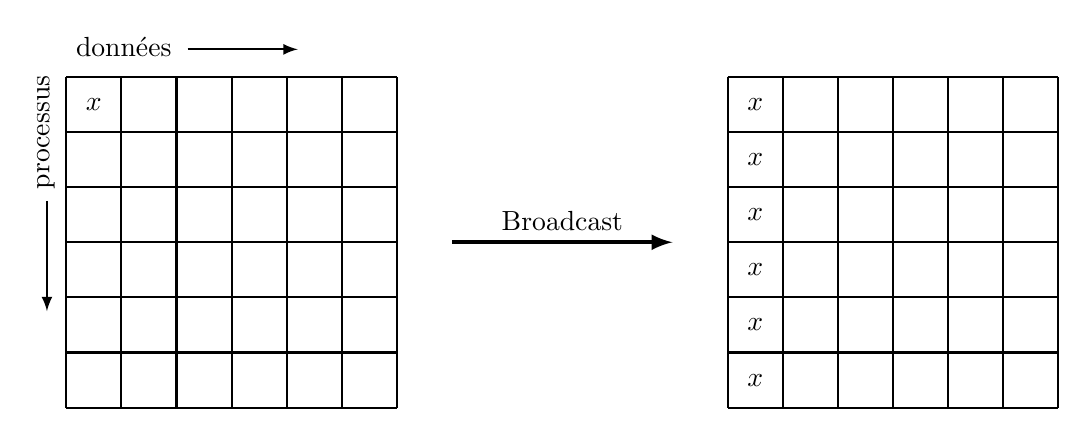
\begin{tikzpicture}[scale=0.7, >=latex]
%Bcast
\begin{scope}
  \begin{scope}
    % légendes
    \path (0, 6.2) node[above right] {données};
    \draw[thick,->] (2.2, 6.5) -- +(2, 0);

    \path (-0.7, 6.2) node[below left,rotate=90] {processus};
    \draw[thick,->] (-0.35, 3.75) -- +(0, -2);

    \foreach \i in {0,1,...,6} {
      \draw[thick] (\i, 0) -- +(0, 6);
      \draw[thick] (0, \i) -- +(6, 0);
    }
    \node at (0.5, 5.5) {$x$};
  \end{scope}

\draw[ultra thick,->] (7, 3) -- node[above] {Broadcast} (11, 3);

\begin{scope}[xshift=12cm]
  \foreach \i in {0,1,...,6} {
    \draw[thick] (\i, 0) -- +(0, 6);
    \draw[thick] (0, \i) -- +(6, 0);
  }
  \foreach \i in {0,1,...,5}
    \node at (0.5, 5.5-\i) {$x$};
\end{scope}
\end{scope}
\end{tikzpicture}
\end{center}

\paragraph{Dispersion et rassemblement}

\begin{minted}{C}
int MPI_Gather(const void* sendbuf, int sendcount, MPI_Datatype sendtype,
                     void* recvbuf, int recvcount, MPI_Datatype recvtype,
               int root, MPI_Comm comm);
int MPI_Scatter(const void* sendbuf, int sendcount, MPI_Datatype sendtype,
                      void* recvbuf, int recvcount, MPI_Datatype recvtype,
                int root, MPI_Comm comm);
\end{minted}

L'opération \og \anglais{Gather}\fg (littéralement \og rassembler\fg)
rassemble sur le processus \verb|root| des données éparpillées sur
tous les autres processus. Chaque processus transfère vers \verb|root|
les \verb|sendcount| éléments de son tableau \verb|sendbuf|.

Sur le processus \verb|root|, toutes les données de tous les processus
atterrissent dans le tableau \verb|recvbuf|, qui doit donc être de taille
$\verb|sendcount| \cdot P$, où $P$ désigne le nombre de processus du
communicateur \verb|comm|. Si $\verb|sendbuf|_i$ désigne le tableau du $i$-ème
processus, alor le résultat de l'opération est :
\[
\verb|recvbuf|[i\cdot \verb|sendcount| : (i+1)\cdot \verb|sendcount|] \gets \verb|sendbuf|_i, \qquad 0 \leq i < P
\]

\begin{danger}
  Les arguments \verb|sendcount| et \verb|sendtype| doivent partout être égaux
  aux valeurs de \verb|recvcount| et \verb|recvtype| sur \verb|root|. Cela
  signifie que sur \verb|root|, \verb|recvcount| indique le nombre d'élément
  reçus depuis chaque autre processus, et pas le nombre total d'éléments reçus.
\end{danger}

\begin{ddanger}
  Il existe deux fonctions \verb|MPI_Gatherv| et \verb|MPI_Scatterv| qui
  permettent de transférer un nombre d'éléments qui n'est pas le même pour
  chaque processus du communicateur.
\end{ddanger}

Les arguments décrivant le tableau de destination sont ignorés par la fonction,
excepté sur le processus \verb|root| (donc ailleurs on peut mettre n'importe
quoi).

Un petit détail : même sur \verb|root|, il faut donner un \verb|sendbuf|
valable, dont le contenu sera copié (en RAM) dans \verb|recvbuf|. Comme ceci
n'est pas forcément souhaitable, on peut passer à la place de \verb|sendbuf| la
valeur spéciale \verb|MPI_IN_PLACE|. Dans ce cas, aucun transfert n'a lieu de
\verb|root| vers lui-même. Ceci est adapté au cas où les bonnes données sont
déjà au bon endroit dans \verb|recvbuf|.

\begin{center}
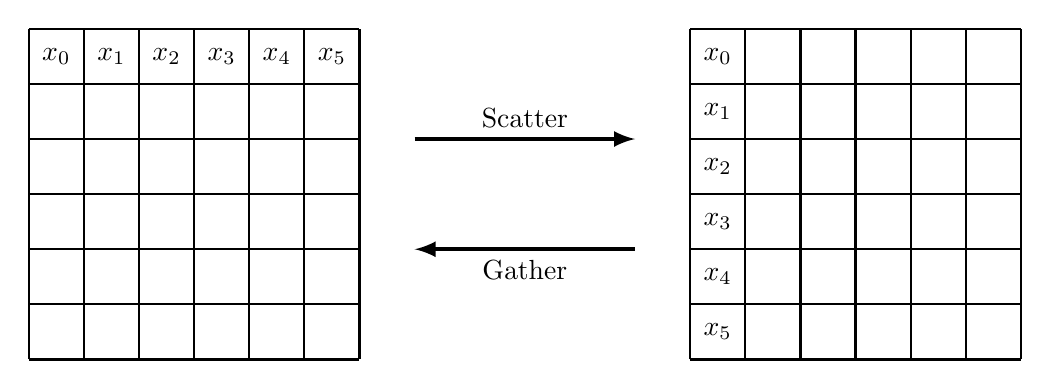
\begin{tikzpicture}[scale=0.7, >=latex]

%%%%%%%%%%%% Scatter / Gather
  \begin{scope}
    \foreach \i in {0,1,...,6} {
      \draw[thick] (\i, 0) -- +(0, 6);
      \draw[thick] (0, \i) -- +(6, 0);
    }
    \foreach \i in {0,1,...,5}
    \node at (\i+0.5,  5.5) {$x_\i$};
  \end{scope}

\draw[ultra thick,->] (7, 4) -- node[above] {Scatter} (11, 4);
\draw[ultra thick,<-] (7, 2) -- node[below] {Gather} (11, 2);

\begin{scope}[xshift=12cm]
  \foreach \i in {0,1,...,6} {
    \draw[thick] (\i, 0) -- +(0, 6);
    \draw[thick] (0, \i) -- +(6, 0);
  }
  \foreach \i in {0,1,...,5}
    \node at (0.5, 5.5-\i) {$x_\i$};
\end{scope}
\end{tikzpicture}
\end{center}

L'opération \og \anglais{Scatter}\fg (\og dispersion\fg) est l'exact
opposé. Les éléments d'un gros tableau sur \verb|root| sont répartis
sur les $P$ processus du communicateur. Les arguments ont les mêmes
significations. Cette fois cependant, la description du tableau
d'envoi est ignorée sur tous les autres processus que \verb|root|.

Sur \verb|root|, il est possible de passer \verb|MPI_IN_PLACE| à la
place de \verb|recvbuf|. Dans ce cas-là, aucune donnée n'est
transférée de \verb|root| vers lui-même.

\paragraph{All-Gather}

\begin{minted}{C}
int MPI_Allgather(const void* sendbuf, int sendcount, MPI_Datatype sendtype,
                        void* recvbuf, int recvcount, MPI_Datatype recvtype, MPI_Comm comm);
\end{minted}

La fonction \og All-gather\fg est un équivalent de \verb|MPI_Gather|, à ceci
près que le résultat n'arrive pas uniquement sur un processus racine, mais sur
tous les processus du communicateur. Par conséquent, les \verb|sendcount| et
\verb|recvcount| doivent être égaux partout, et partout égaux entre eux (on se
demande pourquoi il faut donner deux fois...).

Si \emph{tous} les processus utilisent la valeur spéciale
\verb|MPI_IN_PLACE|, alors les tableaux d'envoi sont ignorés. Les
données envoyées par le $i$-ème processus à tous les autres sont alors
lues dans le tableau de destination, à l'endroit où auraient atterri
celles qu'ils se serait envoyé lui-même.

\begin{center}
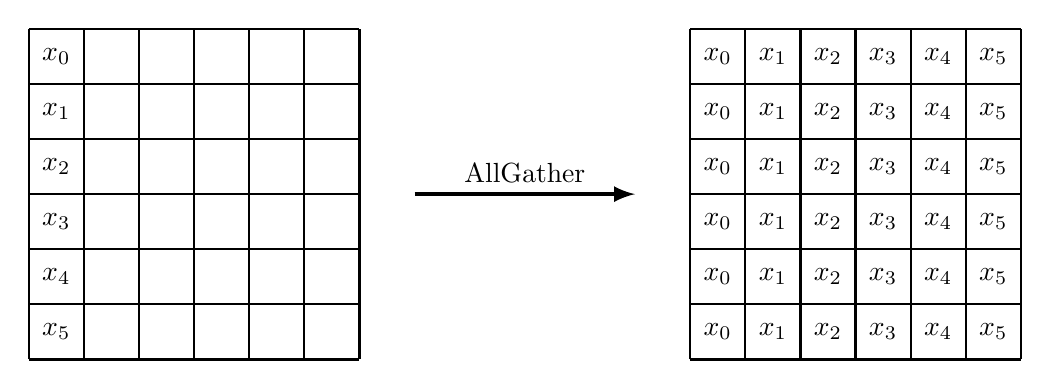
\begin{tikzpicture}[scale=0.7, >=latex]
  \begin{scope}
    \foreach \i in {0,1,...,6} {
      \draw[thick] (\i, 0) -- +(0, 6);
      \draw[thick] (0, \i) -- +(6, 0);
    }
    \foreach \i in {0,1,...,5}
    \node at (0.5,  5.5-\i) {$x_\i$};
  \end{scope}

\draw[ultra thick,->] (7, 3) -- node[above] {AllGather} (11, 3);

\begin{scope}[xshift=12cm]
  \foreach \i in {0,1,...,6} {
    \draw[thick] (\i, 0) -- +(0, 6);
    \draw[thick] (0, \i) -- +(6, 0);
  }
  \foreach \i in {0,1,...,5}
  \foreach \j in {0,1,...,5}
  \node at (\i+0.5, \j+0.5) {$x_\i$};
\end{scope}
\end{tikzpicture}
\end{center}

\begin{ddanger}
  Il existe une fonction \verb|MPI_Allgatherv| qui permett de transférer un
  nombre d'éléments qui n'est pas le même pour chaque processus du
  communicateur.
\end{ddanger}

Si on n'avait pas \verb|MPI_Bcast|, on pourrait obtenir le même effet en
utilisant une combinaison des autres fonctions : \verb|MPI_Bcast| est équivalent
à \verb|MPI_Scatter| suivi de \verb|MPI_Allgather|.

De même \verb|MPI_Allgather| est équivalent à \verb|MPI_Gather| suivi de \verb|MPI_Bcast|.

\paragraph{All-to-All}

\begin{minted}{C}
int MPI_Alltoall(const void* sendbuf, int sendcount, MPI_Datatype sendtype,
                       void* recvbuf, int recvcount, MPI_Datatype recvtype,
                 MPI_Comm comm);
\end{minted}

Cette fonction est une variante généralisée de la précédente. Dans
\verb|MPI_Allgather|, le processus de rang $i$ envoie ses données à
tous les autres processus : il leur envoie la même chose à
chacun. Dans \verb|MPI_Alltoall|, le processus $i$ envoie la $j$-ème
\og portion\fg de son tableau au processus de rang $j$. C'est un peu
comme si tous les processus dispersaient leurs tableaux en même temps.

Les \verb|sendcount| et  \verb|recvcount| doivent être égaux partout,
et partout égaux entre eux (on se demande donc pourquoi il faut les
donner deux fois...).

Les deux \anglais{buffers} doivent être disjoints et ne pas se chevaucher. Mais
si \emph{tous} les processus passent la valeur spéciale \verb|MPI_IN_PLACE| à la
place de \verb|sendbuf|, alors les données à envoyer sont lues dans
\verb|recvbuf|, et elles sont écrasées par les données reçues.

\begin{ddanger} Il existe aussi \verb|MPI_Alltoallv| et \verb|MPI_Alltoallw| qui
  offrent plus de flexibilité.
\end{ddanger}

\begin{center}
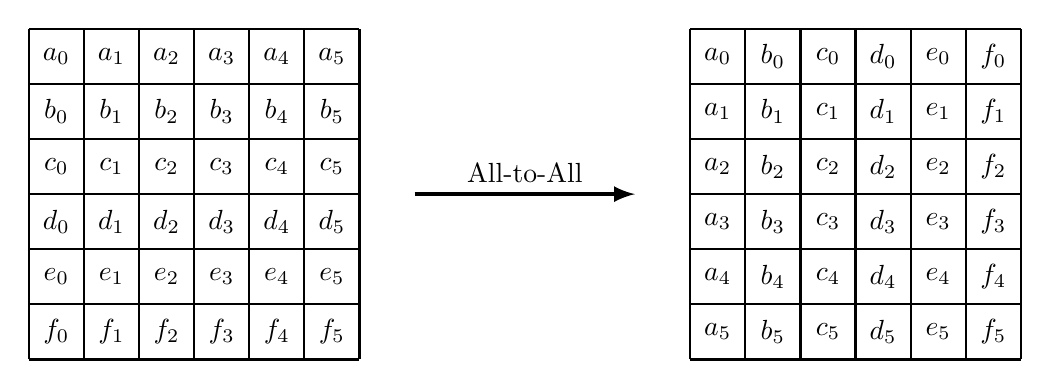
\begin{tikzpicture}[scale=0.7, >=latex]

%%%%%%%%%%%% All-to-All
  \begin{scope}
    \foreach \i in {0,1,...,6} {
      \draw[thick] (\i, 0) -- +(0, 6);
      \draw[thick] (0, \i) -- +(6, 0);
    }
    \foreach \i in {0,1,...,5}
    \foreach \letter / \j in {a/5, b/4, c/3, d/2, e/1, f/0}
    \node at (\i+0.5, \j+0.5) {$\letter_\i$};
  \end{scope}

\draw[ultra thick,->] (7, 3) -- node[above] {All-to-All} (11, 3);

\begin{scope}[xshift=12cm]
  \foreach \i in {0,1,...,6} {
    \draw[thick] (\i, 0) -- +(0, 6);
    \draw[thick] (0, \i) -- +(6, 0);
  }
  \foreach \i in {0,1,...,5}
    \foreach \letter / \j in {a/0, b/1, c/2, d/3, e/4, f/5}
    \node at (\j+0.5, 5.5-\i) {$\letter_\i$};
\end{scope}
\end{tikzpicture}
\end{center}

\subsection{Opérations de \og réduction\fg}

Les opérations de réduction consistent à appliquer une opération
(somme, produit, min, max, etc.) sur des données qui sont réparties
sur les différents processus d'un communicateur. Il faut à chaque fois
préciser l'opération. Il est possible de définir ses propres
opérations, mais les bibliothèques MPI en fournissent déjà un certain
nombre : \verb|MPI_MAX|, \verb|MPI_MIN|, \verb|MPI_SUM|,
\verb|MPI_PROD|, dont les significations sont transparentes.

\paragraph{Reduce}
\begin{minted}{C}
int MPI_Reduce(const void* sendbuf, void* recvbuf, int count, MPI_Datatype datatype,
               MPI_Op op, int root, MPI_Comm comm)
\end{minted}

Cette fonction combine, élément par élément, les différents tableaux
\verb|sendbuf| de tous les processus. Le résultat se trouve dans le
tableau \verb|recvbuf| sur le processus \verb|root|. Plus précisément,
il se passe :
\[
\verb|recvbuf|[j] \gets \verb|sendbuf|_0[j] \oplus \verb|sendbuf|_1[j]
\oplus \dots \oplus \verb|sendbuf|_{P-1}[j], \qquad 0 \leq j < \verb|count|
\]
Comme d'habitude, $P$ désigne la taille du communicateur, et $\oplus$
désigne l'opération sélectionnée. La valeur de \verb|recvbuf| est
ignorée ailleurs que sur \verb|root| (donc on peut mettre n'importe
quoi).

Sur \verb|root|, il est possible de passer \verb|MPI_IN_PLACE| à la
place de \verb|sendbuf|. Dans ce cas-là, la \og contribution\fg de
\verb|root| est prise dans \verb|recvbuf|.

\paragraph{All-Reduce}

Il y a deux variantes de \verb|MPI_Reduce| qui diffèrent par le
placement des résultats au sein du communicateur. Ces deux variantes
sont simulables à partir des autres opérations, mais existent
séparément pour des questions de performance. On rappelle que dans
\verb|MPI_Reduce| le résultat des calculs est rapatrié sur un
processus spécifique.

\begin{minted}{C}
int MPI_Allreduce(const void* sendbuf, void* recvbuf, int count,
                  MPI_Datatype datatype, MPI_Op op, MPI_Comm comm);
\end{minted}

Cette fonction se comporte comme \verb|MPI_Reduce|, mais au lieu que
les résultats soient concentrés sur une \og racine\fg, ils sont \og
broadcastés\fg sur l'ensemble des processus. C'est exactement comme si
on faisait :
\begin{verbatim}
MPI_Reduce(sendbuf, recvbuf, count, datatype, op, root, comm);
MPI_Bcast(recvbuf, count, datatype, root, comm);
\end{verbatim}

Il y a une variante \og en place\fg : si \emph{tous} les processus
passent \verb|MPI_IN_PLACE| à la place de \verb|sendbuf|, alors les
données sont lues dans \verb|recvbuf|.

\paragraph{Reduce-Scatter}
\begin{minted}{C}
int MPI_Reduce_scatter_block(const void* sendbuf, void* recvbuf, int recvcount,
                             MPI_Datatype datatype, MPI_Op op, MPI_Comm comm);
\end{minted}

Celle-ci se comporte comme \verb|MPI_Reduce|, mais les résultats sont
dispersés sur l'ensemble des processus. C'est exactement comme si on
faisait :
\begin{minted}{C}
MPI_Reduce(sendbuf, tempbuf, count, datatype, op, root, comm);
MPI_Scatter(tempbuf, count, datatype, recvbuf, count, datatype, root, comm);
\end{minted}

Il y a aussi une variante \textit{in-place}, qui fonctionne comme la précédente.

\section{Partitionnement des communicateurs}

Il est parfois souhaitable de pouvoir effectuer des opérations collectives sur
une partie seulement de l'ensemble des processus MPI. Lorsqu'une application MPI
démarre, un seul communicateur est disponible, \verb|MPI_COMM_WORLD| qui
contient l'ensemble de tous les processus.

Pour cela, un mécanisme permet de partitionner un communicateurs en plusieurs
sous-communicateurs.

\begin{minted}{C}
int MPI_Comm_split(MPI_Comm comm, int color, int key, MPI_Comm *newcomm);
\end{minted}

Cette fonction est une opération collective (donc \emph{tous} les processus du
communicateur \verb|comm| doivent l'appeler). Chaque processus peut spécifier
une valeur arbitraire de \verb|color| et de \verb|key|. Chaque processus
récupère un nouveau communicateur \verb|newcomm|, dont il fait partie.

Tous les processus qui ont indiqué la même \verb|color| appartiennent au même
(sous-)communicateur \verb|newcomm|. Au sein de \verb|newcomm|, les processus
ont des rangs ($0, 1, 2, \dots$) ; ils sont numérotés par valeur de \verb|key|
croissante (leur rang dans l'ancien communicateur \verb|comm| sert à départager
les cas d'égalité).

Le même communicateur de départ peut être découpé plusieurs fois de plusieurs
manière différentes. Un exemple typique est celui où les processus sont disposés
sur une grille en deux dimensions. Il est alors commun de former des
sous-communicateurs pour les lignes et les colonnes.

\chapter{Un peu d'algorithmique parallèle}

\section{Introduction}

Pour effectuer un calcul parallèle, il faut réussir à le découper en petites
tâches et à répartir ces tâches sur les différents processeurs. Sur une machine
à mémoire distribuée, il faut aussi que les \emph{données} nécessaires aux
calculs soient elles-mêmes réparties. La manière d'agencer cette répartie est
parfois le problème principal du calcul parallèle.

Le cas le plus simple est celui d'un tableau de taille $n$ réparti entre $p$
processeurs : chaque processeur possède une portion de taille $n/p$ du
tableau. Plus précisément, le processeur de rang $i$ possède
$A\left[i \frac{n}{p} : (i+1) \frac{n}{p}\right]$. On parle alors de répartition
\og par bloc\fg.

Dans ce contexte, le motif générique de la \og transformation\fg (\anglais{map})
est facile à paralléliser :
\begin{minted}{C}
for (int i = 0; i < n; i++)
   B[i] = f(A[i], i)
\end{minted}

Tous les \mintinline{C}{B[i]} peuvent être calculés indépendamment les uns des
autres en parallèle : chaque processeur calcule \og sa\fg portion du tableau $B$
à partir de \og sa\fg portion du tableau $A$. Les différents processeurs n'ont
pas besoin de communiquer. Si le temps de calcul de $f$ ne dépend pas trop de la
valeur de ses arguments, alors la charge de calcul sera équitablement répartie.

\subsection{Algorithmes de \og réduction\fg}

Le cas de la \og réduction\fg (\anglais{reduce}) est un peu plus compliqué :
\begin{minted}{C}
double sum = 0;
for (int i = 0; i < n; i++)
   sum = sum + A[i];
\end{minted}

Les itérations de la boucle ne peuvent pas être exécutées en parallèle, car
elles ne sont pas indépendantes (elles lisent et écrivent la même variable
\verb|Sun|). En fait, il y a des critères simples et formels (les \og conditions
de Bernstein\fg) qui permettent de décider si deux opérations $O_1; O_2$ (qui
doivent être exécutées séquentiellement) peuvent en fait être exécutées en
parallèle sans modifier leur résultat. Il faut :
\begin{enumerate}[$i$)]
\item Qu'aucune variable lue par $O_1$ ne soit écrite par $O_2$.
\item Qu'aucune variable écrite par $O_1$ ne soit écrite par $O_2$.
\item Qu'aucune variable lue par $O_2$ ne soit écrite par $O_1$.
\end{enumerate}

Dans l'exemple de la réduction, les conditions ne sont pas remplies à cause de
\verb|sum|. Il faut donc légèrement modifier l'algorithme. Par exemple, on
pourrait envisager la solution suivante (pour une machine à mémoire partagée) :

\algbegin Algorithme S (Somme d'un tableau). Il s'agit de calculer la somme d'un
tableau $A$ de $n$ éléments sur une machine où $p$ processeurs partagent la
mémoire. On suppose que $n$ est un multiple de $p$ pour se simplifier la vie.

\algstep S0. [Initialisation]. Allouer un tableau \texttt{Scratch} de taille $p$ dans la mémoire partagée.

\algstep S1. [Somme locale]. Pour $0 < i < p$, le processeur $\#i$ fait :
$\texttt{Scratch[i]} \gets \texttt{sum(A[i*n/p : (i+1)*n/p])}$. Ceci est fait en
parallèle par tous les processeurs, il n'y a pas de dépendance de données.

\algstep S2. [Barrière]. Attendre que tous les processeurs aient fini l'étape précédente.

\algstep S3. [Portion séquentielle]. Le processeur $\#0$ calcule la somme du
tableau \texttt{Scratch} puis l'écrit dans la variable \texttt{sum}.

\algstep S4. [Barrière]. Tous les processeurs attendent que le processeur \#0
ait fini l'étape précédente.

\algstep S5. [Finalisation]. Libérer le tableau \texttt{Scratch}.

L'étape S1 nécessite un temps $n/p$ sur chacun des $p$ processeurs. L'étape S3 a
une complexité en temps de $p$. Le temps total nécessaire à l'exécution de
l'algorithme est donc de $n/p+p$. Ceci atteint un minimum de $2\sqrt{n}$ lorsque
$p=\sqrt{n}$. Au-delà de cette limite, ajouter des processeurs \emph{augmente}
le temps d'exécution (c'est la limite classique au \anglais{strong scaling} dont
il est question §~\ref{sec:strong-scaling}).



\algbegin Algorithme R (Somme d'un tableau, méthode en arbre). Mêmes hypothèses
que pour l'algorithme S. 

\algstep R0. [Fini ?]. Si $n = 1$, renvoyer $A[0]$.

\algstep R1. [Initialisation]. Allouer un tableau \texttt{Scratch} de taille
$\lceil n / 2 \rceil$ dans la mémoire partagée.

\algstep R2. [Somme]. Pour tout $0 \leq i < n/2$, faire (en parallèle)~: $\texttt{Scratch}[i] \gets A[2i] + A[2i+1]$. Enfin, si $n$ est impair, faire $\texttt{Scratch}[n/2] \gets A[n-1]$.

\algstep R3. [Récursion]. Invoquer l'algorithme R récursivement pour calculer la
somme du tableau \texttt{Scratch} (de taille $\lceil n/2 \rceil$). Stocker le
résultat dans une variable $x$.

\algstep R4. [Finalisation]. Libérer le tableau \texttt{Scratch} et renvoyer $x$.


Si on dessine le \og flot\fg des données entre les différentes étapes de
l'algorithme R, on s'aperçoit qu'il forme un arbre binaire (qui est complet si
l'entrée est de taille $2^n$), dans lequel l'information monte des feuilles vers
la racine.

Comme il y a été fait allusion au §~\ref{sec:strong-scaling}, le nombre total
d'opérations élémentaires effectuées par un algorithme parallèle est son
\emph{travail}, et on le note $W(n, p)$ --- parfois seulement $W(n)$ s'il ne
dépend pas de $p$, ce qui est souhaitable ---, où $n$ désigne la taille de
l'entrée et $p$ le nombre de processeurs.

L'étape R2 nécessite $n/2$ opérations, et tout le reste est négligeable en
dehors de l'appel récursif. On a donc :
\begin{align}
  W(n) &= \frac{n}{2} + W(n/2) \\
       &= \frac{n}{2} + \frac{n}{4} + \frac{n}{8} +  \dots + 1\\
       &= n \times \left( \frac{1}{2} + \frac{1}{4} + \frac{1}{8} +  \dots + \frac{1}{n} \right)\\
       & \leq n
\end{align}

Le nombre d'appel récursif est précisément de $\lceil \log_2 n \rceil$. Tant que
$p \leq n/2$, alors on peut affirmer que l'étape R2 nécessite un temps
$\frac{n}{2p}$ avec $p$ processeurs. Le tout va donc prendre un temps
$n/p + \log_2 p$, qui est minimal lorsque $p=n/2$ et vaut alors $1 + \log_2 n$.

De plus, dans le cas d'une machine à mémoire distribuée, des communications
seront fatalement nécessaires entre les processeurs, car aucun ne possède
entièrement le tableau $A$, donc aucun ne peut calculer \verb|sum| tout seul. La
coopération est nécessaire. La solution la plus simple à programmer \og à la
main\fg est probablement celle de l'algorithme S. Heureusement, il y a
\verb|MPI_Reduce|... 

\section{Un cas non-trivial : les somme-préfixes}

Enfin, il y a des opérations encore plus complexes et plus difficiles à
paralléliser. Par exemple, le tri :
\begin{minted}{C}
B = sort(A);
\end{minted}

Ou le calcul des \og sommes-préfixes\fg :
\begin{minted}{C}
for (int i = 1; i < n; i++)
   A[i] = A[i] + A[i - 1];
\end{minted}

Il semble que chaque itération dépende du résultat de l'itération précédente, ce
qui forcerait \textit{a priori} à effectuer le calcul séquentiellement. Dans ce
cas précis, ce n'est pas vrai, mais il faut \emph{modifier l'algorithme} assez
sensiblement pour pouvoir le paralléliser.

\medskip
\begin{algorithmic}[1]
  \Function{Prefix-Sum}{A}

  \State $n$ désigne la taille de $A$
  \State Si $n = 1$, alors \Return

  \State $k \gets \left\lceil n/2\right\rceil$
  \State Allouer un tableau $B$ de taille $k$

  \ParallelFor[$0 \leq i < n / 2$]
    \State $B[i] \gets A[2i] + A[2i+1]$
  \EndParallelFor
  \State Si $n$ est impair, alors $B[k - 1] \gets A[n - 1]$

  \State $\Call{Prefix-Sum}{B}$

  \ParallelFor[$1 \leq i < n$]
  \State Si $i$ est impair, alors $A[i] \gets B[(i-1)/2]$.
  \State Si $i$ est pair, alors $A[i] \gets B[i/2-1] + A[i]$.

  \EndParallelFor

  \EndFunction
\end{algorithmic}

Un raisonnement similaire à l'analyse de l'algorithme R montre que
$W(n) = \frac{3}{2}n + W(n/2) = 3n \left( \frac{1}{2} + \frac{1}{4} + \dots +
  1\right) \approx 3n$. La quantité totale d'opération est \emph{trois fois plus
  importante} que dans le cas de l'algorithme séquentiel naïf. Par conséquent,
l'accélération parallèle sera majorée par $1/3$. Autrement dit, même avec 3
processeurs cet algorithme ne peut pas battre l'algorithme séquentiel naïf. Mais
on peut se convaincre que tant que $p \leq n$, on va avoir un temps d'exécution
parallèle de l'ordre de $3n/p + \log_2 n$.

Si on compare le flot des données dans le calcul avec le calcul de la somme, on
se rend compte qu'on a cette fois affaire à un arbre binaire complet où les
données montent jusqu'à la racine, puis, dans une deuxième phase, redescendent
jusqu'aux feuilles.


\section{Opérations collectives dans MPI}

\subsection{Modèles du coût de transfert d'un message}

Combien de temps nécessite la transmission d'un message ? En général
c'est très compliqué à prédire, car cela dépend de la topologie du
réseau, de la charge des machines, du système d'exploitation, de la
qualité des cables, du nombre de \anglais{switches} à traverser et de
leur qualité, de la congestion du réseau, etc.

On peut trouver dans la littérature des modèles précis pour des
machines particulières.

Cependant, on peut quand même essayer de dire des choses générales. Il y a de
nombreux modèles mathématiques, plus ou moins sophistiqués et qui décrivent plus
ou moins fidèlement ce qui peut se passer.

Le plus simple consiste à considérer que le temps de transfert d'un message de
$S$ octets est $T(S) = \alpha + \beta \cdot S$. Le terme $\alpha$ représente la
latence du réseau, des OS, de la bibliothèque MPI, etc. Le terme $\beta$ lui
représente le temps mis pour transférer un octet (c'est l'inverse de la bande
passante). Ceci n'est vrai qu'approximativement, et surtout pour les grands
messages. %J'ai pu mesurer dans les salles de TP de Polytech'Lille
%qu'envoyer des messages de 8 octets est \emph{plus long} (!) que des
%messages de 80 octets.

\subsection{Algorithmes pour \textsc{Scatter}, \textsc{Gather}}

Tout d'abord, notons que \anglais{Scatter} et \anglais{Gather} sont des
opérations réciproques. Par conséquent, un algorithme pour l'un
devient un algorithme pour l'autre  si on y inverse l'ordre et le sens
des communications.

Tout d'abord, on peut dire des choses générales. Si $p$ désigne la taille du
communicateur et $n$ la taille du tableau à disperser (resp. rassembler), alors
on sait qu'un volume de données $(p-1) n / p$ doit sortir (resp. entrer) du
processus racine à un moment ou à un autre ($p-1$ portions de taille $n/p$). Par
conséquent, l'opération va prendre un temps supérieur à
$(p-1) \cdot n / p \beta$. D'autre part, on sait aussi que ceci nécessite
l'envoi d'un certain nombre de messages successivement, et donc prendre un temps
supérieur à $\alpha \log_2 p$. En effet, si on imagine le \textsc{Scatter} comme
la diffusion d'une épidémie, alors au début il y a un seul malade (la \og
racine\fg). S'il a le temps d'envoyer un seul message, il peut en contaminer UN
autre. Mais si ces deux malades ont de nouveau le temps d'envoyer un nouveau
message, ils peuvent en contaminer DEUX autres, etc. De la sorte, le nombre de
malades double à chaque étape, mais ça ne peut pas aller plus vite que ça. Il
faut donc au moins $\log_2 p$ étapes qui prennent chacune un temps minoré par
$\alpha$.

Par conséquent, on trouve :
\[
T_{\mathrm{scatter}} \geq \alpha \log_2 p + (p-1)\frac{n}{p} \beta
\]

\paragraph{Méthode \og \emph{flat-tree}\fg }

Pour faire \textsc{Scatter} avec un message de taille $n$ sur $p$ processus, la
solution la plus simple consiste en ce que la racine envoie sa \og tranche\fg à
chacun des autres processus de manière séquentielle.

Combien de temps ceci va-t-il prendre ? Le plus gros problème se situe-t-il dans
le terme de latence ou dans celui de volume (ou les deux ?)

Les messages sont de taille $n/p$. D'après le modèle, le temps nécessaire à
l'envoi d'un de ces messages est $\alpha + n/p \cdot \beta$. Le processus racine
garde sa part, et il envoie $p-1$ messages aux autres avec leurs parts. Le tout
prend donc un temps :
\[
 (p-1) \left(\alpha + \frac{n}{p} \beta\right) = (p-1) \alpha + (p-1)\frac{n}{p} \beta
\]
Le terme de volume est le même que dans la borne inférieure : il est
donc optimal. Par contre le temps de latence est trop grand. Il est
linéaire alors que la borne inférieure est logarithmique.

Pour gagner du temps, on peut exploiter du parallélisme. Cette
stratégie d'organisation des communications est assez générale et
s'applique à de nombreuses situations.

\paragraph{Méthode de l'arbre binaire} Supposons que les processus soient
numérotés à partir de 1 (en pratique il suffit d'ajouter un à leur
rang). L'idée consiste à agencer les processus sur un arbre binaire
complet. La racine est le processus 1. Le fils gauche du processus $i$
porte le numéro $2i$ et son fils droit porte le numéro $2i+1$.

\begin{center}
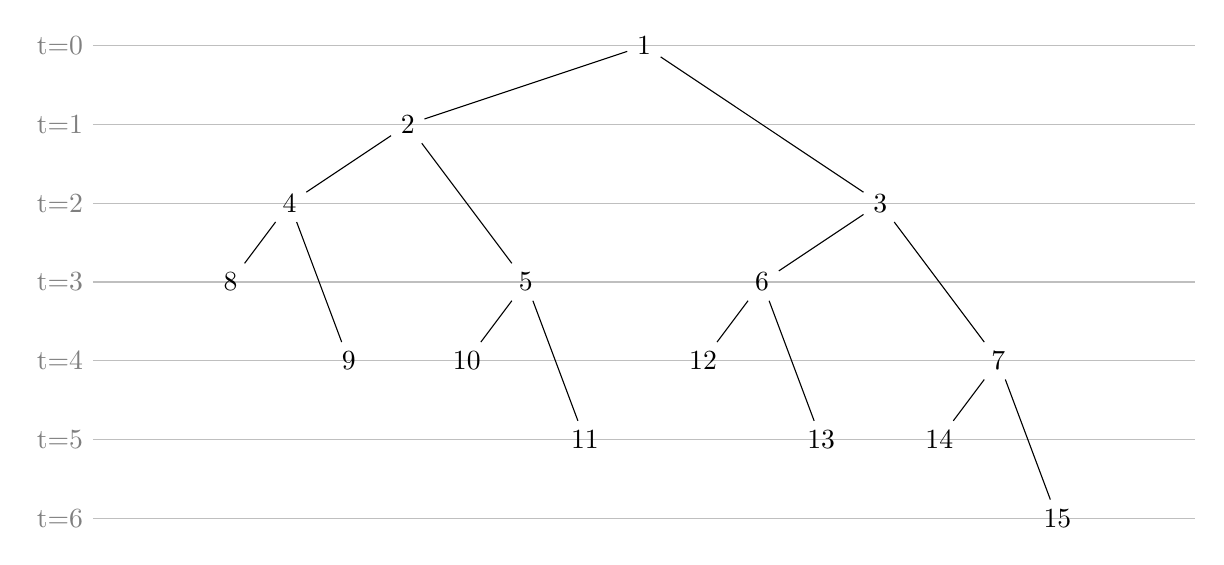
\begin{tikzpicture}[level distance=10mm]
  \foreach \i in {0,1,2,3,4,5,6} {
    \draw[semitransparent,gray] (-7, -\i) node[text=black,left] {t=\i} -- +(14, 0);
  }

  \node {1}
    child { node {2}
      child { node {4}
        child {node {8}}
        child {node at (0, -1) {9}}
      }
      child[missing]
      child {node at (0,-1) {5}
        child {node {10}}
        child {node at (0, -1) {11}}
      }
    }
    child[missing]
    child[missing]
    child[missing]
     child { node at (0, -1) {3}
      child {node {6}
        child {node {12} }
        child {node at (0, -1) {13} }
      }
      child[missing]
      child {node at (0, -1) {7}
        child {node {14}}
        child {node at (0, -1) {15} }
      }
    }
;
\end{tikzpicture}
\end{center}

L'idée c'est que 1 transmet à 2 un message qui contient non seulement la \og
portion\fg de 2, mais aussi de tous ses descendants. Il s'agit donc d'un message
dont la taille est environ la moitié de $n$. Ensuite, 1 envoie à 3 un message
qui contient sa \og portion\fg ainsi que celle de ses descendants. Dès
réception, 2 et 3 peuvent faire la même chose, en envoyant des messages de
taille $\approx n/4$ à leurs descendants.

A priori, le premier et le dernier processus à recevoir leur portion
sans en ré-emettre sont ceux qui se trouvent le plus à gauche et le
plus à droite, respectivement. Il s'agit de ceux qui portent les
numéros $2^h$ et $2^{h+1}-1$, où $h$ représente la hauteur de l'arbre,
c'est-à-dire le nombre maximal d'arêtes à traverser pour atteindre une
feuille depuis la racine. On rappelle que $h = \left\lfloor \log_2 p
\right\rfloor$.

%Combien de messages sont envoyés avant que le noeud $2^h$ ait reçu sa part ?
%Quelles sont leurs tailles ?

Il faut que tous les noeuds de la forme $2^i$ aient reçu un message de leur père
(de rang $2^{i-1}$), avant qu'ils puisse en envoyer un à leur fils gauche (de
rang $2^{i+1}$). Le nombre de messages qui doivent transiter avant que le noeud
$2^h$ ait reçu sa part est donc $h$.

Les noeuds de profondeur $i\geq 1$ (c.a.d. qui sont reliés à la racine
par un chemin qui traverse $i$ arêtes) reçoivent des messages qui
contiennent :
\[
N_i = \frac{p+1}{2^i}-1
\]
\og portions\fg du tableau de départ (on rappelle qu'une portion est de taille
$n/p$). Ceci pourrait se justifier par recurrence sur $i$ (c'est un bon exercice
qui est laissé au lecteur !). Cependant, on va se contenter de dire que les
processus de profondeur $i$ reçoivent moins de $(p-1)/2^i$ portions. En effet,
la racine cherche à répartir $p-1$ portions sur les autres processus, et chaque
processus transmet à ses enfants moins de la moitié de ce qu'il reçoit, vu qu'il
garde sa propre portion.

Le volume total de données qui circule sur le réseau avant que $2^h$
ait reçu sa part est donc :
\begin{align*}
V &= \frac{n}{p}  \sum_{i=1}^h N_i \\
   &\leq \frac{n}{p}  \sum_{i=1}^h \frac{p-1}{2^i}\\
   &\leq \frac{n}{p}  \sum_{i=1}^h \frac{1}{2^i}\\
   &\leq (p-1) \frac{n}{p}
\end{align*}

%Même question avec  ?

Pour le noeud $2^{h+1}-1$, la différence est que tous les noeuds qui se trouvent
sur le chemin qui le relie à la racine vont d'abord envoyer un message à leur
fils gauche, avant d'en envoyer un à leur fils droit. Le nombre de messages
envoyés avant que $2^{h+1}-1$ reçoive sa part est donc le double ($2h$), et le
volume de données qui doit circuler sur le réseau est aussi le double.

Voyons maintenant le temps que cette méthode requiert pour réaliser
\textsc{Scatter}. Le volume total qui doit transiter sur le réseau avant que le
dernier processus ait reçu sa part est donc de l'ordre de $2n$, tandis que le
nombre de messages qui doit circuler est de l'ordre de $2 \log p$. On va donc
avoir un temps d'exécution qui ressemble à :
\[
T \leq 2 \left\lfloor \log_2 p \right\rfloor \cdot \alpha + 2n \cdot \frac{p-1}{p}\cdot \beta.
\]
Le terme de latence est logarithmique en $p$, ce qui est un gros progrès par
rapport à la méthode précédente. Par contre, le terme de volume est \emph{deux
  fois plus gros} qu'avant. Si la taille des messages est très grande, cette
méthode risque de mettre deux fois plus longtemps que la précédente. En fait, on
obtient exactement deux fois la borne inférieure.

Un des avantages de cette méthode c'est qu'elle est très facile à programmer
même si le nombre de processus n'est pas de la forme $2^k - 1$ : il suffit
d'ignorer tous les envois à destinations de processus inexistants, qui sont tous
au dernier niveau de l'arbre, sur la droite.

\paragraph{Méthode de l'arbre binomial} On peut améliorer un peu la
méthode précédente, en remarquant que le processus racine, après avoir
glorieusement envoyé deux messages, se tourne les pouces le reste du
temps.

On peut donc lui confier davantage de travail. On suppose qu'il y a
$2^h$ noeuds numérotés de $0$ à $2^h - 1$. Au départ la racine doit
disperser un tableau qu'elle possède sur les processus de l'intervalle
$[0; 2^h[$. La procédure est la suivante :
\begin{itemize}
\item Pour disperser un tableau sur l'intervalle $[a; b[$, on repère
  le processus du milieu $c = (a+b)/2$.
\item On envoie un message contenant les portions de l'intervalle
  $[c;b]$ à $c$.
\item On s'occupe ensuite de disperser l'intervalle $[a; c[$, tandis
  que $c$ s'occupe de disperser l'intervalle $[c;b[$.
\end{itemize}

\begin{center}
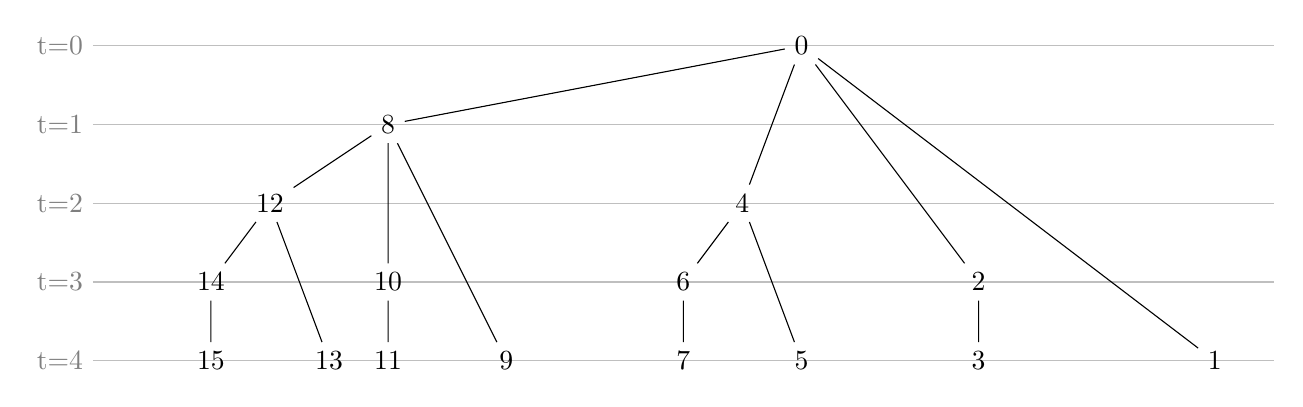
\begin{tikzpicture}[level distance=10mm]
  \foreach \i in {0,1,2,3,4} {
    \draw[semitransparent,gray] (-9, -\i) node[text=black,left] {t=\i} -- +(15, 0);
  }

  \node {0}
    child { node {8}
      child { node {12}
        child {node {14}
          child {node {15}}
        }
        child {node at (0, -1) {13}}
      }
%      child[missing]
      child {node at (0,-1) {10}
        child {node {11}}
      }
      child {node at (0,-2) {9} }
    }
    child[missing]
    child[missing]
    child { node at (0, -1) {4}
      child {node {6}
        child {node {7} }
      }
      child {node at (0, -1) {5} }
    }
    child[missing]
    child { node at (0, -2) {2}
      child {node {3}}
    }
    child[missing]
    child { node at (0, -3) {1} }
;
\end{tikzpicture}
\end{center}


Cet arbre, appelé \og arbre binomial\fg possède $2^h$ noeuds et il est
de hauteur $h$ (il réapparaît dans une structure de donnée amusante,
les \og tas binomiaux\fg).

Tous les noeuds qui sont à distance $d$ de la racine reçoivent leurs portions en
même temps. Pour voir que c'est vrai, le plus simple est d'étudier la structure
des arbres binomiaux. Ceci nous dépasse un peu, mais on va admettre qu'un arbre
binomial de hauteur $h$, qu'on notera $B_h$ est formé d'une racine, sur laquelle
sont branchés $h$ arbres binomiaux de hauteurs $0,1, 2, \dots, h-1$. Un arbre
binomial de hauteur zéro est formé d'un seul noeud. Dans le dessin ci-dessus,
\og 0\fg est la racine d'un $B_4$, tandis que \og 8\fg est celle d'un $B_3$ ;
\og 12\fg et \og 4\fg sont celles d'un $B_2$, etc.

Ceci étant dit, on voit que les noeuds qui sont les racines de $B_i$ reçoivent
tous leurs messages en même temps (ceci pourrait se justifier plus formellement
par récurrence : faites-le !). Un $B_i$ comporte $2^i$ noeuds, donc les messages
reçus par les racines de $B_i$ contiennent $2^i$ portions de taille
$p/n$. Prenons le $B_i$ le plus à gauche, et remontons le chemin qui le relie à
la racine : il reçoit son message \emph{après} que le $B_{i+1}$ qui est son père
ait lui-même reçu le message du $B_{i+2}$ qui est son propre père, etc.

Par conséquent, les $B_i$ reçoivent leur message après que $h-i$ messages aient
été envoyés, et ces messages sont de tailles respectives
$2^i, 2^{i+1}, \dots, 2^{h-1}$. Envoyer ces messages prend un temps :
\[
T = \alpha (h-i) + \beta \frac{n}{p}  \sum_{k=i}^{h-1} 2^i
\]

On en déduit le temps d'exécution de la méthode pour faire un \textsc{Scatter}
complet. Il suffit pour cela de regarder quand est-ce que les racines des $B_0$,
qui n'ont donc pas d'enfants, ont reçu leur message. D'après ce qu'on a dit
précédemment, c'est au bout d'un temps :
\begin{align*}
T &= \alpha  h + \sum_{k=0}^{h-1} 2^i\\
  &= \alpha  h + \left(2^h -1 \right) \frac{n}{p}  \beta \\
  &= \alpha  h + \left(p -1 \right)  \frac{n}{p} \beta.
\end{align*}
Et ceci est en fait \emph{exactement} la borne inférieure qu'on avait
trouvée ci-dessus.

% Le processus se termine donc après un temps :
% \[
% T = \alpha \cdot (1 + \log_2 p) + \frac{p-1}{p}\cdot n \cdot \beta
% \]

% Si $n$ est petit et que la latence domine les temps de communication,
% c'est presque deux fois plus rapide que la méthode de l'arbre binaire.

\subsection{Renversement des communications}

De la même manière que \anglais{scatter} et \anglais{gather} peuvent
être réalisés par les mêmes algorithmes \og mis à l'envers\fg, c'est
également le cas de \anglais{broadcast} et \anglais{reduce}. En effet,
dans le premier, des tableaux de taille $n$ partent de la racine et
sont envoyés à tous les processus, tandis que dans le deuxième des
tableaux de taille $n$ partent de tous les processus pour être
concentrés à la racine. Un algorithme de \anglais{broadcast} est donc
facile à transformer en algorithme de \anglais{reduce} et vice-versa.

Il en va de même pour \anglais{all-gather} et
\anglais{reduce-scatter}. Dans le premier, chaque processus récupère
une tranche de taille $n/p$ depuis chacun des autres processus. Dans
le deuxième, on récupère la \emph{somme} des tranches de taille $n/p$
de chaque autre processus. Dans les deux cas semblent donc voisins et
pourraient être implémentés de manière comparable.


\subsection{Algorithmes pour \texttt{MPI\_Allgather}}

On va voir deux méthodes différentes pour réaliser l'opération \og
All-Gather\fg, et on va tâcher de comparer, en théorie, leur performance.

\paragraph{Algorithme de l'anneau} L'idée est relativement
simple. S'il y a $p$ processus dans le communicateur, l'algorithme
s'exécute en $p$ phases. Dans la première phase, le processus $i$
envoie \og ses\fg données au processus $i+1$ (tout le monde fait ça en
même temps). Du coup, le processus $i$ reçoit les données du processus
$i-1$. Bien sûr, tout ceci se fait avec les rangs \emph{modulo $p$}.

Dans les phases suivantes, le processus $i$ transmet au processus
$i+1$ les données qu'il a reçues dans la phase précédente. De la
sorte, au bout de $p-1$ phases, tout le monde a reçu les données de tout
le monde.

Notons $n$ la quantité totale de données qui doit être rassemblée sur
chacun des processus. La \og contribution\fg de chaque processus est
donc de taille $n/p$. Dans chaque étape, chaque processus envoie et
reçoit une quantité de donnée $n/p$. Si on néglige la contention du
réseau, tous ces échanges peuvent se faire simultanément.

On s'attend donc à ce que cela prenne un temps :
\[
T_{ring} = (p-1) \alpha + (p-1)\frac{n}{p} \beta
\]

Dans cette expression, le terme de bande passante (celui avec $\beta$)
ne peut pas être amélioré : chaque processus doit recevoir $n/p$
données depuis $p-1$ autres processus. Par contre, le terme de latence
(celui avec $\alpha$) peut être amélioré.

\paragraph{Algorithme du doublage récursif} On peut en effet mettre
sur pied un algorithme très classique avec $\bigO{\log p}$ phases au
lieu de $\bigO{p}$ phases. On va supposer que le nombre de processus
est une puissance de deux, donc que $p=2^k$. Quand ce n'est pas le
cas, la technique fonctionne aussi mais les détails sont sordides.

\begin{algorithmic}[1]
  \State $r \gets \verb|MPI_Comm_Rank|()$
  \For{$0 \leq i < k$}
  \State $t \gets r ~ \texttt{XOR} ~ 2^i$
  \State Envoyer au processus de rang $t$ toutes les contributions connues
  \State Ajouter ce qu'on reçoit de $t$ à la liste des contributions connues
  \EndFor
\end{algorithmic}

Voici une illustration de l'algorithme avec $p=8$ :
\begin{center}
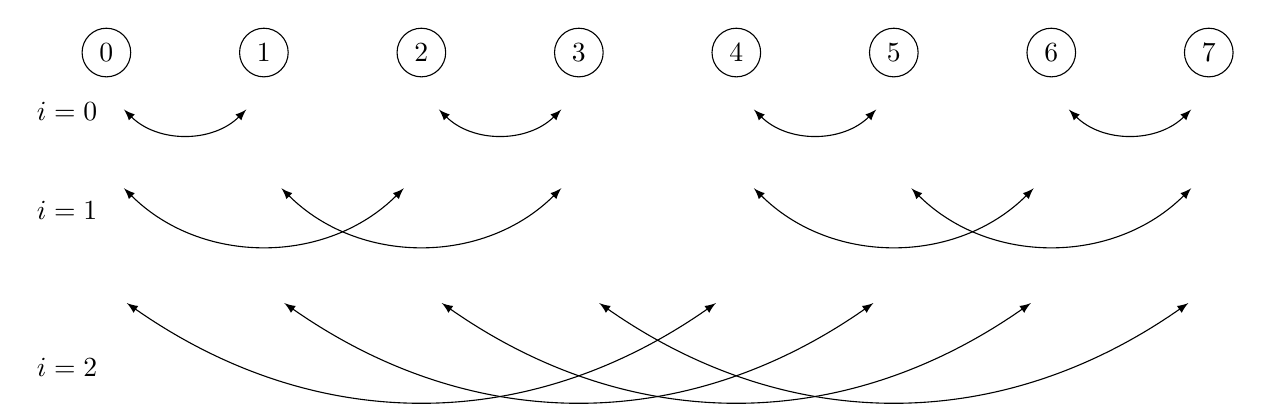
\begin{tikzpicture}[>=latex]
\foreach \i in {0,1,2,3,4,5,6,7}
  \draw (2*\i, 0) node [draw,shape=circle] (N\i) {\i};

\node at (-0.5, -0.75) {$i=0$};
\foreach \a / \b in {0/1, 2/3, 4/5, 6/7}
  \draw[<->,transform canvas={yshift=-0.5cm}] (N\a) edge [bend right=45] (N\b);

\node at (-0.5, -2) {$i=1$};
\foreach \a / \b in {0/2, 1/3, 4/6, 5/7}
  \draw[<->,transform canvas={yshift=-1.5cm}] (N\a) edge[bend right=45] (N\b);

\node at (-0.5, -4) {$i=2$};
\foreach \a / \b in {0/4, 1/5, 2/6, 3/7}
  \draw[<->,transform canvas={yshift=-3cm}] (N\a) to[bend right=35] (N\b);
\end{tikzpicture}
\end{center}

\bigskip

Chaque processus envoie et reçoit $k = \log_2 p$ messages, dont la
taille double à chaque phase. Chaque processus envoie et reçoit la
même quantité de données que dans le cas précédent. Le temps que tout
ceci prend est donc :
\[
T_{2rec} = \alpha \log_2 p + (p-1) \frac{n}{p} \beta
\]

\paragraph{Comparaison}
En théorie, il semble donc que la méthode du doublage récursif soit
incontestablement meilleure (puisque le terme de latence est toujours
plus faible). La réalité est malheureusement un peu plus
compliquée. Quand les volumes de données sont \emph{petits}, et que la
latence domine les temps de communication, l'avantage de la méthode de
doublage récursif devrait être plus prononcé --- et des études
empiriques confirment ce fait.

Par contre, quand les volumes de données sont importants, la latence
n'a plus beaucoup d'importance car c'est alors la bande passante qui
est le facteur déterminant. Les deux algorithmes ont pourtant la même
bande passante.... Mais voilà : dans l'algorithme en anneau, on ne
communique qu'avec ses \emph{voisins}, tandis que dans l'algorithme de
doublage récursif on communique avec des noeuds lointains. Selon la
configuration du réseau (liens directs avec les voisins...) on peut
obtenir moins de congestion, et une meilleure bande passante avec
l'algorithme en anneau. Sur certaines machines, l'algorithme en anneau
va deux fois plus vite dès que les messages font quelques Mo.

\subsection{Algorithmes pour  \texttt{MPI\_Bcast}}

Le \anglais{broadcast} semble être l'opération la plus simple, et pourtant... Le
même raisonnement que pour \textsc{Scatter} permet de penser qu'un temps
$\alpha \log_2 p + n\beta$ est nécessaire quoi qu'il arrive.

\paragraph{\og Flat-tree\fg} La technique la plus simple pour faire le
\anglais{broadcast} consiste à envoyer les données aux $p-1$ autres
processus successivement. Ceci prend un temps :
\[
T_{flat} = (p-1)(\alpha + n \beta)
\]

% binary tree : left child = 2*i ; right child = 2*i+1

\paragraph{\og Binomial-Tree\fg} La technique en arbre est simple (surtout si
$p=2^k$). Elle s'accomplit en $\log_2 p$ phases. Chaque processus reçoit un
message, et en expédie deux, de sorte à tracer un arbre binomial. Lors de
la première étape, \verb|root| contacte $\verb|root| + p/2$. Les deux processus
se considèrent alors comme les deux racines de deux nouveaux arbres, et
contactent chacun le processus qui est \og au milieu\fg de leurs sous-arbres
respectifs, et ainsi de suite.

Il y a $\log_2 p$ étapes, et donc le tout prend un temps :
\[
\left\lceil \log_2 p \right\rceil (\alpha + n \beta)
\]

On a donc un algorithme dont le terme de latence est optimal, mais le
terme de bande passante est $\bigO{\log p}$ fois trop grand ! Cet
algorithme est donc adapté aux \emph{petits} messages.

\paragraph{Algorithme de Van de Geijn} L'idée consiste à accomplir le
\anglais{broadcast} en effectuant d'abord un \anglais{scatter} suivi d'un
\anglais{all-gather}. En effectuant le \anglais{scatter} avec l'algorithme
optimal (en arbre binomial), on a un temps :
\[
T_{scatter} = \alpha \cdot \log_2 p + (p-1) \frac{n}{p} \beta
\]

Comme on s'intéresse en priorité au cas des grands messages, on peut
supposer qu'on utilise l'algorithme en anneau pour le
\anglais{all-gather}. Cela donne donc un temps total pour le
\anglais{broadcast} de :
\[
T = \alpha \cdot (p-1+\log_2 p) + 2 (p-1) \frac{n}{p} \beta
\]
Le terme de bande passante est meilleur que dans l'algorithme de
l'arbre binomial... Et il n'est plus que 2 fois plus grand que la
borne inférieure.

% \end{document}

% \section{TODO}

% complexité de All-to-all :

% a) tout le monde poste Isend / Irecv

% b) échange entre chaque paire en P étapes

% c) algo compliqué (cf. MPICH2)

% One-sided communications.


\section{Produit Matrice-Vecteur (dense)}

On s'intéresse à un problème qui consiste à calculer le produit d'une
matrice dense de taille $n \times n$ par un vecteur de taille
$n$. Plus précisément, on veut calculer $y = M\times x$.

Il est bien connu que l'algorithme séquentiel effectue ce calcul en
environ $n^2$ opérations.

On va supposer qu'avant le démarrage des algorithmes qu'on va
considérer, la matrice et le vecteur ont été préalablement répartis
sur les $p$ processus dont on dispose. Pour le vecteur, cela signifie
que le processus de rang $i$ possède la $i$-ème \og tranche\fg de
taille $n/p$, c'est-à-dire qu'il possède les coefficients de $x$ dans
l'intervalle :
\[
\left[ i\cdot \frac{n}{p} ; (i+1)\cdot \frac{n}{p} \right[.
\]
On veut qu'à la fin du calcul, $y$ soit réparti de la même manière. On notera
donc $x_i$ et $y_i$ les \og portions\fg qui appartiennent au $i$-ème processus.

La répartition de la matrice, elle, constitue tout l'enjeu de la discussion. On
va envisager trois stratégies.

\subsection{Stratégie n\textdegree 1 : $P_i$ possède la $i$-ème tranche des
  lignes de $M$}

Si le processus de rang $i$ (qu'on va noter $P_i$) possède la $i$-ème tranche
des lignes de $M$, alors il peut calculer la $i$-ème tranche de $y$, à condition
de connaître l'ensemble de $x$. Il n'y aura donc rien à faire pour s'assurer que
la distribution de $y$ sera correcte. Par contre, il faut \og faire venir\fg
l'ensemble de $x$ sur chaque processeur. Il s'agit d'un \og All-Gather\fg. Cela
permet de faire en sorte que tout le monde récupère toutes les \og tranches\fg
de $x$, et possède donc l'intégralité du vecteur.

\begin{center}
\begin{tikzpicture}[>=latex]
  \draw[thick] (0,0) rectangle (4,4);
  \draw[pattern=north east lines] (0, 3) rectangle +(4,0.5);
  \node[below] at (2,0) {$M$};

  \node at (4.25,2) {$\times$};

  \draw[thick,pattern=north east lines] (4.5,0) rectangle +(0.5,4);
  \node[below] at (4.75,0) {$x$};

  \draw[->] (5.25, 2) -- +(1,0);

  \draw[thick] (6.5,0) rectangle +(0.5,4);
  \draw[pattern=north east lines] (6.5, 3) rectangle +(0.5,0.5);
  \node[below] at (6.75,0) {$y$};
\end{tikzpicture}
\end{center}

On peut utiliser au maximum $n$ processeurs, car chaque processeur doit posséder
au moins une ligne de la matrice.  En terme de calculs, chaque processus doit
multiplier une matrice rectangulaire de taille $n/p \times n$ par un vecteur de
taille $n$. Ceci nécessite $n^2/p$ opérations.

Pour ce qui est des communications, c'est dans le \og all-gather\fg que tout se
passe, et on a déjà vu la complexité de cette opération. Le temps total
d'exécution de cette stratégie est donc :
\[
T= \underbrace{\frac{n^2}{p}}_{\text{calcul}} + \underbrace{\alpha \log_2 p + (p-1)\frac{n}{p} \beta}_{\text{communication}}
\]
On note qu'avec $n$ processeurs, on trouve $T= \bigO{n}$. Le temps de calcul
domine asymptotiquement les communications lorsque $n$ augmente, donc \textit{a
  minima} le \emph{weak-scaling} devrait être assez bon.


\subsection{Stratégie n\textdegree 2 : $P_i$ possède la $i$-ème tranche des
  colonnes de $M$}

Essayons de prendre le problème autrement, et d'éviter cette coûteuse
opération collective au début.

Si le processus de rang $i$ (qu'on va noter $P_i$) possède la $i$-ème
tranche des \emph{colonnes} de $M$, alors il n'a besoin que de la
$i$-ème tranche de $x$, qu'il possède déjà par hypothèse sur la
pré-distribution des données. \og Jusque-là, tout va bien\fg.

\begin{center}
\begin{tikzpicture}[>=latex]
  \draw[thick] (0,0) rectangle (4,4);
  \draw[pattern=north east lines] (3, 0) rectangle +(0.5, 4);
  \node[below] at (2,0) {$M$};

  \node at (4.25,2) {$\times$};

  \draw[thick] (4.5,0) rectangle +(0.5,4);
  \draw[pattern=north east lines] (4.5, 0.5) rectangle +(0.5,0.5);
  \node[below] at (4.75,0) {$x$};

  \draw[->] (5.25, 2) -- +(1,0);

  \draw[thick,fill=gray!50] (6.5,0) rectangle +(0.5,4);
%  \draw[pattern=north east lines] (6.5, 3) rectangle +(0.5,0.5);
  \node[below] at (6.75,0) {$y_i$};
\end{tikzpicture}
\end{center}

Le problème, c'est que le vecteur $y$ est la \emph{somme} des produits
$y_i = M_i \times x_i$ :
\[
y = \sum_{i=0}^{p-1} M_i \times x_i.
\]

Il y a donc malgré tout bien une opération de re-distribution des données, mais
en plus une opération de réduction ! Il faut calculer la somme des $y_i$ que
possèdent chaque processus, puis répartir le tout par \og tranches\fg entre tout
le monde. C'est précisément de ce que fait \og Reduce-Scatter\fg.

Comme la complexité de \og Reduce-Scatter\fg est sensiblement la même que celle
de \og all-gather\fg, et que la quantité de calcul est la même que précédemment,
on trouve une complexité comparable à celle de la première stratégie. On n'a
donc rien gagné à ce stade.

\subsection{Stratégie n\textdegree 3 : chaque processus possède un
  bloc carré de $M$}

Supposons que le nombre de processus est un carré, et donc que $\sqrt{p}$ est un
entier. On découpe la matrice $M$ en $p$ blocs carrés de taille $n / \sqrt{p}$
(distribution 2D de données 2D).

Chacun des $p$ blocs est identifié par deux coordonnées qui donnent sa
position au sein de $M$. Chacun des $p$ processus est identifié soit
par son \emph{rang} (compris entre $0$ et $p-1$), soit par ses
\emph{coordonnées cartésiennes} : le processus $(i,j)$ est celui qui
possède $M_{i,j}$.


\begin{center}
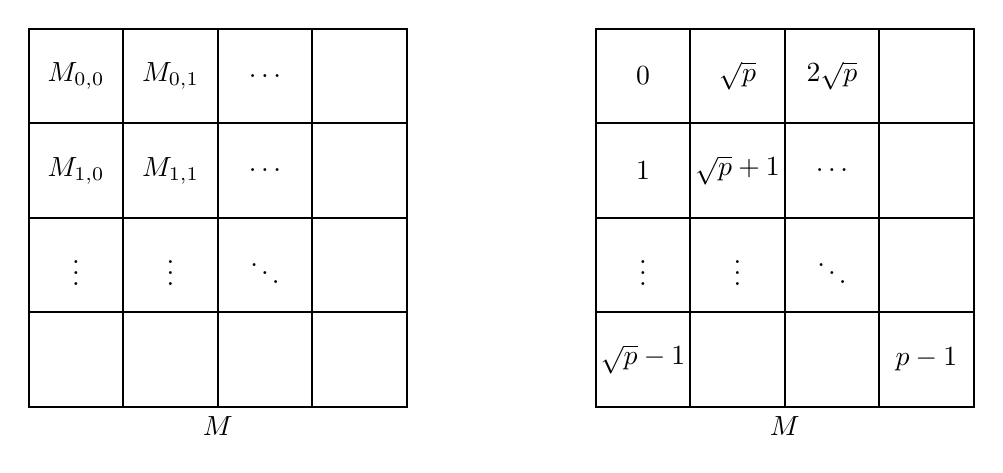
\begin{tikzpicture}[>=latex, scale=1.2]
  \draw[thick] (0,0) rectangle (4,4);
  \foreach \i in {1,2,3} {
    \draw[thick] (\i,0) -- +(0,4);
    \draw[thick] (0,\i) -- +(4,0);
  }

  \node at (0.5, 3.5) {$M_{0,0}$};
  \node at (0.5, 2.5) {$M_{1,0}$};
  \node at (0.5, 1.5) {$\vdots$};

  \node at (1.5, 3.5)  {$M_{0,1}$};
  \node at (1.5, 2.5) {$M_{1,1}$};
  \node at (1.5, 1.5)  {$\vdots$};

  \node at (2.5, 3.5)  {$\dots$};
  \node at (2.5, 2.5)  {$\dots$};
  \node at (2.5, 1.5)  {$\ddots$};

  \node[below] at (2,0) {$M$};

\begin{scope}[xshift=6cm]
  \draw[thick] (0,0) rectangle (4,4);
  \foreach \i in {1,2,3} {
    \draw[thick] (\i,0) -- +(0,4);
    \draw[thick] (0,\i) -- +(4,0);
  }

  \node at (0.5, 3.5) {$0$};
  \node at (0.5, 2.5) {$1$};
  \node at (0.5, 1.5) {$\vdots$};
  \node at (0.5, 0.5)  {$\sqrt{p}-1$};

  \node at (1.5, 3.5)  {$\sqrt{p}$};
  \node at (1.5, 2.5) {$\sqrt{p}+1$};
  \node at (1.5, 1.5)  {$\vdots$};

  \node at (2.5, 3.5)  {$2\sqrt{p}$};
  \node at (2.5, 2.5)  {$\dots$};
  \node at (2.5, 1.5)  {$\ddots$};
  \node at (3.5, 0.5)  {$p-1$};

  \node[below] at (2,0) {$M$};
\end{scope}
\end{tikzpicture}
\end{center}

La conversion entre ces deux identifiants est facile :
\begin{align*}
  r &\longrightarrow\left( r \bmod \sqrt{p}, \left\lfloor \frac{r}{\sqrt{p}}\right\rfloor \right)\\
  (i,j) &\longrightarrow i + j \cdot \sqrt{p}
\end{align*}

Le vecteur $x$ est réparti sur tous les processus comme précédemment :
le processus de rang $r$ possède la $r$-ème tranche de $x$. Cela
signifie que les processus de la première colonne de $M$ possèdent
collectivement les $\sqrt{p}$ première tranches de $x$.

Examinons maintenant le calcul que le processus $(i,j)$ doit
accomplir. Il possède $M_{i,j}$ ainsi qu'une portion de taille $n/p$
de $x$ (en noir sur le dessin de droite ci-dessous). Mais le
problème, c'est que pour calculer un produit avec $M_{i,j}$, il lui
faudrait une tranche de $x$ plus grosse, de taille $n/\sqrt{p}$
(hachurée sur le dessin) :
\begin{center}
\begin{tikzpicture}[>=latex]
  \draw[thick] (0,0) rectangle (4,4);
  \draw[thick,pattern=north east lines] (2, 2) rectangle +(1, 1);
  \node[below] at (2,0) {$M$};

  \node at (4.25,2) {$\times$};

  \draw[thick] (4.5,0) rectangle +(0.5,4);
  \draw[pattern=north east lines] (4.5, 1) rectangle +(0.5,1);
  \node[below] at (4.75,0) {$x$};

  \draw[->] (5.25, 2) -- +(1,0);

  \draw[thick] (6.5,0) rectangle +(0.5,4);
  \draw[thick,fill=gray!50] (6.5,2) rectangle +(0.5,1);
  \node[below] at (6.75,0) {$y$};

\begin{scope}[xshift=5cm]
  \draw[thick] (6.5,0) rectangle +(0.5,4);
  \draw[pattern=north east lines] (6.5,1) rectangle +(0.5,1);
  \node[below] at (6.75,0) {$x$};

  \draw[dashed] (7,1) -- +(1, 0);
  \draw[dashed] (7,2) -- +(1, 0);
  \draw[decorate,decoration={brace,mirror}] (8.2, 1) --  node[right=1mm] {taille $n/\sqrt{p}$} +(0,1);


  \draw[fill=black] (6.5,1.3) rectangle +(0.5,0.2);
  \draw[dashed] (6.5,1.3) -- +(-1, 0);
  \draw[dashed] (6.5,1.5) -- +(-1, 0);
  \draw[bend left] (5.4, 1.3) .. controls (5.3, 1.4) ..  node[left=1mm]  {taille $n/p$} +(0, 0.2);
\end{scope}

\end{tikzpicture}
\end{center}

Imaginons donc que $x$ et $y$ sont découpés à la fois en $p$ \og
petites tranches\fg de taille $n/p$, qu'on note toujours $x_i$ et
$y_i$, mais aussi en $\sqrt{p}$ \og grosses tranches\fg de taille
$n/\sqrt{p}$, qu'on notera $\widetilde{X}_i$ et $\widetilde{Y}_i$.

Chaque \og grosse tranche \og, de taille $n/\sqrt{p}$ est constituée de
$\sqrt{p}$ \og petites tranches\fg de taille $n/p$. La première grosse tranche
$\widetilde{X}_0$ est composée de $x_0, x_1, \dots, x_{\sqrt{p}-1}$. De manière
analogue, $\widetilde{X}_i$ est composé des petites tranches d'indices
$[i\cdot \sqrt{p}; (i+1)\cdot \sqrt{p}[$. Vu la numérotation des processus, ces
petites tranches se trouvent réparties sur les processus de la $i$-ème colonne.

On voit donc que le processus $(i,j)$ a besoin de $\widetilde{X}_i$ et produit une
contribution à $\widetilde{Y}_i$. On a en effet :
\[
\widetilde{Y}_i = \sum_{j=0}^{\sqrt{p}-1}  M_{i,j} \times \widetilde{X}_i,
\qquad (0 \leq i < \sqrt{p})
\]

On peut donc utiliser la procédure suivante :
\begin{enumerate}
\item Pour tout $0 \leq j < \sqrt{p}$, les processus de la colonne $j$
  collaborent pour que chacun obtienne $\widetilde{X}_i$.

\item Pour tout ($i,j)$, chaque processus calcule sa contribution
  $M_{i,j} \times \widetilde{X}_i$

\item Pour tout $0 \leq i < \sqrt{p}$, les processus de la ligne $i$
  collaborent pour calculer la somme de leurs contributions, obtenir
  ainsi $\widetilde{Y}_i$, et disperser le résultat entre eux.
\end{enumerate}

\medskip

Pour la première étape, où les processus de chaque colonne doivent mutualiser
leurs petites tranches pour former la grosse tranche dont ils ont tous besoin,
on fait un \og all-gather\fg. Pour la troisième étape, où les processus de
chaque ligne doivent sommer leur contribution, puis se la dispatcher, on fait un
\og reduce-scatter\fg. Ces deux opérations collectives concernent des tableaux
de taille $n/\sqrt{p}$, et $\sqrt{p}$ processus y participent.

Le petit détail, c'est qu'au début les $\widetilde{X}_i$ sont répartis
sur les colonnes tandis qu'à la fin les $\widetilde{Y}_i$ sont
répartis sur les lignes. Ceci peut se régler avec une dernière étape :
\begin{enumerate}
\item[4.] Pour tout($i,j)$, les processus $(i,j)$ et $(j,i)$ effectuent une
  communication point-à-point pour échanger leur petite tranche de $y$.
\end{enumerate}

La quantité de calculs est la même que précédemment : il s'agit de calculer le
produit d'une matrice carrée de taille $n/\sqrt{p}$ et d'un vecteur de la bonne
taille. Ceci nécessite $n^2/p$ opérations.

Les deux opérations collectives coûtent chacune la même chose, à savoir environ
$\alpha \log \sqrt{p} + (\sqrt{p}-1) \frac{n}{p} \beta $. Enfin, la
dernière phase de \og transposition\fg, nécessite que chaque processus envoie et
reçoive un message de taille $n/p$, donc ceci ajoute un temps
$\alpha + n/p \cdot \beta$. Au final, on trouve donc :
\[
T= \underbrace{\frac{n^2}{p}}_{\text{calcul}}
+ \underbrace{
  \left(1 + \log_2 p\right)  \alpha
  + \left(2 \sqrt{p} -1 \right) \frac{n}{p} \beta
}_{\text{communication}}
\]
Et en simplifiant un tout petit peu on obtient :
\[
T\leq  \frac{n^2}{p} + \alpha \log_2 p + 2 \frac{n}{\sqrt{p}} \beta + \bigO{1}
\]
L'intérêt principal de cette méthode est que la quantité de
communications est plus faible que dans les deux premières stratégies
(elle \emph{décroît} avec $p$).

Il est de plus possible possible d'utiliser plus de $n$ processeurs. La limite
naturelle est $n^2$ : on ne peut pas donner moins qu'un seul coefficient de la
matrice à un processeur. Mais on peut répartir la matrice en $n^2$ si on a
envie. Le petit détail, c'est qu'on ne peut pas répartir le vecteur $x$ en plus
que $n^2$. En pratique ce n'est pas un très gros problème. On peut envisager que
seuls certains processus possèdent des tranches de $x$, ou bien que plusieurs
processus possèdent la même tranche. Ce n'est pas très gênant.

Si on dispose de $p = n^2$ processeurs, le temps de calcul par processus tombe à
$\bigO{1}$, de même que le terme de volume des communications. Tout ce qui reste
est le terme de latence, qui est de l'ordre de $\bigO{\log n}$. On se heurte
alors à une borne inférieure, car chaque tranche de $y$ dépend de toutes les
tranches de $x$, or il faut $\log_2 n$ messages successifs pour que tout ce
petit monde puisse contribuer.

%\end{document}


\chapter{Programmation multi-threads avec \OMP}
\label{chap:omp}

Le principal avantage de la programmation multi-threads, c'est que les threads
partagent un même espace mémoire, ce qui leur évite d'avoir à communiquer
explicitement en se passant des messages. Mais c'est aussi une grosse source
d'erreurs, car les threads peuvent entrer en conflit les uns avec les autres
lors de l'accès aux variables partagées. Ceci nécessite la mise en place de
mécanismes de synchronisation et/ou d'exclusion mutuelle lors de l'accès aux
données partagées. \OMP le facilite, mais les performances sont parfois
problématiques.

Ce problème ne se pose pas tellement dans la programmation parallèle par passage
de messages : ce sont les communications qui synchronisent les différents
processus (notamment par l'attente de réception d'un message). Il y a des
programmeurs qui considèrent que ce modèle (\og se synchroniser par les
communications plutôt que communiquer par les synchronisations \fg) est plus
facile à mettre en oeuvre et recèle moins de sources d'erreurs subtiles. Le
langage \marque{go} développé par \marque{google} promeut cette approche.


Ce chapitre paraphrase la spécification \OMP v5.0


Modèles mémoire, séquential consistency, release consistency. Total Store
Ordering (https://www.cl.cam.ac.uk/~pes20/ppc-supplemental/test7.pdf)

https://plv.mpi-sws.org/sra/paper.pdf (section 4)

\section{Introduction à \OMP}

Standard blabla, \og \emph{lean and mean}\fg, directives du compilateur, ...

Il y a des alternatives, mais peu sont aussi populaires : \marque{Cilk} (\OMP en
est maintenant un sur-ensemble), des bibliothèques comme \marque{TBB},
\marque{Boost}, etc.

Commencer par omp parallel for

Un programme commence avec un thread initial

When any thread encounters a parallel construct, the thread creates a team of itself and zero or
more additional threads and becomes the master of the new team.
A set of implicit tasks, one per thread, is generated. The code for each task is
defined by the code inside the parallel construct.  Each task is assigned to a
different thread in the team and becomes tied; that is, it is always executed by
the thread to which it is initially assigned. The task region of the task being
executed by the encountering thread is suspended, and each member of the new
team executes its implicit task. There is an implicit barrier at the end of the
parallel construct. Only the master thread resumes execution beyond the end of
the parallel construct, resuming the task region that was suspended upon
encountering the parallel construct.

When any team encounters a worksharing construct, the work inside the construct is divided among
the members of the team, and executed cooperatively instead of being executed by every thread.
There is a default barrier at the end of each worksharing construct unless the nowait clause is
present. Redundant execution of code by every thread in the team resumes after the end of the
worksharing construct.

Nouveautés \OMP 5.0 (2018) : scan, OMPT, OMPD. Release-Acquire semantics.

Nouveautés \OMP 4.5 : fonctions de gestion de la mémoire sur les devices. Plus de thread affinity

Nouveautés \OMP 4.0 (2013) : simd. thread affinity. user-defined reductions. Dépendances entre les taches. Device directives. Atomic construct

Nouveautés \OMP 3.1 : atomic capture

Nouveautés \OMP 3.0 (2008) : tâches

Nouveautés \OMP 2.5 (2005)

Nouveautés \OMP 2.0 (2000)

Nouveautés \OMP 1.0 (1997)

Support Fortran, C, C++.

Expliquer thread vs processus (tas, pile). Fork-join. \mintinline{C}{#ifdef _OPENMP}

Pas de data race. Critical, atomic.

master = pas de barrier
single = barrier à la fin.

paradigmes : SPMD; parallel-for; un mélange des deux.

conseils : éviter private(), sauf lastprivate

private = in the stack, shared=in the heap.

modèle fork-join.

critical et atomic : \OMP garantit la \anglais{sequential consistency}.

\section{Trucs avancés}
\chapter{Mécanismes de synchronisation avancés}

Exemples de situations : concaténer des tableaux possédés par des threads, dans l'ordre. Écrire à la fin d'un tableau qu'on sait suffisamment grand. Écrire à la fin d'un tableau dynamique.

Éviter problème ABA avec un log (liste chaînée monotone) --- exemple : couplage (?).


Dans des situations où plusieurs threads accèdent à une structure de donnée
partagée, on peut faire en sorte que chacun possède un accès exclusif : utiliser
des sections critiques ou des verrous. La librairie \texttt{pthread} offre des
verrous en lecture/écriture (qui ne sont pas disponible nativement dans \OMP) : le
verrou \og lecture\fg{} peut être acquis par plusieurs threads simultanément,
mais le verrou \og écriture\fg{} par un seul (et bien sûr, pas en même temps que
le verrou \og lecture\fg{}). Les fonctions correspondantes sont :

\begin{minted}{C}
#include <pthread.h>
  
int pthread_rwlock_init(pthread_rwlock_t * rwlock, const pthread_rwlockattr_t * attr);
int pthread_rwlock_rdlock(pthread_rwlock_t * rwlock);
int pthread_rwlock_wrlock(pthread_rwlock_t * rwlock);
int pthread_rwlock_unlock(pthread_rwlock_t * rwlock);
int pthread_rwlock_destroy(pthread_rwlock_t * rwlock);
\end{minted}

Ce mécanisme garantit l'exclusion mutuelle entre les threads, et il garantit que
les lecteurs voient tout le temps un état cohérent de la structure de donnée.
Il a l'inconvénient que les lecteurs doivent acquérir un verrou, ce qui est
potentiellement coûteux, même en l'absence de conflit (si personne n'écrit).

On distingue donc des threads \og lecteurs\fg{} et des threads \og
écrivains\fg{}. Un thread peut entrer dans une section critique de lecture
(\emph{Reader-Side Critical Section}, RSCS). Plusieurs lecteurs peuvent donc y
être en même temps.

\section{Le \emph{versioning}}

S'il est admissible que les lecteurs puissent voir des états anciens ou
incohérents de la structure de donnée, alors une autre approche est possible,
qui ressemble à l'utilisation des transactions dans les bases de données : 1)
lire les données, 2) vérifier si les lectures étaient cohérentes, 3) si non,
recommencer en retournant à l'étape 1.

Considérons une structure de donnée quelconque (par ex. un tableau). Un seul
thread peut effectuer des modifications à un moment donné, et ceci est facile à
mettre en oeuvre avec une section critique ou un verrou. Par contre, on aimerait
bien que les threads puissent accéder en \emph{lecture seule} à la structure de
données sans autre forme de procès. Cela signifie que des lectures vont pouvoir
s'exécuter en même temps que des mises à jour, et donc par conséquent certaines
lectures vont renvoyer les mauvaises valeurs. Si les algorithmes peuvent s'en
accommoder, alors une approche \og transactionnelle\fg{} simple est possible.

On associe un entier (la \emph{version}) à la structure de données. Lorsqu'un
thread veut effectuer des lectures, il entre dans une \emph{Reader-Side Critical
  Section} (RSCS) en notant le numéro la version. Une fois qu'il a fini ses lectures,
il tente de valider (\og \emph{commit}\fg{}) ses lectures en vérifiant si la
cohérence des données lues est garantie. C'est le cas si :
\begin{enumerate}[$i$)]
\item Le numéro de version lu à l'entrée était pair.
\item Le numéro de version n'a pas changé entre l'entrée et la sortie.
\end{enumerate}
\medskip

Pour effectuer une écriture, un thread acquiert l'accès exclusif à la structure
de données. Il incrémente le numéro de version (qui devient impair). Il effectue
ses écritures. Il ré-incrémente le numéro de version, puis libère l'accès exclusif.

Si un thread a lu des données incohérentes, alors le \emph{commit} échoue et il
doit recommencer.

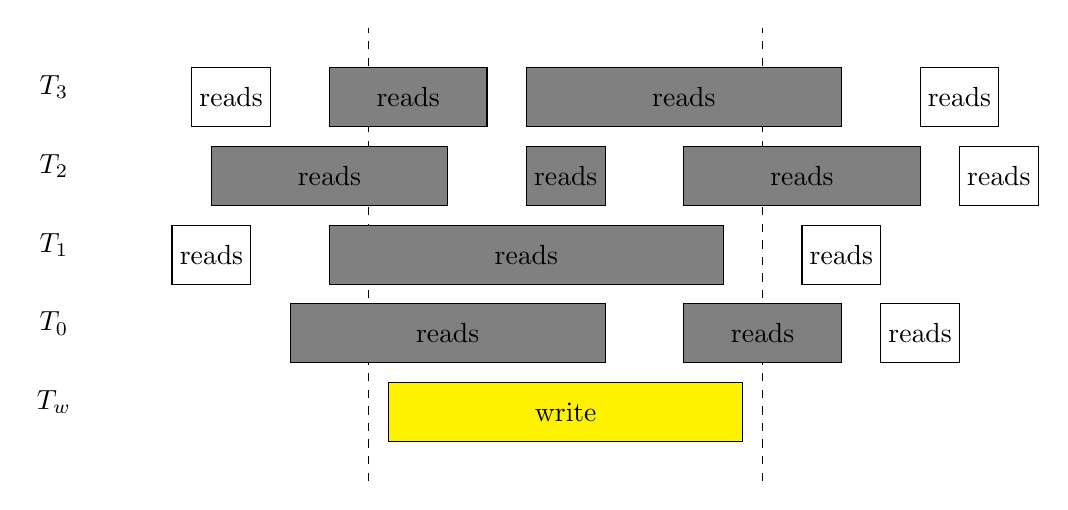
\begin{tikzpicture}
  \foreach \i in {0, 1, 2, 3} {
    \node at (-1, 0.5 + \i)  {$T_\i$};
  }
  \node at (-1, -0.5)  {$T_w$};
  \draw[dashed] (3, -1.5) -- +(0, 5.75);
  \draw[dashed] (8, -1.5) -- +(0, 5.75);

  % lectures avant
  \draw[fill=white] (0.5, 1) rectangle node {reads} +(1, 0.75);
  \draw[fill=white] (0.75, 3) rectangle node {reads} +(1, 0.75);  
  
  % lecture échouent 
  \draw[fill=gray] (2, 0) rectangle node {reads} +(4, 0.75);
  \draw[fill=gray] (2.5, 1) rectangle node {reads} +(5, 0.75);
  \draw[fill=gray] (1, 2) rectangle node {reads} +(3, 0.75);
  \draw[fill=gray] (2.5, 3) rectangle node {reads} +(2, 0.75);
  \draw[fill=gray] (7, 0) rectangle node {reads} +(2, 0.75);
  \draw[fill=gray] (5, 2) rectangle node {reads} +(1, 0.75);
  \draw[fill=gray] (7, 2) rectangle node {reads} +(3, 0.75);
  \draw[fill=gray] (5, 3) rectangle node {reads} +(4, 0.75);

  % lectures après
  \draw[fill=white] (9.5, 0) rectangle node {reads} +(1, 0.75);  
  \draw[fill=white] (8.5, 1) rectangle node {reads} +(1, 0.75);
  \draw[fill=white] (10.5, 2) rectangle node {reads} +(1, 0.75);  
  \draw[fill=white] (10, 3) rectangle node {reads} +(1, 0.75);

  % thread écrivain
  \draw[fill=yellow] (3.25, -1) rectangle node[] {write} +(4.5, 0.75);
\end{tikzpicture}


Ce mécanisme garantit qu'aucun processus d'écriture n'a eu lieu, ni n'est en
cours pendant une RSCS qui a pu être validée. Par conséquent, les écritures et
les RSCS validées sont séquentiellement consistantes.  Au passage, si un lecteur
trouve un numéro de version impair à l'entrée de la RSCS, il peut décider
d'attendre que l'écriture soit terminée.

L'avantage principal de ce mécanisme, outre sa simplicité, est que le surcoût
pour les lecteurs est très faible en l'absence de conflit. Les processus qui
modifient la structure de donnée n'ont pas non plus besoin d'attendre. Par
contre, l'inconvénient c'est que les écrivains ont la priorité sur les
lecteurs. S'il y a trop d'écrivains, les lecteurs ne pourront jamais effectuer
de lecture cohérente et auront du mal à progresser (phénomène de
\emph{livelock}).

\section{Le paradigme \emph{Read-Copy-Update} (RCU)}

Pour éviter que les lecteurs ne puissent accéder à une structure de donnée en
cours de modification, une possibilité consiste à 1) effectuer une copie de la
structure, 2) modifier la structure, 3) remplacer l'ancienne structure par la
nouvelle de façon atomique (en changeant un pointeur par exemple). Ceci peut
rappeler le fonctionnement des langages fonctionnels (toutes les données sont
\og en lecture seule\fg{}). Évidemment, ceci marche mieux avec des structures où
la modification est facile, style liste chaînée.

Au début de chaque section critique de lecture, il faut récupérer la dernière
version de la structure de donnée (par exemple en relisant le pointeur). Pour
éviter que deux écrivains ne s'exécutent en même temps, il suffit de mettre en
place une section critique.

Le problème, c'est qu'il faut bien libérer la mémoire occupée par les anciennes
versions, mais il ne faut pas le faire trop tôt, car elles peuvent être encore
en cours de lecture. Les techniques de RCU permettent de le faire au bon moment,
et peuvent être vues comme une forme de \emph{garbage collection}.

Lorsqu'un thread n'est pas dans une section critique de lecture, alors il est
\emph{tranquille} (\emph{quiescent}). S'il reste tranquille longtemps, alors on
parle d'état tranquille étendu. Un intervalle de temps dans lequel \emph{tous}
les threads passent dans un état tranquille au moins une fois est appelé une
\emph{période de grâce} (\emph{grace period}).

L'idée générale est la suivante : on accède à une structure de donnée via un
pointeur partagé ; un thread écrivain prépare une nouvelle version et la modifie
le pointeur partagé ; si une période de grâce s'écoule, alors plus aucun autre
thread ne peut encore avoir accès à l'ancienne version.

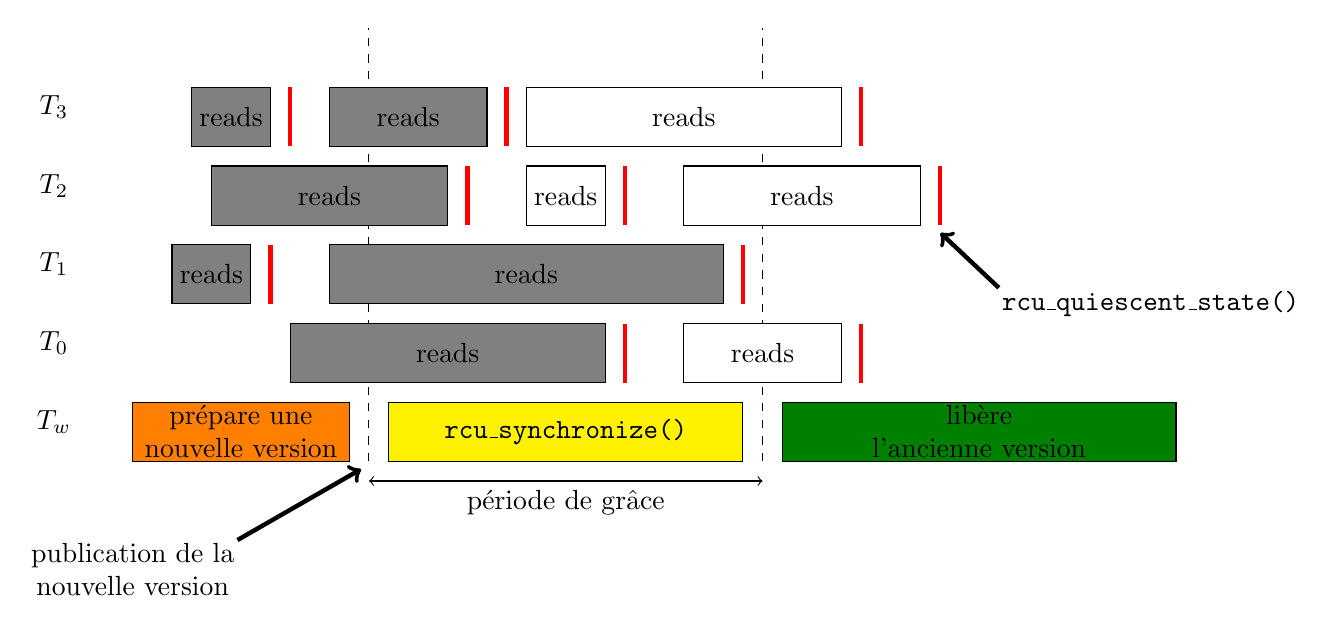
\begin{tikzpicture}
  \foreach \i in {0, 1, 2, 3} {
    \node at (-1, 0.5 + \i)  {$T_\i$};
  }
  \node at (-1, -0.5)  {$T_w$};
  \draw[dashed] (3, -1) -- +(0, 5.5);
  \draw[dashed] (8, -1) -- +(0, 5.5);

  
  % lecture anciennes
  \draw[fill=gray] (2, 0) rectangle node {reads} +(4, 0.75);
  \draw[red,ultra thick] (6.25, 0) -- +(0, 0.75);
  
  \draw[fill=gray] (0.5, 1) rectangle node {reads} +(1, 0.75);
  \draw[red,ultra thick] (1.75, 1) -- +(0, 0.75);

  \draw[fill=gray] (2.5, 1) rectangle node {reads} +(5, 0.75);
  \draw[red,ultra thick] (7.75, 1) -- +(0, 0.75);

  \draw[fill=gray] (1, 2) rectangle node {reads} +(3, 0.75);
  \draw[red,ultra thick] (4.25, 2) -- +(0, 0.75);

  \draw[fill=gray] (0.75, 3) rectangle node {reads} +(1, 0.75);
  \draw[red,ultra thick] (2, 3) -- +(0, 0.75);

  \draw[fill=gray] (2.5, 3) rectangle node {reads} +(2, 0.75);
  \draw[red,ultra thick] (4.75, 3) -- +(0, 0.75);

  % lecture nouvelles
  \draw[fill=white] (7, 0) rectangle node {reads} +(2, 0.75);
  \draw[red,ultra thick] (9.25, 0) -- +(0, 0.75);

  \draw[fill=white] (5, 2) rectangle node {reads} +(1, 0.75);
  \draw[red,ultra thick] (6.25, 2) -- +(0, 0.75);

  \draw[fill=white] (7, 2) rectangle node {reads} +(3, 0.75);
  \draw[red,ultra thick] (10.25, 2) -- +(0, 0.75);

  \draw[fill=white] (5, 3) rectangle node {reads} +(4, 0.75);
  \draw[red,ultra thick] (9.25, 3) -- +(0, 0.75);

  % thread écrivain
  \draw[fill=orange] (0, -1) rectangle node[align=center] {prépare une \\ nouvelle version} +(2.75, 0.75);
  \draw[fill=yellow] (3.25, -1) rectangle node[font=\ttfamily] {rcu\_synchronize()} +(4.5, 0.75);
  \draw[fill=Green] (8.25, -1) rectangle node[align=center] {libère \\ l'ancienne version} +(5, 0.75);
  
  % commentaires en dessous
  \draw[<->] (3, -1.25) -- node[below] {période de grâce} +(5, 0);
  \node[anchor=north, align=center, inner sep=1pt] at (0, -2)  (pub) {publication de la \\ nouvelle version};
  \draw[->, ultra thick] (pub.north east)  to (2.9, -1.1);

  % commentaire haut droite
  \node[anchor=west, inner sep=1pt] at (11, 1)  (quiet) {\texttt{rcu\_quiescent\_state()}};
  \draw[->, ultra thick] (quiet.north west)  to (10.26, 1.9);
\end{tikzpicture}

Il suffit donc d'attendre une période de grâce, et le tour est joué. Les
écrivains disposent d'une fonction \texttt{rcu\_synchronize()} qui les bloque
jusqu'à ce qu'une période de grâce se soit entièrement écoulée. De manière
alternative, les écrivains ne sont pas obligés de bloquer ; ils peuvent ajouter
la tâche qui consiste à libérer l'ancienne version de la structure de donnée à
une file d'attente ; périodiquement (s'il manque de la mémoire par exemple), un
thread peut attendre une période de grâce, puis exécuter toutes les tâches en
attente d'un seul coup.

Le problème consiste à détecter les périodes de grâce. On présente ici la
solution la plus agressive possible : pour entrer dans une section critique de
lecture, il suffit de ne rien faire du tout. Lorsqu'un thread est
\emph{tranquille}, il faut qu'il appelle la fonction
\texttt{rcu\_quiescent\_state()} périodiquement (en fait, les sections critiques
de lecture s'étendent entre deux appels à cette fonction). Si un thread va
entrer une période de tranquillité étendue, alors il peut invoquer
\texttt{rcu\_thread\_offline()}, puis \texttt{rcu\_thread\_online()} quand il va
reprendre une activité.

Bien sûr, il ne faut pas conserver de pointeur vers la structure de donnée
partagée au-delà d'un appel à \texttt{rcu\_quiescent\_state()}, car ce dernier
autorise éventuellement la libération de l'espace mémoire en question.

Une implantation possible est décrite ci-dessous. Un seul thread peut invoquer
\texttt{rcu\_synchronize} simultanément, si bien que les \og
synchronisations\fg{} peuvent être numérotées. C'est d'ailleurs à ça que sert la
variable \texttt{gc}. Il y a aussi un tableau partagé \texttt{rc}, avec une
entrée par thread, qui indique le numéro de la dernière synchronisation
effectuée lorsque ce thread était tranquille. Un thread hors-ligne indique zéro.

Pour effectuer la synchronisation, il suffit d'incrémenter \texttt{gc}, puis
d'attendre que tous les threads aient \og vu\fg{} l'incrémentation en ayant
appelé \texttt{rcu\_quiescent\_state()}.

\begin{tabular}{c|c}
\begin{minipage}[t]{0.35\textwidth}
\begin{minted}[fontsize=\small]{C}
int tid = omp_get_num_thread();
int N = omp_get_max_threads();
int gc = 1;                      
int rc[N];  // 0 initialement

void rcu_quiescent_state()
{
        #pragma omp atomic write
        rc[tid] = gc;
}

void rcu_thread_offline()
{
        #pragma omp atomic write
        rc[tid] = 0;
}

void rcu_thread_online()
{
        #pragma omp atomic write
        rc[tid] = gc;
}
\end{minted}
\end{minipage}
&
\begin{minipage}[t]{0.6\textwidth}
\begin{minted}[fontsize=\small]{C}
void rcu_synchronize()
{
        bool was_online = (rc[tid] > 0);
        if (was_online)
                rcu_thread_offline();
        #pragma omp critical
        {
                #pragma omp atomic update
                gc++;
                for (int i = 0; i < N; i++)
                       while (true) {
                                int s;
                                #pragma omp atomic read
                                s = rc[i];
                                if (s == 0 || s == gc)
                                        break;
                       }
        }
        if (was_online)
                rcu_thread_online();
}
\end{minted}
\end{minipage}
\end{tabular}

\section{Structures de données \emph{lock-free} à base de \emph{compare-and-swap}}

L'opération \og \emph{compare-and-swap}\fg{} permet de réaliser presque tout et
n'importe quoi de manière atomique. La plupart des processeurs la supportent
directement, ou bien offrent des fonctionnalités équivalentes. Les compilateurs
permettent de l'utiliser via des pseudo-fonctions spéciales (par exemple
\texttt{\_\_sync\_val\_compare\_and\_swap} dans \texttt{gcc}). Tout ceci était
incompatible d'un compilateur à l'autre. La situation s'est améliorée avec la
parution du standard \textbf{C11} (ISO/IEC 9899:2011), qui standardise tout ceci
et offre une interface standard pour \emph{compare-and-swap}.

Au passage, \OMP l'offre dans la version 5.1 de la spécification (novembre 2020)
via \texttt{\#pragma omp atomic compare}, mais en \the\year\xspace aucun compilateur ne
l'implante encore.

Dans \textsf{C11}, le nouveau fichier d'en-tête \texttt{stdatomic.h} offre alors
les fonctions :
\begin{minted}{C}
bool atomic_compare_exchange_strong(volatile A* obj, C* expected, C desired);
bool atomic_compare_exchange_weak(volatile A *obj, C* expected, C desired);
\end{minted}

Dans cette spécification (qui utilise le mécanisme de généricité de C11),
\texttt{A} est un type atomique, tandis que \texttt{C} désigne sa version
non-atomique. Les deux fonctions sont à peu près équivalentes à :
\begin{minted}{C}
bool ok = (*obj == expected);
if (ok)
        *obj = desired;
return ok;
\end{minted}
Mais tout ceci s'exécute de manière atomique. La différence entre les deux
versions consiste en ce que la version \emph{weak} peut renvoyer des faux
négatifs (c.a.d. renvoyer \texttt{false} et ne pas faire la mise-à-jour alors
que \texttt{obj} a bien la valeur \texttt{expected}). Sur certaines plate-forme,
la version \emph{weak} peut être plus rapide.

La puissance de l'opération \emph{compare-and-swap} (CAS) vient de son caractère
très générique. Cela permet de 1) lire une variable, 2) calculer une nouvelle
valeur, 3) \emph{si la variable n'a pas été modifiée entre-temps}, écrire la
nouvelle valeur. Si ça a raté, on peut recommencer. C'est la technique de la
\emph{compare-and-swap loop}.

Par exemple, on peut effectuer $n \gets n \times n$ de manière atomique (ce que ne
permet pas \texttt{\#pragma omp atomic})~:
\begin{minted}{C}
#include <stdbool.h>
#include <stdatomic.h>
  
atomic_int n;
  
while (true) {
        int snapshot = atomic_load(&n);
        int new = n * n;   // on aurait pu calculer un truc arbitraitement compliqué
        if (atomic_compare_exchange_weak(&n, &snapshot, new))
                break;
}
\end{minted}

Jusque-là, on a vu des mécanismes qui permettent aux lecteurs et aux écrivains
de cohabiter, mais les écrivains utilisaient entre eux un système d'exclusion
mutuelle. Si un écrivain restait bloqué dans la section critique, il coince tous
les autres. \textit{A contrario}, les techniques à base de \emph{CAS loop}
permettent d'éviter d'avoir à placer les écrivains dans des sections
critiques. Ceci peut aboutir à des algorithmes \emph{lock-free} : non seulement
il n'y a aucun verrou nulle part (!), mais en plus, on a la garantie qu'à
n'importe quel moment, au moins un thread peut progresser même si tous les
autres étaient suspendus indéfiniment.

Par exemple, des threads peuvent ajouter des éléments en tête d'une liste
chaînée de manière atomique. Pour cela, il faut allouer un nouveau noeud
\texttt{new}, et le problème c'est qu'il faut réussir de manière atomique à
\begin{enumerate}
\item Mettre l'adresse de la tête de la liste (\texttt{head}) dans
  \texttt{new->next}, puis
\item écrire l'adresse de \texttt{new} dans la variable qui contient l'adresse
  de la tête de la liste,
\end{enumerate}

\medskip

L'opération CAS permet de réaliser ceci. Voici un exemple d'implantation en
\textsf{C11}. Les lecteurs invoquent \mintinline{C}{read_access()} pour obtenir
un pointeur vers la tête de la liste, et tout le monde peut appeler
\mintinline{C}{atomic_push()} n'importe quand.

\begin{minted}{C}
struct item_t {
    void * data;
    struct item_t *next;
};

// pointeur atomique vers un objet normal (et non pointeur normal vers un objet atomique)
struct item_t * _Atomic head;    

const struct item_t * read_access()
{
        /*
        * sur beaucoup de processeurs, dont les x86, pour des types de base, atomic_load()
        * ne fait rien de spécial, c'est une lecture normale depuis la mémoire, qui est
        * ``nativement'' atomique.
        */
        return atomic_load(&head);
}

void atomic_push(void * payload)
{
        struct item_t *new = malloc(sizeof(*new));
        new->data = payload;
        bool ok = false;
        while (!ok) {
                new->next = atomic_load(&head);
                ok = atomic_compare_exchange_weak(&head, &new->next, new);
        }
}
\end{minted}

Le problème principal que pose l'utilisation de \emph{compare-and-swap}, c'est
que le programmeur est exposé à l'infâme problème A--B--A :
\begin{enumerate}
\item Un thread $T_0$ prend un \emph{snapshot} d'une variable partagée (valeur $A$).
\item Un autre thread $T_1$ modifie la variable partagée, qui prend la valeur $B$.
\item Un autre thread $T_2$ remodifie la variable partagée, qui \emph{reprend la valeur $A$}.
\item $T_0$ effectue un CAS pour mettre à jour la variable, et l'opération réussit à tort.
\end{enumerate}
\medskip

Il y a des techniques générales pour éviter le problème ABA, qui sont hors du
cadre de ce document. Mais il faut noter que le problème ABA ne se pose pas si
la variable partagée varie de manière monotone (ne fait qu'augmenter, on ne fait
qu'enfiler des noeuds, etc.).

\subsection{Exemple avancé : un ensemble d'entiers \emph{lock-free}}

On veut implanter une structure de donnée permettant de représenter des
sous-ensembles de $\{0, 1, 2, \dots, N-1\}$. On initialise la structure avec
l'ensemble qui contient tous les entiers inférieurs à $N$. On veut pouvoir
déterminer si l'ensemble est vide, extraire son minimum, et en retirer un
élément arbitraire, le tout \emph{en temps constant amorti}. Séquentiellement,
ceci est facile avec un tableau de booléens. (On pourrait aussi le faire avec
une liste doublement chaînée, et alors ce serait en temps constant dans le pire
des cas).

\begin{tabular}{c|c}
\begin{minipage}[t]{0.5\textwidth}
\begin{minted}[fontsize=\small]{C}
bool * A;
int N;
int min;

void setup()
{
	A = malloc((N + 1) * sizeof(*A));
	for (int i = 0; i < N + 1; i++)
		A[i] = true;
        min = 0;
}
\end{minted}
\end{minipage}
  &
\begin{minipage}[t]{0.6\textwidth}
\begin{minted}[fontsize=\small]{C}
bool remove(int i)
{
        bool prev = A[i];
        A[i] = false;
        return prev;
}

int extract_min()
{
        while(A[min] == false)
                min++;
        if (min < N)
                remove(min);
	return min;
}
\end{minted}
\end{minipage}
\end{tabular}

\medskip

La fonction \texttt{remove} renvoie \texttt{true} si l'élément retiré était bien
présent dans l'ensemble. La fonction \texttt{extract\_min} renvoie $N$ lorsque
l'ensemble est vide. Le principal invariant de la structure de donnée est le
suivant : \texttt{A[i] == false} pour $0 \leq i < \texttt{min}$. Comme
\texttt{A[N] == true}, la boucle \texttt{while} ne peut pas entraîner un accès
au-delà de la taille allouée pour \texttt{A}.

La fonction \texttt{extract\_min} s'exécute en temps constant amorti : pour
chaque \texttt{remove()} qui a lieu, on met 1\euro de côté et on le laisse sur
la case en question. Chaque itération de la boucle \texttt{while} consomme
l'euro trouvé sur la case sautée. On ne passe jamais à découvert.

Pour rendre le tout \emph{thread-safe} et \emph{lock-free}, on laisse
\texttt{remove()} tel quel, par contre il faut changer
\texttt{extract\_min()}. En effet, on peut parcourir le tableau jusqu'à trouver
une case \texttt{true}, mais elle peut changer \og sous nos pieds\fg{} si un
autre \texttt{extract\_min()} a lieu en même temps. Heureusement, on peut
obtenir un effet atomique avec un \emph{compare-and-swap}.

\begin{tabular}{c|c}
\begin{minipage}[t]{0.42\textwidth}
\begin{minted}[fontsize=\small]{C}
atomic_bool * A;
int N;
atomic_int min;
bool yes = true;

#define CAS atomic_compare_exchange_weak

void setup()
{
	A = malloc((N + 1) * sizeof(*A));
	for (int i = 0; i < N + 1; i++)
		atomic_store(&A[i], true);
        atomic_store(&min, 0);
}

bool remove(int i)
{
	atomic_exchange(&A[i], false);
}
\end{minted}
\end{minipage}
  &
\begin{minipage}[t]{0.58\textwidth}
\begin{minted}[fontsize=\small]{C}
int extract_min()
{
        int old = atomic_load(&min);
        int i = old;
        while(atomic_load(&A[i]) == false)
                i++;
        if (i < N) {
                bool ok = CAS(&A[i], &yes, false);
                if (!ok)
                        // raté : on recommence
                        return extract_min();
        }
        // ici, on sait que soit l'ensemble est vide (i == N)
        // soit on a retiré i de l'ensemble. On tente de
        // faire avancer min ``paresseusement''.
        CAS(&min, &old, i);
        return i;
}
\end{minted}
\end{minipage}
\end{tabular}

En fait, vu de l'extérieur, tout se passe comme \texttt{extract\_min()} \og
prenait effet \fg{} \emph{instantanément} lorsque \texttt{ok = true}. La
fonction essaye ensuite de mettre à jour \texttt{min}, mais ceci n'est pas
critique. Au pire, ça ralentira un peu le prochain \texttt{extract\_min()}.

Il n'est pas complètement évident de garantir la correction de l'algorithme. Une
structure de donnée est \emph{linéarisable} si tout se passe comme si les
fonctions qui y accèdent prenaient effet \emph{instantanément}, à un point
quelconque entre leur invocation et leur terminaison. Pour chaque fonction, il
faut donc déterminer un ou des \emph{points de linéarisation} (où elle prend
effet \og instantanément \fg{}). Dans \texttt{extract\_min()}, cela peut être à
la sortie de la boucle \texttt{while}.

Si une structure de donnée est linéarisable, alors tout se passe comme si les
fonctions qui y accèdent étaient exécutées Séquentiellement, dans l'ordre des
points \og instantanés\fg{} où elles prennent effet. Elle doit renvoyer les
mêmes résultats dans l'exécution parallèle que dans l'exécution séquentielle
fictive. Il s'agit maintenant de démontrer que le code ci-dessus est
linéarisable.

À cette fin, on prétend que l'invariant est maintenu par la version parallèle de
la fonction. Supposons qu'il soit vrai à l'entrée de \texttt{extract\_min()}. Si
\texttt{min} est modifié, il passe de \texttt{old\_min} à \texttt{i}, et la
fonction a observé que \texttt{A[old\_min:i] == false}. Par conséquent, la
modification respecte l'invariant. Et si la modification n'a pas lieu, alors
l'invariant est encore respecté. Bilan : en sortie de la fonction, l'invariant
est maintenu.

L'invariant garantit que \texttt{extract\_min()} renvoie bien le plus petit
élément de l'ensemble : on a \texttt{A[i] == false} pour tous les
$i < \texttt{min}$, et la fonction renvoie le premier $i \geq \texttt{min}$ qui
convient. Par conséquent, on peut affirmer que \og tout se passe comme si la
fonction s'exécutait instantanément au moment où le \emph{compare-and-swap} (sur
\texttt{A[i]}) a réussi\fg{}.

\subsection{Exemple (plus) avancé : une file non-bornée \emph{lock-free}}

Les algorithmes \emph{lock-free} sont difficiles en général. L'un des plus
simples est le suivant. On considère une file (FIFO), munie de deux fonctions
\texttt{enqueue()} et \texttt{dequeue()}. Le tout est implanté avec une liste
simplement chaînée. On conserve deux pointeurs vers la tête et la queue de la
liste. Les éléments sont ajoutés à la queue et prélevés à la tête. Il y a
toujours un noeud \og sentinelle\fg{} inutilisé à la tête de la liste.

Une implantation (bloquante) possible est la suivante. On remarque que deux
threads différents peuvent exécuter \texttt{enqueue()} et \texttt{dequeue()}
simultanément, car les sections critiques ont des noms différents. De plus, les
deux fonctions ne sont pas en conflit.

\begin{tabular}{c|c}
\begin{minipage}[t]{0.48\textwidth}
  \begin{minted}[fontsize=\small]{C}
struct node_t {
	void * data;
	struct node_t * next;
};


struct node_t * head;
struct node_t * tail;


void setup()
{
	struct node_t * sentinel = 
		malloc(sizeof(*sentinel));
	sentinel->data = NULL;
	sentinel->next = NULL;
	head = sentinel;
	tail = sentinel;
}
\end{minted}
\end{minipage}
&
\begin{minipage}[t]{0.48\textwidth}
\begin{minted}[fontsize=\small]{C}
void enqueue(void * payload)
{
	assert(payload != NULL);
	struct node_t * node = malloc(sizeof(*node));
	node->data = payload;
	#pragma omp critical (enqueue)
	{
                assert(tail->next == NULL);
		tail->next = node;
		tail = node;
	}
}

void * dequeue()
{
	void * result = NULL;
	#pragma omp critical (dequeue)
	{
		struct node_t * next = head->next; 
		if (next != NULL) {
			result = next->data;
			free(head);
			head = next;
		}
	}
	return result;
}
\end{minted}
\end{minipage}
\end{tabular}

Enfiler un nouveau noeud fonctionne en deux phases : $i$) faire pointer le
dernier noeud vers le nouveau noeud, puis $ii$) avancer \texttt{tail} vers le
nouveau noeud.

Défiler un noeud fonctionne en trois phases : $i$) vérifier si \texttt{head !=
  NULL}, puis $ii$) le cas échéant, avancer \texttt{head} vers le noeud
suivant. Enfin, une fois que c'est fait, on peut $iii$) récupérer le champ
\texttt{data} de l'ex-premier noeud, puis le désallouer.

Pour défiler, on pourrait :
\begin{enumerate}
\item Récupérer $\texttt{first} \gets \texttt{head}$.
\item Récupérer $\texttt{next} \gets \texttt{first->next}$.
\item Faire un compare-and-swap pour avancer \texttt{head} vers \texttt{next}, à condition que rien n'ait changé depuis le début, donc que \texttt{head == first}.
\item (à ce moment-là, \texttt{first} est inaccessible aux autres threads). Lire
  les données dans \texttt{first} puis désallouer \texttt{first}.
\end{enumerate}  

Le problème pour enfiler un noeud, c'est qu'on ne va pas pouvoir faire les
étapes $i$ et $ii$) de façon atomique, donc si plusieurs threads essayer
d'enfiler en même temps, il peut se trouver une situation où ils ont tous fait
l'étape $i$), mais aucun n'a fait l'étape $ii$). Par conséquent, il va se
trouver des moments où \texttt{tail} peut \og être en retard\fg{}, c'est-à-dire
pointer sur un noeud qui a un successeur.

Quand un thread rencontre cette situation, deux options seraient possibles :
\begin{enumerate}
\item Attendre que l'autre thread qui est en train de modifier la structure de données ait fini.
\item L'aider en faisant son travail à sa place.
\end{enumerate}
\medskip

Le seul moyen d'être \emph{lock-free} est la deuxième solution. Pour pouvoir
effectuer \emph{compare-and-swap}, on utilise encore des pointeurs atomiques
pour \texttt{head}, \texttt{tail} et les champs \texttt{next} de tous les
noeuds. Voici les préliminaires :

\begin{minted}[fontsize=\small]{C}
#include <stdatomic.h>
	
struct node_t {
	void * data;
	struct node_t * _Atomic next;
};

struct node_t * _Atomic head;
struct node_t * _Atomic tail;

struct node_t * make_node(void * payload)
{
	struct node_t * node = malloc(sizeof(*node));
	assert(node != NULL);
	node->data = payload;
	atomic_store(&node->next, NULL);
	return node;
}

void setup()
{
	struct node_t * sentinel = make_node(NULL); 
	atomic_store(&head, sentinel);
	atomic_store(&tail, sentinel);
}
\end{minted}

La fonction \texttt{enqueue}() récupère \texttt{tail} et observe le champ
\texttt{next} du noeud en question. S'il n'est pas \texttt{NULL}, c'est que \og
\texttt{tail} est en retard\fg{}. On commence par essayer de réparer
\texttt{tail} avant toute chose. Après, on utilise un CAS pour essayer de faire pointer de manière atomique

\begin{minted}[fontsize=\small]{C}
void enqueue(void * payload)
{
	assert(payload != NULL);
	struct node_t * node = make_node(payload);
	while (true) {
		struct node_t * last = atomic_load(&tail);
		struct node_t * next = atomic_load(&last->next);
		if (next != NULL) {              
			// tail a un successeur ?!? Un autre enqueue() est en cours et pas terminé.
			// Je vais l'aider ! D'abord on fait avancer tail, puis on ressaye d'enfiler.
			atomic_compare_exchange_weak(&tail, &last, next);
			continue;
                }
		// i) Mettre à jour le champ next du dernier noeud, si rien n'a changé depuis le début
		bool ok = atomic_compare_exchange_weak(&last->next, &next, node);
		if (!ok)
			continue;  // raté: un autre enqueue() nous a doublé et a rajouté un noeud à la fin.
		// ii) fait avancer tail vers le nouveau noeud (pas grave si ça rate, les autres répareront)
		atomic_compare_exchange_weak(&tail, &last, node);
		return;
	}
}
\end{minted}

Si la variable \texttt{ok} passe à vrai, alors le nouveau noeud est ajouté à la
file, et tous les autres threads peuvent alors le voir. Par contre,
\texttt{tail} peut ne pas être mis à jour correctement, par exemple si quelqu'un
a décidé de nous \og aider\fg{} entre l'étape $i$) et l'étape $ii$).

\texttt{dequeue} fonctionne à peu près de la même façon, mais il faut se
préparer à aider un éventuel \texttt{enqueue} qui ajouterait le premier noeud.

\begin{minted}[fontsize=\small]{C}
void * dequeue()
{
	while (true) {
		struct node_t * first = atomic_load(&head); 
		struct node_t * last = atomic_load(&tail);
		struct node_t * next = atomic_load(&first->next); 
                // i) vérifier si la file est vide
                if (first == last) {
			// La file a l'air vide...
			if (next == NULL)
				return NULL; // ... et elle est vraiment vide
			// tail a un successeur ? Un enqueue() a ajouté un premier noeud, et n'est pas terminé.
			// Je vais l'aider ! On essayer d'avancer tail, puis on réessaye de défiler.
			atomic_compare_exchange_weak(&tail, &last, next);
			continue;
		}
		// ii) Faire pointer head sur le noeud suivant
		bool ok = atomic_compare_exchange_weak(&head, &first, next);
		if (!ok)
			continue; // Raté : un autre dequeue() a changé head ; first est périmé  
                // iii) On peut faire ce qu'on veut avec le noeud défilé
                void * payload = next->data;
		// free(first);  // WARNING : triggers ABA problem
		return payload;
	}
}
\end{minted}

On déduit de \texttt{first != last} que la file n'est pas vide, donc en
particulier que \texttt{next != NULL}. Ceci fonctionne correctement, mais
\emph{seulement} parce qu'on lit \texttt{tail} avant de lire
\texttt{first->next}. Ceci est subtil. En effet, si on avait écrit :
\begin{minted}{C}
struct node_t * first = atomic_load(&head); 
struct node_t * next = atomic_load(&first->next); 
struct node_t * last = atomic_load(&tail);
\end{minted}
Alors le problème suivant pourrait avoir lieu :
\begin{enumerate}
\item La file est vide.
\item On lit \texttt{head}, puis \texttt{first->next == NULL}
\item À Ce moment-là, quelqu'un ajoute un noeud, fait avancer \texttt{tail}, et on se retrouve avec \texttt{head != tail}.
\end{enumerate}
Si on laissait faire ceci, alors on pourrait accidentellement retirer le noeud sentinelle, et la file serait cassée.

Un autre problème subtil est que ceci est vulnérable au problème ABA, à cause de
\texttt{malloc} et de \texttt{free}. En effet, une fois qu'un noeud est libéré,
\texttt{malloc} peut potentiellement renvoyer la même adresse.


La séquence d'évènements problématique est la suivante.
\begin{enumerate}
\item $T_0$ lance \texttt{dequeue()}; la file n'est pas vide; il s'apprête à faire un \emph{compare-and-swap} qui fera $\texttt{head} \gets b$ si $\texttt{head} = a$ (cf. figure).
\item Juste à ce moment-là, $T_1$ effectue lui aussi deux \texttt{dequeue()} qui s'exécutent entièrement. $a$ et $b$ sont libérés.
\item Un \texttt{enqueue()} a lieu. L'adresse du noeud $a$ est renvoyée par \texttt{malloc} ; un nouveau noeud de la file possède donc l'adresse $a$.
\item Plusieurs \texttt{dequeue()} ont lieu, et le noeud $a$ se retrouve en position de sentinelle ; \texttt{head} pointe dessus.
\item Le thread $T_0$ se réveille et effectue son \emph{compare-and-swap} ; il réussit car $\texttt{head} = a$, mais il affecte incorrectement la valeur $b$ à \texttt{head}, ce qui casse la liste.
\end{enumerate}

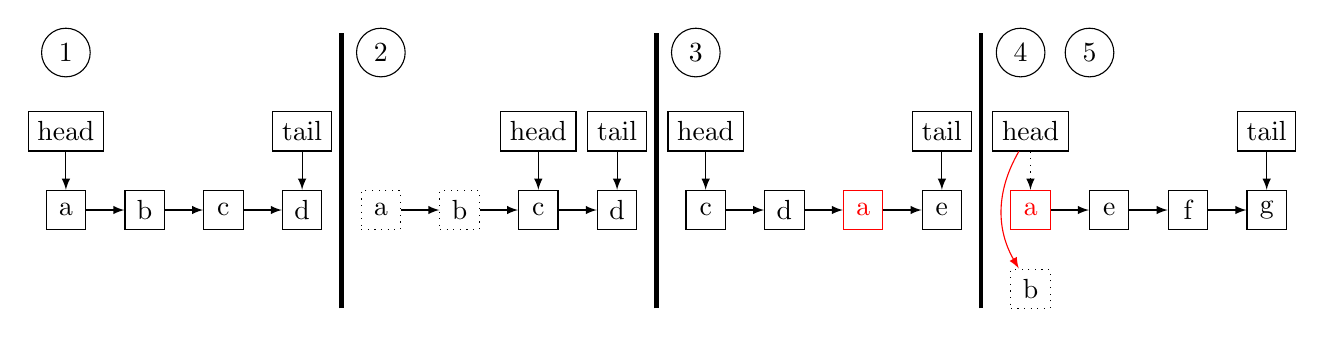
\begin{tikzpicture}[scale=0.5,every node/.style={minimum height=5mm, minimum width=5mm},>=latex]
  \node[draw] at (0, 2) (head) {head};
  \node[draw] at (6, 2) (tail) {tail};

  \node[draw] at (0, 0) (a) {a};
  \node[draw] at (2, 0) (b) {b};
  \node[draw] at (4, 0) (c) {c};
  \node[draw] at (6, 0) (d) {d};
  
  \draw (head) edge[->] (a);
  \draw (tail) edge[->] (d);

  \draw (a) edge[->] (b);
  \draw (b) edge[->] (c);
  \draw (c) edge[->] (d);

  \draw[ultra thick] (7, -2.5) -- +(0, 7);
  \draw[ultra thick] (15, -2.5) -- +(0, 7);
  \draw[ultra thick] (23.25, -2.5) -- +(0, 7);

  \node[draw,shape=circle] at (0, 4)  {1};
  \node[draw,shape=circle] at (8, 4)  {2};
  \node[draw,shape=circle] at (16, 4) {3};
  \node[draw,shape=circle] at (24.25, 4)  {4};
  \node[draw,shape=circle] at (26, 4)  {5};
  
  
  \begin{scope}[xshift=8cm]
\node[draw] at (4, 2) (head) {head};
  \node[draw] at (6, 2) (tail) {tail};

  \node[draw,dotted] at (0, 0) (a) {a};
  \node[draw,dotted] at (2, 0) (b) {b};
  \node[draw] at (4, 0) (c) {c};
  \node[draw] at (6, 0) (d) {d};
  
  \draw (a) edge[->] (b);
  \draw (b) edge[->] (c);

  \draw (head) edge[->] (c);
  \draw (tail) edge[->] (d);

  \draw (c) edge[->] (d);
\end{scope}

  
  \begin{scope}[xshift=12.25cm]
  \node[draw] at (4, 2) (head) {head};
  \node[draw] at (10, 2) (tail) {tail};

  \node[draw] at (4, 0) (c) {c};
  \node[draw] at (6, 0) (d) {d};
  \node[draw,red] at (8, 0) (a) {a};
  \node[draw] at (10, 0) (e) {e};

  \draw (head) edge[->] (c);
  \draw (tail) edge[->] (e);

  \draw (c) edge[->] (d);
  \draw (d) edge[->] (a);
  \draw (a) edge[->] (e);
\end{scope}

  \begin{scope}[xshift=16.5cm]
    \node[draw] at (8, 2) (head) {head};
    \node[draw] at (14, 2) (tail) {tail};

    \node[draw,dotted] at (8, -2) (b) {b};
    
    \node[draw,red] at (8, 0) (a) {a};
    \node[draw] at (10, 0) (e) {e};
    \node[draw] at (12, 0) (f) {f};
    \node[draw] at (14, 0) (g) {g};
    
    \draw (head) edge[->,dotted] (a);
    \draw (head) edge[->,red,bend right] (b);
    
    \draw (tail) edge[->] (g);
    
    \draw (a) edge[->] (e);
    \draw (e) edge[->] (f);
    \draw (f) edge[->] (g);
  \end{scope}
\end{tikzpicture}

Peut-on éviter le problème ABA ? Une technique classique consiste à
\emph{versioner} les pointeurs, c'est-à-dire à associer à chaque pointeur un
entier (son numéro de version). Chaque fois qu'une nouvelle valeur est affectée
à un pointeur, le numéro de version est incrémenter. Sur une architecture
64-bits, cela signifie que les pointeurs vont faire 128 bits. La plupart des
architectures 64-bits ont ou bien des instructions \emph{compare-and-swap} 128
bits, ou bien des instructions \emph{load-linked / store conditional} qui ne
sont pas sujette au problème ABA. Par contre, ça complique un peu le code, et
surtout \texttt{gcc} n'utilise pas directement ces instructions, ce qui ralentit
beaucoup les choses.

%TODO : hardware transactionnal memory : TSX, BG/Q...

%exercices : MCAS from CAS

\section*{Notes}

Le mécanisme de \emph{versioning} décrit ici est classique ; il est tiré de la
documentation du noyau
linux\footnote{\url{https://www.kernel.org/doc/Documentation/locking/seqlock.rst}}. Le
mécanisme de RCU décrit ici est issu de~\cite{DesnoyersMSDW12} ; il est
abondamment utilisé dans le noyau Linux lui aussi. La file \emph{lock-free} présentée ici est
tirée de~\cite{MichaelS96}.


\chapter{La vectorisation}
\label{chap:vectorization}

\section{Introduction}

VRAC : loop unrolling
VRAC : vectorisation FFT, \og 6-step algorithm\fg, radix de la taille des vecteurs

\url{https://ce-publications.et.tudelft.nl/publications/47_vector_processor_customization_for_fft.pdf}


Ce qu'on appelle la \og \emph{vectorisation}\fg est à la fois une manière
algorithmique de raisonner et une technique de programmation ; en huit mots, il
s'agit d'effectuer des opérations sur des \emph{vecteurs}, et en particulier sur
de \emph{longs} vecteurs. Il y a plusieurs idées sous-jacentes.

\subsection{Exprimer le parallélisme de données}

Les opérations sur les vecteurs sont trivialement parallélisables, et plus les
vecteurs utilisés sont longs, plus il y a de parallélisme à
exploiter. Considérons par exemple $\vec u \gets \vec u + \alpha \vec v$, où $u$
et $v$ sont des vecteurs de taille $n$ tandis que $\alpha$ est un scalaire. On
peut écrire :
\begin{minted}{C}
for (int i = 0; i < n; i++)
    u[i] = u[i] + alpha * v[i];
\end{minted}
Les itérations de la boucle ne sont pas en conflit les unes avec les autres, et
le tout est facile à paralléliser. Le langage \textsf{Fortran
  90}\footnote{Enfin, il a quand même fallu attendre 1990 pour avoir droit à des
  noms de fonctions de plus de 6 caractères...} introduit des opérations sur des
vecteurs, ce qui permet d'écrire directement \mintinline{fortran}{U = U + alpha*V}.
Il y a aussi la possibilité de faire de l'\emph{adressage indirect}, ce qui
augmente grandement les possibilités d'écriture d'algorithmes vectoriels : on
peut écrire \mintinline{fortran}{A(U) = V} ou \mintinline{fortran}{W = B(U)},
ce qui équivaut à
\begin{minted}{C}
for (int i = 0; i < n; i++) {
    A[U[i]] = V[i]; // 1er cas. Ceci n'a de sens que si U[i] != U[j]
    W[i] = B[U[i]]; // 2ème cas.
}
\end{minted}

Dans le premier cas, on parle de \og \emph{scatter}\fg (dispersion, écriture
avec adressage indirect), tandis que le deuxième cas est un \og \emph{gather}\fg
(rassemblement, lecture avec adressage indirect). Les deux opérations font
généralement souffrir le système d'accès à la mémoire et sont nettement moins
efficaces que des accès mémoires \og directs\fg (avec adresses contigües) ---
plus de détails au chapitre~\ref{chap:memory}.

En \textsf{C++} ou en \textsf{Python} on peut définir des classes qui
surchargent les opérateurs arithmétiques habituels, ce qui permet d'écrire le
même genre de chose... mais pas en \textsf{C}.


\subsection{Utiliser le matériel disponible}

Au milieu des années 1970, les machines basées sur des \emph{processeurs
  vectoriels} se sont développées et ont dominé le monde du calcul
scientifique. Cela a commencé avec le \texttt{CRAY-1} (160 MFLOPS) en 1975 ---
il s'en est vendu 80, ce qui en fait le plus grand succès commercial parmi les
machines ultra haut de gamme valant des millions de dollars). Le \texttt{CRAY-1}
a gardé la place de numéro 1 jusqu'en 1983, où il l'a cédé au... \texttt{CRAY
  X-MP/4} (713 MFLOPS) puis au \texttt{CRAY-2} (1.4 GFLOPS, 1985). Les machines
vectorielles ont tenu le haut du pavé (avec de brèves interruptions) jusqu'à
2004, où le \texttt{Earth Simulator} construit par NEC (35.6 TFLOPS) a perdu la
première place qu'il occupait depuis 2001.

Elles ont depuis été supplantées par des \anglais{clusters} assemblés à partir
de composants plus communs (processeurs largement disponibles commercialement,
GPUs, etc.) et donc moins coûteux.

Les \emph{processeurs vectoriels} qui équipent ces machines contiennent des
unités d'exécutions dédiées aux opérations sur des vecteurs. Ceci a plusieurs
avantages. Premièrement, cela permet au code de donner une grande quantité de
travail à effectuer au processeur avec une seule instruction. Du coup, moins de
temps et d'énergie sont gaspillés à décoder des instructions, gérer des
dépendances dans un pipeline, etc. Deuxièmement, comme le travail à effectuer
est largement parallélisable, le processeur peut le faire plus ou moins en
parallèle : il peut par exemple contenir $k$ circuits capable de multiplier des
flottants, et donc traiter les éléments d'un vecteur \og par paquets de $k$\fg
en parallèle (et ceci pour n'importe quelle valeur de $k$).

Un processeur normal dispose de registres pouvant contenir des scalaires
(typiquement un \texttt{double}, donc des registres de 64 bits). Un processeur
vectoriel dispose en outre de registres pouvant contenir des vecteurs,
c'est-à-dire des tableaux d'une taille fixe (typiquement de 64 à 256
\texttt{double} ; dans le dernier cas, ce sont des registres de 16384 bits).
Les opérations arithmétiques sur les vecteurs peuvent se faire entre registres
(comme dans les processeurs RISC).

Dans l'une des architectures de référence, l'IBM 370/3090 datant de
1988~\cite{PadegsMSB88}, la taille des registres vectoriels n'est même pas
spécifiée. Ceci ouvrait la voie à des processeurs moins chers avec de petits
vecteurs qui resteraient compatibles avec des processeurs plus chers munis de
grands vecteurs et de plus d'unités d'exécution. Le même exécutable doit
fonctionner correctement sur tous, sans recompilation.

Les processeurs vectoriels disposent généralement d'un registre spécial, dont la
valeur peut être lue et écrite par le programme, qui indique la taille des
vecteurs à traiter (bien sûr, elle doit être inférieure au maximum supporté par
le matériel). Ils offrent aussi généralement un système de \emph{masques}, qui
permet d'effectuer des opérations sur un sous-ensemble arbitraire des éléments
d'un vecteur. Ils offrent des instructions puissantes pour déplacer des éléments
à l'intérieur des vecteurs. Enfin, ils offrent généralement des moyens efficaces
de lire et d'écrire des vecteurs à des adresses mémoire non contiguës (accès
avec \anglais{stride}, \anglais{scatter}/\anglais{gather}, etc.). En général, il
y a des mécanismes spéciaux qui sont capables de gérer un grand nombre d'accès
mémoire simultanés (pour lire et écrire les vecteurs depuis la mémoire).

Pour exploiter un processeur vectoriel, il faut que le compilateur émette les
instructions vectorielles ; il faut donc ou bien utiliser un langage \emph{ad
  hoc} dans lequel les vecteurs soient explicités, ou bien utiliser un
compilateur \emph{vectorisant} qui détecte l'usage de vecteurs par le
programmeur et qui les réécrit en utilisation les instructions vectorielles.

\section{Instructions SIMD dans les machines \og grand public\fg}

Les processeurs largement disponibles commercialement n'ont jamais eu
d'instructions vectorielles telles que décrites ci-dessus (avec de grands
vecteurs), car leur utilisation efficace nécessite une bande passante mémoire
élevée qui n'était pas disponible dans des machines conventionnelles.

Mais depuis 1996, les processeurs grand public les plus répandus (les x86)
possèdent des instructions dites SIMD, c'est-à-dire des instructions qui
effectuent le même traitement sur plusieurs données en parallèle. Elles ont
d'abord été appelées des instructions \og multimédia\fg. En effet, elles sont
nées de l'observation que beaucoup d'applications \og multimédia\fg (avec
images, son, vidéo) manipulent des données plus petites que les 32 bits ou les
64 bits d'un mot machine. Par exemple, dans beaucoup de systèmes graphiques, 8
bits sont utilisés pour encoder chacune des trois couleurs primaires, plus
éventuellement 8 autres bits pour la transparence. Dans les traitement audio, un
échantillon est généralement codé sur 8 ou 16 bits.

Du coup, certaines de ces applications pouvaient être accélérées par des
opérations parallèles sur de petits types de données, à l'intérieur de registres
\og normaux\fg de 32 ou 64 bits. Ceci a commencé par l'ajout des instructions
MMX dans les processeurs Intel, qui utilisaient les registres flottants 64 bits
du FPU pour effectuer 4 ou 8 opérations parallèles sur des types de 16 ou 8 bits
en une seule opération. AMD a introduit un jeu d'instructions concurrent et
incompatible nommé \verb|3DNow!|, qui a été retiré en 2010 après avoir eu peu de
succès.

Ensuite, Intel a ajouté les instructions SSE, qui introduisent des registres
dédiés, plus grands (128 bits), ce qui permet plus de parallélisme. Ils ne
gèrent que les \texttt{float} (32 bits, simple précision) De nouvelles
instructions SSE ont été ajoutées régulièrement jusqu'en 2010. Le plus notable
est le SSE2, qui ajoute des opérations sur des \texttt{double} et les
entiers. Là, on est passé aux instructions AVX, qui doublent encore la taille
des registres et opèrent uniquement sur des flottants. L'AVX2 ajoute le support
des entiers et une instruction \emph{gather}. Enfin, récemment l'AVX512 a fait
sont apparition, avec des registres encore plus gros et des fonctionnalités
(masques, ajout du \emph{scatter}) qui le rapprochent des anciennes
architectures vectorielles. Voir la figure~\ref{teb:SIMD-ISA} pour un
récapitulatif.

\begin{figure}
\centering
  \begin{tabular}{|c||c|c|c|c|c|}
  \hline
  ISA & Accronyme & Nom & année & \# registres & taille des registres \\
  \hline  \hline
  \multirow{9}{*}{x86-64} & MMX & Multi Media eXtensions & 1996 & 8 & 64 \\
  \cline{2-6}
  & 3DNow! &                                            & 1998 & 8  &  64 \\
    \cline{2-6}
  & SSE    & \multirow{4}{*}{Streaming SIMD Extensions} & 1999 & \multirow{5}{*}{16} & \multirow{5}{*}{128} \\
%    \cline{2-2}
  & SSE2   &                           & 2001 &         & \\
 %   \cline{2-2}
  & SSE3   &                           & 2004 &         & \\
%    \cline{2-2}
  & SSSE3  &                           & 2004 &         & \\
%    \cline{2-2}
  & SSE4   &                           & 2007 &         & \\
    \cline{2-6}
  & AVX    & \multirow{3}{*}{Advanced Vector eXtensions} & 2010 & \multirow{2}{*}{16} & \multirow{2}{*}{256} \\
%    \cline{2-2}
  & AVX2   &                           & 2013  &    &     \\
    \cline{2-2}\cline{4-6}
  & AVX512 &                           & 2017  & 32 & 512 \\
  \hline\hline
  PowerPC & Altivec & & 1999 & 32 & 128 \\
  \hline\hline
  ARM v7 & \multirow{2}{*}{NEON} & \multirow{2}{*}{Advanced SIMD extension}    & 2005 & 16 & \multirow{2}{*}{128} \\
  \cline{1-1}%\cline{4-5}
  \multirow{2}{*}{ARM v8} &      &                            & 2011 & 32 &  \\
  \cline{2-6}
   & SVE  & Scalable Vector Extensions & 2020 & 32 & 128--2048 \\
  \hline
\end{tabular}  
\caption{Récapitulatif des principaux jeux d'instruction SIMD dans les processeurs grand public.\label{teb:SIMD-ISA}}
\end{figure}

Le problème avec ce mille-feuille, c'est qu'à la parution de chaque nouveau jeu
d'instruction, il faut non seulement mettre à jour les compilateurs, mais au
minimum recompiler les applications pour tirer partie des nouvelles
instructions. Et il faut même bien souvent \emph{réécrire} une partie du code
voire même changer des algorithmes pour vraiment tirer avantage des nouvelles
fonctionnalités. Ceci demande un effort de programmation important et nuit à la
portabilité : un exécutable qui fait appel aux \og nouvelles\fg instructions ne
peut pas fonctionner sur un processeur qui ne les implante pas. Ceci nécessite
éventuellement de détecter \emph{à l'exécution} si tel ou tel jeu d'instruction
est supporté par le processeur, et choisir en fonction différentes version du
code a exécuter.

Les raisons de la prolifération et du succès de ces instructions SIMD sont
multiples, mais on peut en retenir quelques unes : c'était assez facile et assez
peu coûteux de les ajouter à des processeurs existants; c'est un moyen facile et
simple d'augmenter sensiblement la performance de crête du processeur (son
nombre de FLOP/s); ces instructions sont difficile à utiliser directement par
les programmeurs, mais ces derniers peuvent faire appel à des bibliothèques
optimisées qui les utilisent pour effectuer le gros des calculs.

Ceci dit, on assiste peut-être à un \anglais{revival} des anciennes
architectures vectorielles : le jeu d'instructions SVE proposé par ARM (et qui
est notamment implanté sur \texttt{fugaku}, la machine qui occupe la place
n\textdegree 1 au TOP500) ressemble beaucoup ceux des anciennes machines
vectorielles. Et l'AVX512 en incorpore aussi davantage de
fonctionnalités. Enfin, l'architecture libre RISC-V propose des extensions
vectorielles qui reprennent l'architecture proposée par IBM dans les années
1980.

\section{SSE / AVX2 / AVX512 : description succincte}

Les processeurs qui supportent ces jeux d'instruction ont des registres
\og vectoriels\fg. L'AVX512 spécifie en plus des registres de masquage.

\begin{center}
\begin{tabular}{|c|c|c|}
  \hline
  Instructions & registres & taille \\
  \hline\hline
  SSE$x$              & \texttt{\%xmm0}, \dots, \texttt{\%xmm15} & 128 bits \\
  \hline
  AVX + AVX2          & \texttt{\%ymm0}, \dots, \texttt{\%ymm15} & 256 bits \\
  \hline
  \multirow{2}{*}{AVX512} & \texttt{\%zmm0}, \dots, \texttt{\%zmm31} & 512 bits \\
               & \texttt{\%k0}, \dots, \texttt{\%k7}      & 64 bits \\
  \hline
\end{tabular}
\end{center}

Ces registres sont emboîtés les uns dans les autres : \texttt{\%xmm}$i$
constitue les 128 bits de poids faible de \texttt{\%ymm}$i$, qui constitue
lui-même les 256 bits de poids faible de
\texttt{\%zmm}$i$. Cf. Figure~\ref{fig:simd-reg}.

Au passage, lorsqu'on fait des calculs non-vectorisés avec des flottants, les
compilateurs émettent des instructions qui opèrent uniquement sur la première
case des registres SSE.
\begin{danger}
  Par exemple, si on lui donne ce code à GCC:
\begin{minted}{C}
for (int i = 1; i < n; i++)
    a[i] += a[i-1];
\end{minted}
  On obtient le code assembleur suivant, qui opère sur le registre SSE \texttt{\%xmm0}, avec des instrcutions \og scalaires\fg (cf. ci-dessous).
\begin{minted}{gas}
; %rax contient l'adresse de A
; %r13 contient l'adresse de la fin de A
.loop:
        movsd   (%rax), %xmm0         ; charge A[i] dans %xmm0[0]
        addsd   -8(%rax), %xmm0       ; additionne A[i-1] à %xmm0[0]
        addq    $8, %rax              ; avance le pointeur de 8 octets
        movsd   %xmm0, -8(%rax)       ; écrit %xmm0[0] dans A[i]
        cmpq    %r13, %rax            ; compare %rax et %r13
        jne     .loop                 ; retourne en .loop si %rax != %r13
\end{minted}
\end{danger}%$

Les instructions SIMD du processeurs qui opèrent sur des flottants ont des noms
composés de la forme :
\begin{center}
  \verb|<prefix><op><simd or not><type>|
\end{center}
où :
\begin{description}
\item[\texttt{<prefix>}] est ou bien vide (en mode SSE) ou bien \texttt{v} (en mode AVX, AVX2, AVX512).
\item[\texttt{<op>}] la nature de l'opération : \texttt{add}, \texttt{sub}, \texttt{mul}, \texttt{div}, \texttt{fmadd}, \texttt{min}, \texttt{max}, \texttt{abs}, \texttt{floor}, \texttt{ceil}, \texttt{round}, \dots
\item[\texttt{<simd or not>}] est ou bien \texttt{s} (\anglais{scalar}) ou bien \texttt{p} (\anglais{packed}) (c.a.d. vecteur).
\item[\texttt{<type>}] est ou bien \texttt{s} (\anglais{single}, \texttt{float}) ou bien \texttt{d} (\texttt{double}).
\end{description}

En mode SSE, les instructions arithmétiques prennent deux arguments (un source,
un source/destination) et détruisent le deuxième (par exemple en faisant
$\texttt{\%ymm0} \gets \texttt{\%ymm0} + \texttt{\%ymm1}$). En mode AVX, les
instructions ont trois arguments (deux sources, une destination). L'un des
arguments source peut être une référence à la mémoire dans la plupart des
cas. Les autres doivent être des registres. On peut indiquer les mêmes registres
plusieurs fois.

Pour effectuer des opérations arithmétiques sur des registres SIMD, il faut bien
charger des données dedans depuis la mémoire. À la fin des calculs, il faut bien
écrire les résultats en mémoire.

Pour cela, il y a deux instructions: \texttt{[v]movap[ds]} et
\texttt{[v]movup[ds]}, qui prennent deux arguments dont une adresse mémoire ;
elles permettent de faire $\texttt{mem} \gets \texttt{\%ymm}i$ et
$\texttt{\%ymm}i \gets \texttt{mem}$ (et pareil avec les registres des autres
tailles). La seule différence entre les deux, c'est que la variante \texttt{a}
doit prendre une adresse \emph{alignée} (doit être un multiple de la taille du
registre), tandis que la variante \texttt{u} accepte des adresses arbitraires
(et elle est a été sensiblement plus lente dans les processeurs précédents).

Il faut noter un détail important : ces instructions lisent le contenu de
128/256/512 bits de mémoire \emph{contigus} dans un registre SIMD
(resp. écrivent le contenu d'un registre SIMD à des adresses mémoires
\emph{contiguës}). Cela rend généralement nécessaire l'utilisation de structures
de données adaptées à l'usage de ces instructions. Par exemple, un \emph{struct
  of array} est souvent plus facile à exploiter qu'un \emph{array of struct}.

Les restrictions du mode d'accès à la mémoire est une grosse faiblesse des
instructions SIMD disponibles sur les processeurs commerciaux, comparé aux
anciennes machines vectorielles qui ont le \emph{scatter/gather}, plus
flexible. Ceci dit, le retard se rattrape : l'AVX2 introduit des instructions de
\texttt{gather} qui permettent de charger dans un registre SIMD des données
non-contiguës ; l'AVX-512 introduit des instructions réciproques
(\texttt{scatter}), qui permettent d'écrire à des adresses non-contiguës.

\begin{danger}
  Le fond de l'affaire, c'est que \emph{scatter/gather} est bien plus dur à
  implanter dans le hardware : chaque accès peut causer une faute de cache et ou
  de page, voire un accès illégal... tandis qu'avec des accès contigus et
  alignés, on sait que si le premier marche, alors ils marchent tous. De plus,
  réaliser efficacement les accès mémoire indirects nécessite un sous-système mémoire
  adapté qui existait sur les anciennes machines vectorielles et qui est très
  coûteux --- les instructions \emph{scatter/gather} sur processeurs modernes ne
  sont pas spécialement efficaces.
\end{danger}

Minimiser le nombre de transferts entre la mémoire et les registres SIMD est
important pour obtenir de bonnes performances, de même que minimiser le temps
perdu à \og mettre les données au bon format\fg.

\begin{figure}
\centering
  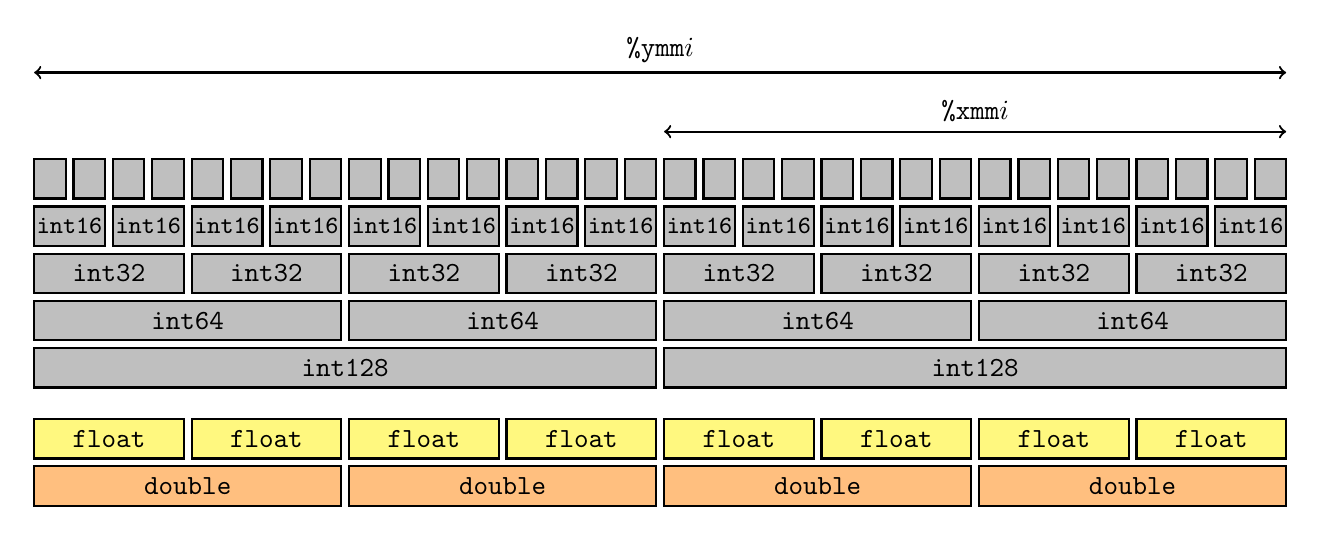
\begin{tikzpicture}[xscale=0.5, yscale=0.5]
  \foreach \i in {0, 8, 16, 24}
    \filldraw[thick, fill=orange, fill opacity=0.5] (\i, 0) rectangle +(7.8, 1);

  \foreach \i in {0, 4, ..., 31}
    \filldraw[thick, fill=yellow, fill opacity=0.5] (\i, 1.2) rectangle +(3.8, 1);

  \foreach \i in {0, 16}
    \filldraw[thick, fill=gray, fill opacity=0.5] (\i, 3) rectangle +(15.8, 1);

  \foreach \i in {0, 8, ..., 31}
    \filldraw[thick, fill=gray, fill opacity=0.5] (\i, 4.2) rectangle +(7.8, 1);

  \foreach \i in {0, 4, ..., 31}
    \filldraw[thick, fill=gray, fill opacity=0.5] (\i, 5.4) rectangle +(3.8, 1);

  \foreach \i in {0, 2, ...,  31}
    \filldraw[thick, fill=gray, fill opacity=0.5] (\i, 6.6) rectangle +(1.8, 1);

  \foreach \i in {0, 1, ...,  31}
    \filldraw[thick, fill=gray, fill opacity=0.5] (\i, 7.8) rectangle +(0.8, 1);

    \foreach \i in {0, 8, ..., 31}
    \path (\i, 0) rectangle node {\texttt{double}} +(7.8, 1);

    \foreach \i in {0, 4, ..., 31}
    \path (\i, 1.2) rectangle node {\texttt{float}} +(3.8, 1);

    \foreach \i in {0, 16}
    \path (\i, 3) rectangle node {\texttt{int128}} +(15.8, 1);

    \foreach \i in {0, 8, ..., 31}
    \path (\i, 4.2) rectangle node {\texttt{int64}} +(7.8, 1);

    \foreach \i in {0, 4, ..., 31}
    \path (\i, 5.4) rectangle node {\texttt{int32}} +(3.8, 1);

    \foreach \i in {0, 2, ..., 31}
    \path (\i, 6.6) rectangle node[font=\small] {\texttt{int16}} +(1.8, 1);

    \draw[thick,<->] (16, 9.5) -- node[above] {\texttt{\%xmm}$i$} +(15.8, 0);
    \draw[thick,<->] (0, 11) -- node[above] {\texttt{\%ymm}$i$} +(31.8, 0);
  \end{tikzpicture}
  \caption{Représentation des registres SIMD en SSE/AVX2.\label{fig:simd-reg}}
\end{figure}


\section{Écriture de programmes vectorisés}

problem with potential aliasing

\subsection{La vectorisation automatique}

\subsection{Directives OpenMP}

\subsection{Utilisation des fonctions \og intrinsèques\fg}


\section{Techniques générales}

Lorsqu'on cherche à \emph{paralléliser} un code, on cherche dans la mesure du
possible à découper le calcul en tâches plus ou moins indépendantes qu'on va
faire exécuter par plusieurs threads matériels simultanément. Le coût de la
création des tâches n'est pas négligeable, et donc il vaut mieux ne pas créer
trop de tâches. En présence d'un nid de boucles, la stratégie raisonnable
consiste généralement à paralléliser la boucle \emph{externe}.

\medskip

\begin{minipage}{0.55\textwidth}
\begin{minted}[fontsize=\small]{C}
/* Mauvais */
for (int i = 0; i < N; i++)
   for (int j = 0; j < N; j++) {
      double x = 0;
      #pragma omp parallel for reduction(+:x)
      for (int k = 0; k < N; k++)
         x += A[i * N + k] * B[k * N + j]
      C[i * N + j] = x;
   }
\end{minted}
\end{minipage}%
\begin{minipage}{0.45\textwidth}
\begin{minted}[fontsize=\small]{C}
/* Bon */
#pragma omp parallel for
for (int i = 0; i < N; i++)
   for (int j = 0; j < N; j++) {
      double x = 0;
      for (int k = 0; k < N; k++)
         x += A[i * N + k] * B[k * N + j]
      C[i * N + j] = x;
   }
\end{minted}
\end{minipage}

\medskip

Lorsqu'on cherche à \emph{vectoriser} un code, c'est l'inverse. La vectorisation
se déroule \emph{à l'intérieur} de chaque thread, et elle consiste à utiliser
les instructions SIMD lors du traitement de \og vecteurs\fg. Vu les contraintes
qui s'exercent (jeu d'instruction aux capacités limitées, etc.), la bonne
stratégie consiste généralement à vectoriser les portions de code les plus
courtes possibles, donc les boucles les plus \emph{internes}.

En plus, on peut combiner les deux : paralléliser les boucles externes (sur
plusieurs threads) tout en vectorisant les boucles internes (à l'intérieur d'un
seul thread).

Du coup, la vectorisation tourne principalement autour de l'étude de boucles
relativement simples. Lorsqu'il est possible d'obtenir que le code passe
l'essentiel de son temps dans la boucle à exécuter des instructions SIMD, on dit
que la boucle est vectorisée (ou vectorisable). Les boucles peuvent être
vectorisée quand il n'y a pas de dépendance entre itérations (\og
\anglais{loop-carried dependences}). Par exemple, il y a une dépendance de
données dans la boucle suivante :
\begin{minted}{C}
double u[];
...
for (int i = 1; i < n; i++)
    u[i] = u[i] + u[i-1];       // u[i] dépend de u[i-1];
\end{minted}
Les itérations de cette boucle ne peuvent pas être exécutées \og en parallèle\fg
par une instruction vectorielle ou SIMD.


\paragraph{Strip Mining}

La technique de base de la vectorisation est le \og \anglais{strip mining}\fg,
autrement dit le traitement par lot. Reprenons la petite boucle d'exemple qui
opère sur des vecteurs~:
\begin{minted}{C}
double u[];
...
for (int i = 0; i < n; i++)
    u[i] = u[i] + alpha * v[i];
\end{minted}

Supposons qu'on dispose des instructions AVX2, donc de registres SIMD capable de
contenir quatre \texttt{double}. La technique consiste grosso-modo à ré-écrire
la boucle de la façon suivante :
\begin{minted}{C}
double u[];
...
int m = n - (n % 4);
/* traitement par lots de 4 avec instructions SIMD */
for (i = 0; i != m; i += 4) {
    u[i + 0] = u[i + 0] + alpha * v[i + 0];
    u[i + 1] = u[i + 1] + alpha * v[i + 1];
    u[i + 2] = u[i + 2] + alpha * v[i + 2];
    u[i + 3] = u[i + 3] + alpha * v[i + 3];
}
/* épilogue au cas où n ne soit pas un multiple de 4 */
for (int i = m; i < n; i ++)
    u[i] = u[i] + alpha * v[i];
\end{minted}

\begin{danger}
  Le code assembleur obtenu ressemble à peu près à ceci. Noter la présence des
  instructions vectorielles \texttt{vmulpd} et \texttt{vaddpd}, signe que la
  vectorisation est effective.
  \begin{myfilet}
\begin{minted}{gas}
; %ymm2 = {alpha, alpha, alpha, alpha}, %rdx = adresse de v, %rsi = adresse de u 
.loop:
	vmulpd  (%rdx,%rax), %ymm2, %ymm1     ; %ymm1    <-- v[i:i+4] * %ymm2
	vaddpd  (%rsi,%rax), %ymm1, %ymm1     ; %ymm1    <-- %ymm1 + u[i:i+4]
	vmovapd %ymm1, (%rsi,%rax)            ; u[i:i+4] <-- %ymm1
	addq    $32, %rax                     ; i += 4 (32 octets)
	cmpq    %rcx, %rax                    ; compare i à m
	jne     .loop                         ; retourne en .loop si i != m
        ...
;       [si m == n, aller en .fin]
        ...
.epilogue:
	vmulsd  (%rdx,%rax), %xmm0, %xmm1     ; idem, mais en version scalaire
	vaddsd  (%rsi,%rax), %xmm1, %xmm1
	vmovsd  %xmm1, (%rsi,%rax,8)
	addq    $8, %rax                      ; i += 1 (8 octets)
	cmpl    %eax, %edi                    ; compare i à n
	jg      .epilogue                     ; recommence si i < n
.fin:
\end{minted}
  \end{myfilet}
\end{danger}

Du coup, la boucle de départ est transformée en \emph{deux} boucles : une qui
fait le gros du travail avec des instructions SIMD (\og \emph{kernel}\fg), et
une qui gère les éléments excédentaires (\og \emph{remainder}\fg).
\begin{danger}
  Parfois, il peut aussi y avoir un \emph{prologue} qui traite séquentiellement
  les premiers éléments pour obtenir un meilleur alignement. Les accès mémoire
  des instructions SIMD sont parfois plus efficaces lorsque les adresses sont
  bien alignées (sur un multiple de $x$ octets avec des vecteurs de $x$ octets).
  Certaines instructions spécifiques \emph{nécessitent} des adresses alignées,
  et déclenchent une erreur à l'exécution si ce n'est pas le cas.
\end{danger}

\paragraph{If Conversion}

L'adressage indirect (très présent dans le traitement des matrices creuses)
d'une part et la présence d'instructions conditionnelles d'autre part sont les
deux principaux obstacles à la vectorisation. Les instructions conditionnelles
sont particulièrement problématiques, car elles impliquent un traitement
différent selon les cases du vecteur. Ceci dit, on peut parfois les éliminer
(\og \emph{if conversion}\fg) en remplaçant la dépendance de contrôle par une
dépendance de données, par exemple en utilisant des \emph{masques}.

Voyons un exemple : la conversion entre espaces de couleur. Dans le monde du
graphisme (avec rendu sur écran), les couleurs sont généralement représentées en
rouge-vert-bleu (RGB --- on parle de synthèse additive ; plus on ajoute de
couleur plus ça devient blanc). Dans le monde de l'édition et de l'imprimerie,
les couleurs sont couramment représentées en cyan-magenta-jaune-noir (CMYK ---
on parle de synthèse soustractive ; plus on rajoute de couleur plus ça devient
noir). Pour simplifier, admettons que chaque composante est codée par un
flottant entre 0 et 1. La conversion entre les deux est donnée par:
\[
  \left\{
    \begin{array}{rl}
      R &= (1-C) \times (1 - K) \\
      G &= (1-M) \times (1 - K) \\
      B &= (1-Y) \times (1 - K)
    \end{array}
    \right.
\]
Cette conversion est facilement vectorisable : les trois vecteurs $(R, G, B)$
s'obtiennent à partir des quatre vecteurs $(C, M, Y, K)$ par addition et
multiplication coordonnée-par-coordonnée. Si on écrit :

\begin{minted}{C}
float R[__attribute__((aligned(64)));
for (int i = 0; i < n; i++)
\end{minted}


Dans l'autre sens, on a $K = 1 - \max(R, G, B)$ et le reste se déduit des
équations précédentes :
\[
  \left\{
    \begin{array}{rl}
      K &= 1 - \max(R, G, B) \\
      C &= 1 - R  / (1 - K) \\
      M &= 1 - G  / (1 - K) \\
      Y &= 1 - B  / (1 - K)
    \end{array}
    \right.
\]
Le problème, c'est que si on essaye de convertir la couleur noire ($R=G=B=0$) en
CMYK, l'application directe des formules provoque une division par zéro. La
division par zéro flottante n'interrompt pas l'exécution (elle renvoie un
flottant spécial représentant l'infini, ou bien \og not a number\fg), mais le
résultat sera faux quand même. Le programmeur consciencieux écrira donc :
\begin{minted}{C}
for (int i = 0; i < n; i++) {
    float max = R[i];
    if (G[i] > max)
        max = G[i];
    if (B[i] > max)
        max = B[i];
    K[i] = 1 - max;
    if (K[i] == 0.0) {
        C[i] = M[i] = Y[i] = 0.0;
    } else {
        C[i] = 1.0 - R / (1. - K);
        M[i] = 1.0 - G / (1. - K);
        Y[i] = 1.0 - B / (1. - K);
    }
}
\end{minted}

Or cette boucle n'est pas vectorisable telle quelle, à cause des instructions
conditionnelles. Les deux premières sont faciles à éliminer, car les unités SIMD
ont généralement une instruction min/max (\texttt{vmaxps} pour des vecteurs de 8
\texttt{float} en AVX). De toute façon, on pourrait calculer le max avec une
comparaison et des masques, comme décrit ci-dessous.

Le test sur la valeur de $K[i]$ nécessite l'emploi d'une technique générale : le
masquage. Les jeux d'instructions \og primitifs\fg (SSE, AVX, AVX2) incluent
généralement une instruction de comparaison qui produit un vecteur de
masques. Par exemple, l'instruction AVX \texttt{vcmpps} prend en argument deux
vecteurs de 8 \texttt{float} et renvoie un vecteur de 8 entiers 32 bits, qui
valent chacun \texttt{0xFFFFFFFF} ou \texttt{0x00000000} selon l'issue de la
comparaison entre les deux flottants correspondants. Grosso-modo, cela calcule
le vecteur $z$ défini par :
\begin{minted}{C}
z[i] = (x[i] < y[i]) ? 0xffffffff : 0x00000000;
\end{minted}
Ce vecteur de masques peut ensuite être utilisé avec des opérations booléennes
pour \og filtrer\fg des résultats. On peut donc utiliser la stratégie suivante :
faire systématiquement la division et ne garder le résultat que s'il a un sens.
Voici une implémentation possible, d'où les tests ont complètement disparu.

\begin{minted}{C}
for (int i = 0; i < n; i++) {
    // calcul du maximum avec des masques
    float max = R[i];
    int mask = (max < G[i]) ? 0xffffffff : 0x00000000;
    max = (G[i] & mask) | (max & ~mask);
    mask = (max < B[i]) ? 0xffffffff : 0x00000000;
    max = (B[i] & mask) | (max & ~mask);
    K[i] = 1 - max;
    // Valeur correcte si K != 0
    C[i] = 1.0 - R / (1. - K);
    M[i] = 1.0 - G / (1. - K);
    Y[i] = 1.0 - B / (1. - K);
    // Rattrapage éventuel. La valeur 0x00000000 est le flottant 0.0.
    mask = (K[i] > 0.0) ?  0xffffffff : 0x00000000;
    C[i] = C[i] & mask;
    M[i] = M[i] & mask;
    Y[i] = Y[i] & mask;
}
\end{minted}


% SIMD lane

% masques

% Today, the main factor that affects the success with which a program runs in
% vector mode is the structure of the program itself: Do the loops have true data
% dependences (see Section 4.5), or can they be restructured so as not to have such
% dependences? This factor is influenced by the algorithms chosen and, to some
% extent, by how they are coded.


% The elements of a vector in storage may be contiguous, or
% they may be separated by one or more element positions. The
% number of element positions by which a vector operation
% advances to progress from one element to the next is the vector
% stride. Important cases are stride 1, where the vector elements
% are in contiguous locations, and stride 2, which appears in
% complex-number calculations. Stride N refers to a general
% stride other than 1 or 2.

\paragraph{Opérations \og horizontales\fg}

Parfois, on a besoin de faire interagir entre elles les composantes d'un même
vecteur. On parle alors d'opération \og horizontale\fg. Par exemple, pour
calculer la norme d'un vecteur, on a besoin de calculer la somme des carrés de
ses composantes.

\begin{minted}{C}
double u[];
double n = 0;
...
for (int i = 0; i < n; i++)
    n = n + u[i] * u[i];
\end{minted}
A première vue, il y a une dépendance de données sur $n$ ; chaque itération lit
le résultat de l'itération précédente. Mais en fait, on peut s'en tirer avec une
\emph{réduction}.

\begin{minted}{C}
double n[4] = {0, 0, 0, 0};
int m = n - (n % 4);
/* traitement par lots de 4 avec instructions SIMD */
for (i = 0; i != m; i += 4) {
    n[0] = n[0] + u[i + 0] * u[i + 0];
    n[1] = n[1] + u[i + 1] * u[i + 1];
    n[2] = n[2] + u[i + 2] * u[i + 2];
    n[3] = n[3] + u[i + 3] * u[i + 3];
}
/* épilogue au cas où n ne soit pas un multiple de 4 */
for (int i = m; i < n; i ++)
    n[0] = n[0] + u[i] * u[i];
/* réduction */
double n = n[0] + n[1] + n[2] + n[3];
\end{minted}

truc super malin dans le papier ARM SVE sur arXiv pour suivre une liste chaînée (loop fission) :
\begin{minted}{C}
struct{uint64 val; struct node* next} *p;
uint64 res = 0;
for(p = &head; p != NULL; p = p->next)
    res ˆ= p->val;
///// séparer la partie séquentielle de la partie vectorisable.
for(p = &head; p != NULL; ) {
    for(i = 0; p != NULL && i < VL/64; p = p->next)
p'[i++] = p; // collect up to VL/64 pointers
for(j = 0; j < i; j++)
    res ˆ= p'[j]->val; // gather from pointer vector
\end{minted}




\section{Vecteurs de longueur inconnue}

\epigraph{If You Think Education Is Expensive, Try Ignorance}{Robert Orben}





\part{Aspects théoriques}

\chapter{Bornes inférieures}

Modèle VLSI. Intérêt du produit $AT$ pour maximiser le débit. $AT$ est une
mesure d'énergie; $AT^2$ est une mesure de puissance.

Raisonnements asymptotiques; ne parle pas du nombre de multiplicateurs flottants
64 bits qu'on peut mettre sur un CPU.

\section{Nécessité de mémoriser des données}

Un raisonnement assez simple permet de montrer que dans un certain nombre de
cas, n'importe quel circuit qui implémente une fonction donnée doit être assez
\emph{gros}, c'est-à-dire occuper une certaine surface.

L'idée générale consiste à dire que le circuit ne peut pas produire le résultat
au fur-et-à-mesure qu'il lit son entrée. Il doit d'abord lire une partie de
l'entrée sur ses ports d'entrée \emph{avant} de commencer à envoyer le résultat
sur ses ports de sortie. Ceci implique qu'il \emph{mémorise} une partie de
l'entrée, or la mémoire occupe de la surface.

C'est le cas des circuits suivants :
\begin{itemize}
\item Rotation: un circuit qui prend en argument une chaine de bits
  $x \in \bits^N$ ainsi qu'un entier $0 \leq k < n$ et renvoie $x^{\lll k}$ doit
  avoir une surface $A = \bigOmega{N}$ (Si $abcd \in \{0, 1\}^4$, alors
  $abcd^{\lll 1} = bcda$, $abcd^{\lll 2} = cdab$, etc.)

\item Multiplication : un circuit qui prend en argument deux entiers de $N$ bits
  et qui renvoie leur produit sur $2N$ bits doit avoir une surface
  $A = \bigOmega{N}$.

\item Tri: Un circuit qui trie $N$ nombres de $k$ bits (avec
  $k \geq 2 \log_2 N$) possède une aire $A = \bigOmega{N}$.

\item Produit de matrice : un circuit qui multiplie deux matrices (de bits ou
  d'entiers de $k$ bits) de taille $n \times n$ doit avoir une surface $A = \bigOmega{n^2}$.

\item Transformée de Fourier, produit de polynômes, etc. $\to$ surface $A = \bigOmega{n}$.
\end{itemize}

\begin{danger}
  Le cas de la rotation est le plus simple à comprendre : supposons que le
  circuit possède $p_{in}$ ports d'entrée et $p_{out}$ ports de sortie. Si
  $p_{in} = N$ ou $p_{out} = N$, alors le circuit est de surface supérieure à
  $N$ et le résultat est établi. Sinon, le circuit lit son entrée en plusieurs
  temps (il faut au moins $N / p_in$ cycles; il lit les bits de $x$ dans un
  ordre quelconque, toujours le même) et produit sa sortie en plusieurs temps
  (il faut au moins $N / p_{out}$ cycles ; il produit les bits de $z$ dans un
  ordre quelconque). Notons $b$ un bit de $x$ qui entre dans le circuit lors du
  dernier cycle de lecture. On peut choisir une valeur de $k$ tel que ce bit
  apparaît dans le premier cycle d'écriture du résultat. Par conséquent, le
  résultat ne peut pas être produit tant que l'entrée n'a pas été entirèrement
  lue. Ceci signifie que le circuit est capable de mémoriser $N$ bits, donc
  qu'il a une surface d'au moins $N$. Ceci est démontré dans~\cite{Vuillemin83}.

  Pour la multiplication, c'est nettement moins
  direct. Cf.~\cite{BrentK80}. Mais si on considère la fonction
  $(a, b, M) \mapsto ab \bmod M$, alors c'est facile : avec $M = 2^n - 1$,
  multiplier par $2^k$ revient à faire une rotation de $k$ bits et permet de se
  ramener au résultat précédent.

  Le tri permet de réaliser une permutation arbitraire d'une chaine de bits
  $x \in \bits^N$, et en particulier la rotation. La taille des entiers à trier
  permet qu'ils soient tous différents même si on \og gomme\fg leur bit de poids
  faible. Choisissons une permutation $\sigma$ des $\log_2 N$ bits de poids
  forts, et trions la liste $[2 \sigma(1) + x_1; \dots; 2 \sigma(n) + x_n]$. Le
  résultat est
  $[ 2 + x_{\sigma^ {-1}(1)}; 4 + x_{\sigma^ {-1}(2)} ; 6 + x_{\sigma^ {-1}(3)};
  \dots ]$. Le circuit lit et écrit ses bits dans un ordre arbitraire;
  choisissons la permutation $\sigma$ de telle sorte que le dernier $x_i$ lu est
  le premier écrit : le circuit doit mémoriser $N$ bits.

  Pour le produit de matrice, l'argument consiste à dire que l'une des deux
  matrices peut être une matrice de permutation, donc que n'importe quelle
  ligne/colonne de l'autre peut être émis en premier, ce qui nécessite de les
  mémoriser toutes. Cf~\cite{ChazelleM81}.
\end{danger}


\section{Espace occupé par les fils}

Contrairement au modèle de calcul usuel (la machine RAM) qui est assez évasif
sur la réalisation physique du calcul, dans le monde matériel, transmettre des
informations a un coût, et ce coût peut dominer celui des \og calculs\fg à
proprement parler.

Au début des années 1980, des bornes inférieures sur la complexité matérielle de
nombreuses fonctions ont pu être démontrées. Ces bornes fonctionnent grosso-modo
de la façon suivante (cf.~\cite{Thompson79}).

\begin{itemize}  
\item Imaginons qu'on coupe le circuit en deux, avec environ autant de ports
  d'entrée dans les deux moitiés. Ceci coupe $w$ fils. Un petit raisonnement
  géométrique permet de se convaincre que ces fils doivent occuper une surface
  $A = \bigOmega{w^2}$.

\item En raisonnant sur la fonction calculée par le circuit, on parvient à
  établir que la réalisation du calcul nécessite qu'une certaine quantité
  d'information (typiquement $\bigOmega{n}$ bits où $n$ est la taille de
  l'entrée) soit transmise sur ces fils. Or ceci nécessite $\bigOmega{n/w}$
  unités de temps.

\item En combinant les deux, on trouve $AT^2 = \bigOmega{n^2}$.
\end{itemize}

\medskip

Des bornes de ce type en $AT^2 = \bigOmega{n^2}$ ont été démontrées pour le
calcul de la transformée de Fourier~\cite{Thompson79}, la multiplication des
entiers~\cite{BrentK80}, le tri, la multiplication des matrices~\cite{Savage81},
etc. etc. etc. Généralement, des circuits qui atteignent ces bornes sont
connus.

En outre, comme on sait que la taille de ces circuits est généralement en
$A = \bigOmega{n}$, on peut en déduire que $T = \bigOmega{\sqrt{n}}$. Par
conséquent, on en déduit que dans ces cas-là $AT = \bigOmega{n^{1.5}}$.

Ceci démontre par exemple que le \anglais{mesh} de taille $n \times n$ qui trie
$n^2$ entiers en temps $n$ est optimal.

Il y a une exception notable : l'addition de deux entiers de $n$ bits. On a
alors $AT / log A = \bigOmega{n}$. Il existe un circuit additionneur avec $A=1$
et $T=\bigO{n}$ d'une part, et un autre avec $A = \bigO{n \log n}$ et
$T = \bigO{log n}$ d'autre part.

Tous ces résultats reposent de manière crucial sur le caractère \emph{plat} des
circuits considérés. Ceci dit, rien ne s'oppose à une généralisation en 3
dimensions. Par exemple (cf.~\cite{Wiener04}), supposons que $p$ processeurs
aient accès à une mémoire partagée taille $m$. Si chaque processeur accède à une
adresse aléatoire de la mémoire toutes les $1/f$ unités de temps ($f$ est une
fréquence), alors la longueur totale des fils qui relient les processeurs à la
mémoire est minorée par $\bigOmega{(pf)^{3/2}}$.

Les fils peuvent donc occuper plus de place que les processeurs ou la mémoire,
si $f$ est trop élevé. Par exemple si $f = 1$ (les processeurs accèdent à la
mémoire à chaque cycle), alors les fils sont de longueur au moins $p \sqrt{p}$.

\section{Vitesse de la lumière}

Les résultats de la section précédente sont de nature combinatoire ou
géométrique : aucune hypothèse n'est faite sur les \emph{délais de propagation}
de l'information d'un point $A$ à un point $B$. Les bornes sur $T$ supposent que
l'information se déplace instantanément.

Or, ceci est manifestement faux sur de grandes distances. Si on suppose que
l'information met un temps $\bigO{d}$ pour parcourir une distance $d$. Du coup,
la longueur des fils a une influence sur le temps de calcul. Il se trouve que
ceci interdit complètement les calculs en temps logarithmique
(cf.~\cite{ChazelleM81}), et impose des bornes inférieurs en $\sqrt{n}$ dans
bien des cas.

\begin{danger}
Un argument assez simple permet de le démontrer pour le tri : comme tous les
bits de la sortie dépendent de tous les bits de l'entrée, il faut que les ports
d'entrée et de sortie se trouve à l'intérieur d'un cercle de rayon $\bigO{T}$,
sinon l'information n'a pas le temps de voyager de l'entrée à la sortie. De
plus, tous les composants qui contribuent à la valeur sur un port de sortie
doivent se trouver à distance inférieure à $\bigO{T}$ de ce port de sortie-là.

Par conséquent, la surface totale des composants qui participent au calcul est
limitée par $A = \bigO{T^2}$. Comme on a vu que $A = \bigOmega{n}$ et
$AT^2 = \bigOmega{n^2}$, on trouve fatalement que $T = \bigOmega{\sqrt{n}}$.
\end{danger}

En particulier, pour l'addition, ceci implique que $T = \bigOmega{\sqrt{N}}$ et
$AT = \bigOmega{N}$.

\begin{danger}
  En effet, considérons un circuit qui calcule la fonction booléenne qui calcule
  le bit de poids fort du résultat. Ce dernier dépend de tous les bits
  d'entrée.
  % L'ensemble des composants qui
  % participent au calul doivent se trouver à l'intérieur d'un cercle de rayon
  % $\bigO{T^2}$ autour du point où le résultat est obtenu : s'ils sont plus
  % loin,
  % alors ils n'ont pas le temps de communiquer avec la partie du circuit qui
  % renvoie le résultat. Les $n$ bits d'entrées sont délivrés par $p$ portes
  % logiques, avec $p \leq n$. La lecture des entrées prend un temps au moins
  % $n/p$.

  % $A \geq p$, donc $T \geq \sqrt{p}$.
  les données doivent être lues depuis $p$ ports, ce qui prend un temps
  $N/p$. Les ports sont à la périphérie d'un polygone convexe de périmètre au
  moins $p$, donc le points de rassemblement est à distance $\bigOmega{p}$ de
  l'un d'entre eux. Les données vont donc mettre un temps $\bigOmega{p}$ pour
  voyager du port d'entrée le plus éloigné jusqu'au point de rassemblement. Cela
  donne un temps total $\bigOmega{N/p + p}$. Ceci est plus grand que $\sqrt{N}$
  (minimum atteint lorsque $p = \sqrt{N}$).
\end{danger}


\chapter{Synchronisation et modèles mémoires relâchés}

\section{Modèle mémoire de \OMP}

Tant qu'on se tient à la règle de base de la programmation avec \OMP
(utiliser \texttt{atomic} + \texttt{critical} pour tous les accès
potentiellement
conflictuels), % la \anglais{sequential consistency} est garantie et
on ne devrait pas avoir de problème.

Ceci dit, si on veut aller plus loin, par exemple parce qu'on a des problème de
performance liés au coût des synchronisations, il faut être conscient qu'\OMP
n'offre que des garanties assez faibles sur ce qui se passe lors des
\emph{autres} accès à la mémoire partagée.

Ces garanties sont formalisées dans le \emph{modèle mémoire} offert
par \OMP. Ce modèle mémoire est dit \og relâché\fg ou \og faible\fg{}
(\anglais{relaxed}, \anglais{weak}) car il ne garantit pas que les
différents threads aient une vue cohérente du contenu de la mémoire
partagée. En particulier, il ne garantit \emph{pas du tout} que des
threads soient correctement synchronisés par des accès mémoires % la
% \anglais{sequential consistency} pour les accès mémoire
non-protégés
par \texttt{atomic} ou \texttt{critical}.

\subsection{Description}

\begin{itemize}
\item Tous les threads ont accès à la mémoire partagée.

\item Cependant, chaque thread peut avoir une \emph{vue temporaire privée} de la
  mémoire. La nature précise de cette vue temporaire privée ne fait pas partie
  de la description de \OMP, mais peut être matérialisée par des données
  stockées dans des registres du processeurs, dans des caches, etc.

\item La vue temporaire de la mémoire d'un thread n'est pas nécessairement
  synchronisée en permanence avec le contenu de la mémoire partagée.

\item Une valeur écrite dans une variable par un thread peut rester dans sa vue
  temporaire pendant un certain temps, jusqu'à ce qu'elle soit finalement \og
  poussée\fg vers la mémoire. Du coup, la modification n'est pas forcément
  visible instantanément par les autres threads.

\item Une valeur lue depuis une variable partagée peut provenir de la vue
  temporaire du thread et être \og périmée\fg (une valeur plus récente a été
  écrite en mémoire, mais la vue temporaire du thread n'a pas été rafraîchie.

\item La vue temporaire d'un thread peut être \emph{synchronisée} avec
  la mémoire partagée, c'est-à-dire que si le contenu de la mémoire
  partagée a changé, la vue temporaire privée est mise à jour, et si
  des variables ont changé dans la vue temporaire privée, la mémoire
  partagée est mise à jour.
  
\item Les vue temporaires privées des threads sont synchronisées avec
  la mémoire partagée à certains moments : lors de \texttt{omp
    barrier} ; lors de la sortie de toutes les constructions de
  partage de travail (\texttt{omp for}, \texttt{omp sections} et
  \texttt{omp single}) ; lors de l'entrée et de la sortie de
  \texttt{omp parallel}, \texttt{omp critical}, \texttt{omp atomic} ;
  lors de chaque point d'ordonnancement/annulation des tâches. Dans
  cette liste, les exceptions notables sont l'entrée des constructions
  de partage de travail ainsi que l'entrée et la sortie de \texttt{omp
    master}.

\item On peut forcer la synchronisation avec \texttt{omp flush} (en \og mode gourou\fg uniquement).
\end{itemize}

\medskip

On pourrait faire une analogie avec les systèmes de contrôle de
version tels que \marque{git} avec lesquels les programmeurs sont
familiers : chaque développeur possède sa \og copie privée\fg du code
et se synchronise avec une copie centrale de temps en temps.

Ceci est similaire au modèle PRAM~\cite{Lipton1988PramAS} décrit à la fin des
années 1980. Chaque processeur possède une mémoire locale. Les processeurs
effectuent les lectures depuis leurs mémoires locales. Pour effectuer une
écriture, un processeur écrit dans sa mémoire locale, puis envoie un
\emph{message} à chacun des autres processeurs pour les informer de
l'écriture. Aucune confirmation n'est attendue et l'exécution continue. Les
accès à la mémoire sont donc des opérations \emph{locales} qui n'induisent pas
de synchronisation. Quand un message arrive sur un processeur, il est
automatiquement exécuté (la mémoire locale est mise à jour). Mais les temps de
transport sur le réseau sont très variables... et les messages peuvent même se
doubler ! Ceci est illustré par la figure~\ref{fig:pram}.

\begin{figure}
  \centering
  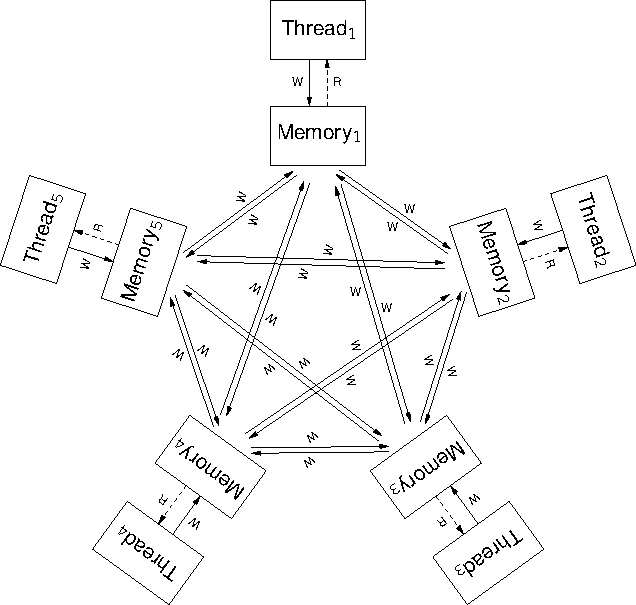
\includegraphics[width=0.75\textwidth]{pram_archi}
  \caption{Représentation du modèle PRAM / \OMP. Chaque processeur possède
    une \og copie locale\fg de la mémoire, et se synchronise avec les
    autres par transfert de messages (image~:~A Tutorial Introduction
    to the ARM and POWER Relaxed Memory Models). \label{fig:pram}}
\end{figure}

%Meunier : 
% Les écritures effectuées par un même processeur sont vues par les
% autres processeurs dans l’ordre dans lequel elles ont été effectuées,
% mais les écritures venant de processeurs différents peuvent être vues
% dans des ordres différents par différents processeurs


\subsection{Comportements relâchés autorisés par le modèle mémoire \OMP}
\label{sec:relaxed-behaviors}

Ce modèle mémoire est dit \og relâché\fg{} car il autorise les
comportements suivants qui dévient de l'intuition des programmeurs :
\begin{itemize}
\item Un thread écrit dans une variable et les autres threads ne
  perçoivent pas l'écriture tout de suite.
  
\item Un thread écrit dans deux variables alors qu'un autre
  thread perçoit seulement la première écriture et pas la deuxième.

\item Un thread écrit dans deux variables alors qu'un autre
  thread perçoit seulement la deuxième écriture et pas la première.

\item Un premier thread écrit dans deux variables alors qu'un
  deuxième thread perçoit seulement la première écriture tandis qu'un
  troisième thread perçoit seulement la deuxième.
\end{itemize}

\medskip

En l'absence de précautions particulières, tout ceci fait échouer des
mécanismes pourtant intuitifs de synchronisation entre les threads.

\paragraph{Exclusion mutuelle du pauvre} Considérons un mécanisme
d'exclusion mutuelle particulièrement simple entre deux threads. Si un
des threads veut entrer dans la section critique (c.a.d. acquérir le
verrou), il met à 1 son \texttt{flag} puis attend que le \texttt{flag}
de l'autre soit à zéro.

\begin{myfilet}
\begin{minted}{C}
bool flag[2];

void lock() 
{
	int i = omp_get_thread_num();
	flag[i] = true;                    // I'm interested
	while (flag[1 - i]) {};            // wait if the other is also interested
}

void unlock() 
{
	int i = omp_get_thread_num();
	flag[i] = false;                   // I'm no longer interested
}
\end{minted}
\end{myfilet}

Ce mécanisme semble pouvoir garantir l'exclusion mutuelle : si jamais
les deux threads parvenaient à appeler \texttt{lock()} puis à entrer
dans la section critique en même temps, alors \mintinline{C}{flag[0] == flag[1] == true}.
Mais ceci semble impossible à cause des boucles
\texttt{while} qui protègent l'accès à la section critique.

\begin{danger}
  Cet algorithme a un gros problème : si les deux threads appellent
  \texttt{lock()} en même temps, alors ils vont se retrouver bloqués
  tous les deux (ils sont en \anglais{deadlock}). Le \emph{Peterson
    lock} dont il est question section~\ref{sec:peterson-proof} est
  bien meilleur et n'a pas ce problème.
\end{danger}

En réalité, dans le modèle mémoire \OMP, ceci peut échouer complètement :
\begin{itemize}
\item Les deux threads écrivent \mintinline{C}{flag[i] = true} dans leur vue temporaire privée de la mémoire partagée.
\item Ils lisent \mintinline{C}{flag[1 - i] == false} depuis leur vue temporaire privée.
\item Ils entrent tous les deux dans la section critique.
\end{itemize}
\medskip

Le problème vient du fait que leurs vue privées temporaires ne sont pas
forcément synchronisées entre elles.

\paragraph{Passage de message} Considérons un problème de \og
producteur-consommateur\fg{} particulièrement simple, à deux threads :
le premier thread va produire des données tandis que le deuxième
attend que les données soient prêtes pour les utiliser. Le premier
appelle \texttt{produce()} avec l'adresse des données prêtes. Le
deuxième appelle \texttt{consume()} pour attendre et récupérer
l'adresse des données.

\begin{myfilet}
\begin{minted}{C}
bool ready = false;
void * data = NULL;

void * consume() 
{
	while (ready == false) {};     // wait
        return data; 
}

void produce(void * payload) 
{
        data = payload;
        ready = true;
}
\end{minted}
\end{myfilet}

Ceci peut complètement échouer dans le modèle mémoire \OMP. Plus
précisément, après un appel de \texttt{produce(x)}, \texttt{consume()}
pourrait renvoyer un pointeur nul (au lieu de \texttt{x}). La séquence
d'évènement problématique est la suivante ($P$ désigne le thread
producteur et $C$ le thread consommateur)~:
\begin{itemize}
\item $P$ écrit \texttt{data} dans sa vue temporaire privée.
\item $P$ écrit \texttt{ready} dans sa vue temporaire privée.
\item L'écriture \texttt{ready} est propagée de la vue temporaire privée de $P$ à la mémoire partagée.
\item L'écriture \texttt{ready} est propagée de la la mémoire partagée à la vue temporaire privée de $C$.
\item $C$ lit \texttt{ready == true} et se débloque.
\item $C$ lit \texttt{data == NULL} depuis sa vue temporaire privée.
\end{itemize}


\subsection{Justification de la \og faiblesse\fg du modèle mémoire}

Le modèle mémoire \OMP casse un certain nombre d'intuition que les programmeurs
habitués aux machines séquentielles peuvent avoir sur le fonctionnement de la
mémoire. Mais il est dans le fond adapté pour des raisons de performance et
d'architecture matérielle. En effet, les compilateurs d'une part et le matériel
d'autre part se permettent un certain nombre de libertés dans la façon dont le
code écrit par les programmeurs est traduit et exécuté. Ces libertés ne sont pas
perceptibles dans la programmation séquentielle, mais elles le devienent en
multi-threads. Le modèle mémoire \OMP incorpore ces libertés.

\paragraph{Les compilateurs} Les compilateurs, surtout lorsqu'ils tentent
d'optimiser le code produit, gardent au maximum les valeurs des variables dans
les registres du processeur. Ceci constitue alors une \og vue temporaire
privée\fg : pendant que la valeur d'une variable $x$ est stocké dans le registre
\texttt{\%rax} du CPU, elle n'est pas \og synchronisée\fg avec sa valeur en
mémoire.

Ceci est illustré par le petit bout de code suivant. Le thread $T_0$ fait
$2 \cdot 10^6$ iterations tandis que $T_1$ n'en fait que la moitié, et va donc
sortir de la boucle en premier, puis modifier $n$. Mais ceci ne sera pas perçu
par $T_0$ qui reste avec sa \og vue privée temporaire\fg. Quand $T_0$ sort de sa
section parallèle, sa vue privée temporaire est synchronisée avec la mémoire
partagée, donc il écrit \emph{sa} valeur de $n$ en mémoire.

\begin{myfilet}
\begin{minted}{C}
double n = 0, m = 0xDEADBEEF;
#pragma omp parallel num_threads(2)
{
	int i = omp_get_thread_num();
	for (int j = 0; j < 1000000 * (1 + (i == 0)); j++) {
		if (i == 0)
			n += 1.0;
		else
			m += 1.0;
	}
	if (i == 1)
		n = m;
}
printf("n = %.0f, m = %.0f\n", n, m);
\end{minted}
\end{myfilet}

On obtient :
\begin{verbatim}
n = 2000000, m = 3736928559
\end{verbatim}

\begin{danger}
  Un petit examen du code assembleur produit par le compilateur confirme
  ceci. On voit clairement que $n$ et $m$ sont copiées dans des registres au
  début de la boucle, puis restaurées en mémoire à la fin de la boucle.
\begin{myfilet}
\begin{minted}{asm}
parallel_section:
	pushq   %rbx                       ; préambule
	movq    %rdi, %rbx                 ;
	call    omp_get_thread_num@PLT     ; i = omp_get_thread_num()
	movsd   8(%rbx), %xmm0             ; lire la valeur de m en mémoire, stocker dans %xmm0
	movsd   (%rbx), %xmm1              ; lire la valeur de n en mémoire, stocker dans %xmm1
	testl   %eax, %eax                 ; if (i == 0) ...
	je      T_0                        ;    ... goto T_0
T_1:
	movsd   .LC0(%rip), %xmm2          ; %xmm2 = 1.0
	movl    $1000000, %edx             ; j = 1000000
loop1:
	addsd   %xmm2, %xmm0               ; m += 1.0
	subl    $1, %edx                   ; j--
	jne     .L3                        ; if (j != 0) goto loop1
	movsd   %xmm0, 8(%rbx)             ; écrire la valeur de m en mémoire depuis %xmm0
	cmpl    $1, %eax                   ; if (i == 0) ...
	jne     .L1                        ;    ... goto end1
	movsd   %xmm0, (%rbx)              ; écrire la valeur de n en mémoire depuis %xmm1
end1:
	popq    %rbx                       ; fin de la section parallèle
	ret

T_0:
	movsd   .LC0(%rip), %xmm2          ; %xmm2 = 1.0
	movl    $2000000, %eax             ; j = 2000000
loop0:
	addsd   %xmm2, %xmm1               ; n += 1.0;
	subl    $1, %eax                   ; j--
	jne     loop0                      ; if (j != 0) goto loop1
	movsd   %xmm1, (%rbx)              ; écrire la valeur de n en mémoire depuis %xmm1
	popq    %rbx                       ; fin de la section parallèle
	ret
\end{minted}
\end{myfilet}
\end{danger}%$

\paragraph{Le matériel} Il y en outre des raisons architecturales. Presque
toutes les architectures matérielles des microprocesseurs actuels\footnote{en
  tout cas ceux de la famille RISC : les \marque{ARM}, \marque{POWER},
  \marque{SPARC}, \marque{MIPS}, \marque{RISC-V}, etc. et même les
  \marque{x86-64} si on gratte un peu sous le jeu d'instruction qui date de la
  fin des années 1970...} sont de type \anglais{load-store} : les opérations
arithmétiques ne peuvent se faire qu'entre les registres du processeur, et pas
de/vers la mémoire. Il faut donc, dans l'ordre : 1) charger les données dans des
registres (\anglais{load}) ; 2) faire les calculs; 3) écrire le résultat en
mémoire (\anglais{store}). Sur un tel processeur, le thread a une \og vue temporaire privée\fg{}
du contenu de la mémoire à partir de la fin de l'étape 1 (la valeur est chargée
dans un registre ; même si elle change en mémoire pendant l'étape 2 ou 3,
l'ancienne valeur reste dans le registre du processeur). On verra de plus section~\ref{sec:CPU-not-SC}
que les processeurs exhibent parfois naturellement les comportement relâchés décrits plus hauts (section~\ref{sec:relaxed-behaviors})

Voyons un autre exemple\footnote{DISCLAIMER : Le programme de test
  n'est pas aussi simple que voulu. Je voulais initialement faire ce test avec
  \mintinline{C}{for (int i = 0; i < 1000000000; i++) x++;}, mais le compilateur
  \marque{gcc 8.3.0} est suffisamment évolué pour remplacer automatiquement ceci
  par \mintinline{C}{x = 1000000000;}...}~:
\begin{myfilet}
\begin{minted}{C}
int x[2] = {};
#pragma omp parallel for
for (int i = 0; i < 1000000000; i++) {
        int j = i & 0x00000001;  /* récupère le bit de poids faible de i */
	x[j]++;	
}
for (int i = 0; i < 2; i++)
        printf("x[%2d] : %10u\n", i, x[i]);
\end{minted}
\end{myfilet}

Comme il y a autant d'entiers pairs et impairs dans l'intervalle $[0; 10^9[$, on
s'attend à voir apparaître la valeur $5 \cdot 10^8$ dans les deux cases de
\texttt{x}. C'est bien le cas si on exécute ce code en désactivant \OMP lors de
la compilation. Résultat avec \OMP (sur un laptop à deux coeurs x86-64) :
\begin{verbatim}
        x[ 0] :  262301234
        x[ 1] :  262261007
\end{verbatim}

Le programme ne produit \emph{jamais} les bonnes valeurs. Le problème, c'est que
l'instruction \texttt{x[j]++;} du langage \marque{C} n'est pas
\emph{atomique}. Au contraire, elle se décompose en trois phases :
\begin{enumerate}
\item Charger $x[j]$ depuis la mémoire vers le CPU.
\item Incrémenter la valeur.
\item Écrire le résultat dans la mémoire.
\end{enumerate}

Voici (vraissemblablement) ce qui se passe lors de l'exécution du test~:
\begin{enumerate}  
\item Le thread 0 lit la valeur de $x[j]$.
\item Le thread 1 lit la valeur de $x[j]$ (c'est la même).
\item Le thread 0 écrit dans $x[j]$ une nouvelle valeur.
\item Le thread 1 écrit dans $x[j]$ une nouvelle valeur, et écrase la valeur écrite à l'étape précédente.
\end{enumerate}

Ceci explique qu'on voit apparaître des valeurs plus faibles que
celles attendues (puisque l'écriture du deuxième threads \og écrase\fg
l'incrémentation effectuée par le premier). Ce problème doit être
contourné par des moyens logiciels, car sur les architectures
\anglais{load-store}, la procédure en trois étapes décrite ci-dessus
est inévitable.

\begin{danger}
%\begin{minipage}[*]{\textwidth}
  \footnotesize
  Un examen du code assembleur généré par \marque{gcc} sur un
  \marque{Raspberry Pi}, donc un \marque{ARM}, le confirme. On voit bien
  apparaître la séquence \texttt{ldr} (\anglais{LoaD into Register}) \texttt{;
    add; str} (\anglais{STore from Register}).
\begin{myfilet}
\begin{minted}{asm}
; r0 contient 10^9
; r2 contient i
; r3 contient j
; x se trouve à l'adresse sp
; r1 contient l'adresse de x[j]
loop:
	and	r3, r2, #1          ; j = i & 0x00000001
	add	r1, sp, #8          ; [calcul de l'adresse de x[j]
	add	r3, r1, r3, lsl #2  ; r3 = adresse de x[j]
	add	r2, r2, #1          ; i++
	ldr	r1, [r3, #-8]       ; tmp = x[j]
	cmp	r2, r0              ; si i < 10^9...
	add	r1, r1, #1          ; tmp = tmp + tmp + 1
	str	r1, [r3, #-8]       ; x[j] = tmp
	bne	loop                ; ... alors goto loop
\end{minted}
\end{myfilet}
\end{danger}

De toute façon, même sur les processeurs qui ne sont pas explicitement conçus
sur l'architecture \anglais{load-store}, comme les \marque{x86-64}, le problème
a lieu aussi (et d'ailleurs le test le démontre).

\begin{ddanger} La situation est même encore pire, car le test démontre en fait
  que l'exécution d'instructions \emph{individuelles} du processeur n'est même
  pas atomique. En effet, \emph{une seule} instruction permet d'incrémenter
  l'entier situé en mémoire à l'adresse donnée (donc, en théorie pas de besoin
  de \texttt{load/add/store}. Le compilateur \marque{gcc} l'utilise dans le
  test, et il génère le code assembleur suivant~:

  \begin{myfilet}
\begin{minted}{asm}
; %edx contient i
; le tableau x est à l'adresse %rsi
; %ecx contient j
; %ecx contient tmp
; %eax contient la borne de la boucle
loop:
	movl	%edx, %ecx            
	addl	$1, %edx              ; i++
	andl	$1, %ecx              ; j = i & 0x00000001
	addl	$1, (%rsi,%rcx,4)     ; x[j]++        (x[j] est à l'adresse %rsi + 4 * %rcx)
	cmpl	%edx, %eax            ; si i < 10^9...
	jne	loop                  ; ... alors goto loop
\end{minted}
  \end{myfilet}
  L'instruction \texttt{addl} ajoute son premier opérande au deuxième,
  c'est-à-dire pour celle qui nous intéresse la constante 1 au contenu de la
  case mémoire \verb|(%rsi,%rcx,4)| qui contient
  $x[j]$. Eh bien ce que le test montre, c'est que cette instruction \emph{ne
    s'exécute pas de manière atomique}.
\end{ddanger}%$

\section{La \og \anglais{Sequential Consistency}\fg}

\subsection{La \og \anglais{strict consistency}\fg}

Lorsqu'on a l'habitude d'écrire des programmes qui s'exécutent séquentiellement,
sur une machine de type \og architecture de Von Neumann\fg, on développe un
modèle mental dans lequel la mémoire nous offre une garantie très forte :
\important{toute lecture d'une variable renvoie la dernière valeur écrite
  dedans}. Nous avons aussi l'habitude que les systèmes de fichiers offrent à
peu près cette garantie.

Cette garantie s'appelle la \og \anglais{strict consistency}\fg. Les compilateurs et les
processeurs garantissent que ce modèle est respecté par les programmes
séquentiels, et la notion a du sens : dans un programme séquentiel, on
peut parler de \emph{la} dernière valeur écrite dans une variable.

\begin{danger}
  En réalité, compilateurs et processeurs prennent des libertés
  importantes avec la \anglais{strict consistency}, mais ils se débrouillent
  pour que ça n'affecte pas la sémantique des programmes séquentiels, et la
  plupart des programmeurs n'en ont pas conscience. Mais ça peut affecter les
  programmes parallèles ! Plus de détails ci-dessous.
\end{danger}

Sur des machines parallèles, les choses deviennent plus compliquées. Pour
commencer, sur une machine à plusieurs coeurs, que se passe-t-il si plusieurs
\emph{threads} décident d'écrire des valeurs différentes à la même adresse
mémoire \emph{en même temps} ?

\paragraph{En parallèle, la \anglais{strict consistency} n'a pas de sens} Le
problème dans les machines parallèles, c'est qu'il n'y a pas de notion
raisonnable d'un \emph{temps global}.

Premier exemple : imaginons une variable $x$ stockée sur une machine $S$ (comme
Serveur). Dans le \anglais{rack} d'à côté, une machine $C$ (comme Client) prend
la décision de lire la valeur de $x$. Un message est donc envoyé de $C$ vers $S$
sur le réseau, et il est émis à l'instant $t$. Un tout petit peu plus tard, au
temps $t' = t + \epsilon$, un processus sur le serveur décide de modifier la
valeur de $x$. La \anglais{strict consistency} exigerait que le client reçoive
la vieille valeur de $x$, car dans l'absolu sa lecture a lieu \emph{avant} la
modification. Le problème, c'est que si le cable réseau qui sépare $S$ et $C$
mesure 1m de long, et que le décalage entre les deux opérations est de
$\epsilon = 1$ nanoseconde, il faudrait que le signal envoyé au temps $t$ dans
le cable réseau aille trois fois plus vite que la lumière pour atteindre le
serveur avant $t'$. Ceci semble exclu par les idées d'Einstein sur la
relativité\footnote{C'est en tout cas ce que l'auteur en a compris}. Il est donc
inévitable, sur des machines parallèles, de \og voir\fg des événements qui
auront lieu... dans le futur !

Deuxième exemple (c'est le même problème, mais dans l'autre sens). Sur les tous
derniers processeurs \marque{AMD EPYC 7742 \og Rome\fg}, les coeurs peuvent être
distants de 6cm (cf. fig~\ref{fig:ROME}). Cela signifie que, dans le meilleur
des cas, l'information mettrait 0.2ns pour parcourir cette distance (à la
vitesse de la lumière, ce qui est \emph{très} optimiste. En réalité ça doit
prendre bien plus longtemps). À 3.4Ghz (la fréquence maximum de la puce), la
durée d'un cycle d'horloge est de 0.29ns. Par conséquent, lorsqu'un des coeurs
décide de modifier une variable $x$, les autres coeurs \emph{ne peuvent pas le
  savoir avant plusieurs cycles} car l'information n'a tout simplement pas le
temps de leur parvenir. Du coup, au moins pendant cet intervalle, les autres
coeurs vont continuer à percevoir l'ancienne valeur de $x$. Ceci viole la
\anglais{strict consistency} qui exigerait qu'ils perçoivent la dernière valeur
écrite.

\begin{figure}
  \centering
  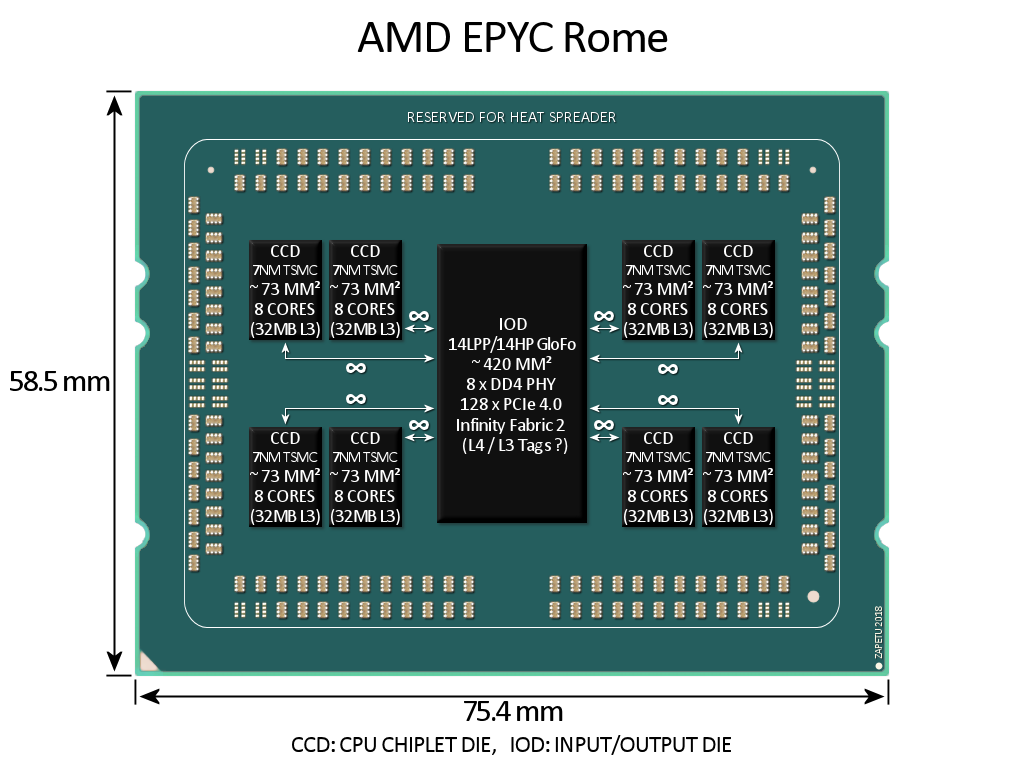
\includegraphics[width=10.24cm]{epyc_rome.png}
  \caption{Un processeur \marque{AMD EPYC Rome}, taille réelle. Il y a 8 \og
    chiplets\fg de 8 coeurs chacuns, physiquement séparés. \label{fig:ROME}}
\end{figure}

Dernier exemple : imaginons deux machines, toujours distantes d'un mètre. Les
deux machines attendent toutes les deux qu'un certain évenement se produise (par
exemple, une intervention d'un utilisateur), et elles veulent déterminer sur
laquelle l'évenement se produit en premier. Pour cela, dès que l'évenement a
lieu sur une machine, elle envoie à l'autre un message sur le réseau disant \og
J'AI GAGNÉ\fg. Le problème, c'est que si les événements ont lieu dans un
intervalle trop court, les messages risquent de se croiser... Et plus les
machines sont éloignées physiquement, plus l'intervalle entre lequel il est
impossible de faire la différence est grand.

\subsection{Accès conflictuels à la mémoire}

Deux accès à la mémoire sont \emph{conflictuels} s'ils ont lieu à la
même adresse et si l'un d'entre eux au moins est une écriture. Dans un
programme séquentiel, on peut permuter deux instructions sans modifier
la sémantique du programme, à conditions qu'elles ne soient pas
conflictuelles. Par exemple, on peut permuter deux lectures, ou bien
deux écritures dans des variables différentes. Les compilateurs se
livrent à ce petit jeu, de même que les processeurs qui font de la
\anglais{out-of-order execution}. Ceci dit, même les processeurs
\anglais{in-order} qui ont un \anglais{pipeline} sont potentiellement
exposés à ces problèmes, car plusieurs instructions sont \og en
vol\fg{} simultanément. De plus, on peut exécuter des opérations
non-conflictuelles \emph{en parallèle}, donc détecter correctement les
conflits permet des formes de parallélisation automatique.

Si on permute deux instructions conflictuelles, trois types de
problème peuvent survenir, qui modifient le résultat de l'exécution du programme :

\begin{tabular}{c||c|c|c}
  \hline
  & Read-After-Write & Write-After-Write & Write-After-Read \\
  & dépendance de données & & anti-dépendance \\
\hline
  & {$\begin{aligned}[t]
  a &= x;\\
  b &= a;
\end{aligned}$}
                                                  &
{$\begin{aligned}[t]
  a &= x;\\
  a &= y;
\end{aligned}$}
                              &
{$\begin{aligned}[t]
  b &= a;\\
  a &= x;\\
\end{aligned}$}
  \\
  \hline
  Effet de la permutation & $b$ incorrect (vieille valeur lue) & $a$ incorrect & $b$ incorrect (nouvelle valeur lue) \\
  \hline
\end{tabular}

Les anti-dépendances (\og \anglais{name dependence}\fg{}) peuvent en
principe être éliminées en introduisant des variables supplémentaires
: il suffirait de remplacer \mintinline{C}{a = x;} par
\mintinline{C}{c = x}; puis remplacer toutes les occurrences suivantes
de $a$ par $c$ pour éliminer le problème.

\subsection{Relations d'ordre sur les évènements dans une machine à mémoire
  partagée}

Lorsqu'un thread s'exécute, des \emph{évènements} ont lieu : lecture/écriture en
mémoire, opération arithmétique, envoi/réception de message sur le réseau, etc.
Indépendamment de leur nature, ces évènements ont lieu dans l'ordre spécifié par
le programme qui s'éxecute (c'est le \og \anglais{program order}\fg). Dans les
machines parallèle, on peut avoir au moins une (prétendue) certitude : les
instructions des programmes séquentiels sont exécutées dans l'ordre. On écrit
$e_1 \po e_2$ pour dire que l'évènement $e_1$ a lieu \emph{avant} $e_2$ dans
l'ordre dicté par le programme.

% Il y a une deuxième chose dont on peut être sûr : un message qui transite sur le
% réseau est forcément émis avant d'être reçu. Ainsi, si $e_1$ est l'évènement \og
% envoi du message $M$\fg et $e_2$ est l'évènement \og réception du message
% $M$\fg, alors on écrit $e_1 \net e_2$.

Discutons maintenant plus précisément de l'accès à une mémoire partagée. Les
lectures et les écritures en mémoire effectuées par différents threads peuvent
être concurrentes, mais les opérations qui concernent les mêmes variables ont
lieu dans un certain ordre, qu'on va tâcher de caractériser.

On considère un ensemble de threads
$\mathcal{T} = \left\{ T_0, T_1, \dots, T_m \right\}$. Ils exécutent donc leurs
instructions de manière séquentielle. On utilise la notation suivante, qui est
bien commode, pour les opérations d'accès à la mémoire :
\begin{itemize}
\item On note $W_i(x)a$ l'évènement : \og le thread $T_i$ écrit la valeur $a$ dans la variable
  $x$\fg.
\item On note $R_i(x)b$ l'évènement : \og le thread $T_i$ lit la variable
  $x$ et obtient la valeur $b$\fg.
\end{itemize}

\medskip

Lorsqu'une opération de lecture a lieu en mémoire, la valeur renvoyée est le
résultat de l'exécution d'une certaine opération d'écriture. Si $w = W(x)a$ est
l'écriture qui stocke dans $x$ la valeur lue par une lecture $r = R(x)a$, alors
on dit que $r$ \og \anglais{reads from}\fg $w$ et on écrit $w \rf r$. On peut
affirmer que pour toute lecture $r$, il existe une unique écriture $w$ telle que
$w \rf r$. Si $w \rf r$, alors la lecture a lieu \og après\fg l'écriture.

Une variable ne peut stocker qu'une seule valeur à la fois. Les écritures dans
une même variable ont donc forcément lieu à la suite les unes des autres, dans
un certain ordre (même si cet ordre n'est pas celui qu'on croit). On note
$w_1 \co w_2$ (\og modification order \fg) lorsque $w_1$ et $w_2$ sont des écritures dans
la même variable $x$ et que $w_1$ a lieu \og avant\fg. Si on se restreint aux
évènements d'écriture sur une seule variable, alors la relation $\co$ est un
ordre \emph{total}.

Enfin, si $r$ est une lecture sur une variable $x$ qui a lieu \emph{avant} une
écriture $w$, on note $r \fr w$ (\og \anglais{reads before}\fg). Cela signifie
que la lecture renvoie une valeur qui se trouvait dans $x$ \og avant\fg
l'écriture, donc que l'écriture a forcément lieu \og après\fg. En fait
$r \fr w \overset{\scriptsize def}{=} \exists w'. w' \rf r \wedge w' \co
w$. Alternativement, on peut dire que $\fr = (\rf)^{-1} ; \co$. Le point-virgule
désigne la composition des relations.

Pour résumer, les trois relations indiquent l'ordre dans lequel deux opérations
conflictuelles ont finalement été exécutées, pour chacun des trois types de
conflit possible~:
\begin{center}
\begin{tabular}{|c|rcl|}
  \hline
  Read-after-Write (RAW)  & $w$ & $\rf$ & $r$ \\
  \hline
  Write-after-Write (WAW) & $w$ & $\co$ & $w$ \\
  \hline
  Write-after-Read (WAR)  & $r$ & $\fr$ & $w$ \\
  \hline
\end{tabular}
\end{center}

Il ne sert à rien d'ordonner les lectures entre elles, puisqu'elles ne sont pas
conflictuelles. %Toutes ces relations sont transitives (c.a.d. que
%$u \rightarrow v$ et $v \rightarrow w$ impliquent $u \rightarrow w$, pour
%chacune des relations considérées).

En présence d'un programme séquentiel, les relations $\rf, \mo$ et $\rb$
coïncide avec $\po$ : toutes les opérations qui ont lieu ont lieu dans l'ordre
indiqué par le programme séquentiel exécuté (les processeurs et les compilateurs
le garantissent en principe). Mais ceci n'est plus vrai en présence de plusieurs
threads. Par exemple :

\begin{center}
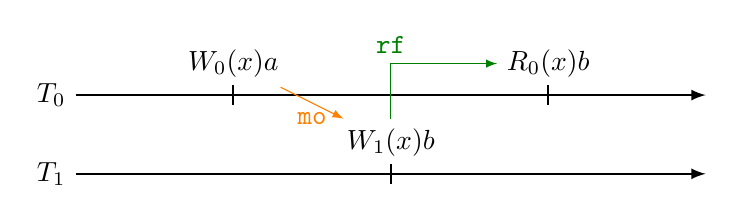
\begin{tikzpicture}[>=latex]
\foreach \i in {0,1}
  \draw[thick, ->] (0,1-\i) node[left] {$T_\i$} -- +(8,0);

\foreach \i / \j in {1/1, 2/0, 3/1}
  \draw[thick] (2*\i,\j) +(0,0.125) -- +(0, -0.125);

\node[above=1mm] at (6,1) (rx) {$R_0(x)b$};
\node[above=1mm] at (4,0) (w1x) {$W_1(x)b$};
\node[above=1mm] at (2,1) (w0x) {$W_0(x)a$};

\draw[Green,->] (w1x) |- node[above] {\tt rf} (rx);
\draw[orange,->] (w0x) -- node[below] {\tt mo} (w1x);

\end{tikzpicture}
\end{center}

On a bien $W_0(x)a \po R_0(x)b$ pour $T_0$, et en présence d'un seul thread on
devrait avoir $W_0(x)a \rf R_0(x)a$, mais à cause de l'écriture effectuée par
$T_1$ la valeur lue n'est plus la bonne, et donc on n'a \emph{pas}
$W_0(x)a \rf R_0(x)b$. Dans cet exemple précis on a
\[
  W_0(x)a \co W_1(x)b \rf R_0(x)b.
\]


\subsection{Formalisation des opérations atomiques}

Jusque-là, on a parlé de lectures et d'écritures. Mais comment exprimer ce que
fait :
\begin{myfilet}
  \begin{minted}{C}
#pragma omp atomic update
c += 10;
\end{minted}
\end{myfilet}
Ce genre d'opération \emph{read-modify-write} n'est pas très naturellement saisi
par le cadre défini jusque-là. On décompose donc la mise à jour en deux opérations :
une lecture (\mintinline{C}{tmp = c;}) puis une écriture (\mintinline{C}{c = tmp + 10;}).

Il reste à faire respecter le caractère atomique de la mise à jour. Pour cela,
il faut imposer qu'aucune autre opération écriture sur $c$ ne vienne
s'interposer entre la lecture et l'écriture. Pour cela, on introduit une
relation spéciale $\rmw$ qui connecte entre elles la lecture et l'écriture qui
constituent une opération de mise à jour atomique telle que \texttt{atomic
  update} ou \texttt{atomic capture}.

Le caractère atomique des opérations est garanti si :
\[
  \rmw \cap (\rb ; \mo) = \emptyset. \tag{\textsc{Atomicity}}
\]
Autrement dit, si on a une mise à jour atomique $r \rmw w$, alors il ne doit pas
y avoir d'autre écriture $w'$ qui s'incruste entre $r$ et $w'$ (et qui entraîne
donc $r \rb w' \mo w$).

Pour illustrer tout ceci, considérons deux mises à jour concurrentes :
\begin{center}
\begin{tabular}{|c|p{2.5cm}||p{2.5cm}|}
  \hline
  État initial : & \multicolumn{2}{c|}{x = 1} \\
  \hline
                 & \tt a = x;     & \tt b = x; \\
                 & \tt x = a + 1; & \tt x = b * 10; \\
  \hline
  Comportement attendu : & \multicolumn{2}{c|}{$x = 11$ ou $x = 20$} \\
  \hline
\end{tabular}
\end{center}

Est-ce que ceci peut produire $x = 2$ ? Ça pourrait être le cas si les
opérations s'entrelaçaient mal, par exemple si les deux lectures avaient lieu
avant les deux écritures. La situation est alors la suivante :

\begin{center}
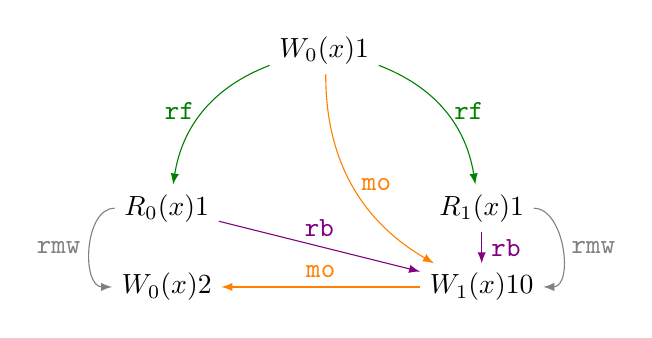
\begin{tikzpicture}[>=latex]
  \node at (0, 2) (init) {$W_0(x)1$};
  
  \node at (-2,0)  (R0) {$R_0(x)1$};
  \node at (-2,-1) (W0) {$W_0(x)2$};

  \node at (2,0)  (R1) {$R_1(x)1$};
  \node at (2,-1) (W1) {$W_1(x)10$};

\draw[Green,->] (init) edge[bend right]  node[left] {\tt rf} (R0);
\draw[Green,->] (init) edge[bend left]  node[right] {\tt rf} (R1);

%\draw[orange,->] (init) edge[bend left]  node[left] {\tt mo} (W0);
\draw[orange,->] (init) edge[bend right]  node[right] {\tt mo} (W1);
\draw[orange,->] (W1) edge[]  node[above] {\tt mo} (W0);

 \draw[Purple,->] (R0) edge  node[above] {\tt rb} (W1);
 \draw[Purple,->] (R1) edge  node[right] {\tt rb} (W1);

 \draw[gray,->] (R0) edge[out=180, in=180]  node[left] {\tt rmw} (W0.west);
 \draw[gray,->] (R1) edge[out=0, in=0]  node[right] {\tt rmw} (W1.east);
\end{tikzpicture}
\end{center}

Mais alors la règle (\textsc{Atomicity}) est mise en défaut, car on a à la fois
\[
  R_0(x)1 \rmw W_0(x)2 \qquad\text{et}\qquad R_0(x)1 \rb W_1(x)10 \mo W_0(x)2.
\]

\subsection{Définition de la \anglais{Sequential Consistency}}
\label{sec:sequential-consistency}

On a vu qu'en parallèle, la \anglais{strict consistency} n'est plus
respectée. Que se passe-t-il si deux \anglais{threads} qui s'exécutent
simultanément sur deux coeurs différents décident d'écrire à la même adresse
mémoire en même temps ?

Forcément, un certain \emph{non-déterminisme} va apparaître, et l'un
des deux coeurs va \og gagner la course\fg. On a vu au
chapitre~\ref{chap:omp} qu'il est nécessaire, pour garantir la
sémantique du code, de protéger les accès concurrents aux variables
partagées par des sections critiques, des opérations atomiques ou
encore des verrous. Ces mécanismes garantissent au programmeur que
tout se passera comme si les accès aux variables partagées avaient
lieu séquentiellement. Si plusieurs threads sont en compétition pour
entrer dans une section critique, il vont y parvenir les uns à la
suite des autres, mais \emph{dans un certain ordre}, qui n'est pas
spécifié et qui peut dépendre du matériel, de l'OS ou encore de
l'environnement d'exécution.

Ceci est assez bien capturée par la notion que Leslie Lamport a appelé la
\anglais{Sequential Consistency}~\cite{Lamport79}. Un système parallèle possède
cette propriété si, bien que les accès à la mémoire des différents threads
soient concurrents, tout se passe comme si les opérations de lecture/écriture
dans la mémoire étaient exécutées de manière séquentielle.

En particulier, tous les threads observent les écritures vers la mémoire dans le
même ordre, et donc ont la même \og vision\fg de l'état de la mémoire. Les accès
mémoire des threads peuvent s'entrelacer arbitrairement, mais tous les threads
doivent percevoir le même ordre sur les opérations.

\begin{myexample}
  Considérons quatre threads qui font des opérations sur des variables
  partagées.
\begin{center}
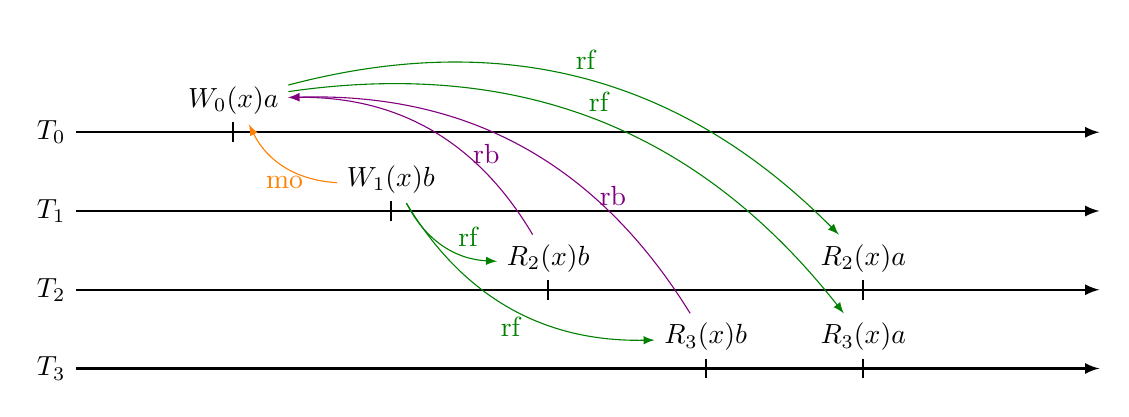
\begin{tikzpicture}[>=latex]
\foreach \i in {0,1,2,3}
  \draw[thick, ->] (0,3-\i) node[left] {$T_\i$} -- +(13,0);

\foreach \i / \j in {4/0, 5/0, 3/1, 5/1, 2/2, 1/3}
  \draw[thick] (2*\i,\j) +(0,0.125) -- +(0, -0.125);

\node[above=1mm] at (8,0) (r3b) {$R_3(x)b$};
\node[above=1mm] at (10,0) (r3a) {$R_3(x)a$};
\node[above=1mm] at (6,1) (r2b) {$R_2(x)b$};
\node[above=1mm] at (10,1) (r2a) {$R_2(x)a$};
\node[above=1mm] at (4,2)  (w1) {$W_1(x)b$};
\node[above=1mm] at (2,3) (w0) {$W_0(x)a$};

\draw[Green,->] (w0) edge[bend left] node[above] {rf} (r2a);
\draw[Green,->] (w0) edge[bend left] node[above] {rf} (r3a);

\draw[Green,->] (w1) edge[bend right] node[above, near end] {rf} (r2b);
\draw[Green,->] (w1) edge[bend right] node[below] {rf} (r3b);

\draw[orange,->] (w1) edge[bend left] node[below] {mo} (w0);

\draw[Purple,->] (r2b) edge[bend right] node[above, near start] {rb} (w0);
\draw[Purple,->] (r3b) edge[bend right] node[above, near start] {rb} (w0);


\end{tikzpicture}
\end{center}

Ici, le comportement du système n'est manifestement pas régi par la
\anglais{strict consistency} : comme $W_0(x)a$ a lieu \og avant\fg $W_1(x)b$, on
ne devrait pas voir réapparaître la valeur $a$ dans la variable $x$ par la suite
(or $T_2$ et $T_3$ observent ceci). Tout se passe pourtant comme si les
opérations avaient eu l'une après l'autre dans l'ordre suivant :
\[
W_1(x)b ~ < ~  R_2(x)b ~ < ~  R_3(x)b ~ < ~ 
W_0(x)a ~ < ~  R_2(x)a ~ < ~  R_3(x).
\]
Ce que les threads observent pourrait être causé par un ordonnanceur
(maléfique...) qui aurait retardé l'exécution de $T_0$ pour que $W_0(x)a$ tombe
pile au mauvais moment, entre les deux lectures de $T_3$. Le système est
néanmoins séquentiellement consistant car tout se passe comme si les accès
mémoire avaient lieu séquentiellement dans un ordre raisonnable.
\end{myexample}

Essayons de rendre ça à peu près formel. Une \important{exécution} $E_i$ d'un
thread $T_i$ décrit l'ensemble des évènements de lecture/écriture de la mémoire
(avec les valeurs associées) dont $T_i$ a commandé l'exécution.

Un système parallèle possède la \anglais{sequential consistency} (il est \og
séquentiellement consistent\fg) si, pour chacune des exécutions possibles des
threads auxquelles il peut aboutir, on peut construire un \emph{historique},
c'est-à-dire une séquence totalement ordonnée $H$ qui contient une et une seule
fois chaque évènements de l'ensemble des exécutions $E_1, \dots, E_n$. De
manière équivalente, cela revient à dire qu'il y a une relation d'ordre totale
$<$ sur les évènements. Cette relation/cet historique (c'est la même chose) doit
respecter deux contraintes :
\begin{enumerate}
\item Compatibilité avec le \anglais{program order} : si $e_1 \po e_2$, alors
  $e_1 < e_2$ dans l'historique.

\item Cohérence de la mémoire : toute lecture d'une variable $x$
  doit renvoyer la valeur écrite par l'évènement d'écriture sur $x$ le plus
  récent dans l'historique.
\end{enumerate}

\medskip

\paragraph{Définition alternative} Une définition alternative très pratique de
la \anglais{sequential consistency} consiste à dire que la relation
$\po \cup \rf \cup \co \cup \fr$ doit être acyclique.

Les deux définitions sont équivalentes : si on dispose d'un historique, on peut
en déduire facilement les relations $\rf, \co, \fr$, qui sont alors acycliques
par définition --- Si $\po \cup \rf \cup \co \cup \fr$ est acyclique, alors
c'est un ordre partiel, qui peut se compléter en un ordre total [via un tri
topologique] et ceci donne l'historique).

\subsection{La \anglais{sequential consistency} est désirable}
\label{sec:peterson-proof}

L'environnement d'exécution d'\OMP garantit que les accès \emph{atomiques} à des
variables partagés (via \texttt{omp atomic}) sont séquentiellement consistants.

Même si elle tolère un certain non-déterminisme, la \anglais{sequential
  consistency} est une caractéristique souhaitable, et elle permet de faire des
raisonnements assez simples sur la correction des programmes multi-threads.  Par
exemple, considérons un mécanisme d'exclusion mutuelle pour deux threads, le
\anglais{Peterson lock}~\cite{Peterson81}.

\begin{myfilet}
\begin{minted}{C}
bool flag[2];
int victim;

void lock() 
{
	int i = omp_get_thread_num();
	int j = 1 - i;
	flag[i] = true;                            // I'm interested
	victim = i;                                // you go first
	while (victim == i && flag[j] == true) {}; // wait
}

void unlock() 
{
	int i = omp_get_thread_num();
	flag[i] = false; // I'm not interested
}
\end{minted}
\end{myfilet}

\begin{theorem}
  Si la machine est séquentiellement consistante, alors le \anglais{Peterson
    lock} garantit l'exclusion mutuelle entre deux threads.
\end{theorem}

\begin{myproof}
  Raisonnons par l'absurde, et supposons que ce ne soit pas le cas. Cela
  signifie que les deux threads $T_0$ et $T_1$ peuvent parvenir à exécuter la
  fonction \mintinline{C}{lock()}, à en sortir tous les deux et à se retrouver
  tous les deux dans la section critique (CS) simultanément. Chaque thread
  exécute donc la séquence d'opérations :
  \begin{align*}
    T_0 &: W_0(\mintinline{C}{flag[0]}) \mintinline{C}{true} \po  W_0(\mintinline{C}{victim}) 0 \po R_0(\mintinline{C}{victim}) ?  \po  R_0(\mintinline{C}{flag[1]}) ? \po CS_0 \\
    T_1 &: W_1(\mintinline{C}{flag[1]}) \mintinline{C}{true} \po  W_1(\mintinline{C}{victim}) 1  \po R_1(\mintinline{C}{victim}) ? \po R_1(\mintinline{C}{flag[0]}) ? \po CS_1
  \end{align*}
  Supposons, sans perte de généralité, qu'au moment où les deux threads se
  trouvent dans la section critique, le thread 0 était le dernier à écrire dans
  \texttt{victim} :
  \[
    W_1(\mintinline{C}{victim}) 1 \co W_0(\mintinline{C}{victim}) 0.
  \]
  Ceci implique que $T_0$ a observé \mintinline{C}{victim == 0} dans la
  condition de la boucle (il n'y a plus d'autre écriture dans \texttt{victim} et
  $T_0$ doit lire la dernière valeur écrite --- plus précisément, on aurait un
  défaut de \emph{sequential consistency} avec un cycle si ce n'était pas le
  cas). Puisque $T_0$ est entré dans la section critique, c'est forcément qu'il
  a également observé \mintinline{C}{flag[1] == false}. Par conséquent, on a :
  \[
    W_0(\mintinline{C}{victim}) 0 \po R_0(\mintinline{C}{victim}) 0 \po R_0(\mintinline{C}{flag[1]}) \mintinline{C}{false}.
  \]
  En combinant tout ce qu'on sait, on trouve que :

  \begin{center}
  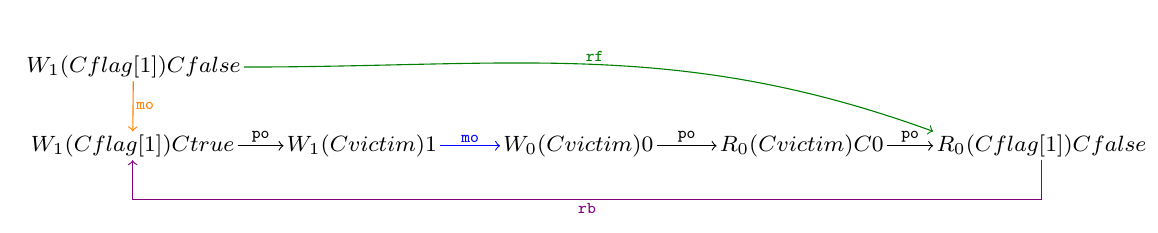
\begin{tikzpicture}[every node/.style={font=\footnotesize, inner sep=1pt}]
    \path[use as bounding box] (0, -0.75) rectangle (14, 1.5);
    \node[anchor=west] at (-0.06, 1) (Winit) { $W_1(\mintinline{C}{flag[1]}) \mintinline{C}{false}$ };
    \node[anchor=west] at (0, 0) (Wflag) { $W_1(\mintinline{C}{flag[1]}) \mintinline{C}{true}$ };
    %\po
    \node[anchor=west] at (3.25, 0) (Wvictim1) { $W_1(\mintinline{C}{victim}) 1$ };
    % \co
    \node[anchor=west] at (6, 0) (Wvictim0) { $W_0(\mintinline{C}{victim}) 0$};
    % \po
    \node[anchor=west] at (8.75, 0) (Rvictim) { $R_0(\mintinline{C}{victim}) \mintinline{C}{0}$};
    % \po
    \node[anchor=west] at (11.5, 0) (Rflag) { $R_0(\mintinline{C}{flag[1]}) \mintinline{C}{false}$};

    \draw[orange] (Winit) edge[->] node[right] {$\scriptstyle \tt mo$} (Wflag);
    \draw (Wflag) edge[->] node[above] {$\scriptstyle \tt po$} (Wvictim1);
    \draw[blue] (Wvictim1) edge[->] node[above] {$\scriptstyle \tt mo$} (Wvictim0);
    \draw (Wvictim0) edge[->] node[above] {$\scriptstyle \tt po$} (Rvictim);
    \draw (Rvictim) edge[->] node[above] {$\scriptstyle \tt po$} (Rflag);

    
    \draw[Green] (Winit.east) edge[out=0,in=160,->] node[above] {$\scriptstyle \tt rf$} (Rflag.north west);

    \draw[Purple,->] (Rflag.south) -- +(0, -0.5) -| node[below,near start] {$\scriptstyle \tt rb$} (Wflag.south);
  \end{tikzpicture}
\end{center}

  % \[
  %   W_1(\mintinline{C}{flag[1]}) \mintinline{C}{true} \po W_1(\mintinline{C}{victim}) 1
  %   \co W_0(\mintinline{C}{victim}) 0 \po R_0(\mintinline{C}{flag[1]}) \mintinline{C}{false}.
  % \]



  % En particulier, on a
  % $W_1(\mintinline{C}{flag[1]}) \mintinline{C}{true} \xrightarrow{*}
  % R_0(\mintinline{C}{flag[1]}) \mintinline{C}{false}$, et il n'y a pas d'autre
  % écriture dans \mintinline{C}{flag[1]}. On a donc
  % $W_1(\mintinline{C}{flag[1]})\mintinline{C}{true} \rf R_0(\mintinline{C}{flag[1]})
  % \mintinline{C}{false}$, une incohérence.

  % TODO : exhiber un cycle avec fr.
  On voit un cycle, par conséquent, la machine n'est pas séquentiellement consistente. CQFD.\qed
\end{myproof}

Le \anglais{Peterson lock} est exempt de \anglais{deadlock} : les deux threads
ne peuvent pas rester tous les deux bloqués dans la boucle
\mintinline{C}{while()} car il faudrait que \texttt{victim} vale simultanément 0
et 1. En fait, c'est encore mieux : le \anglais{Peterson lock} est
\anglais{starvation-free} : chaque thread qui tente d'acquérir le verrou fini
par y parvenir en temps fini lorsque l'autre le libère.


\section{Les processeurs modernes ne sont pas \anglais{Sequentially Consistent}}
\label{sec:CPU-not-SC}

Une des raisons fondamentales pour lesquelles le modèle mémoire d'\OMP ne
garantit pas la \anglais{sequential consistency} c'est que... les processeurs ne
la garantissent pas.

Le problème avec la \anglais{sequential consistency}, c'est que ça a un
coût. Maintenir la même vue de la mémoire pour tous les coeurs d'un processeur
serait trop coûteux et trop difficile à mettre en oeuvre. Le problème principal
réside dans la nécessité de devoir rendre simultanément et instantanément
visible à tous les threads chaque écriture. Ceci interdit que les opérations
d'accès à la mémoire puissent se dérouler de façon \og locale\fg à chaque coeur,
sans interaction avec le reste des processeurs. Aussi, lire et écrire en mémoire
nécessiterait forcément des communications et une synchronisation coûteuse pour
maintenir la \anglais{sequential consistency}.

Sans trop rentrer dans les détails (on y reviendra abondamment au
chapitre~\ref{chap:memory}), les processeurs ont des \emph{caches}. Les coeurs
ont généralement des caches \og privés\fg dont le contenu n'est pas visible par
les autres coeurs. Lorsqu'un thread écrit une valeur dans une variable $x$, en
réalité seul son cache privé est mis à jour, du moins dans un premier temps. À
un moment indéterminé du futur, lorsqu'il faudra faire de la place dans le cache
pour d'autres données plus récentes, l'adresse contenant $x$ sera évincée du
cache et (peut-être) écrite dans la mémoire. Pendant toute une période, le coeur
qui écrit $x$ a une vision de la mémoire différente des autres, dans laquelle
$x$ a la nouvelle valeur. Or ceci est précisément interdit par la
\anglais{sequential consistency}.

\begin{danger}
  Ceci est vrai si le cache est \anglais{write-back}. Mais de toute façon, même
  s'il est \anglais{write-through}, il va y avoir un délai non-négligeable de
  propagation de l'écriture jusqu'à la RAM.
\end{danger}

Du coup, les processeurs modernes n'offrent pas la \anglais{sequential consistency}.

\subsection{La \anglais{sequential consistency} est trop coûteuse}

Voici un argument formel qui démontre que dans un système séquentiellement
consistant, les opérations d'accès à la mémoire ne peuvent pas être
rapides. Considérons un système à deux processeurs, et notons $\tau$ la
\emph{latence} des communications entre eux (c'est le temps minimal nécessaire
pour transférer des informations entre eux). Si $d$ désigne la distance qui les
sépare, alors il semble raisonnable de supposer que $\tau \geq d/c$, où $c$
désigne la vitesse de la lumière. Par ailleurs, on a aussi que
$\tau \geq \rho l$, où $\rho$ désigne le temps nécessaire pour franchir un
transistor et $l$ désigne le nombre de transistors sur le parcours. Cette
deuxième borne est a priori plus forte que la première.

Le résultat suivant figure dans~\cite{Lipton1988PramAS}. \medskip

\begin{theorem}\label{thm:sc_slow}
  Notons $r$ et $w$ les temps nécessaire pour effectuer des opérations de
  lecture et d'écriture \emph{dans le meilleur des cas} sur chacun des deux
  processeurs. Si le système composé des deux processeurs est séquentiellement
  consistant, alors $r + w \geq \tau$.
\end{theorem}

\begin{myproof}
  Considérons deux threads qui accèdent à quatre variables partagées $x, y, w$
  et $z$, initialement égales à zéro, et qui s'exécutent sur chacun des deux
  processeurs. Les deux threads exécutent les programmes suivants:
  \begin{align*}
    T_0 &: W_0(x)1 \po R_0(y) w \\
    T_1 &: W_1(y)1 \po R_0(x) z
  \end{align*}
  Comme la machine est séquentiellement consistante, il est impossible d'avoir
  $(w,z) = (0, 0)$ à la fin de l'exécution du programme. En effet, pour obtenir
  $w=0$, il faut que $R_0(y)0 \fr W_1(y)1$. Mais alors comme les deux threads
  effectuent leurs opérations dans l'ordre, on devrait avoir
  \[
    W_0(x)1 \po R_0(y) 0 \fr W_1(y)1 \po R_0(x) z,
  \]
  On a donc $W_0(x)1 \rf R_0(x) z$, donc $z=1$.

  Maintenant, supposons que les deux threads exécutent leurs opérations de
  manière synchrone et que $r+w < \tau$. Aucun des deux processeurs ne peut
  alors \og percevoir\fg l'écriture que l'autre a effectué, car il ne s'est pas
  écoulé assez de temps pour que l'information lui parvienne. La seule issue
  possible est alors $(w,z) = (0, 0)$, une contradiction. Ceci démontre que
  $r+w \geq \tau$. \qed
\end{myproof}

\subsection{Validation expérimentale du défaut de \anglais{Sequential Consistency}}

Il est possible de démontrer expérimentalement qu'un ordinateur moderne
multi-coeurs n'est pas séquentiellement consistant. Essayons de tester le
\anglais{Peterson lock} (tous les tests ont lieu sur un laptop normal) :

\begin{myfilet}
\begin{minted}{C}
int x = 0;
#pragma omp parallel for num_threads(2)
for (int i = 0; i < 10000000; i++) {
	lock();
	x++;
	unlock();
}
printf("x : %10u\n", x);
\end{minted}
\end{myfilet}

\paragraph{Premier essai} Les deux threads restent coincés indéfiniment dans la
fonction \mintinline{C}{lock()}, ce qui semble contredire l'affirmation que le
\anglais{Peterson lock} est \anglais{deadlock-free}.

C'est la faute du compilateur : il suppose que les variables \texttt{flag} et
\texttt{victim} ne sont pas modifiées de manière extérieure. Du coup
l'optimiseur retire le test \mintinline{C}{victim == i} de la condition de la
boucle, car il \og sait\fg qu'il est vrai. La boucle devient alors
\mintinline{C}{while(true) {}} et ça bloque le programme.

\begin{danger}
  Voici le code assembleur, avec la boucle infinie bien visible en bas.
  \begin{myfilet}
\begin{minted}{asm}
lock:
	pushq   %rbx
	call    omp_get_thread_num@PLT
	movslq  %eax, %rdx           ; %rdx == i
	leaq    flag(%rip), %rax     ; %rax == adresse de flag
	movq    %rdx, %rbx           ; %rbx == i
	movb    $1, (%rax,%rdx)      ; flag[i] = true
	movl    %edx, victim(%rip)   ; victim = i
	movl    $1, %edx             ; 
	subl    %ebx, %edx           ; 
	movslq  %edx, %rdx           ; j = i - 1
	cmpb    $0, (%rax,%rdx)      ; if flag[j] = 0...
	je      critical             ; ... then goto CS ...
loop:
	jmp     loop                 ; ... else goto loop ...
\end{minted}
  \end{myfilet}
\end{danger}%$

Pour empêcher le compilateur d'effectuer cette optimisation, on a deux solutions
: désactiver toutes les optimisations (compiler avec \texttt{-O0}), ou bien
déclarer que les variables \texttt{flag} et \texttt{victim} peuvent être
modifiées extérieurement, donc qu'elles sont \mintinline{C}{volatile}.

\paragraph{Deuxième essai} On modifie le code en ajoutant :
\begin{myfilet}
\begin{minted}{C}
volatile bool flag[2];
volatile int victim;
\end{minted}
\end{myfilet}

Ceci permet au programme de s'exécuter et le résultat est :
\begin{verbatim}
x :    9999827
\end{verbatim}

Cette fois, l'acquisition du verrou termine en temps fini, mais il semble que
l'exclusion mutuelle ne soit pas garantie : on retrouve en apparence un
phénomène de non-atomicité des incrémentations.

\paragraph{Troisième essai} Il est facile de vérifier explicitement si les deux
threads se trouvent ou pas en même temps dans la section critique. Modifions les
deux fonctions de la façon suivante :
\begin{myfilet}
\begin{minted}{C}
volatile int inside_cs = -1;

void lock() 
{
	int i = omp_get_thread_num();
	int j = 1 - i;
	flag[i] = true;                    // I'm interested
	victim = i;                        // you go first
	while (victim == i && flag[j]) {}; // wait
        assert(inside_cs == -1);           // critical section must be empty
	inside_cs = i;                     // now I'm in the critical section
}

void unlock() 
{
	int i = omp_get_thread_num();
	assert(inside_cs == i);            // I was in the critical section, not the other one
	inside_cs = -1;                    // now the critical section is empty
	flag[i] = false;                   // I'm not interested
}
\end{minted}
\end{myfilet}

Et voici le résultat, prévisible :
\begin{verbatim}
lock: Assertion `inside_cs == -1' failed.
\end{verbatim}

Nous avons prouvé mathématiquement que le \anglais{Peterson lock} garantit
l'exclusion mutuelle sur les machines séquentiellement consistantes ;
l'exclusion mutuelle n'est manifestement pas garantie ; conclusion : un laptop
\marque{x86-64} n'offre \emph{pas} la \anglais{sequential consistency}.

\subsection{Une des causes : le \og \anglais{Store Buffering}\fg}

On peut pointer le problème plus précisément. Le programme suivant démontre
explicitement un défaut de \anglais{sequential consistency}. En fait, c'est le
même programme utilisé dans la preuve du théorème~\ref{thm:sc_slow}. Il compte
le nombre de fois où le processeur exhibe un comportement incompatible avec la
\anglais{sequential consistency}. Deux threads partagent deux variables. Ils en
écrivent une \emph{puis} lisent l'autre. La question est de savoir s'il peuvent
lire tous les deux les valeurs initiales des deux variables (si la machine était
séquentiellement consistante ce serait impossible, comme on l'a vu).

\begin{center}
\begin{tabular}{|c|p{2cm}||p{2cm}|}
  \hline
  État initial : & \multicolumn{2}{c|}{x = 0 ; y = 0} \\
  \hline
  & \tt x = 1; & \tt y = 1; \\
  & \tt a = y; & \tt b = x; \\
  \hline
  Comportement relâché : & \multicolumn{2}{c|}{a = 0 ; b = 0} \\
  \hline
\end{tabular}
\end{center}

Ceci est en fait analogue à l'algorithme d'\og exclusion mutuelle du pauvre\fg{}
de la section~\ref{sec:relaxed-behaviors}. Cet exemple s'appelle SB dans la
littérature spécialisée.

\begin{myfilet}
\begin{minted}{C}
int relaxed = 0;
int x, y, w, z;

#pragma omp parallel num_threads(2)
{
	int i = omp_get_thread_num();
	for (int j = 0; j < 10000000; j++) {
		#pragma omp master
		x = y = 0;

                #pragma omp barrier
		if (i == 0) {
			x = 1;
			w = y;
		} else {	
			y = 1;
			z = x;
		}
	        #pragma omp barrier

                #pragma omp master
		if (z == 0 && w == 0)
			relaxed++;
	}
}
printf("relaxed behavior = %d\n", relaxed);
\end{minted}  
\end{myfilet}

Résultat de l'exécution (laptop \marque{x86-64}) :
\begin{verbatim}
Relaxed behavior = 1561
\end{verbatim}

Quand on observe le comportement \og relaché\fg, ce qui se passe est décrit par
le diagramme suivant~:

\begin{center}
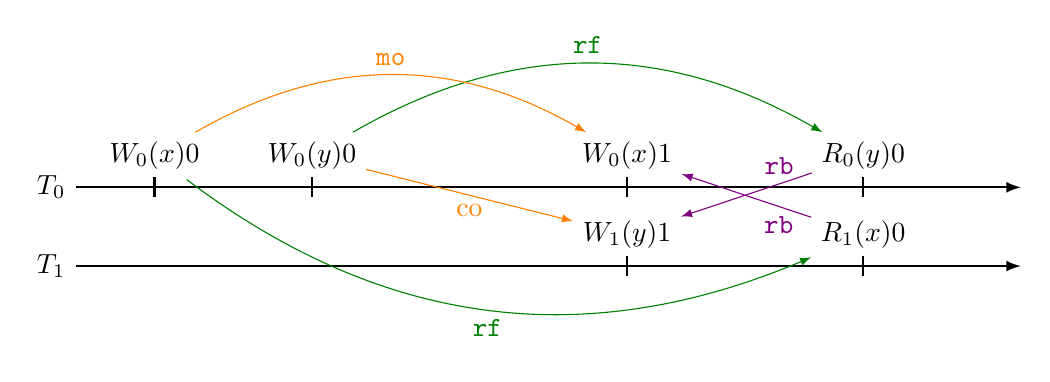
\begin{tikzpicture}[>=latex]
\foreach \i in {0,1}
  \draw[thick, ->] (0,1-\i) node[left] {$T_\i$} -- +(12,0);

\foreach \i / \j in {1/1, 3/1, 7/1, 10/1, 7/0, 10/0}
  \draw[thick] (\i,\j) +(0,0.125) -- +(0, -0.125);

\node[above=1mm] at (1,1) (initx) {$W_0(x)0$};
\node[above=1mm] at (3,1) (inity) {$W_0(y)0$};


\node[above=1mm] at (7,1)  (wx) {$W_0(x)1$};
\node[above=1mm] at (10,1) (ry) {$R_0(y)0$};
\node[above=1mm] at (7,0)  (wy) {$W_1(y)1$};
\node[above=1mm] at (10,0) (rx) {$R_1(x)0$};

\draw[Green,->] (inity) edge[bend left]  node[above] {\tt rf} (ry);
\draw[Green,->] (initx) edge[bend right] node[below] {\tt rf} (rx);

\draw[orange,->] (inity) edge  node[below] {co} (wy);
\draw[orange,->] (initx) edge[bend left] node[above] {\tt mo} (wx);

\draw[Purple,->] (ry) edge node[above, near start] {\tt rb} (wy);
\draw[Purple,->] (rx) edge node[below, near start] {\tt rb} (wx);
\end{tikzpicture}
\end{center}

Il y a violation de SC. On le voit à cause du cycle
$W_0(x)1 \po R_0(y)0 \fr W_1(y)1 \po R_1(x)0 \fr W_0(x)1$.


\begin{danger}
Un examen du code assembleur produit par \marque{gcc 8.3.0} démontre que le
compilateur s'est permis d'entrelacer les lectures et les écritures.
\begin{myfilet}
\begin{minted}{asm}
T_0:
	movq    $0, 8(%rbx)             ; x = 0
	movq    $0, (%rbx)              ; y = 0
	call    GOMP_barrier@PLT
	movq    8(%rbx), %rax           ; %rax = y
	movq    $1, (%rbx)              ; x = 1
	movq    %rax, 16(%rbx)          ; w = %rax
	orq     24(%rbx), %rax          ; if (w != 0 || z != 0) then ...
	jne     skip                    ; ... goto skip
	addl    $1, 32(%rbx)            ; n++
skip:
	subl    $1, %ebp                ; i--
        jne     T_0                     ; if (i != 0) goto T_0

T_1:

	call    GOMP_barrier@PLT
	movq    (%rbx), %rax            ; %rax = x
	movq    $1, 8(%rbx)             ; y = 1
	movq    %rax, 24(%rbx)          ; z = %rax
	subl    $1, %ebp                ; i--
	jne     T_1                     ; if (i != 0) goto T1
\end{minted}
\end{myfilet}%$

On peut l'empêcher en écrivant :
\begin{myfilet}
\begin{minted}{C}
x = 1;
asm volatile("" ::: "memory");  // ne fait rien mais prétend modifier arbitrairement la mémoire
w = y;
...	
y = 1;
asm volatile("" ::: "memory");  // ne fait rien mais prétend modifier arbitrairement la mémoire
z = x;
\end{minted}
\end{myfilet}

Et on obtient alors le code assembleur attendu :
\begin{myfilet}
\begin{minted}{asm}
T_0:
...
        movq    $1, (%rbx)              ; x = 1
	movq    8(%rbx), %rax           ; %rax = y
	movq    %rax, 16(%rbx)          ; w = y
...
T_1:
...
        movq    $1, 8(%rbx)             ; y = 1
	movq    (%rbx), %rax            ; %rax = x
	movq    %rax, 24(%rbx)          ; z = x
...
\end{minted}
\end{myfilet}

Résultat :
\begin{verbatim}
Relaxed behavior = 1296
\end{verbatim}

C'est bien le processeur qui est coupable, et pas le compilateur qui fait
n'importe quoi.
\end{danger}

En fait, ce comportement est \og normal\fg. Les manuels des processeurs
\marque{x86} le documentent et expliquent que chaque thread matériel possède une
\important{file} d'écritures vers la mémoire (le \og \anglais{Store
  Buffer}\fg). L'intérêt, c'est qu'un thread matériel n'a pas besoin d'attendre
que l'écriture soit complète pour commencer à exécuter les instructions
suivantes. Les écritures qui sont dans la file sont effectuées dans l'ordre. Un
processeurs Intel contemporain possède un \anglais{Store Buffer} capable de
contenir 40-50 écritures.

Pour lire le contenu de la mémoire à une adresse $x$, un thread matériel examine
d'abord sa file d'écriture : si une écriture en attente vers l'adresse $x$,
alors la lecture renvoie la dernière valeur qui devrait être écrite en
$x$. Sinon, on va lire la mémoire à l'adresse $x$ (cf. fig.~\ref{fig:tso}).

\begin{figure}
  \centering
  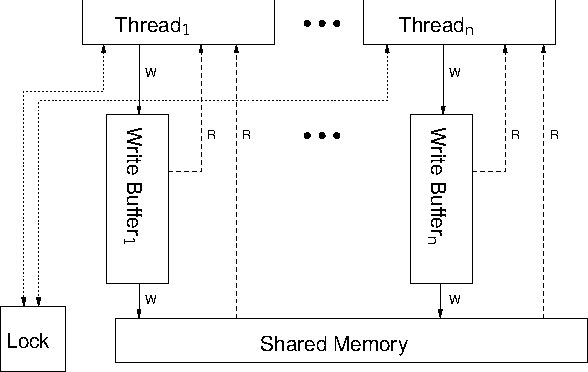
\includegraphics[width=0.75\textwidth]{tso}
  \caption{Le fonctionnement des architectures TSO (image~:~A Tutorial
    Introduction to the ARM and POWER Relaxed Memory Models) \label{fig:tso}}
\end{figure}

Voici comment le \anglais{Store Buffering} explique que le processeur ne soit
pas séquentiellement consistant, comme mis en évidence par l'expérience
précédente : le thread $T_0$ fait \mintinline{C}{x = 1}, c'est-à-dire qu'il
enfile l'écriture de $x$ dans sa file d'écriture. Il lit ensuite la valeur de
$y$ en mémoire (qui est alors 0, $T_1$ est en retard). Puis, plus tard, les
écritures en attente sont finalement exécutées, donc les autres thread
percevront $x=1$... mais entre temps $T_1$, qui s'est réveillé, a eu le temps de
lire $x=0$ en mémoire.

Les machines qui implémentent cette architecture possèdent la propriété du
\anglais{Total Store Ordering} (TSO). Dans les processeurs TSO, un thread
perçoit ses propres écritures \emph{avant} qu'elles ne soient visibles par les
autres threads. Par contre, les écritures d'un thread sont perçues par tous les
\emph{autres} threads simultanément. Ce n'est pas aussi bien que la
\anglais{sequential consistency} mais ce n'est pas si mal. Les processeurs
\marque{SPARC} ont aussi cette caractéristique.

\subsection{Peut-on synchroniser des threads ? Le \og Message Passing\fg}

Essayons de synchroniser et de faire communiquer deux threads sans utiliser de
mécanisme spécial. Le thread $T_0$ effectue un calcul; une fois que le résultat
est prêt, $T_0$ informe $T_1$ qui récupère la valeur en question. Pour cela, un
\anglais{flag} qui vaut initialement 0 passe à 1 lorsque les données sont
prêtes. $T_1$ attend activement que ce \anglais{flag} passe à 1 puis récupère
les données.

\begin{center}
\begin{tabular}{|c|p{2cm}||p{2cm}|}
  \hline
  État initial : & \multicolumn{2}{c|}{x = 0 ; y = 0} \\
  \hline
  & \tt x = 1; & \tt a = y; \\
  & \tt y = 1; & \tt b = x; \\
  \hline
  Comportement relâché : & \multicolumn{2}{c|}{a = 1 ; b = 0} \\
  \hline
\end{tabular}
\end{center}

Le test est répété plusieurs fois, avec des flags et des données différentes,
prises dans un ordre pseudo-aléatoire. Il s'appelle MP dans la littérature spécialisée.

\begin{myfilet}
\begin{minted}{C}
#include <stdio.h>
#include <stdlib.h>
#include <omp.h>

int main()
{
	int relaxed = 0;
	int ntest = 1000000;
	volatile int *flag = malloc(ntest * sizeof(*flag));
	int *data = malloc(ntest * sizeof(*data));
	int *shuffle = malloc(ntest * sizeof(*shuffle));

	// setup
	for (int i = 0; i < ntest; i++) {
		flag[i] = data[i] = 0;
                // random-looking permutation of 0, ..., ntest-1
		shuffle[i] = (3 * 7 * i + 0xCAFE) % ntest;
	}

	#pragma omp parallel num_threads(2)
	{
		int i = omp_get_thread_num();
		for (int j = 0; j < ntest; j++) {
			int k = shuffle[j];
			if (i == 0) {
				data[k] = 1;             // write data
				flag[k] = 1;             // flag "data is ready"
			} else {
				while (flag[k] == 0) {}  // busy-wait for flag
				if (data[k] == 0)        // read data
					relaxed++;
			}
		}
	}
	printf("Relaxed behavior = %d\n", relaxed);
}
\end{minted}
\end{myfilet}

La bonne nouvelle, c'est que ceci se comporte correctement sur les architectures
TSO. En effet, comme les écritures sont mis dans une \emph{file} et qu'elles ne
sont pas réordonnées, alors $T_1$ ne peut pas percevoir \mintinline{C}{flag[k] == 1}
sans percevoir aussi \mintinline{C}{data[k] == 1}. La mauvaise nouvelle,
c'est que toutes les architectures ne sont pas TSO : les \marque{ARM} et les
\marque{POWER} ne le sont pas ! Et ça ne loupe pas : sur un \marque{Raspberry Pi
  3B+} on obtient :
\begin{verbatim}
Relaxed behavior = 964
\end{verbatim}

Voici ce qu'on observe :

\begin{center}
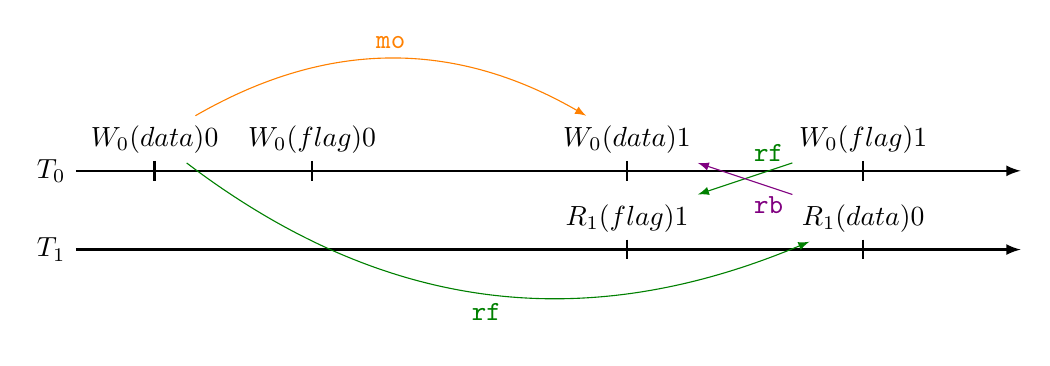
\begin{tikzpicture}[>=latex]
\foreach \i in {0,1}
  \draw[thick, ->] (0,1-\i) node[left] {$T_\i$} -- +(12,0);

\foreach \i / \j in {1/1, 3/1, 7/1, 10/1, 7/0, 10/0}
  \draw[thick] (\i,\j) +(0,0.125) -- +(0, -0.125);

\node[above=1mm] at (1,1) (initx) {$W_0(data)0$};
\node[above=1mm] at (3,1) (inity) {$W_0(flag)0$};


\node[above=1mm] at (7,1)  (wx) {$W_0(data)1$};
\node[above=1mm] at (10,1) (wy) {$W_0(flag)1$};
\node[above=1mm] at (7,0)  (ry) {$R_1(flag)1$};
\node[above=1mm] at (10,0) (rx) {$R_1(data)0$};

\draw[Green,->] (initx) edge[bend right]  node[below] {\tt rf} (rx);
\draw[Green,->] (wy) edge  node[above, near start] {\tt rf} (ry);

\draw[orange,->] (initx) edge[bend left]  node[above] {\tt mo} (wx);

\draw[Purple,->] (rx) edge  node[below, near start] {\tt rb} (wx);
\end{tikzpicture}
\end{center}

Le défaut de SC est démontré par le cycle
$W_0(data)1 \po W_0(flag)1 \rf R_1(flag)1 \po R_1(data)0 \fr W_0(data)1$.

Comment expliquer ceci ? Les écritures effectuées par $T_0$ ont lieu à des
adresses différentes, et donc le processeur pourrait les réordonner et les
effectuer dans le désordre; et/ou elles pourraient être \og propagées\fg à $T_1$
dans le désordre; et/ou les lectures effectuées par $T_1$ pourraient être
réordonnées et réalisées dans l'ordre opposé à celui spécifié par le
programme. Quoi qu'il en soit, on observe qu'il est donc possible de percevoir
certaines écritures tout en ne percevant pas d'autres écritures qui étaient
censées avoir lieu \emph{avant}.

% \subsection{Le \og Write-to-Read Causality\fg}

% Mais en fait, les choses peuvent être encore pire. Différents threads peuvent
% percevoir les écritures dans des ordres différents les uns des autres. Le test
% suivant le met en évidence. C'est la même chose que le précédent (le \og
% \anglais Message Passing}\fg), mais à trois threads :
% \begin{enumerate}
% \item Le thread \#0 signale au thread \# 1 que les données sont prêtes en faisant passer un \anglais{flag} à 1.
% \item Le thread \#1 attend que le \anglais{flag} annonçant la disponibilité des données soit à 1. Puis il définit un second flag à 1.
% \item Le thread \#2 attend que le second \anglais{flag} passe à 1, puis il lit les données.
% \end{enumerate}
% \medskip

% % litmus test ISA2 : PodWW Rfe PodRW Rfe PodRR Fre
% \begin{minted}{C}
% #include <stdio.h>
% #include <stdlib.h>
% #include <omp.h>

% int main()
% {
% 	int relaxed = 0;
% 	int ntest = 1000000;
% 	int *data = malloc(ntest * sizeof(*data));
% 	volatile int *flag1 = malloc(ntest * sizeof(*flag1));
% 	volatile int *flag2 = malloc(ntest * sizeof(*flag2));
% 	int *shuffle = malloc(ntest * sizeof(*shuffle));

% 	// setup
% 	for (int i = 0; i < ntest; i++) {
% 		data[i] = flag1[i] = flag2[i] = 0;
% 		shuffle[i] = (3 * 7 * i + 0xCAFE) % ntest;  // random-looking permutation of 0, ..., ntest-1
% 	}

% 	#pragma omp parallel num_threads(3)
% 	{
% 		int i = omp_get_thread_num();
% 		for (int j = 0; j < ntest; j++) {
% 			int k = shuffle[j];

% 			#pragma omp barrier
% 			if (i == 0) {
% 				data[k] = 1;               // write data
% 				flag1[k] = 1;              // flag "data is ready" to thread 1
% 			} else if (i == 1) {
% 				while (flag1[k] == 0) {}   // busy-wait for flag
% 				flag2[k] = 1;              // flag "data is ready" to thread 1
% 			} else {
% 				while (flag2[k] == 0) {}   // busy-wait for flag
% 				if (data[k] == 0)          // read data
% 					relaxed++;
% 			}
% 		}
% 	}
% 	printf("Relaxed behavior = %d\n", relaxed);
% }
% \end{minted}

% Le résultat, toujours sur un \marque{Raspberry Pi 3B+} :
% \begin{verbatim}
% Relaxed behavior = 251
% \end{verbatim}

% Ceci signifie que le thread \#2 perçoit une écriture effectuée par le thread \#1
% (\mintinline{C}{flag2[k] == 1}), mais pas une écriture effectuée par le thread
% \#0 (\mintinline{C}{data[k] == 1}), alors que le thread \#1, lui, a perçu une
% écriture du thread \#0 (\mintinline{C}{flag1[k] == 1}). Ceci peut \og
% simplement\fg s'expliquer par le fait que le thread \#0 effectue ses écritures
% dans le désordre.

\subsection{Les threads peuvent percevoir des ordres différents sur les écritures}

L'exemple précédent montre que, sur certaines architectures non-TSO (par ex. les
\marque{ARM} et les \marque{POWER}), un thread peut faire des écritures dans un
certain ordre alors qu'un autre les perçoit dans un ordre différent.

Mais en fait, les choses peuvent être encore pire. Des threads \og lecteurs\fg{}
peuvent percevoir les écritures dans des ordres différents les uns des
autres. Le test suivant le met en évidence. Il consiste essentiellement à faire
deux fois en parallèle le test qui montre le \anglais{Store Buffering}. Il
s'appelle IRIW dans les publications spécialisées.

\begin{center}
\begin{tabular}{|c|p{2cm}||p{2cm}||p{2cm}||p{2cm}|}
  \hline
  État initial : & \multicolumn{4}{c|}{x = 0 ; y = 0} \\
  \hline
  & \tt x = 1; & \tt a = x; & \tt y = 1; & \tt c = y; \\
  & \tt        & \tt b = y; &            & \tt d = x; \\
  \hline
  Comportement relâché : & \multicolumn{4}{c|}{a = 1 ; b = 0 ; c = 1 ; d = 0} \\
  \hline
\end{tabular}
\end{center}



\begin{myfilet}
\begin{minted}{C}
#include <stdio.h>
#include <stdlib.h>
#include <omp.h>


inline static void fast_barrier(int tid, int master, int volatile *b)
{
	if (tid == master)
		*b = 1 ;
	else
		while (*b == 0) {}
}


int main()
{
	int relaxed = 0;
	int ntest = 1000000;
	volatile int *x = malloc(ntest * sizeof(*x));
	volatile int *y = malloc(ntest * sizeof(*x));
	volatile int a, b, c, d;
	int *shuffle = malloc(ntest * sizeof(*shuffle));
	int *barrier = malloc(ntest * sizeof(*barrier));

	// setup
	for (int i = 0; i < ntest; i++) {
		barrier[i] = x[i] = y[i] = 0;
                // random-looking permutation of 0, ..., ntest-1
		shuffle[i] = (3 * 7 * i + 0xCAFE) % ntest;  
	}

	#pragma omp parallel num_threads(4)
	{
		int i = omp_get_thread_num();
		for (int j = 0; j < ntest; j++) {
			int k = shuffle[j];

                        // not a real barrier, but omp is too slow for this...
			fast_barrier(i, j % 4, &barrier[k]);

			if (i == 0) {
				x[k] = 1;
			} else if (i == 1) {	
				a = x[k];
				b = y[k];
			} else if (i == 2) {	
				y[k] = 1;
			} else {
				c = y[k];
				d = x[k];
			}

			#pragma omp barrier

			#pragma omp master
			if (a == 1 && b == 0 && c == 1 && d == 0)
				relaxed++;
		}
	}
	printf("Relaxed behavior = %d\n", relaxed);
}
\end{minted}
\end{myfilet}

Toujours sur un \marque{Raspberry Pi 3B+}, on parvient à obtenir
\mintinline{C}{relaxed > 0}. Ceci signifie que $T_1$ perçoit l'écriture sur $x$
réalisée par $T_0$ mais pas l'écriture sur $y$ de $T_2$. Du côté du thread
$T_3$, c'est l'inverse : il perçoit l'écriture sur $y$ de $T_2$, mais pas
l'écriture sur $x$ de $T_0$...

Voici ce qu'on observe :

\begin{center}
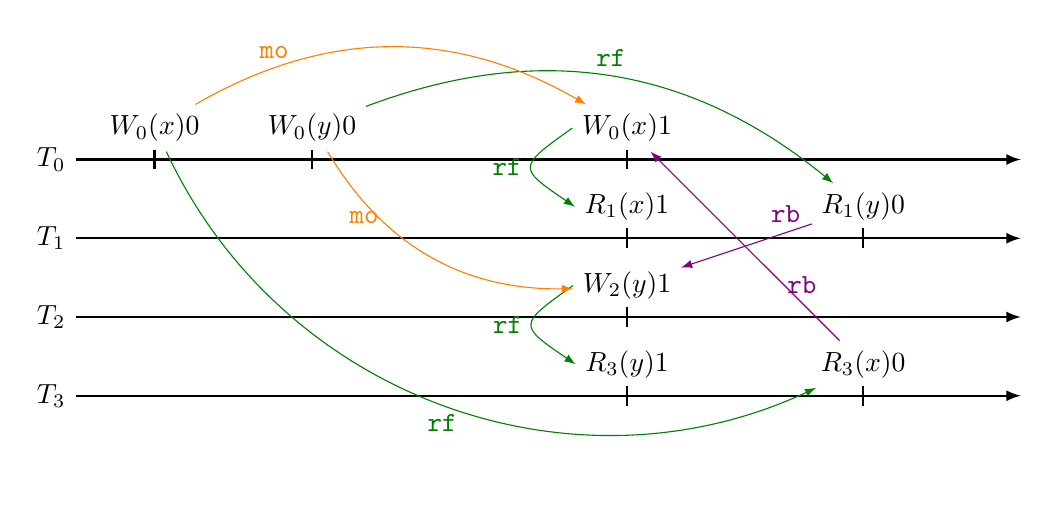
\begin{tikzpicture}[>=latex]
\foreach \i in {0,1,2,3}
  \draw[thick, ->] (0,3-\i) node[left] {$T_\i$} -- +(12,0);

\foreach \i / \j in {1/3, 3/3, 7/3, 7/1, 7/2, 10/2, 7/0, 10/0}
  \draw[thick] (\i,\j) +(0,0.125) -- +(0, -0.125);

\node[above=1mm] at (1,3) (initx) {$W_0(x)0$};
\node[above=1mm] at (3,3) (inity) {$W_0(y)0$};


\node[above=1mm] at (7,3)  (wx) {$W_0(x)1$};
\node[above=1mm] at (7,1)  (wy) {$W_2(y)1$};
\node[above=1mm] at (7,2) (rx1) {$R_1(x)1$};
\node[above=1mm] at (10,2) (ry1) {$R_1(y)0$};
\node[above=1mm] at (7,0) (ry2) {$R_3(y)1$};
\node[above=1mm] at (10,0) (rx2) {$R_3(x)0$};


\draw[Green,->] (wx.west) .. controls +(-0.7, -0.5) .. node[left] {\tt rf} (rx1.west);
\draw[Green,->] (wy.west) .. controls +(-0.7, -0.5) .. node[left] {\tt rf} (ry2.west);

\draw[Green,->] (inity) edge[bend left] node[above] {\tt rf} (ry1);
\draw[Green,->] (initx) edge[bend right=45] node[below] {\tt rf} (rx2);

\draw[orange,->] (initx) edge[bend left] node[above, pos=0.2] {\tt mo} (wx);
\draw[orange,->] (inity) edge[bend right] node[below, pos=0.2] {\tt mo} (wy);

\draw[Purple,->] (rx2) edge node[above, pos=0.2] {\tt rb} (wx);
\draw[Purple,->] (ry1) edge node[above, pos=0.2] {\tt rb} (wy);

\end{tikzpicture}
\end{center}


\section{Alternatives à la \emph{Sequential Consistency}}
\label{sec:release-acquire}

\epigraph{Atomics are like a chainsaw. Everyone can
learn to use one, but don't let yourself get
too comfortable with it.}{Herb Sutter}

Le standard \marque{C11} / \marque{C++11} a introduit des types supportant des
opérations atomiques dans le nouvel en-tête \texttt{stdatomic.h}. Il introduit
aussi un modèle mémoire plus sophistiqué, qui peut offrir un niveau de garantie
variable. Il permet la \emph{sequential consistency}, mais aussi d'autres formes
de garanties qui synchronisent \og moins fort\fg{} et sont donc moins coûteuses.
Ce modèle mémoire a été intégré à \OMP 5.0 et... il est d'une utilisation
complexe. À réserver aux cas désespérés !

Pour cela, on a d'une part des lectures/écritures \og normales\fg
(\emph{relaxed}) qui n'induisent pas de synchronisation entre les
threads. D'autre part, on a des lectures/écritures spéciales :
\begin{itemize}
\item Une \emph{lecture-acquisition} (\emph{read acquire}) d'une variable $x$
  \og prend possession\fg de $x$. Elle s'exécute avant tous les accès à $x$ qui
  suivent dans l'ordre imposé par le programme.

\item Une \emph{écriture-libération} (\emph{store release})d'une variable $x$
  \og rend \fg $x$. Elle s'exécute après tous les accès à $x$ qui précèdent dans
  l'ordre imposé par le programme.
\end{itemize}

Enfin, on peut faire une opération \og\emph{read-modify-write}\fg{} (style
\texttt{pragma omp atomic capture/update}) en mode \emph{release} (la lecture
est \emph{relaxed}, l'écriture est \emph{release}), en mode \emph{acquire}
(l'écriture est \emph{relaxed}) ou bien en mode \emph{release-acquire} (la
lecture et l'écriture sont concernées).


\begin{center}
  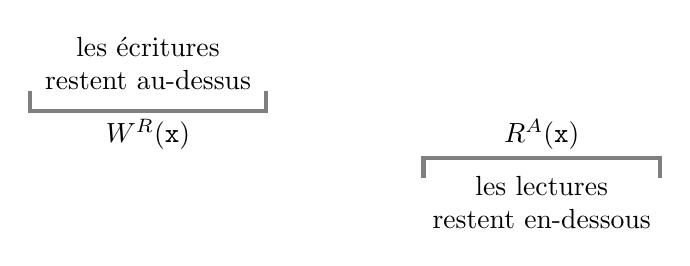
\begin{tikzpicture}
  \node[inner sep=1pt] at (0, 0) (exit0) {$W^{\red R} (\texttt{x})$};  
  \draw[ultra thick, semitransparent] (-1.5, 0.55) -- ++(0, -0.25) -- ++(3, 0) -- ++(0, 0.25);

  \node[align=center, anchor=south] at (0, 0.45) {les écritures \\ restent au-dessus};

  \node[inner sep=1pt] at (5, 0) (enter1) {$R^{\red A} (\texttt{x})$};
  \draw[ultra thick, semitransparent] (3.5, -0.55) -- ++(0, 0.25) -- ++(3, 0) -- ++(0, -0.25);

  \node[align=center, anchor=north] at (5, -0.4) {les lectures \\ restent en-dessous};

  
\end{tikzpicture}
\end{center}


\paragraph{But principal} L'idée générale, c'est que si un thread $T_1$ fait une
lecture-acquisition et \emph{obtient une valeur écrite} par une écriture-libération sur
un autre thread $T_0$, alors cela \emph{synchronise} les deux threads : toutes
les écritures effectuées par $T_0$ auparavant sont alors visibles de $T_1$. Ceci
permet de faire prouvablement fonctionner l'idiome du \emph{message passing}~:
\begin{center}
\begin{tabular}{|c|p{2cm}||p{2cm}|}
  \hline
  État initial : & \multicolumn{2}{c|}{x = 0 ; y = 0} \\
  \hline
  & \tt x = 1;           & \tt a $=^{\red A}$ y; \\
  & \tt y $=^{\red R}$ 1; & \tt b = x; \\
  \hline
  Comportement interdit : & \multicolumn{2}{c|}{a = 1 ; b = 0} \\
  \hline
\end{tabular}
\end{center}

En effet, soit la lecture-acquisition de $y$ obtient l'ancienne valeur et rien
ne se passe (on obtient $a = 0, b = $ undef). Soit la lecture-acquisition de $y$
obtient la valeur issue de l'écriture-libération de $y$, et alors le thread 1
\og voit\fg{} aussi l'écriture sur $x$ qui précède.


Il faut bien comprendre qu'une lecture-acquisition ne va \emph{pas forcément}
obtenir le résultat de l'écriture-libération qui nous intéresse. Mais \emph{si}
c'est le cas, alors une forme de synchronisation entre les mémoires des deux
threads a lieu.


\paragraph{Faiblesse relative} Si toutes les lectures sont \emph{acquire} et
toutes les écritures \emph{release}, qu'obtient-on ? Des garanties assez
faibles, plus faibles que ce qu'offrent naturellement les processeurs TSO en
tout cas. Par exemple, si on reprend l'exemple IRIW :

\begin{center}
\begin{tabular}{|c|p{2cm}||p{2cm}||p{2cm}||p{2cm}|}
  \hline
  État initial : & \multicolumn{4}{c|}{x = 0 ; y = 0} \\
  \hline
  & \tt x $=^{\red R}$ 1; & \tt a $=^{\red A}$ x; & \tt y $=^{\red R}$ 1; & \tt c $=^{\red A}$ y; \\
  & \tt                  & \tt b $=^{\red A}$ y; &                      & \tt d $=^{\red A}$ x; \\
  \hline
  Comportement possible : & \multicolumn{4}{c|}{a = 1 ; b = 0 ; c = 1 ; d = 0} \\
  \hline
\end{tabular}
\end{center}

Pour obtenir le comportement annoncé, il faudrait d'une part que la lecture
$c =^{\red A} y$ se synchronise avec l'écriture $y =^{\red R} 1$, et d'autre
part que $a =^{\red A} x$ se synchronise avec $x =^{\red R} 1$. C'est tout à
fait permis par la sémantique des opérations.

Ce comportement est impossible sur les processeurs TSO, où lorsqu'un thread
effectue une écriture, les autres peuvent ne pas la voir tout de suite, mais ils
voient tous en même temps. En effet, pour avoir $a=1$, il faut que l'écriture de
$x$ soit visible $T_1$, donc par tous les threads. Puisqu'on a $b = 0$, c'est
que l'écriture sur $y$ n'était pas encore visible de $T_1$ au moment où $x=1$
l'était. C'est la même chose du côté de $T_3$ : l'écriture $x=1$ n'était pas
encore visible au moment où $x=1$ l'était. Or ceci est contradictoire : les
écritures effectuées par $T_0$ et $T_2$ doivent être visibles en même temps par
$T_1$ et $T_3$ dans le modèle TSO.

L'idée du modèle \emph{Release-Acquire} est d'offrir un système qui 1) permet
des synchronisations effectives entre threads, mais 2) n'est pas très
contraignant pour pouvoir être efficacement implanté sur les architectures les
plus relâchées.

\subsection{Garanties offertes}

L'idée de la \emph{sequential consistency} est de dire qu'il y a un \emph{ordre}
sur les évènements, compatible avec l'ordre des instructions. Ici aussi, on va
introduire un ordre, mais plus faible.

On dit que $x \hb y$ (\og \emph{happens-before}\fg{}) si l'une de ces trois conditions est réunie :
\begin{itemize}
\item $x \po y$ ($x$ est exécuté avant $y$ par le même thread, \emph{sequenced-before}).
\item $x$ est est écriture-libération, $y$ est une lecture-acquisition et $x \rf y$ (\og $x$ se synchronise avec $y$\fg).
\item Il existe un évènement $z$ tel que $x \hb z$ et $z \hb y$ (la relation est transitive).
\end{itemize}

On définit aussi la relation $\eco = (\rf \cup \mo \cup \rb)^{+}$
(\anglais{extended coherence order}), où le signe $+$ désigne la clôture
transitive. Autrement dit, on a $x \eco y$ si et seulement si l'une des
conditions suivantes est vérifiée :
\begin{enumerate}[$i$)]
\item $x \rf y$
\item $x \mo y$
\item $x \rb y$
\item Il existe $z$ tel que $x \eco z$ et $z \eco y$.
\end{enumerate}

\medskip

Les garanties offerte sur la cohérence de la mémoire sont :
\[
  \hb \text{est irreflexive} \qquad \text{et} \qquad \hb ; \eco  \text{est irreflexive} \tag{\textsc{Coherence}}
\]
Ceci signifie qu'on ne peut pas avoir $x \hb x$ ni $x \hb y \eco x$. Autrement
dit, si $x \hb y$, alors on ne peut pas avoir $y \eco x$. Les seuls
comportements admissibles sont ceux qui ne contredisent pas (\textsc{Coherence})
et (\textsc{Atomicity}).

\subsection{Exemple : Message Passing}

Comme annoncé, utiliser les lectures-acquisition et
les écritures-libération interdit bien le comportement relâché observé pour le
\emph{message passing}. En effet, si on reprend le schéma qui explique ce qui ne
va pas :

\begin{center}
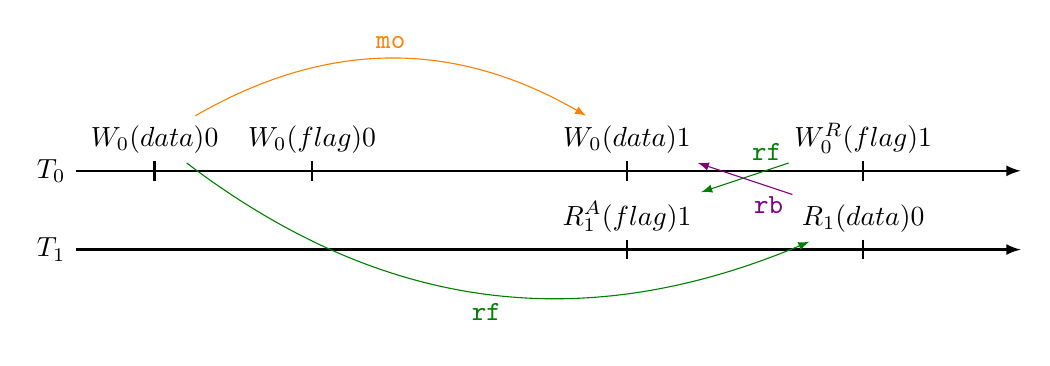
\begin{tikzpicture}[>=latex]
\foreach \i in {0,1}
  \draw[thick, ->] (0,1-\i) node[left] {$T_\i$} -- +(12,0);

\foreach \i / \j in {1/1, 3/1, 7/1, 10/1, 7/0, 10/0}
  \draw[thick] (\i,\j) +(0,0.125) -- +(0, -0.125);

\node[above=1mm] at (1,1) (initx) {$W_0(data)0$};
\node[above=1mm] at (3,1) (inity) {$W_0(flag)0$};


\node[above=1mm] at (7,1)  (wx) {$W_0(data)1$};
\node[above=1mm] at (10,1) (wy) {$W^{\red R}_0(flag)1$};
\node[above=1mm] at (7,0)  (ry) {$R^{\red A}_1(flag)1$};
\node[above=1mm] at (10,0) (rx) {$R_1(data)0$};

\draw[Green,->] (initx) edge[bend right]  node[below] {\tt rf} (rx);
\draw[Green,->] (wy) edge  node[above, near start] {\tt rf} (ry);

\draw[orange,->] (initx) edge[bend left]  node[above] {\tt mo} (wx);

\draw[Purple,->] (rx) edge  node[below, near start] {\tt rb} (wx);
\end{tikzpicture}
\end{center}
L'arête $W^{\red R}_0(flag)1 \rf R^{\red A}_1(flag)1$ donne lieu à une
synchronisation, donc à une arête \emph{happens-before}. On voit qu'on a alors :
\[
  W_0(data)1 \hb W^{\red R}_0(flag)1 \hb R^{\red A}_1(flag)1 \hb R_1(data)0 \rb W_0(data)1
\]
Or ceci est interdit par (\textsc{Coherence}).

\subsection{Exemple : file à deux threads} Considérons une file (FIFO) de capacité finie où
un thread essaye d'enfiler tandis que l'autre essaye de défiler. Si la file est
pleine (resp. vide) alors enfiler (resp. défiler) échoue. La file utilise un
\emph{ring-buffer} (tableau circulaire). 

\begin{minted}{C}
int lo = 0;     // nombre d'éléments défilés
int hi = 0;     // nombre d'éléments enfilés
void * queue[256];

bool enqueue(void *x) 
{
	int l, h;
	#pragma omp atomic acquire read         // synchronise avec la fin de dequeue()
	l = lo;
        h = hi;
	if (hi - lo == 256)
		return false;
	queue[hi & 0xff] = x;
	#pragma omp atomic release write        // synchronise avec le début de dequeue()
	hi = h + 1;
	return true;
}

bool dequeue(void **result) 
{
	int l, h;
	#pragma omp atomic acquire read         // synchronise avec la fin de enqueue()
	h = hi;
        l = lo;
	if (lo == hi)
		return false;
	**result = queue[lo & 0xff];
	#pragma omp atomic release write        // synchronise avec le début de enqueue()
	lo = lo + 1;
	return true;
}
\end{minted}

Avec ces annotations, ou bien \texttt{dequeue} ne \og voit pas\fg{} le dernier
\texttt{enqueue}, ou bien il le voit complètement et vice-versa.

Qu'est-ce qui pourrait mal se passer ? Imaginons que \texttt{enqueue} et
\texttt{dequeue} soient appelés simultanément. Dans le modèle mémoire relâché,
il se pourrait que \texttt{dequeue} voit bien la nouvelle valeur de \texttt{hi}
mais pas le contenu de \mintinline{C}{queue[hi & 0xff]}. Or c'est précisément ce
qui est interdit par les opérations de \emph{release store/read acquire}.

\subsection{Exemple : Peterson Lock (raté)} Cependant, le maniement de ces opérations est un art
\emph{très} délicat. Par exemple, si on reprend le \emph{Peterson lock} :
\begin{myfilet}
\begin{minted}{C}
bool flag[2];
int victim;

void lock() 
{
	int i = omp_get_thread_num();
	int j = 1 - i;
	flag[i] = true;                            // I'm interested
	victim = i;                                // you go first
	while (victim == i && flag[j] == true) {}; // wait
}

void unlock() 
{
	int i = omp_get_thread_num();
	flag[i] = false; // I'm not interested
}
\end{minted}
\end{myfilet}

Et qu'on imagine que \emph{toutes} les écritures sont \emph{release} et que
\emph{toutes} les lectures sont \emph{acquire}, eh bien ça ne suffit pas à
garantir l'exclusion mutuelle. Deux appels à \texttt{lock()} sur deux threads
peuvent obtenir l'accès à la section critique simultanément. En fait, les deux
threads ne sont pas forcés de lire une valeur écrite par l'autre pour accéder à
la section critique : il suffit qu'ils lisent tous les deux les valeurs de
l'état initial. Dans ce cas, aucune lecture ne synchronise avec aucune
écriture. Par exemple, les deux threads peuvent lire la valeur de
\texttt{victim} qu'ils viennent d'écrire, et lire que le \texttt{flag} de
l'autre est \texttt{false}.

En résumé :
\begin{center}
\begin{tabular}{|c|p{2.5cm}||p{2.5cm}|}
  \hline
  État initial : & \multicolumn{2}{c|}{\tt f0 = f1 = 0, v=0} \\
  \hline
                 & \tt f0 = 1; & \tt f1 = 1; \\
                 & \tt v = 0;  & \tt v = 1; \\
                 & \tt a = v;  & \tt c = v; \\
                 & \tt b = f1; & \tt d = f0; \\

  \hline
  Comportement relâché : & \multicolumn{2}{c|}{a = 0, b = 0, c = 1, d = 0} \\
  \hline
\end{tabular}
\end{center}

Et ça peut par exemple se passer comme ceci :
\begin{center}
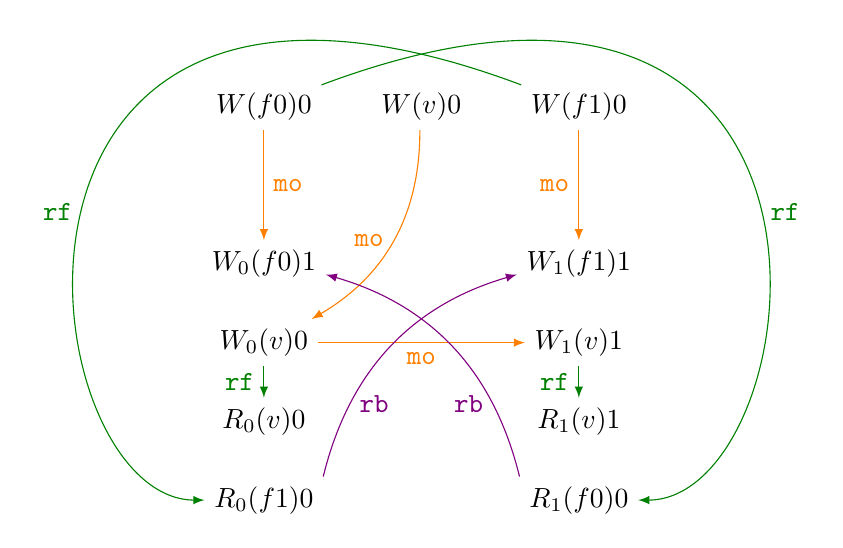
\begin{tikzpicture}[>=latex]
  \path[red, use as bounding box] (-5, 3) rectangle (5, -3.25);
  \node at (-2, 2) (initf0) {$W(f0)0$};
  \node at (0, 2)  (initv) {$W(v)0$};
  \node at (2, 2)  (initf1) {$W(f1)0$};

  
  \node at (-2,0)   (W0f) {$W_0(f0)1$};
  \node at (-2,-1 ) (W0v) {$W_0(v)0$};
  \node at (-2, -2) (R0v) {$R_0(v)0$};
  \node at (-2, -3) (R0f) {$R_0(f1)0$};

  \node at (2,0)   (W1f) {$W_1(f1)1$};
  \node at (2,-1 ) (W1v) {$W_1(v)1$};
  \node at (2, -2) (R1v) {$R_1(v)1$};
  \node at (2, -3) (R1f) {$R_1(f0)0$};

  
\draw[Green,->] (initf0) .. controls (6, 5) and (5, -3) ..  node[right] {\tt rf}  (R1f);
\draw[Green,->] (initf1) .. controls (-6, 5) and (-5, -3) .. node[left] {\tt rf} (R0f);
\draw[Green,->] (W0v) edge node[left] {\tt rf} (R0v);
\draw[Green,->] (W1v) edge node[left] {\tt rf} (R1v);

\draw[orange,->] (initf0) edge[] node[right] {\tt mo} (W0f);
\draw[orange,->] (initf1) edge[] node[left] {\tt mo} (W1f);
\draw[orange,->] (initv)  edge[bend left] node[left] {\tt mo} (W0v);
\draw[orange,->] (W0v)  edge node[below] {\tt mo} (W1v);

\draw[Purple,->] (R1f.north west) to[bend right]  node[near start,left] {\tt rb} (W0f);
\draw[Purple,->] (R0f.north east) to[bend left]  node[near start,right] {\tt rb} (W1f);

 % \draw[gray,->] (R0) edge[out=180, in=180]  node[left] {\tt rmw} (W0.west);
 % \draw[gray,->] (R1) edge[out=0, in=0]  node[right] {\tt rmw} (W1.east);
\end{tikzpicture}
\end{center}

Ceci n'est pas contradictoire avec (\textsc{Coherence}).

\subsection{Exemple : Peterson Lock (réussi)} Pour que ça puisse marcher, il faut forcer
les deux threads à se synchroniser. Quelle variable doit forcément être accédée
par les deux threads? \texttt{victim}. Pour les synchroniser, on peut utiliser
une opération \emph{read-modify-write} atomique.  Ici, on effectue aussi une
\emph{lecture-acquisition} de \texttt{victim} avant d'en faire une
écriture-libération.

\begin{myfilet}
\begin{minted}{C}
volatile bool flag[2];
volatile int victim;

void lock() 
{
	int i = omp_get_thread_num();
	int j = 1 - i;
        flag[i] = true;                            // I'm interested
        int foo;
        #pragma omp atomic rel_acq capture
        { foo = victim; victim = i; }              // you go first
	victim = i;                                
	while (true) {                             // wait while I'm the victim 
                int v, f;                          // and the other is interested
                v = victim;
                #pragma omp atomic acquire read
                f = flag[1 - i];
                if (v != i || f == false)
                        break
        }
}

void unlock() 
{
	int i = omp_get_thread_num();
        #pragma omp atomic release write
        flag[i] = false;                           // I'm not interested
}
\end{minted}
\end{myfilet}

L'accès \emph{release-acquire} à \texttt{victim} sert à synchroniser deux appels
concurrents à \texttt{lock()}. L'écriture-libération de \texttt{flag[i]} dans
\texttt{unlock()} à vocation à se synchroniser avec la lecture-acquisition de
\texttt{flag[1-i]} dans \texttt{lock()}. Ceci garantit que toutes les écritures
qui ont eu lieu dans la section critique précédente sont bien \og visibles\fg{}
dans la section critique suivante (car elles \emph{happens before}).
\begin{center}
\begin{tikzpicture}
  \node at (0, 3) (lock0) {\texttt{lock()}};
  \node[inner sep=1pt] at (0, 0.5) (exit0) {$W^{\red R}_0 (\texttt{flag[0]}) 0$};  

  \draw[ultra thick, semitransparent] (exit0.north west) ++(-0.25, 0.30) -- ++(0, -0.25) -- ++(3, 0) -- ++(0, 0.25);

  \draw (lock0) edge[dashed,->] node[left] (CS0) {Section critique} ($ (exit0.north) + (0, 0.15) $);

  \draw[decorate, decoration=brace] (1, 2.75) -- (1, 1) ;

  
  \node at (0, 0) {\texttt{unlock()}};

  \draw[dotted] (2.5, 3.5) -- +(0, -8);
  
  \node at (5, -1) {\texttt{lock()}};
  \node[inner sep=1pt] at (5, -1.5) (enter1) {$R^{\red A}_1 (\texttt{flag[0]})0$};
  \draw[ultra thick, semitransparent] (enter1.south west) ++(-0.25, -0.30) -- ++(0, 0.25) -- ++(3, 0) -- ++(0, -0.25);

  \node at (5, -4) (exit1) {};
  \draw (enter1) edge[dashed,->] node[right] (CS1) {Section critique} (exit1);

  \draw[blue, ->] (exit0.south east) to node[above] {\tt hb} (enter1.north west);

  \draw[red, ->] (1.25, 1.75) to[bend left,in=120] node[above,sloped] {toutes les écritures sont visibles}  (CS1.north east);  
\end{tikzpicture}
\end{center}

Essayons de montrer que ce code garantit l'exclusion mutuelle. Le schéma général de la démonstration est le suivant :
\begin{enumerate}
\item Supposons que les deux threads entrent simultanément dans la section critique.
\item \emph{read-modify-write} : un et un seul thread (disons $T_1$) lit la valeur de \texttt{victim} écrite par l'autre ($T_0$, donc).
\item Forcément, $T_1$ écrit \texttt{victim = 1} après que $T_0$ ait fait \texttt{victim = 0}.
\item Dans ces conditions, $T_1$ ne peut pas entrer dans la section critique avec \texttt{victim == 0}.
\item $T_1$ lit donc \texttt{victim == 1}, et à cause de la synchronisation, $T_1$ ne peut pas lire \texttt{flag[0] == false}.
\item Par conséquent, $T_1$ ne peut pas sortir de la boucle \texttt{while}. Contradiction !
\end{enumerate}

\subsubsection{\emph{read-modify-write} : $T_1$ lit la valeur de \texttt{victim} écrite par $T_0$.}

% Le thread 0 peut sortir de la boucle \texttt{while} de deux manières possibles :
% soit il a \og vu\fg{} \texttt{victim == 1}, soit il a vu \texttt{victim == 0} et
% \texttt{flag[1] == false}. De manière symétrique, le thread 1 peut sortir de la
% boucle s'il a \og vu\fg{} \texttt{victim == 0}, soit il a vu \texttt{victim ==
%   1} et \texttt{flag[0] == false}. Il y a donc $2 \times 2$ comportements
% interdits à examiner.

Dans une exécution du code où les deux threads pénètrent simultanément dans la
section critique, on a :

\begin{center}
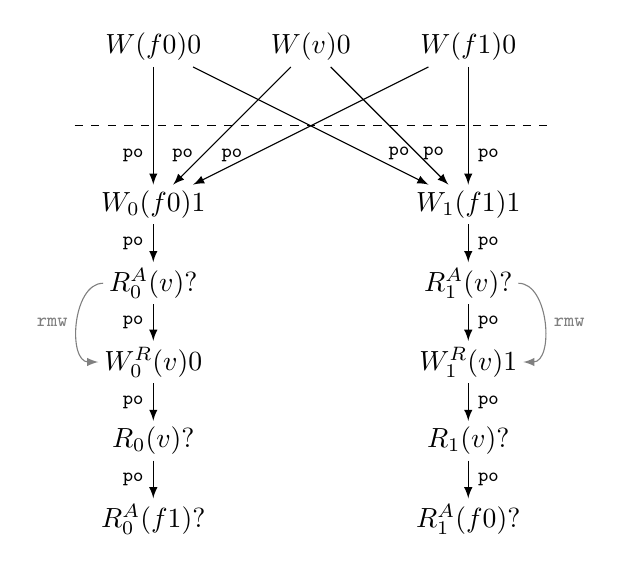
\begin{tikzpicture}[>=latex,every node/.style={inner sep=2pt}]
  \node at (-2, 2) (initf0) {$W(f0)0$};
  \node at (0, 2)  (initv) {$W(v)0$};
  \node at (2, 2)  (initf1) {$W(f1)0$};

  \draw[dashed] (-3, 1) -- (3, 1);
  
  \node at (-2, 0)   (W0f) {$W_0(f0)1$};
  \node at (-2, -1) (R0va) {$R^{\red A}_0(v)?$};
  \node at (-2, -2) (W0v) {$W^{\red R}_0(v)0$};
  \node at (-2, -3) (R0v) {$R_0(v)?$};
  \node at (-2, -4) (R0f) {$R^{\red A}_0(f1)?$};

  \node at (2, 0)  (W1f) {$W_1(f1)1$};
  \node at (2, -1) (R1va) {$R^{\red A}_1(v)?$};
  \node at (2, -2) (W1v) {$W^{\red R}_1(v)1$};
  \node at (2, -3) (R1v) {$R_1(v)?$};
  \node at (2, -4) (R1f) {$R^{\red A}_1(f0)?$};
  
  \begin{scope}[every node/.style={font={\ttfamily\scriptsize}}]
    \draw[->] (initf0) edge node[near end,left] {po} (W0f) edge node[very near end,above] {po} (W1f);
    \draw[->] (initf1) edge node[near end,left] {po} (W0f) edge node[near end,right] {po} (W1f);
    \draw[->] (initv) edge node[near end,left] {po} (W0f) edge node[very near end,above] {po} (W1f);

    \draw[gray,->] (R0va) edge[out=180, in=180]  node[left] {\tt rmw} (W0v.west);
    \draw[gray,->] (R1va) edge[out=0, in=0]  node[right] {\tt rmw} (W1v.east);

      
    \draw[->] (W0f) edge node[left] {po} (R0va);
  \draw[->] (R0va) edge node[left] {po} (W0v);
  \draw[->] (W0v) edge node[left] {po} (R0v);
  \draw[->] (R0v) edge node[left] {po} (R0f);

  \draw[->] (W1f) edge node[right] {po} (R1va);
  \draw[->] (R1va) edge node[right] {po} (W1v);
  \draw[->] (W1v) edge node[right] {po} (R1v);
  \draw[->] (R1v) edge node[right] {po} (R1f);
\end{scope}
\end{tikzpicture}
\end{center}

La première lecture de \texttt{victim} que fait chaque thread doit provenir
d'une certaine écriture. Et il n'y a que deux solutions : soit elle provient de
la valeur initiale, soit elle provient de la valeur écrite par l'autre
thread. Il y a donc trois cas (le scénario 2 admet un cas symétrique où $T_0$
lit la valeur écrite par $T_1$) :

\begin{center}
  \begin{tabular}{|c|c|c|}
    \hline
    Scénario 1 & Scénario 2 & Scénario 3 \\
    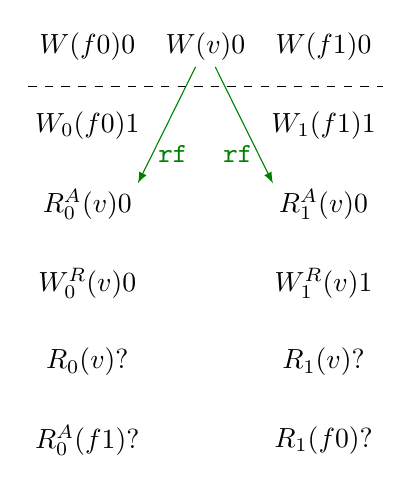
\begin{tikzpicture}[>=latex,xscale=0.75,every node/.style={inner sep=2pt}]
      \node at (-2, 1) (initf0) {$W(f0)0$};
      \node at (0, 1)  (initv) {$W(v)0$};
      \node at (2, 1)  (initf1) {$W(f1)0$};
      
      \draw[dashed] (-3, 0.5) -- (3, 0.5);
      
      \node at (-2, 0)   (W0f) {$W_0(f0)1$};
      \node at (-2, -1) (R0va) {$R^{\red A}_0(v)0$};
      \node at (-2, -2) (W0v) {$W^{\red R}_0(v)0$};
      \node at (-2, -3) (R0v) {$R_0(v)?$};
      \node at (-2, -4) (R0f) {$R^{\red A}_0(f1)?$};
      
      \node at (2, 0)  (W1f) {$W_1(f1)1$};
      \node at (2, -1) (R1va) {$R^{\red A}_1(v)0$};
      \node at (2, -2) (W1v) {$W^{\red R}_1(v)1$};
      \node at (2, -3) (R1v) {$R_1(v)?$};
      \node at (2, -4) (R1f) {$R_1(f0)?$};
      
  \draw[Green,->] (initv) edge[] node[right, near end] {\tt rf} (R0va.north east);
  \draw[Green,->] (initv) edge[] node[left, near end] {\tt rf} (R1va.north west);  
\end{tikzpicture}
    &      
    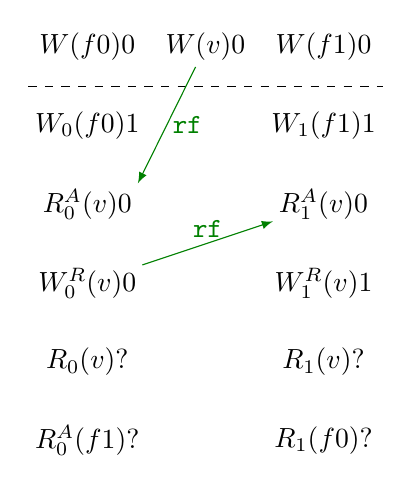
\begin{tikzpicture}[>=latex,xscale=0.75,every node/.style={inner sep=2pt}]
      \node at (-2, 1) (initf0) {$W(f0)0$};
      \node at (0, 1)  (initv) {$W(v)0$};
      \node at (2, 1)  (initf1) {$W(f1)0$};
      
      \draw[dashed] (-3, 0.5) -- (3, 0.5);
      
      \node at (-2, 0)   (W0f) {$W_0(f0)1$};
      \node at (-2, -1) (R0va) {$R^{\red A}_0(v)0$};
      \node at (-2, -2) (W0v) {$W^{\red R}_0(v)0$};
      \node at (-2, -3) (R0v) {$R_0(v)?$};
      \node at (-2, -4) (R0f) {$R^{\red A}_0(f1)?$};
      
      \node at (2, 0)  (W1f) {$W_1(f1)1$};
      \node at (2, -1) (R1va) {$R^{\red A}_1(v)0$};
      \node at (2, -2) (W1v) {$W^{\red R}_1(v)1$};
      \node at (2, -3) (R1v) {$R_1(v)?$};
      \node at (2, -4) (R1f) {$R_1(f0)?$};
      
  \draw[Green,->] (W0v) edge[] node[above] {\tt rf} (R1va);
  \draw[Green,->] (initv) edge[] node[right] {\tt rf} (R0va.north east);  
\end{tikzpicture}
                            &
                                  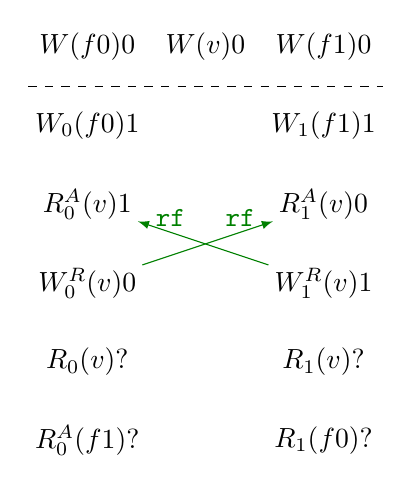
\begin{tikzpicture}[>=latex,xscale=0.75,every node/.style={inner sep=2pt}]
      \node at (-2, 1) (initf0) {$W(f0)0$};
      \node at (0, 1)  (initv) {$W(v)0$};
      \node at (2, 1)  (initf1) {$W(f1)0$};
      
      \draw[dashed] (-3, 0.5) -- (3, 0.5);
      
      \node at (-2, 0)   (W0f) {$W_0(f0)1$};
      \node at (-2, -1) (R0va) {$R^{\red A}_0(v)1$};
      \node at (-2, -2) (W0v) {$W^{\red R}_0(v)0$};
      \node at (-2, -3) (R0v) {$R_0(v)?$};
      \node at (-2, -4) (R0f) {$R^{\red A}_0(f1)?$};
      
      \node at (2, 0)  (W1f) {$W_1(f1)1$};
      \node at (2, -1) (R1va) {$R^{\red A}_1(v)0$};
      \node at (2, -2) (W1v) {$W^{\red R}_1(v)1$};
      \node at (2, -3) (R1v) {$R_1(v)?$};
      \node at (2, -4) (R1f) {$R_1(f0)?$};
      
  \draw[Green,->] (W1v) edge[] node[near end, above] {\tt rf} (R0va);
  \draw[Green,->] (W0v) edge[] node[near end, above] {\tt rf} (R1va);  
\end{tikzpicture}
    \\
    \hline
  \end{tabular}
\end{center}

Le plus facile à éliminer est le scénario 3. En effet, on a des
lecture-acquisition qui obtiennent le résultat d'écritures-libérations. Il y a
donc synchronisation et des arêtes \emph{happens-before}. On a donc un cycle :
\[
  R^{\red A}_0(v)1 \hb W^{\red R}_0(v)0 \hb R^{\red A}_1(v)?0 \hb W^{\red R}_1(v)? \hb R^{\red A}_0(v)1
\]
qui est interdit par (\textsc{Coherence}).


Le scénario 1 exhibe un défaut d'atomicité. Les deux threads écrivent
\texttt{victim}, donc l'un des deux va écrire en dernier ($\mo$ est un ordre
total sur une variable donnée). Supposons, sans perte de généralité car la
situation est symétrique, que le thread zéro écrive \texttt{victim} en dernier. Alors on a :

\begin{center}
    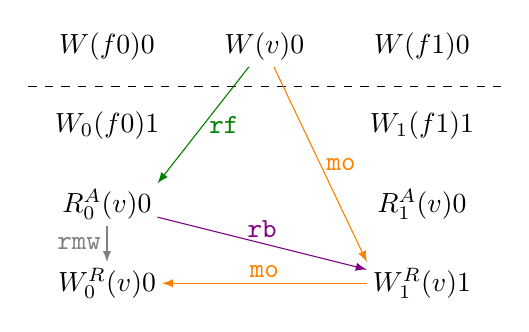
\begin{tikzpicture}[>=latex,every node/.style={inner sep=2pt}]
  \node at (-2, 1) (initf0) {$W(f0)0$};
  \node at (0, 1)  (initv) {$W(v)0$};
  \node at (2, 1)  (initf1) {$W(f1)0$};

  \draw[dashed] (-3, 0.5) -- (3, 0.5);
  
  \node at (-2, 0)   (W0f) {$W_0(f0)1$};
  \node at (-2, -1) (R0va) {$R^{\red A}_0(v)0$};
  \node at (-2, -2) (W0v) {$W^{\red R}_0(v)0$};

  \node at (2, 0)  (W1f) {$W_1(f1)1$};
  \node at (2, -1) (R1va) {$R^{\red A}_1(v)0$};
  \node at (2, -2) (W1v) {$W^{\red R}_1(v)1$};

  \draw[Green,->] (initv) edge[] node[right] {\tt rf} (R0va.north east);

  \draw[orange,->] (initv) edge[] node[right] {\tt mo} (W1v.north west);
  \draw[orange,->] (W1v) edge node[above] {\tt mo} (W0v);

  \draw[gray,->] (R0va) edgenode[left] {\tt rmw} (W0v);
  \draw[Purple,->] (R0va) edge node[above] {\tt rb} (W1v);
\end{tikzpicture}
\end{center}

Et donc on voit que ceci contredit (\textsc{Atomicity}), car on a à la fois
$R_0(v)0 \rmw W_0(v)0$ et $R_0(v)0 \rb W_1(v)1 \mo W_0(v)0$.

Reste donc seulement le scénario 2. Dans ce cas, la lecture-acquisition de
\texttt{victim} par $T_1$ se synchronise avec l'écriture-libération par
$T_0$.

\subsubsection{$T_1$ écrit \texttt{victim} après $T_0$}

%Commençons par remarquer qu'aucun des threads ne peut lire la valeur initiale de
%\texttt{victim} après avoir écrit lui-même dessus. 

Comme $T_1$ lit la valeur de \texttt{victim} écrite par $T_0$, on peut affirmer
que $T_1$ il écrit sa propre valeur de \texttt{victim} \emph{après}. On a donc
$W^{\red R}_0(v)0 \mo W^{\red R}_1(v)1$. En effet, supposons que ce soit le
contraire :
\begin{center}
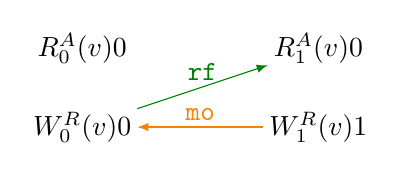
\begin{tikzpicture}[>=latex,xscale=0.75,every node/.style={inner sep=2pt}]
      \node at (-2, -1) (R0va) {$R^{\red A}_0(v)0$};
      \node at (-2, -2) (W0v) {$W^{\red R}_0(v)0$};
      
      \node at (2, -1) (R1va) {$R^{\red A}_1(v)0$};
      \node at (2, -2) (W1v) {$W^{\red R}_1(v)1$};
      
  \draw[Green,->] (W0v) edge[] node[above] {\tt rf} (R1va);
  \draw[orange,->] (W1v) edge[] node[above] {\tt mo} (W0v);  
\end{tikzpicture}
\end{center}
On voit que ceci est contradictoire avec (\textsc{Coherence}), puisqu'on a :
\[
  W^{\red R}_0(v)0 \hb R^{\red A}_1(v)0 \hb W^{\red R}_1(v)1 \quad \text{suivi de} \quad W^{\red R}_1(v)1  \mo W^{\red R}_0(v)0.
\]

\subsubsection{$T_1$ ne peut pas entrer dans la section critique avec \texttt{victim == 0}}

Montrons ensuite que $T_1$ ne peut pas entrer dans la section critique en ayant
lu \texttt{victim == 0}. En effet, si c'était le cas on aurait :
\begin{center}
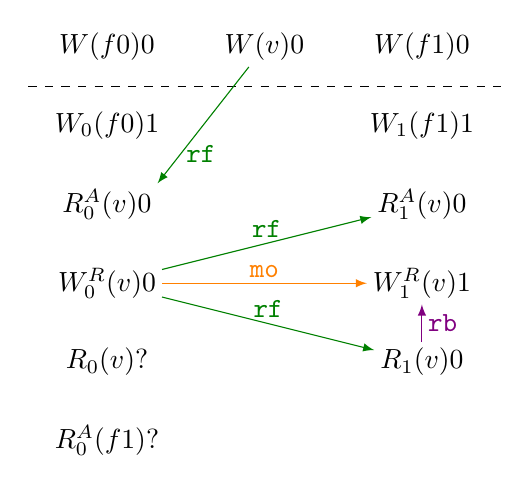
\begin{tikzpicture}[>=latex,every node/.style={inner sep=2pt}]
  \node at (-2, 1) (initf0) {$W(f0)0$};
  \node at (0, 1)  (initv) {$W(v)0$};
  \node at (2, 1)  (initf1) {$W(f1)0$};

  \draw[dashed] (-3, 0.5) -- (3, 0.5);
  
  \node at (-2, 0)   (W0f) {$W_0(f0)1$};
  \node at (-2, -1) (R0va) {$R^{\red A}_0(v)0$};
  \node at (-2, -2) (W0v) {$W^{\red R}_0(v)0$};
  \node at (-2, -3) (R0v) {$R_0(v)?$};
  \node at (-2, -4) (R0f) {$R^{\red A}_0(f1)?$};

  \node at (2, 0)  (W1f) {$W_1(f1)1$};
  \node at (2, -1) (R1va) {$R^{\red A}_1(v)0$};
  \node at (2, -2) (W1v) {$W^{\red R}_1(v)1$};
  \node at (2, -3) (R1v) {$R_1(v)0$};

  \draw[Green,->] (initv) edge[] node[right, near end] {\tt rf} (R0va.north east);
  \draw[Green,->] (W0v) edge[] node[above] {\tt rf} (R1va);  
%  \draw[Green,->] (W0v) edge[] node[left] {\tt rf} (R0v);
  \draw[Green,->] (W0v) edge node[above] {\tt rf} (R1v);
  \draw[orange,->] (W0v) edge[] node[above] {\tt mo} (W1v);  
  \draw[Purple,->] (R1v) edge node[right] {\tt rb} (W1v);
\end{tikzpicture}
\end{center}
Et ceci contredit encore (\textsc{Coherence}), puisqu'on a :
\[
  W^{\red R}_1(v)1 \hb R_1(v)0 \quad \text{et en même temps} \quad R_1(v)0 \rb W^{\red R}_1(v)1.
\]

\subsubsection{$T_1$ ne peut pas lire \texttt{flag[0] == false}}

Le thread $T_1$ a donc forcément perçu \texttt{victim == 1}. Pour entrer dans la
section critique, il faut qu'il lise \texttt{flag[0] == true}, et on va voir que
ceci est impossible. En effet, pour que cela ait lieu, il faudrait que :
\begin{center}
  \begin{tikzpicture}[>=latex,every node/.style={inner sep=2pt}]
    \path[use as bounding box] (-5.25, 1.5) rectangle (3, -5);
    \node at (-2, 1) (initf0) {$W(f0)0$};
  \node at (0, 1)  (initv) {$W(v)0$};
  \node at (2, 1)  (initf1) {$W(f1)0$};

  \draw[dashed] (-3, 0.5) -- (3, 0.5);
  
  \node at (-2, 0)   (W0f) {$W_0(f0)1$};
  \node at (-2, -1) (R0va) {$R^{\red A}_0(v)0$};
  \node at (-2, -2) (W0v) {$W^{\red R}_0(v)0$};
  \node at (-2, -3) (R0v) {$R_0(v)?$};
  \node at (-2, -4) (R0f) {$R^{\red A}_0(f1)?$};

  \node at (2, 0)  (W1f) {$W_1(f1)1$};
  \node at (2, -1) (R1va) {$R^{\red A}_1(v)0$};
  \node at (2, -2) (W1v) {$W^{\red R}_1(v)1$};
  \node at (2, -3) (R1v) {$R_1(v)1$};
  \node at (2, -4) (R0f) {$R^{\red A}_1(f0)0$};

  \draw[orange,->] (initf0) edge node[very near end,left] {\tt mo} (W0f);
  \draw[Green,->] (initv) edge[] node[right, near end] {\tt rf} (R0va.north east);
  \draw[Green,->] (W0v) edge[] node[above] {\tt rf} (R1va);  

  \draw[Green,->] (W1v) edge node[right] {\tt rf} (R1v);
  \draw[orange,->] (W0v) edge[] node[above] {\tt mo} (W1v);
  \draw[Green,->] (W0v) edge[] node[left] {\tt rf} (R0v);

  \draw[Green,->] (initf0) .. controls (-6, 0) and (-6, -7) .. node[left] {\tt rf} (R1f.south);
  \draw[Purple,->] (R1f.south west)  .. controls  (-5, -6) and (-5, -0.5) .. node[right] {\tt rb} (W0f);
\end{tikzpicture}
\end{center}

On voit que (\textsc{Coherence}) est mise en défaut encore une fois, puisqu'on a
:
\[
W_0(f0)1 \hb R^{\red A}_1(v)0 \hb W^{\red R}_0(v)0 \hb R^{\red A}_1(v)0 \hb W_1(v)1 \hb R_1(v)_1 \hb R_1(f0)0 \quad \text{puis} \quad  R^{\red A}_1(f0)0 \rb W_0(f0)1.
\]
Ceci conclut la preuve.



%Verifying C11 Programs Operationally de Simon Doherty et al. (peterson en RA)


% \section{Barrières mémoire (\anglais{Memory Fences})}

% Pour permettre que l'ordre puisse régner dans le chaos des modèles mémoires
% relâchés, les processeurs possèdent des instructions de synchronisation.

% Il y a quatre type de barrière mémoire : LoadLoad, LoadStore, StoreLoad et
% StoreStore. Les barrières empêchent le réordonnancement d'opérations.

% La barrière LoadLoad garantit que les lectures antérieures s'exécutent avant les
% lectures postérieures. Ceci empêche des lectures antérieures d'obtenir des
% valeurs \og plus fraîches\fg{} que des lectures postérieures.

% La barrière StoreStore garantit que les écritures antérieures s'exécutent avant
% les écritures postérieures.

% La barrière LoadStore garantit que les lectures antérieures s'exécutent avant
% les écritures postérieures (le processeur ne s'autorisera pas à permuter
% arbitrairement ces opérations).

% Enfin, La barrière StoreLoad garantit que les lectures antérieures s'exécutent avant
% les écritures postérieures.




% Par exemple, les processeurs \marque{x86-64} en ont trois :

% \begin{description}
  
% \item[\texttt{mfence}] (\anglais{Full Memory Fence}) Garantit que tous les accès
%   à la mémoire qui précèdent l'instruction \texttt{mfence} dans l'ordre imposé
%   par le programme sont terminées (et globalement visibles) avant qu'un accès
%   mémoire qui suit \texttt{mfence} (dans l'ordre imposé par le programme) ne
%   puisse avoir lieu. Latence $\approx 35-40$ cycles.

% \item[\texttt{lfence}] (\anglais{Load-Load Fence}) Garantit que toutes les
%   lectures de la mémoire qui précèdent \texttt{lfence} sont terminées avant
%   qu'une lecture qui suit \texttt{lfence} ne puisse avoir lieu. En particulier,
%   une lecture avant ne peut pas renvoyer une valeur \og plus ancienne\fg qu'une
%   lecture après. Latence $\approx 4-6$ cycles.

% \item[\texttt{sfence}] (\anglais{Store-Store Fence}) Garantit que toutes les
%   écritures dans la mémoire qui précèdent \texttt{sfence} sont terminées (et
%   globalement visibles par les autres threads) avant qu'une écriture qui suit
%   \texttt{sfence} ne puisse avoir lieu. Latence $\approx 5-7$ cycles.
% \end{description}

% \medskip

% Les autres architectures ont des instructions comparables, avec encore plus de
% variantes : il y a des versions \anglais{Load-Store}, \anglais{Store-Load}, les
% processeurs \marque{POWER} ont aussi une \og Store-Load Light fence\fg qui
% garantit que les écritures qui précèdent sont bien visibles lorsque les lectures
% suivantes \emph{du thread courant} auront lieu, mais les écritures antérieures
% peuvent se propager aux autres threads plus tard...

% Insérer des \anglais{Full Memory Fences} entre tous les accès mémoire restaure
% la \anglais{sequential consistency}, mais ralentit considérablement
% l'exécution. Savoir où il faut en mettre exactement, et de laquelle on peut se
% contenter (la lente, complète, ou les rapides, partielles ?) est un art
% délicat. Mieux vaut laisser le compilateur ou \OMP se débrouiller
% (cf. section~\ref{sec:release-acquire}).



\begin{quote}
  A tourist takes a taxi in a foreign town. The taxi driver speeds through a red
  light. The tourist, frightened, asks ``What are you are doing?'' The driver
  answers: ``Do not worry, I am an expert.'' He speeds through more red lights,
  and the tourist, on the verge of hysteria, complains again, more urgently. The
  driver replies, ``Relax, relax, you are in the hands of an expert.'' Suddenly,
  the light turns green, the driver slams on the brakes, and the taxi skids to a
  halt. The tourist picks himself off the floor of the taxi and asks ``For
  crying out loud, why stop now that the light is finally green?'' The driver
  answers ``Too dangerous, could be another expert crossing.''
\end{quote}

\section*{Notes}

La \emph{sequential consistency} a été formalisée pour la première fois
dans~\cite{Lamport79} en 1979. Le theorème~\ref{thm:sc_slow} provient
de~\cite{Lipton1988PramAS}, qui définit le modèle PRAM. Le Peterson lock a été
décrit en 1981 dans~\cite{Peterson81}. La totalité des mini-exemples sont des
\emph{litmus tests} tirés de~\cite{Maranget12}. La formalisation de la
sequential consistency est tirée d'un cours du MPRI de Luc Maranget. La
formalisation des garanties offertes par les opérations \emph{acquire-release}
est une simplification du modèle RC11 présenté dans~\cite{LahavVKHD17} --- ça
date de 2017. Des idées viennent aussi de~\cite{LahavGV16} (notamment la
remarque que RA est plus faible que TSO et une jolie implémentation de RCU).

Merci à Luc Maranget qui a répondu à de nombreuses questions. Jeff Preshing a un
beau site web qui essaye d'expliquer certains de ces concepts.

\part{Aspects architecturaux}









ajouter blocking qui améliore la localité temporelle. Modèle 3C, stack distance. définir localité temporelle et spatiale.


\chapter{Le \og \emph{Memory Wall}\fg}
\label{chap:memory}

L'expression \og \anglais{Memory Wall}\fg a été utilisée pour la première fois
au milieu des années 1990 dans un article de recherche nommé : ``\emph{Hitting
  the Memory Wall: Implications of the Obvious}''~\cite{wulf1995hitting}. Il
commence par ces quelques mots :
\begin{quote}
  This brief note points out something obvious --- something the authors
  ``knew'' without really understanding. With apologies to those who did
  understand, we offer it to those others who, like us, missed the point.
\end{quote}

L'expression \anglais{Memory Wall}, qui a eu un grand succès, mets un nom sur un
phénomène simple : la puissance de calcul des CPUs (typiquement le nombre
d'opérations flottantes par seconde) augmente plus vite que le débit de la
mémoire (le nombre de flottants qui peuvent être transférés de/vers la mémoire
par seconde). La figure~\ref{fig:memwall_bw} montre la tendance depuis les
années 1990.

\begin{figure}
  \includegraphics[width=\textwidth]{calpin_wall_bw.png}
  \caption{Le \og \emph{Memory Wall}\fg, partie 1. La courbe montre le nombre
    d'opérations sur des flottants que les processeurs ont le temps d'effectuer
    à chaque fois qu'un flottant peut être lu depuis la mémoire : cette quantité
    ne fait qu'augmenter. Autrement dit : la puissance de calcul augmente plus
    vite que le \emph{débit} de la mémoire (image: John
    McCalpin). \label{fig:memwall_bw}}
\end{figure}

\begin{figure}
  \includegraphics[width=\textwidth]{calpin_wall_latence.png}
  \caption{Le \og \emph{Memory Wall}\fg, partie 2. La puissance de calcul
    augmente \emph{encore plus vite} que la \emph{latence} de la mémoire. Et
    encore, il s'agit de la latence \og au repos\fg (\anglais{idle latency}), et
    pas de la latence \og en pleine charge\fg (\anglais{loaded latency}), qui
    est typiquement $3\times$ ou $4\times$ plus importante...  (image: John
    McCalpin). \label{fig:memwall_lat}}
\end{figure}


En fait, l'écart augmente exponentiellement au cours du temps. Et l'augmentation
du nombre de coeurs ne fait qu'aggraver le problème, car les coeurs se trouvent
en concurrence les uns avec les autres pour accéder à la mémoire. Evidemment,
ceci pose un problème : les CPUs modernes risquent de passer une fraction sans
cesse plus grande de leur temps à \emph{attendre} des données, plutôt qu'à faire
des calculs utiles.

Ceci est encore aggravé par le fait que l'écart entre le nombre de FLOPS
réalisable par les processeurs et la \emph{latence} des accès mémoire augmente
encore plus vite que l'écart avec le \emph{débit} de la mémoire
(cf. fig.~\ref{fig:memwall_lat}).

Du coup, on est amené à distinguer des algorithmes qui sont
\anglais{compute-bound} (les CPUs ne peuvent pas faire de FLOPs assez vite) de
ceux qui sont \anglais{memory-bound} (les données n'arrivent pas assez vite de
la mémoire pour alimenter les CPUs). Dans ces derniers, on pourrait chercher à
distinguer ceux qui sont limités par le débit de la mémoire d'un côté, ou par sa
latence de l'autre.

\section{Le Matériel sous-jascent}

Dans les ordinateurs contemporains, la mémoire dite \og vive\fg
(\anglais{Random-Access memory}, RAM) est caractérisée par le fait que ce n'est
pas un stockage pérenne (quand on coupe le courant, les données sont perdues),
que les opérations de lecture-écriture sont rapides et ne nécessitent pas de \og
préparation\fg coûteuse (comme le fait de pré-positionner une tête de lecture
sur un disque, etc.)

Si on cherche \og 16Go RAM\fg dans le moteur de recheche du site
\url{amazon.fr}, on a le droit à 50\ 000+ suggestions, parmi lesquelles se
trouvent les cinq produits suivants, tous de la même marque:
\begin{itemize}
\item Produit $x$ 16Go (DDR4, 2666 MT/s, PC4-21300, Dual Rank $\times 4$, ECC, Registered, DIMM, 288-Pin)
\item Produit $y$ 16Go (DDR4, 2666 MT/s, PC4-21300, Dual Rank $\times 8$, Unbuffered, DIMM, 288-Pin)
\item Produit $z$ 16Go (DDR4, 2666 MT/s, PC4-21300, Single Rank $\times 4$, ECC, Registered, DIMM, 288-Pin)
\item Produit $u$ 16Go (DDR4, 2666 MT/s, PC4-21300, Dual Rank $\times 8$, ECC, Unbuffered, DIMM, 288-Pin)
\item Produit $v$ 16Go (DDR4, 2666 MT/s, PC4-21300, Dual Rank $\times 8$, ECC, Registered, DIMM, 288-Pin)
\end{itemize}

\medskip

Difficile de faire son choix ! Ce document n'est pas un guide d'achat, mais il
décrit en partie à quoi correspondent toutes ces spécifications techniques et
quelles influences elles peuvent exercer sur le domaine du calcul
haute-performance.

Plusieurs familles de technologies permettent de réaliser de la RAM, notamment
la SRAM (\anglais{Static} RAM, plus chère, plus rapide, moins dense) et la DRAM
(\anglais{Dynamic} RAM, moins chère, plus lente, meilleure capacité, meilleure
densité). La SRAM est typiquement utilisée dans les caches les plus rapides des
processeurs (cf. \textit{infra}), tandis que la DRAM est utilisée pour former le
gros de la RAM des ordinateurs normaux. Toute la RAM moderne est en fait
constituée de SDRAM (\og \anglais{Synchronous ...} ; elle est pilotée de manière
synchrone par le contrôleur mémoire). Plus récemment, la mémoire HBM et HBM2
(\og \anglais{High-Bandwidth Memory}\fg) s'est développée ; il s'agit de piles
de puces DRAM empilées en 3D. Il y a aussi de la eDRAM (\anglais{embedded
  Dynamic} RAM, DRAM directement \emph{dans} un processeur) qui est utilisée
pour réaliser certains \og gros\fg caches dans des processeurs tels que celui de
la \textsf{Playstation 2} (4Mo), des processeurs haut de gamme IBM, certains
processeurs Intel avec carte vidéo intégrée, etc.

\begin{figure}
  \centering
  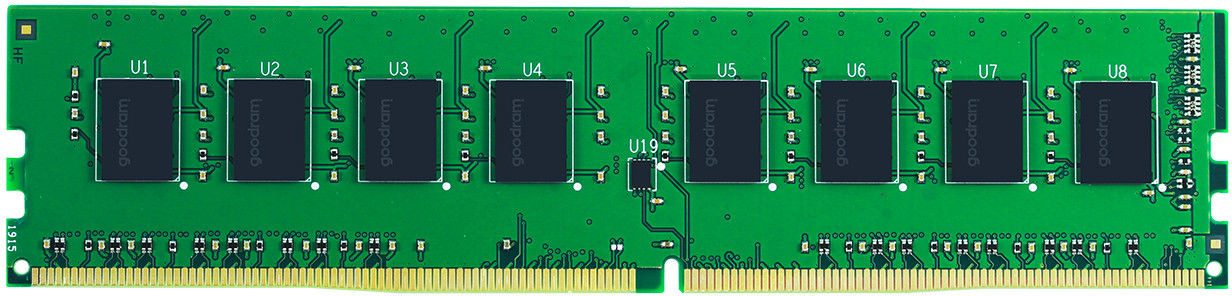
\includegraphics[width=13.5cm]{DIMM.jpg}
  \caption{Un DIMM de mémoire SDRAM DDR4 (largeur=13.5cm). On distingue 8 DRAM chips.\label{fig:DIMM}}
\end{figure}

Les composants matériels qui composent la RAM (hors HBM et eDRAM) se présentent
typiquement sous la forme de \og barrettes\fg~: ce sont les DIMMs (\anglais{Dual
  In-line Memory Module} --- le \og dual\fg vient du fait que les $n$
connecteurs connecteurs du devant ne sont pas reliés à ceux du derrière, ce qui
fait $2n$ connecteurs en tout). Voire fig.~\ref{fig:DIMM}. Un DIMM contient des
circuits intégrés, les \anglais{DRAM chip}s. Sur un DIMM donné, ils sont en
principes tous identiques. Dans les ordinateurs portables, on met des SO-DIMM
(\anglais{Small Outline DIMM}) plus compacts, mais c'est la même chose.

\begin{danger}
  Avant les DIMMs, il y avait les SIMMs (Single \dots), avec seulement 144
  contacteurs répliqués des deux côtés. Ces derniers ont disparu dans les années
  2000.
\end{danger}

Les spécifications des modules de DRAM sont établies par le JEDEC
(\anglais{Joint Electron Device Engineering Council}), un organisme de
standardisation.



\paragraph{DDR} Tous les produits mentionnés ci-dessus sont de la DRAM \og
normale\fg. Depuis l'an 2000, toute la mémoire DRAM est à \og \anglais{Double
  Data Rate}\fg (DDR), c'est-à-dire que sur le \anglais{bus} qui la relie au
contrôleur mémoire, il peut y avoir \emph{deux} \og transfert\fg par cycle (un
lorsque le signal d'horloge \og monte\fg et l'autre lorsqu'il \og
descend\fg). Un transfert est un paquet de données de 64 bits (c'est constant
sur toutes les générations de SDRAM).

Il y a plusieurs générations technologiques successives : DDR, DDR2, DDR3, DDR4,
\dots Elles sont incompatibles, et les DIMMs ont des détrompeurs qui empêchent
de les insérer dans des connecteurs d'une autre génération. Au sein d'une même
génération, il y a des niveaux de performances standardisés
(cf. fig.~\ref{tab:DDR}). Grosso-modo, un module de DDR$x$-$y$ est capable
d'effectuer $y$ Mega-tranferts par seconde, pour une une bande passante de $8y$
Mo/s (puisqu'un \og transfert\fg c'est 64 bits, donc 8 octets). Parfois, la
dénomination commerciale PC$x$-$z$ est utilisée, où $z=8y$ est la bande passante
(en Mo/s) et $y$ désigne la nomenclature \og standard\fg (les deux sont données
dans la \emph{shopping list} ci-dessus, ce qui rend le tout encore plus confus).

Une différence qui n'est pas immédiatement apparente entre les générations est
la notion de \og \anglais{Burst}\fg. Les transferts se font forcément par
paquets de $x$ à des adresses consécutives, où $x$ est le
\anglais{Burst}. Autrement dit, en \the\year, quand on veut lire un octet dans
un module de RAM, il y a forcément 8 transferts de 64 bits, donc 64 octets qui
circulent sur le bus mémoire. On verra section~\ref{sec:cache_line} que ceci est
logique vu l'organisation des caches.

\begin{figure}
  \centering
  \begin{tabular}{|c|c|c|c|c|c|c|}
  \hline
  Génération            & Année                 & Burst              & Standard   & Freq. chips (Mhz) & Freq. bus (Mhz) & Mo/s \\
  \hline\hline                                                                                      
  \multirow{4}{*}{DDR}  & \multirow{4}{*}{2000} & \multirow{4}{*}{2} & DDR-200    & 100               & 100             &  1600 \\
                        &                       &                    & DDR-266    & 133               & 133             &  2133 \\
                        &                       &                    & DDR-233    & 166               & 166             &  2667 \\
                        &                       &                    & DDR-400    & 200               & 200             &  3200 \\
  \hline                                                                                            
  \multirow{5}{*}{DDR2} & \multirow{5}{*}{2003} & \multirow{5}{*}{4} & DDR2-400   & 100               & 200             &  3200 \\
                        &                       &                    & DDR2-533   & 133               & 266             &  4267 \\
                        &                       &                    & DDR2-667   & 166               & 333             &  5333 \\
                        &                       &                    & DDR2-800   & 200               & 400             &  6400 \\
                        &                       &                    & DDR2-1066  & 266               & 533             &  8533 \\
  \hline                                                                                            
  \multirow{6}{*}{DDR3} & \multirow{6}{*}{2007} & \multirow{6}{*}{8} & DDR3-800   & 100               & 400             &  6400 \\
                        &                       &                    & DDR3-1066  & 133               & 533             &  8533 \\
                        &                       &                    & DDR3-1333  & 166               & 667             & 10667 \\
                        &                       &                    & DDR3-1600  & 200               & 800             & 12800 \\
                        &                       &                    & DDR3-1866  & 233               & 933             & 14933 \\
                        &                       &                    & DDR3-2133  & 266               & 1067            & 17067 \\
  \hline                                                                                            
  \multirow{7}{*}{DDR4} & \multirow{7}{*}{2014} & \multirow{7}{*}{8} & DDR4-1600  & 200               & 800             & 12800 \\
                        &                       &                    & DDR4-1866  & 233               & 933             & 14933 \\
                        &                       &                    & DDR4-2133  & 266               & 1066            & 17067 \\
                        &                       &                    & DDR4-2400  & 300               & 1200            & 19200 \\
                        &                       &                    & DDR4-2666  & 333               & 1333            & 21333 \\
                        &                       &                    & DDR4-2933  & 366               & 1467            & 23467 \\
                        &                       &                    & DDR4-3200  & 400               & 1600            & 25600 \\
  \hline                                                                                            
  DDR5                  & 2020 ?                & ?                  & DDR5-6400  & ?                 & 3200            & 51200 \\
  \hline                                                                                            
  DDR6                  & ?                     & ?                  & ?          & ?                 & ?               & \\
  \hline
\end{tabular}
\caption{Standard pour les modules de DRAM. \label{tab:DDR}}
\end{figure}

% buffered, ECC

\paragraph{UDIMM, RDIMM} Un module de RAM peut être \anglais{Unbuffered} (on dit
aussi \anglais{Unregistered} et on parle de UDIMM) ou bien \anglais{Registered}
(on dit aussi \anglais{Buffered} et on parle de RDIMM). Dans le deuxième cas, un
\emph{registre} (c.a.d. un tampon) est présent entre les DRAM chips et le
contrôleur mémoire. Ce tampon joue le rôle de relais et il réduit la quantité de
courant qui circule sur le bus (le contrôleur n'a pas à \og piloter\fg
directement les DRAMs chips). Ceci permet d'augmenter la quantité de DIMMs qu'on
peut brancher sur le même bus et améliore la stabilité globale du système. On
trouve typiquement des UDIMMs dans les ordinateurs personnels et des RDIMMs dans
les serveurs et les machines de HPC. Les RDIMMs sont généralement plus chers, et
le \emph{buffer} ajoute généralement une pénalité d'un cycle aux latences
d'accès à la mémoire. Il existe aussi des LRDIMM (\anglais{Load Reduced} ...),
Une variante améliorée de DIMM à registre (plus récente, depuis 2013,
généralement de plus grande capacité).

Une autre caractéristique que les DIMM peuvent avoir ou pas est la capacité de
correction d'erreur : on parle alors de DIMM ECC (\anglais{Error-Correcting
  Code}). En effet, lors du stockage ou du transfert de 64 bis, un code
correcteur d'erreur permet la correction de n'importe quelle erreur affectant un
seul bit ainsi que la détection d'erreurs affectant deux bits. Le prix à payer
pour cette capacité est qu'il faut stocker et transférer 72 bits au lieu de
64. Un module ECC doit donc avoir une capacité réelle $12.5\%$ plus élevée qu'un
module non-ECC de la même capacité nominale. Les modules ECC se retrouvent
typiquement dans les serveurs et les machines de HPC, rarement dans les
ordinateurs personnels. La gestion du code correcteur peut augmenter un peu la
latence d'accès à la mémoire.

\begin{danger}
  Bien que cela puisse paraître surprenant, la RAM peut en effet exhiber des
  erreurs. Deux phénomènes distincts apparaissent~:
  \begin{enumerate}
  \item Les erreurs \emph{passagères} (\anglais{transient}, \anglais{soft
      error}). Le contenu d'un bit de la mémoire est modifié ponctuellement sous
    l'effet d'interférences electro-magnétiques (\og raysons cosmiques\fg ou
    exposition à la radioactivité), mais à part ça les circuits fonctionnent
    normalement.
    
  \item Les erreurs \emph{permanentes} : le circuit est endommagé et ne stocke
    plus rien correctement.
  \end{enumerate}
  
  Les erreurs passagères sont plus fréquentes qu'on ne pourrait le croire. Les
  ingénieurs de \textsf{Google} ont surveillé l'ensemble de leurs machines
  pendant 2.5 ans~\cite{DRAM-errors-google} : environ un tiers machines est
  affectée par une \og erreur mémoire récupérable\fg (par le code correcteur)
  chaque année, et un peu plus de $1\%$ par une erreur irrécupérable qui fait
  planter la machine et nécessite son remplacement. L'étude note que dans plus
  de 85\% des cas, une erreur récupérable est suivie d'au moins une autre erreur
  récupérable dans le mois qui suit (ce qui laisse supposer que le composant
  matériel va bientôt faillir complètement).

  Le problème est considérablement aggravé dans des environnements radioactifs
  (ou dans l'espace ; l'atmosphère et le champ magnétique terrestre bloquent une
  partie de la radioactivité).
\end{danger}

\begin{ddanger}
  Le code correcteur utilisé est construit à partir du code de Hamming
  $[127, 120, 3]$, qui est un code parfait. L'entrée est tronquée à 64 bits, ce
  qui donne un code $[71, 64, 3]$. Un bit de parité additionnel (le XOR de tous
  les bits d'entrée) est ajouté, ce qui donne un code $[72, 64, 4]$.
\end{ddanger}


\paragraph{Canaux} La DRAM fonctionne essentiellement avec des condensateurs : chargés, ils
contiennent le bit UN ; déchargés, ils contiennent le bit ZÉRO. Il y a cependant
des fuites de courant : ces condensateurs perdent naturellement leur charge au
cours du temps, et il faut donc périodiquement les \emph{rafraichir} en \og
lisant\fg le bit contenu puis en le \og ré-écrivant\fg. Il faut typiquement
faire ceci toutes les 64ms.

La gestion du bon fonctionnement de la DRAM est donc typiquement déléguée à un
contrôleur matériel. Ce dernier gère le rafraîchissement de la DRAM, mais aussi
l'ordonnancement des requêtes, la concurrence, etc. Bref c'est encore très
compliqué.

En \the\year, les contrôleurs mémoire sont généralement \emph{dans} les CPUs,
mais ça n'a pas toujours été le cas. Dans du matériel hau-de-gamme, c'est le cas
depuis plus longtemps, mais pour le matériel \og grand public\fg, c'est depuis
$\approx 2008$ (AMD K8 et Intel \og Nehalem\fg).

Un contrôleur mémoire pilote un ou des canaux (\og \anglais{channel}\fg), sur
lequel sont connecté un ou des DIMMs. Avant $\approx 2000$, un contrôleur
mémoire avait un seul canal. Mais, pour augmenter la bande passante de la
mémoire, le nombre de canaux a inexorablement augmenté : en effet, la bande
passante d'un seul DIMM est limitée (cf. fig.~\ref{tab:DDR}), mais avec $n$
DIMMs sur $n$ canaux, on peut obtenir $n$ fois la bande passante d'un seul DIMM.
Aujourd'hui, les processeurs \og entrée de gamme\fg ont 2 canaux (tous les Intel
Core i3 et Intel Core i5 par exemple). En 2008, les Intel Core i7 920 (\og
Bloomfield\fg) ont trois canaux. En 2012, les Core i7-3820 (\og Série x, Sandy
Bridge\fg) en ont quatre. En 2017, les Xeon SP (\og Skylake\fg) en ont 6 (deux
contrôleurs de trois canaux), tandis que les AMD Epyc en ont huit (4 contrôleurs
à deux canaux), tout comme les IBM Power9.

Il faut noter que ce parallélisme de données permet d'augmenter la bande
passante de la mémoire, mais il ne diminue pas la latence. La façon dont les
adresses physiques sont réparties sur les différents canaux n'est pas
fixée. Elle est parfois configurable dans le micrologiciel de la machine.

Par contre, les DIMMs qui sont branchés sur le même canal ne peuvent pas être
lus/écrits en parallèle. En effet, sur \emph{un} canal il y a \emph{un} bus
% d'adresse/commande et \emph{un} bus de données,
partagé entre tous les DIMMs. Un seul peut lire/écrire sur ce bus partagé à la
fois. Les performances maximales sont donc en principe atteintes avec un seul
DIMM par canal.

\begin{danger}
  Au passage, il y a aussi des limites physiques qui contraignent le nombre de
  DIMMs par canal. Les processeurs Intel et AMD récents ne supportent que deux
  DIMMs par canal, ce qui fait 12 ou 16 DIMMs en tout par processeur.

  Dans les processeurs AMD Epyc, un canal peut fonctionner jusqu'à 2666MHz avec
  \emph{un seul} DIMM, mais la fréquence baisse à 2133MHz si on met \emph{deux}
  DIMMs. Sur les processeurs Intel récents, cette diminution n'est pas
  systématique mais elle peut avoir lieu quand même.

  Donc : a) si on veut vraiment beaucoup de RAM, il faut utiliser beaucoup de
  processeurs, et b) plus on veut de RAM, plus elle est lente.
\end{danger}

% DRAM chips

\paragraph{Rangs} Sur l'image de la figure~\ref{fig:DIMM}, on voit un DIMM
composé de plusieurs \anglais{DRAM chips}. Ces DRAM chips sont groupés par
\emph{rangs}. Un DIMM peut comporter un seul rang, ou bien deux, ou bien quatre
(traditionnellement, les DIMMs à deux rangs ont des \anglais{DRAM chips} des
deux côtés : côté pile, ils forment le rang zéro, et côté face le rang 1 ; mais
il n'y a pas une correspondance stricte entre rangs et côtés). Depuis la DDR4,
il est possible d'avoir huit rangs par DIMM. En pratique, c'est rare en dehors
des LRDIMM de la plus grosse capacité (64/128Go en \the\year). Au sein d'un
rang, tous les \anglais{DRAM chips} sont lus/écris simultanément, en
parallèle. En effet, chaque rang doit être capable de lire/écrire 64 bits de
données \og d'un coup\fg, et pour cela les 64 bits de données sont répartis sur
plusieurs \anglais{DRAM chips}. La configuration la plus courante pour les UDIMM
est de 8 chips qui lisent/écrivent 8 bits par cycle (on parle alors de \og
$\times 8$\fg). La configuration la plus courante dans les RDIMM avec correction
d'erreur est de 18 chips qui lisent/écrivent 4 bits par cycle (on parle alors de
$\times 4$). Là encore, c'est une forme de parallélisme de données qui augmente
le débit, mais pas la latence.

À ce sujet, les \anglais{DRAM chips} fonctionnent à une fréquence moindre que
celle du bus qui relie le DIMM au contrôleur. On voit sur la
figure~\ref{tab:DDR} que leur fréquence n'a que peu évolué depuis l'an 2000
(multiplication par deux), alors que la bande passante totale des DIMMs, elle, a
augmenté de manière plus importante. Or, la latence des accès à la mémoire est
inversement proportionnelle à la fréquence des \anglais{DRAM chips}.

Au passage, sur un canal, le contrôleur ne peut lire/écrire/commander qu'un seul
rang à la fois par cycle d'horloge du bus, car tous les rangs sont branchés \og
en parallèle\fg sur le canal. Mais, comme verra plus bas, les commandes envoyés
par le contrôleur mémoire aux \anglais{DRAM chips} mettent un certain temps à
être exécutées (plusieurs cycles). Pendant qu'un des rangs du canal est \og
occupé\fg, le contrôleur mémoire peut communiquer avec les autres, ce qui
augmente sa capacité à satisfaire des requêtes d'accès à la mémoire. Des
expériences suggèrent qu'avec deux rangs, la latence \og en plein charge\fg des
accès à la mémoire est diminuée de 30\% sur certaines machines par rapport à des
DIMMs comparables à un seul rang. Au-delà de 4 rangs, ce bénéfice est compensé
par le trafic additionnel qui a lieu sur le bus.

\begin{danger}
  Certains processeurs imposent une limite au nombre de rangs qui peuvent
  coexister sur le même canal, par exemple 8 pour certains processeurs Intel.
\end{danger}

% chips, banks, détails crades
\paragraph{Banques, lignes, colonnes} Au bout de la chaine, nous trouvons les
\anglais{DRAM chips}. Chaque norme de DDR spécifie des tailles de chips
standardisées. Dans la norme DDR4, il peut y en avoir de 2, 4, 8 ou 16 Gigabits.

À l'intérieur d'un DRAM chip, les données sont stockées selon un schéma à trois
dimensions : il y a 16 \emph{banques}, chacune constituée d'un tableau à deux
dimensions, avec des \emph{lignes} et des \emph{colonnes}. À la fin, chaque case
contient 4 bits ou 8 bits (selon que c'est un $\times 4$ ou un $\times 8$). Dans
la norme DDR4, les lignes sont toujours de taille 1024 (c.a.d. qu'il y a 1024
colonnes).

\begin{myfilet}
  Si on prend un DIMM \og standard\fg de 16Go, (unbuffered, $\times 8$,
  \anglais{dual-ranked}), possédant 16 \anglais{DRAM chips}, possédant chacun 16
  banques, où chaque \og case\fg contient 8 bits, on trouve qu'il y a
  nécessairement 65536 lignes.
\end{myfilet}

Chaque banque est indépendante. Les commandes adressées par le contrôleur
indiquent quelle banque est visée. Lire ou écrire les données est un processus
en plusieurs étapes ; pour lire ou écrire une adresse donnée, il faut :
\begin{enumerate}
\item Activer la bonne ligne (command ACTivate).
\item Lire ou écrire une colonne de la ligne active (commandes READ/WRITE).
\item Désactiver la ligne active (commande PREcharge).
\end{enumerate}

\medskip

Une seule ligne peut être active simultanément par banque. Il est nécessaire de
désactiver la ligne active avant d'en pouvoir en lire une autre. Les trois
opérations prennent un certain nombre de cycles du \anglais{DRAM chip} : pendant
qu'une banque effectue une opération, cette banque est \emph{occupée} un certain
temps. Mais les autres banques, elles, peuvent être libres (prêtes à recevoir
des commandes). Le contrôleur mémoire doit jongler avec ces contraintes. Dans le
cas de la commande de lecture, le délai est imposé entre l'envoi de la commande
et le moment où les données sont disponibles sur le bus du canal.

Pour simplifier un peu, les choses, dans la norme DDR4, chaque commande
nécessite toujours le même nombre de cycles, et il est généralement noté CL
(dans les normes précédentes, la latence de chaque opérations était
différente). Et ce qui simplifie encore plus les choses, c'est que ça prend
\emph{toujours à peu près le même temps}, quelle que soit la fréquence d'horloge
des \anglais{DRAM chips}, comme le montre la figure~\ref{tab:DDR-lat}. Ceci dit,
des DIMMs de moins bonne qualité peuvent avoir un CL un peu plus élevé que le
minimum légal indiqué dans cette figure.

\begin{figure}
  \centering
  \begin{tabular}{|c|c|c|c|c|}
  \hline
Standard   & Freq. chips (Mhz) & Mo/s  & CL min. & Latence (ns) \\
  \hline\hline                                                                    
DDR4-1600  & 200               & 12800 & 10      & 12.5   \\
DDR4-1866  & 233               & 14933 & 12      & 12.857 \\
DDR4-2133  & 266               & 17067 & 14      & 13.125 \\
DDR4-2400  & 300               & 19200 & 15      & 12.5   \\
DDR4-2666  & 333               & 21333 & 17      & 12.75  \\
DDR4-2933  & 366               & 23467 & 19      & 12.96  \\
DDR4-3200  & 400               & 25600 & 20      & 12.5   \\
  \hline                                                                                            
\end{tabular}
\caption{Standard pour les modules de DRAM. \label{tab:DDR-lat}}
\end{figure}

Une conséquence du mécanisme en trois étapes décrit ci-dessus est que le temps
nécessaire pour lire la mémoire est \emph{variable} : si le contrôleur veut
lire/écrire la ligne $i$ sur une certaine banque, alors trois situations peuvent
se produire :
\begin{itemize}
\item La ligne $i$ est déjà active. Il envoie READ/WRITE. Durée : CL.
\item Aucune ligne n'est active. Il envoie ACTivate puis READ/WRITE. Durée : $2\times$ CL.
\item Une ligne $j \neq i$ est active. Il envoie PREcharge, ACTivate puis READ/WRITE. Durée : $3\times$ CL.
\end{itemize}

\medskip

Par conséquent, les contrôleurs mémoire essaye de minimiser les pénalités dues
au second et au troisième cas, en \emph{réordonnant} les requêtes d'accès à la
mémoire pour maximiser le nombre de \emph{hits} sur les lignes déjà actives. Il
y a 16 banques par \anglais{DRAM chip} à gérer en parallèle (qui peuvent toutes
avoir des lignes actives différentes), ce qui donne des problèmes
d'ordonnancement assez compliqués pour obtenir de bonnes performances.  Le \og
rafraîchissement\fg qui doit être effectué périodiquement par le contrôleur
revient en fait à activer une ligne, effectuer une lecture quelconque, puis
désactiver la ligne. Ceci doit être effectué pour chaque ligne de chaque banque
toutes les 64ms, ce qui rajoute encore des contraintes !

En tout cas, lire des adresses \emph{physiques} contiguës est a priori
légèrement plus favorable que lire des adresses complètement aléatoires, car on
a plus de chance de tomber dans la même ligne. En réalité, ceci est
inexploitable dans les applications, car ces dernières manipulent des adresses
\emph{logiques} qui ne correspondent absolument pas aux adresses physiques (et
que l'OS randomise parfois).

Mais ce qu'on peut dire, c'est que \emph{dans le meilleur des cas}, une requête
de lecture/écriture adressée au contrôleur mémoire ne peut être satisfaite que
12.5ns plus tard, ce qui correspond à 37.5 cycles d'un CPU à 3GHz. Et dans le
pire des cas, c'est au moins trois fois plus. Et en réalité, la latence des
accès mémoire est encore plus importante.

Sous linux, les programmes \texttt{lshw} et \texttt{dmidecode} permettent
d'apprendre des informations intéressantes sur la mémoire installée.

\section{\textsf{STREAM}}

En 1995, John D. McCalpin a conçu un petit programme de test pour mesurer la
bande passante de la mémoire des machines \og vectorielles\fg qui existaient à
l'époque. Son petit programme, \textsf{STREAM}~\cite{McCalpin1995}, a eu
beaucoup de succès et il est toujours utilisé aujourd'hui. Il se compose de
quatre tests décrits figure~\ref{fig:STREAM_description}. Il alloue trois grands
tableaux $A, B$ et $C$ de $N$ flottants double précision, avec $N$ suffisamment
grand pour que les données ne tiennent pas dans les caches de la hiérarchie
mémoire (il est recommandé de choisir $10\times$ la taille du plus grand
cache). Ceci oblige la machine à transférer depuis/vers la RAM et cela permet
donc de mesurer le débit de la mémoire. Les opérations sont vectorisables, et
leur intensité arithmétique est faible (peu d'opérations arithmétiques par
flottant transféré de la mémoire).

\begin{figure}
  \centering
\begin{tabular}{|llcc|}
  \hline
  nom   & opération                             & octet/itération & FLOP/itération \\
    \hline  \hline
  COPY  & $A[i] \gets B[i]$                     & 16 & 0 \\
  SCALE & $A[i] \gets \alpha \cdot B[i]$        & 16 & 1 \\
  SUM   & $A[i] \gets B[i] + C[i]$              & 24 & 1 \\
  TRIAD & $A[i] \gets B[i] + \alpha \cdot C[i]$ & 24 & 2 \\
    \hline
\end{tabular}

\caption{Les tests effectués par le \textsf{STREAM} benchmark. Pour tout
  $0 \leq i < N$, l'opération est effectuée. Le nombre $\alpha$ est un flottant
  double précision fixé. \label{fig:STREAM_description}}
\end{figure}

La figure~\ref{fig:STREAM_results} montre le résultat du \textsf{STREAM}
benchmark sur quelques machines. Cela met en évidence le \og \emph{memory
  wall}\fg : sur un laptop conventionnel ou un Raspberry Pi, un seul coeur
suffit à saturer la bande passante de la mémoire.

Sur les machines dédiées au caclul scientifique, qui sont mieux équilibrées, ce
n'est pas le cas. Ceci dit, sur un noeud de BlueGene/Q (une machine qui date de
2011), un quart des coeurs disponibles suffit à saturer la RAM, tandis que sur
un noeud d'un cluster récent, équipé de processeurs Xeon Gold, la moitié des
coeurs suffit à saturer la RAM.

Cela signifie concrètement que sur des machines contemporaines, si les calculs
nécessitent l'accès à de grande quantité de données, alors les unités
d'exécution des processeurs vont passer (au moins) la moitié de leur temps à
attendre l'arrivée des données !

\begin{danger}
  Voici un commentaire un peu plus approfondi des résultats. Le laptop possède
  un SO-DIMM de DDR4-2133 (unbuffered), 2 rangs $\times 8$. La bande passante
  maximale théorique est donc 17Go/s. On atteint $80\%$ du maximum.

  Le \texttt{raspberry Pi 3B+} possède 1Go de LPDDR2-800 (\anglais{Low-Power
    DDR2}), donc possède une bande passante théorique maximale de 6.4Go/s. On
  plafonne à 42\% du maximum théorique, mais il s'agit d'une machine à
  35\euro...
  
  L'IBM BlueGene/Q possède deux contrôleurs à deux canaux, sur lesquels sont
  branchés des chips de DDR3-1333 avec correction d'erreur renforcée. La bande
  passante maximale théorique est donc $4 \times 10.6 = 42.7Go/s$. On atteint
  65\% du maximum.
  
  Le \anglais{cluster node} possède deux processeurs. Le test a été effectué en
  forçant le système d'exploitation à n'en utiliser qu'un seul, pour éviter les
  effets NUMA (la machine a 192Go de RAM, mais chaque processeur n'est
  directement relié qu'à 96Go) --- ceci peut se faire avec la commande
  \verb|numactl --cpunodebind=0|. Chaque processeur a deux contrôleurs mémoire
  de trois canaux chacuns. Chaque canal est équipé d'un RDIMM de DDR4-2666 de
  16Go, \emph{dual-rank}. La bande passante maximale théorique pour un
  processeur est donc de $6 \times 21.3 = 128$Go/s. On voit qu'on atteint
  $65\%$ du maximum.
\end{danger}

\begin{ddanger}
  Au passage, dans le cas du \anglais{cluster node}, le processeur (un Intel
  Xeon Gold 6130 CPU @ 2.10GHz) possède 16 coeurs physiques et
  l'hyper-threading. Faire le \textsf{STREAM} benchmark avec 16 ou 32 threads ne
  change rigoureusement rien~: c'est le débit de la mémoire qui est saturé,
  point final. On peut aussi essayer de faire le test avec 16 threads logiciels
  placés sur 16 coeurs physiques différents, ou bien 16 threads logiciels placés
  sur 8 coeurs physiques différents seulement : la différence n'est pas énorme
  (82.8Go/s vs 75.8Go/s).

  En essayant sur les deux processeurs à la fois, on obtient des résultats
  variables en utilisant seulement un thread par coeur physique (de 85Go/s à
  160Go/s selon les exécutions). Par contre, en utilisant tous les
  hyper-threads, on obtient bien systématiquement 155Go/s, donc un
  quasi-doublement par rapport l'utilisation d'un seul CPU. Mais il est alors
  nécessaire d'utiliser tous les hyper-threads...
\end{ddanger}


\begin{figure}
  \centering
\begin{tabular}{|cc|cccc|c|}
  \hline
  Machine   & Threads & COPY & SCALE & SUM & TRIAD & TRIAD speedup w.r.t. 1 thread\\
    \hline  \hline
  Laptop    & 1 & 13.8 & 9.7 & 10.9 & 10.9 & -\\
  Laptop    & 2 & 13.8 & 9.7 & 10.9 & 10.9 & 1 \\
  \hline
  Raspberry    & 1 & 2.7 & 2.4 &  2.2 &  1.8 & - \\
  Raspberry    & 2 & 2.4 & 2.3 &  2.3 &  2.3   & 1.3 \\
  Raspberry    & 4 & 2.1 & 2.0 &  2.0 &  2.0   & 1.1 \\
  \hline
  BlueGene/Q      & 1  & 5   & 5.5   & 7.5   & 7.5  & -\\ 
  BlueGene/Q      & 2  & 10.5 & 11.2 & 15    & 15   & 2\\
  BlueGene/Q      & 4  & 21.4 & 22.6 & 26.8  & 26.8 & 3.6 \\
  BlueGene/Q      & 8  & 26.3 & 25.9 & 27.6  & 27.9 & 3.7 \\
  BlueGene/Q      & 16 & 26.2 & 26.2 & 28.0  & 28.0 & 3.7 \\ 
  \hline
  Cluster node   & 1  & 10.5 & 12.2 & 12.8 & 12.7 & - \\
  Cluster node   & 2  & 20.5 & 23.8 & 24.8 & 24.6 & 1.9 \\
  Cluster node   & 4  & 39.7 & 45.6 & 48.1 & 47.8 & 3.7 \\
  Cluster node   & 8  & 75.3 & 60.0 & 67.7 & 67.6 & 5.3 \\
  Cluster node   & 16 & 83.2 & 65.4 & 73.5 & 73.4   & 5.7 \\
  \hline
\end{tabular}

\caption{Quelques résultats du STREAM benchmark : débit de la RAM en Go/s.  Le
  \og laptop\fg et le \og Raspberry\fg sont décrits dans la
  figure~\ref{fig:arch1}. La machine \og BlueGene/Q\fg est décrite
  figure~\ref{fig:arch4}. Le \og cluster node\fg est décrit
  figure~\ref{fig:arch2}.\label{fig:STREAM_results}}
\end{figure}

\section{Débit et latence}

En fait, la situation est pire que ce qui est suggéré ci-dessus. Le \emph{débit}
(ou encore la \og bande passante\fg) de la mémoire est une chose, mais sa
\emph{latence} en est une autre, comme en témoigne un examen attentif des deux
figures~\ref{fig:memwall_bw} et~\ref{fig:memwall_lat}. Même si on accède à peu
de données, on risque de devoir les attendre quand même. Les algorithmes de
parcours de graphe forment un exemple typique de ce problème : il faut en
permanence lire de petits paquets de données éparpillés dans toute la mémoire,
et donc payer à chaque fois la latence des accès.

\paragraph{Le modèle RAM est une simplification}Lorsqu'on étudie un algorithme
(séquentiel), on considère généralement que cet algorithme va être exécuté sur
une machine dont le modèle abstrait est la \textit{Random-Access Machine} : une
machine qui a accès à une mémoire, c'est-à-dire un un tableau (généralement
illimité) de cases de $w$ bits chacune. Les \og opérations élémentaires\fg de
cette machine sont la lecture et l'écriture d'une case en mémoire ainsi que les
opérations arithmétiques usuelles sur des mots de $w$ bits (on peut prendre
$w=64$ de nos jours).

La complexité d'un algorithme est généralement décrite comme le nombre
d'opérations élémentaires qu'une telle machine doit effectuer pour
l'exécuter. Ce modèle abstrait a l'avantage d'être simple, mais l'inconvénient
de ne pas décrire fidèlement la réalité, en tout cas pas tout le temps. Plus
précisément, il n'est pas pas faux de dire que, sur une machine donnée, exécuter
l'instruction~:

\mint{C}{double x = A[i];}

prend un temps qui, dans le pire des cas, est borné par une constante
indépendante de $i$. Mais la réalité, c'est que le temps au bout duquel la
valeur de $x$ sera disponible va dépendre de $i$ car la mémoire est organisée de
manière \emph{hiérarchique}. Pour obtenir de bonnes performances, il faut
absolument exploiter cette structure pour éviter de se trouver dans le pire cas,
c'est-à-dire le cas où la valeur de \texttt{A[i]} doit être transférée depuis
une barette de RAM jusqu'aux unités d'exécution du CPU.

\paragraph{Limites physiques} D'un point de vue asymptotique, l'idée qu'on peut
accéder à une quantité arbitraire de mémoire en temps constant se heurte de
toute façon aux réalités du monde matériel. Comme l'information ne peut
(\textit{a priori}) pas se déplacer plus vite que la vitesse de la lumière, et
qu'il ne peut y avoir qu'une quantité finie de bits de mémoire dans un volume
donné, alors plus on a de mémoire et plus une partie de cette dernière est \og
loin\fg, donc plus ça prend de temps d'y accéder. Si $M$ bits de mémoire étaient
disposée dans une boule autour d'une unité de calcul, alors dans le pire des cas
cette dernière ne pourrait accéder aux bits \og externes\fg qu'en attendant un
temps proportionnel au rayon de la boule, donc à $\sqrt[3]{M}$. De nos jours,
les ordinateurs sont plutôt disposés \og à plat\fg, donc en réalité ce serait
plutôt $\sqrt{M}$. Tout ça pour dire que le modèle RAM, qui affirme que c'est
constant, ne peut prétendre au réalisme.

En pratique, on observe empiriquement que plus une machine a de RAM, plus la
latence de cette mémoire est élevée.

\paragraph{Un micro-benchmark} Pour illustrer ceci, on va se pencher sur un
autre micro-benchmark qui stresse la mémoire, le \emph{pointer-chasing}. On
alloue un tableau $T$ de taille $N$, et on l'initialise préalablement avec une
permutation pseudo-aléatoire des entiers $\{0, 1, \dots, N-1\}$\footnote{On
  vérifie que le cycle de la permutation qui commence en zéro est au moins de
  taille $N/3$, sinon on change la permutation. Ça n'arrive pas très souvent :
  la longueur moyenne du cycle auquel appartient un élément aléatoire dans une
  permutation aléatoire de $N$ éléments est $(N+1)/2$ (cf. \cite[§1.3.3,
  exercice 24]{knuth}).}. Ensuite, on mesure le temps d'exécution du bout de
code suivant :
\begin{minted}{C}
int x = 0;
for (int i = 1000000000; i != 0; i--)
	x = T[x];
\end{minted}

Ce bout de code ne fait rien d'autre qu'accéder à la mémoire, mais contrairement
au \textsf{STREAM} benchmark qui accède à zones contiguës de la mémoire, de
manière régulière, ici on charge des adresses \emph{imprévisibles}. De plus, le
programme ne peut pas progresser tant que la valeur de \texttt{T[x]} n'est pas
disponible.

Dans le modèle RAM, le temps d'exécution ne devrait pas dépendre de $N$.  Or,
dans la pratique, il en dépend très sensiblement. C'est d'ailleurs facile à
mesurer. Sur un Raspberry Pi modèle \texttt{3B+}, le compilateur
\texttt{gcc~8.3.0} produit un code assembleur de 3 instructions seulement pour
la boucle critique :
\begin{minted}{asm}
; r4 == adresse de T, r9 == x, r5 == i
loop:
        ldr     r9, [r4, r9, lsl #2]         ; x := *(T + 4*x)
        subs    r5, r5, #1                   ; i := i - 1
        bne     loop                         ; if i != 0 then GOTO loop
\end{minted}

Le processeur Cortex A53 du Raspberry Pi 3B+ est \emph{in-order} et il exécute
une instruction par cycle d'horloge dans le meilleur des cas. Si tout se passait
bien, une itération de la boucle nécessiterait donc 3 cycles d'horloge. Voyons
ce qu'il en est sur la figure~\ref{fig:chasing_pi}~: on voit que c'est bien le
cas tant que les données occupent moins de 32Ko. Par contre, la latence des
accès mémoire est multipliée par $\approx 130$ lorsque la taille des données
passe de de 32Ko à 800Mo.

On observe sensiblement le même résultat sur des machines dédiées au calcul
scientifique (cf. fig.~\ref{fig:chasing_gr20}). En outre, sur ces machines qui
ont beaucoup de RAM, on observe un doublement progressif de la latence au-delà
de 1Go de mémoire à laquelle on accède aléatoirement. La forme des courbes
obtenue résulte de plusieurs phénomènes qu'on va analyser séparément.


\begin{figure}
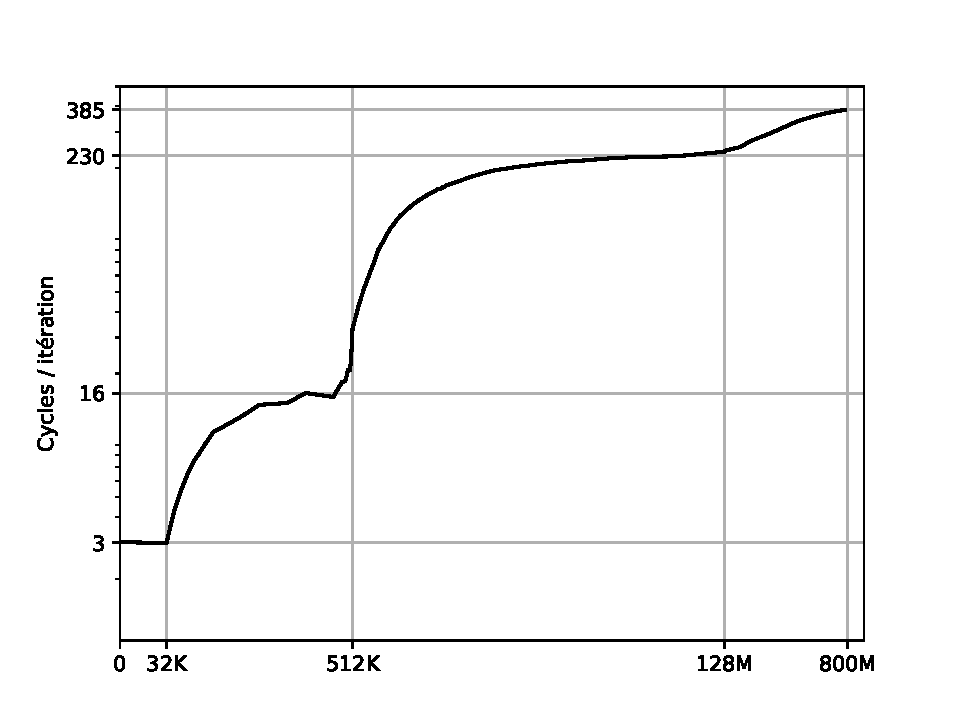
\includegraphics[width=\textwidth]{cache_curve_pi3b.pdf}
\caption{Résultat du \emph{pointer chasing} benchmark sur un Raspberry Pi
  \texttt{3B+}. L'axe des abscisses représente la taille du tableau $T$ en
  octets. \label{fig:chasing_pi}}
\end{figure}

\begin{figure}
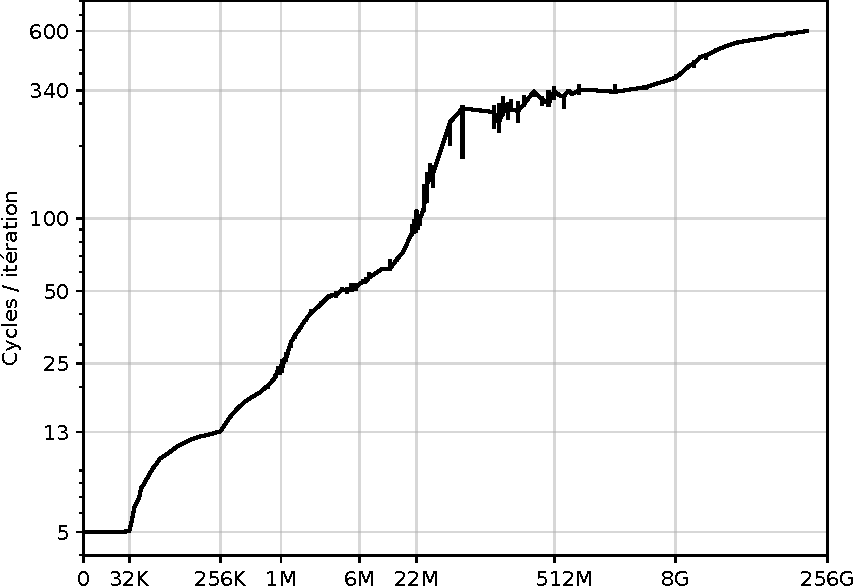
\includegraphics[width=\textwidth]{cache_curve_gr20.pdf}
\caption{Résultat du \emph{pointer chasing} benchmark sur le \og \anglais{cluster node}\fg (décrit fig.~\ref{fig:arch2}). \label{fig:chasing_gr20}}
% ATTENTION : ceci a été obtenu avec des small pages !
\end{figure}

\paragraph{Accès contigus et aléatoires} Mais il y a déjà un phénomène important
qu'on peut constater : sur un coeur de ce \anglais{cluster node}, le programme
\textsf{STREAM} mesure une bande passante mémoire de 10--12 Go/s sur un coeur
(cf. figure~\ref{fig:STREAM_results}). Ceci est obtenu en effectuant des accès
mémoire \emph{contigus} (à des adresses successives). À 3Ghz, cela signifie le
transfert de 4 octets par cycle d'horloge de la RAM vers le CPU.

Mais par contre, ce que montre la figure~\ref{fig:chasing_gr20}, c'est que si on
lit des adresses \emph{aléatoires} dans un tableau qui occupe 512Mo, alors on va
lire un mot de 4 ou 8 octets tous les 340 cycles. Autrement dit, à 3GHz, la
bande passante observée en faisant des accès aléatoires est d'environ 70Mo/s !

La bande passante \og aléatoire\fg est donc 170 fois moindre que la bande
passante \og contigüe\fg. Par conséquent, il est parfois justifié de modifier
les algorithmes pour obtenir des accès mémoires contigus.


\section{Hiérarchie mémoire : les caches}

Pour accélérer les accès à la mémoire, les ordinateurs disposent de \emph{cache}
: de petites mémoires rapides (et chères) placées plus près des unités
d'exécution. Il peut y en avoir plusieurs montés en cascade : dans ces cas-là on
parle du cache de \og niveau 1\fg (\anglais{Level 1} ou L1, celui qui est le
plus proche des unités d'exécution), puis de niveau 2, puis de niveau 3,
etc. (les caches de niveau 4 sont rares de nos jours). Généralement, les caches
les plus proches sont plus rapides et plus petits que les caches les plus
éloignés, pour des raison de coût et de complexité des circuits.

La taille des caches et leurs caractéristiques varient sensiblement d'une
machine à l'autre. Le programme \texttt{lstopo}, qui fait partie de la bibliothèque
\texttt{hwloc} qui fait elle-même partie de \textsf{OpenMPI} permet d'afficher
la hiérarchie mémoire. Les figures~\ref{fig:arch1}, \ref{fig:arch2}
et~\ref{fig:arch3} montrent la hiérarchie mémoire de plusieurs machines assez
différentes : on voit qu'il y a une grande variabilité.

\begin{danger}
  Une partie du fonctionnement de la hiérarchie mémoire des processeurs n'est
  pas, ou mal documenté. De toute façon, c'est très compliqué dès qu'on rentre
  dans les détails et ce document ne prétend d'ailleurs pas à l'exhaustivité !
\end{danger}

\begin{figure}[htpb]
      \centering
  \begin{subfigure}[t]{0.4\textwidth}
    \centering
    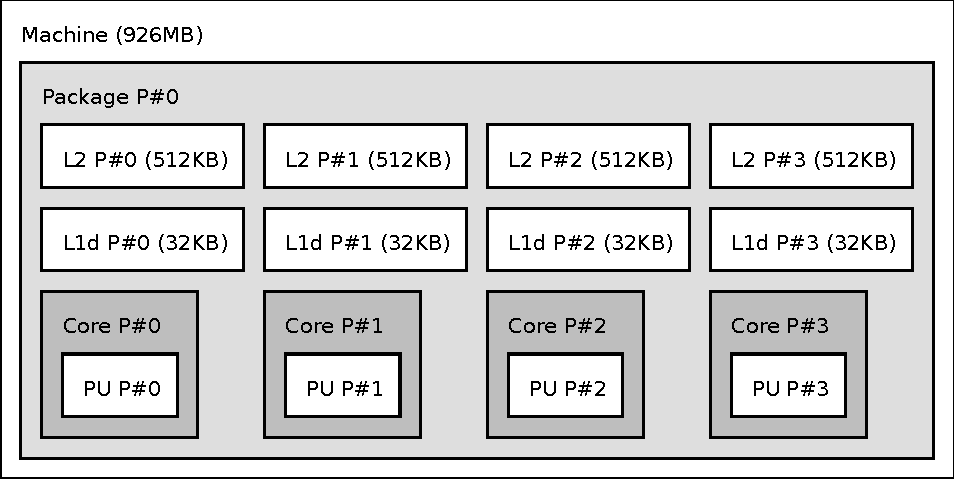
\includegraphics[width=\textwidth]{lstopo_rpi3b.pdf}
    \caption{Un processeur (ARM Cortex A53), quatre coeurs. Chaque coeur possède
      32Ko de cache L1 et 512Ko de cache L2.}
  \end{subfigure}
  \hspace{5mm}
  \begin{subfigure}[t]{0.4\textwidth}
        \centering
    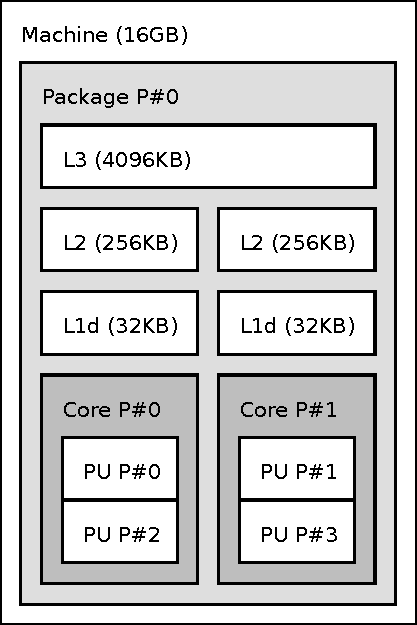
\includegraphics[width=3cm]{lstopo_laptop.pdf}
    \caption{Un processeur (Intel Core i7 6600U), deux coeurs, deux threads
      matériels par coeur. Chaque coeur possède 32Ko de cache L1 partagé entre
      les deux threads ainsi que 256Ko de cache L2. Le processeur contient un
      cache L3 de 4Mo partagé entre les deux coeurs.}
  \end{subfigure}
  \caption{À Gauche, un Raspberry Pi modèle \texttt{3B+}. À droite, le laptop du prof. \label{fig:arch1}}
\end{figure}


\begin{figure}
  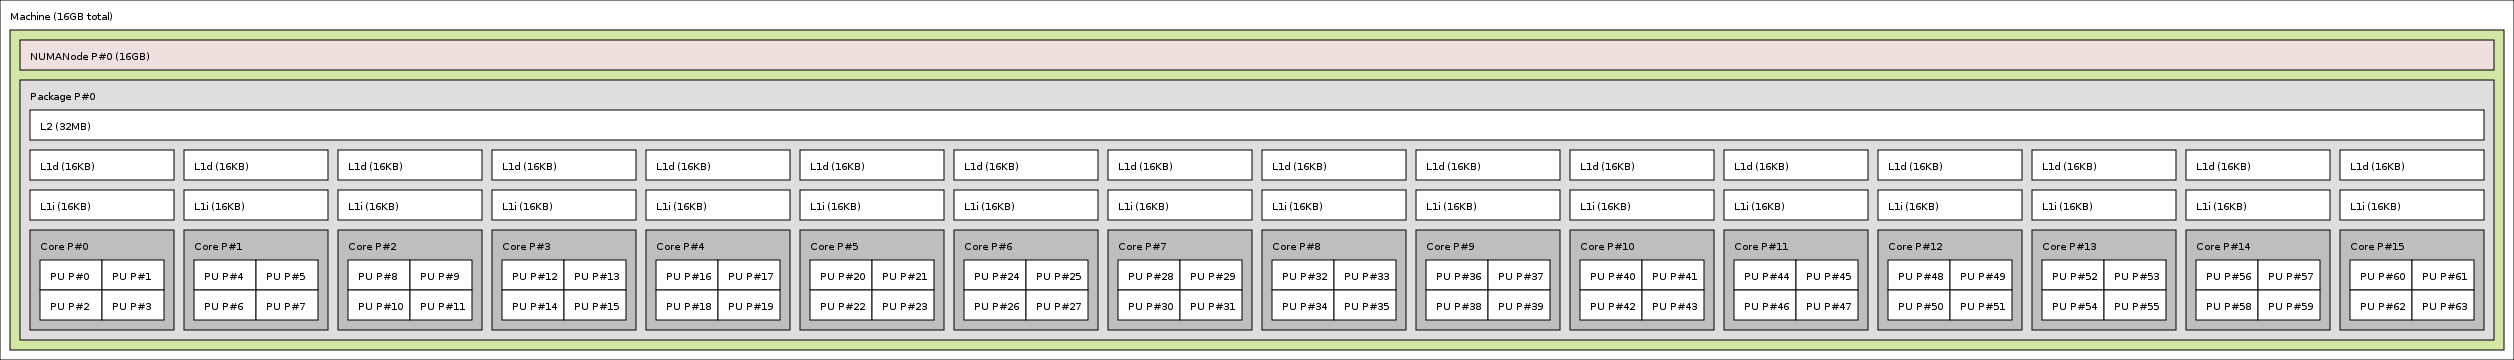
\includegraphics[width=\textwidth]{lstopo_bgq.png}
  \caption{Un noeud de calcul d'une machine massivement parallèle IBM
    BlueGene/Q. Un processeur (PowerPC A2) de 16 coeurs, 4 threads SMT par
    coeur. Chaque coeur possède 16Ko de cache L1, partagé entre les 4 threads
    (c'est peu). Un énorme cache L2 de 32Mo est partagé entre tous les
    coeurs.\label{fig:arch4}}
\end{figure}



\begin{figure}
  \centering
  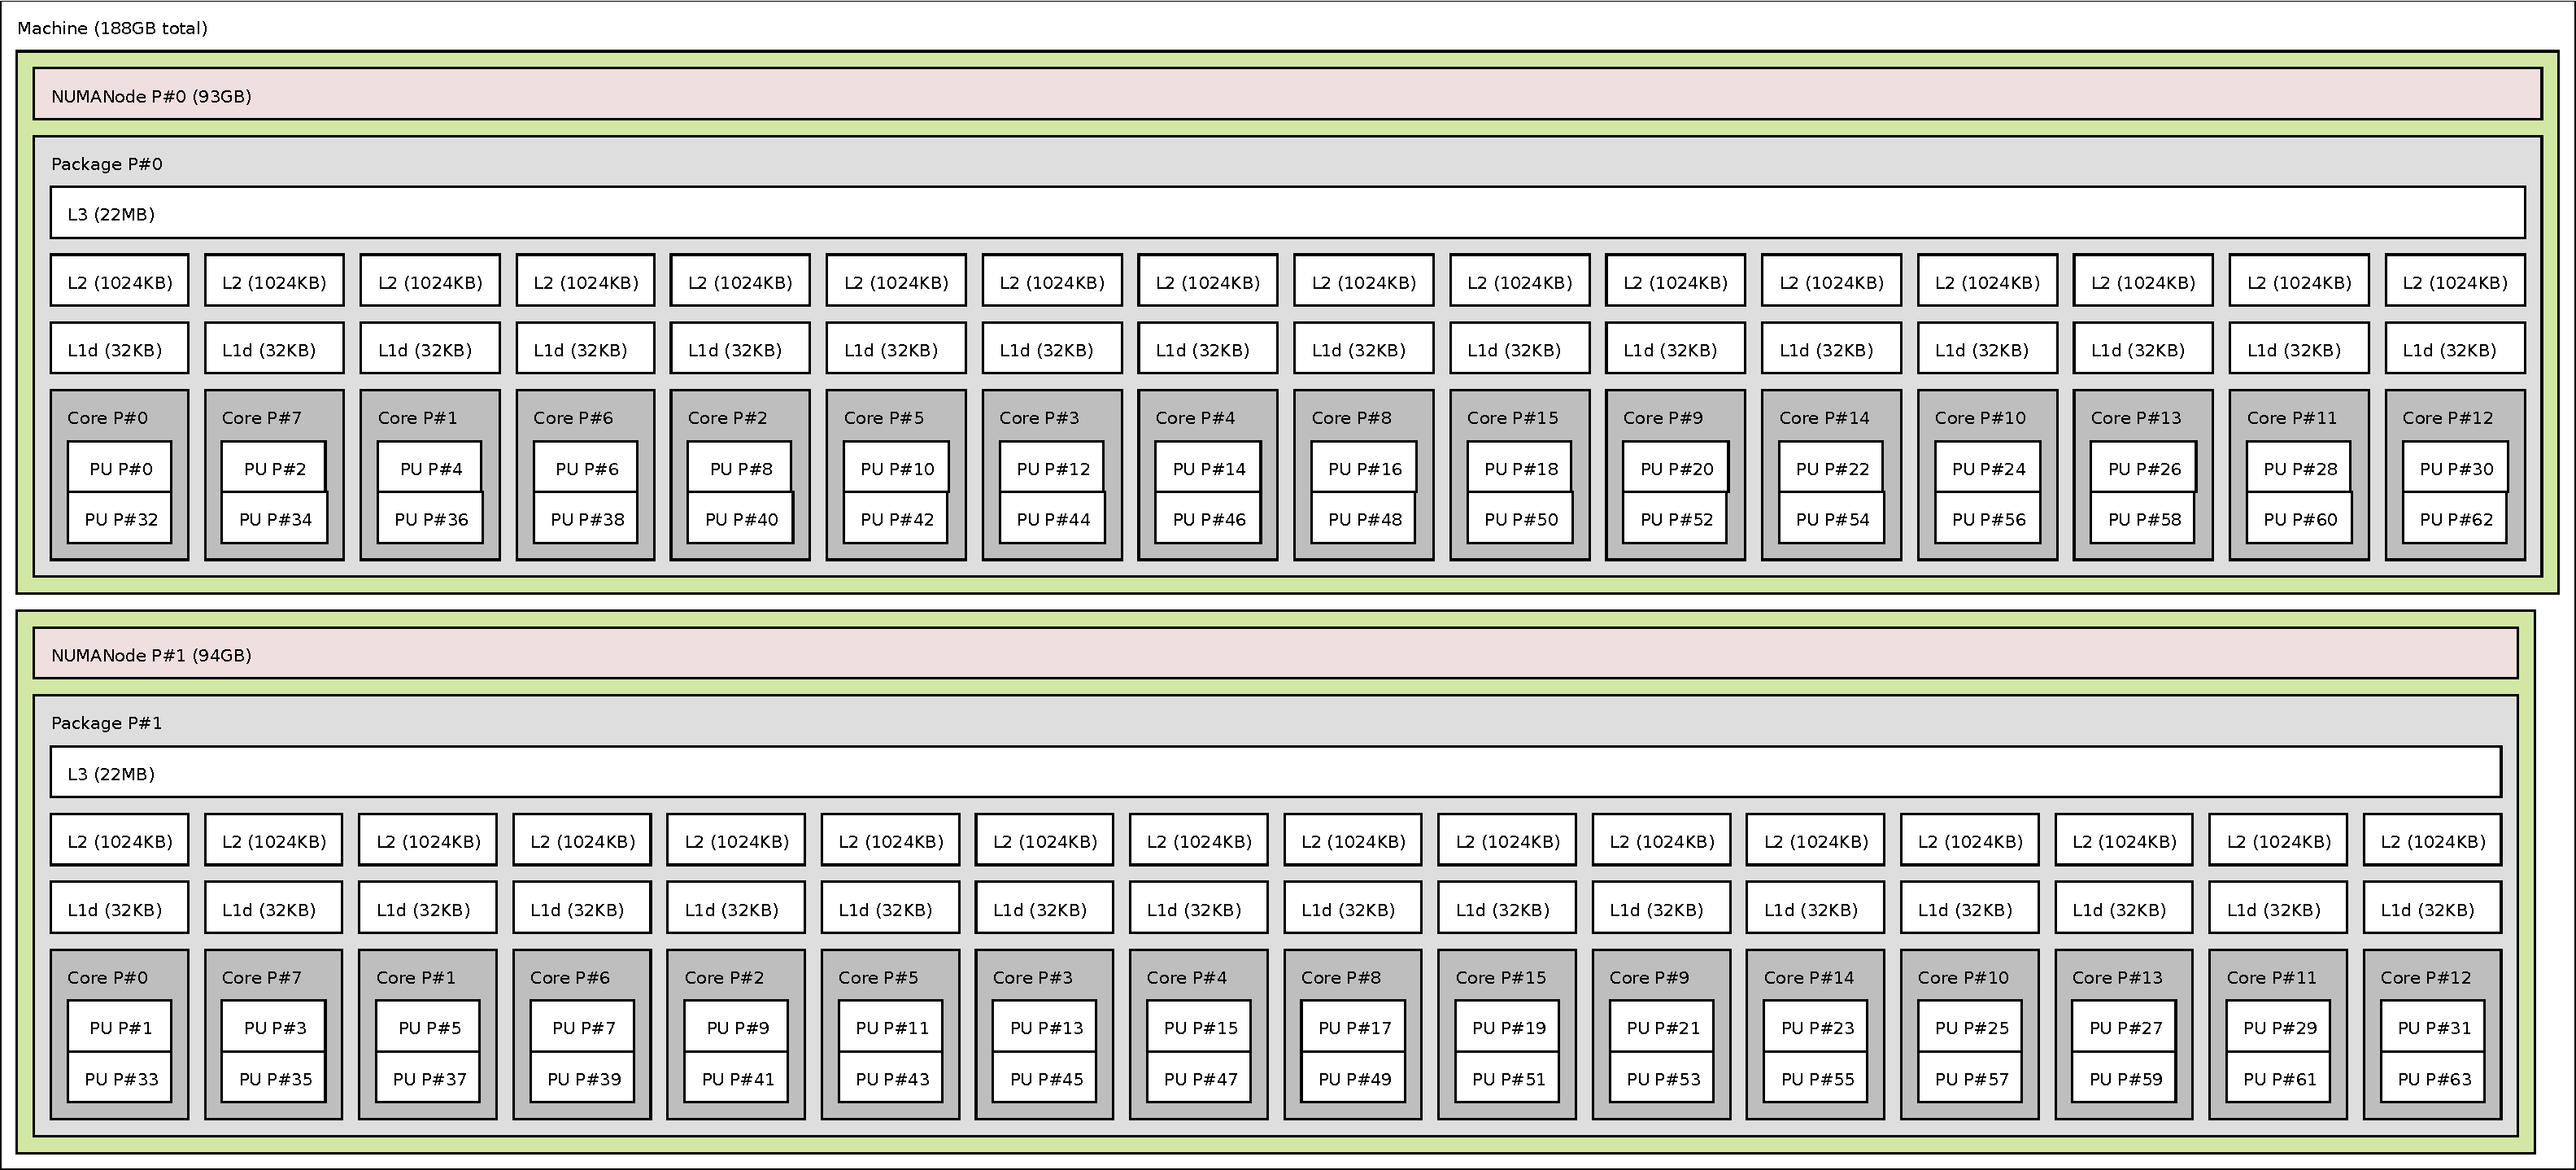
\includegraphics[width=\textwidth]{lstopo_gr20.pdf}
  \caption{Un noeud de calcul d'un cluster récent (2018). Deux processeurs
    (Intel Xeon Gold 6130), 16 coeurs par processeur, deux threads SMT par
    coeur. Chaque coeur possède 32Ko de cache L1 (partagé entre les 2 threads)
    et un gros cache L2 de 1Mo. Un cache L3 de 22Mo est partagé entre tous les
    coeurs. Chaque processeur possède son propre controlleur mémoire et accède
    de manière privilégiée à \og ses\fg 96Go de RAM. Il y a donc deux noeuds
    NUMA.\label{fig:arch2}}
\end{figure}

\begin{figure}
  \centering
  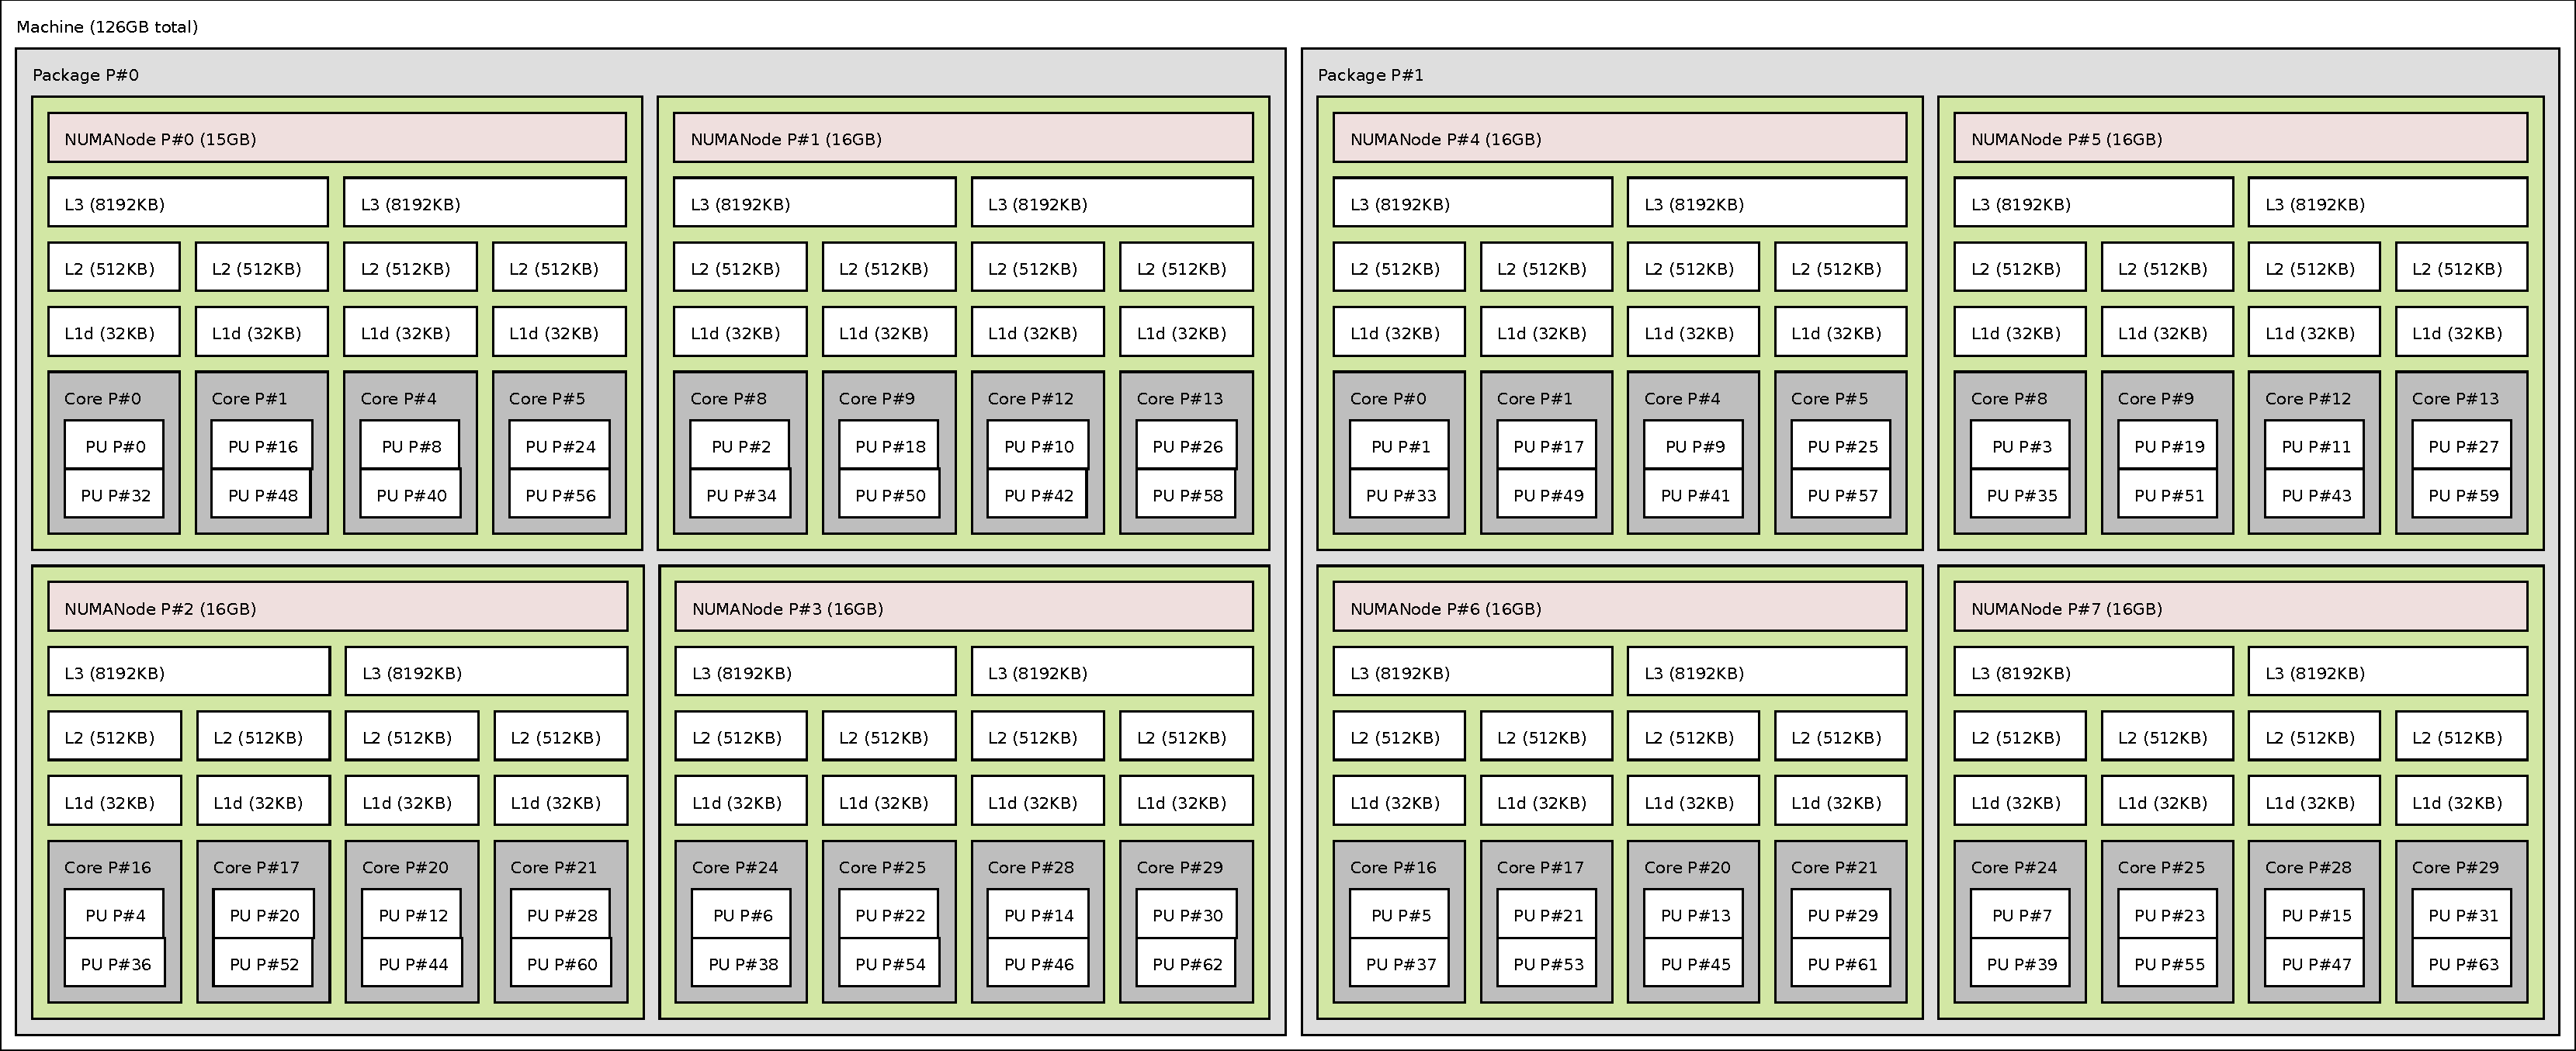
\includegraphics[width=\textwidth]{lstopo_chiclet.pdf}
  \caption{Un autre noeud de calcul d'un autre cluster récent (2018). Deux
    processeurs (AMD EPYC 7301), 16 coeurs par processeur, deux threads SMT par
    coeur. Chaque coeur possède 32Ko de cache L1 (partagé entre les deux
    threads) et 512Ko de cache L2. Chaque \emph{paire} de coeurs partage un
    cache L3 de 8Mo. Chaque processeur est divisé en quatre \og chipplets\fg qui
    ont chacun leur propre controleur mémoire et qui accèdent de manière
    privilégiée à \og leurs\fg 16Go de RAM. Chaque processeur contient donc 4
    noeuds NUMA, et il y a donc huit en tout dans la machine.\label{fig:arch2}}
\end{figure}


\begin{figure}
    \centering
  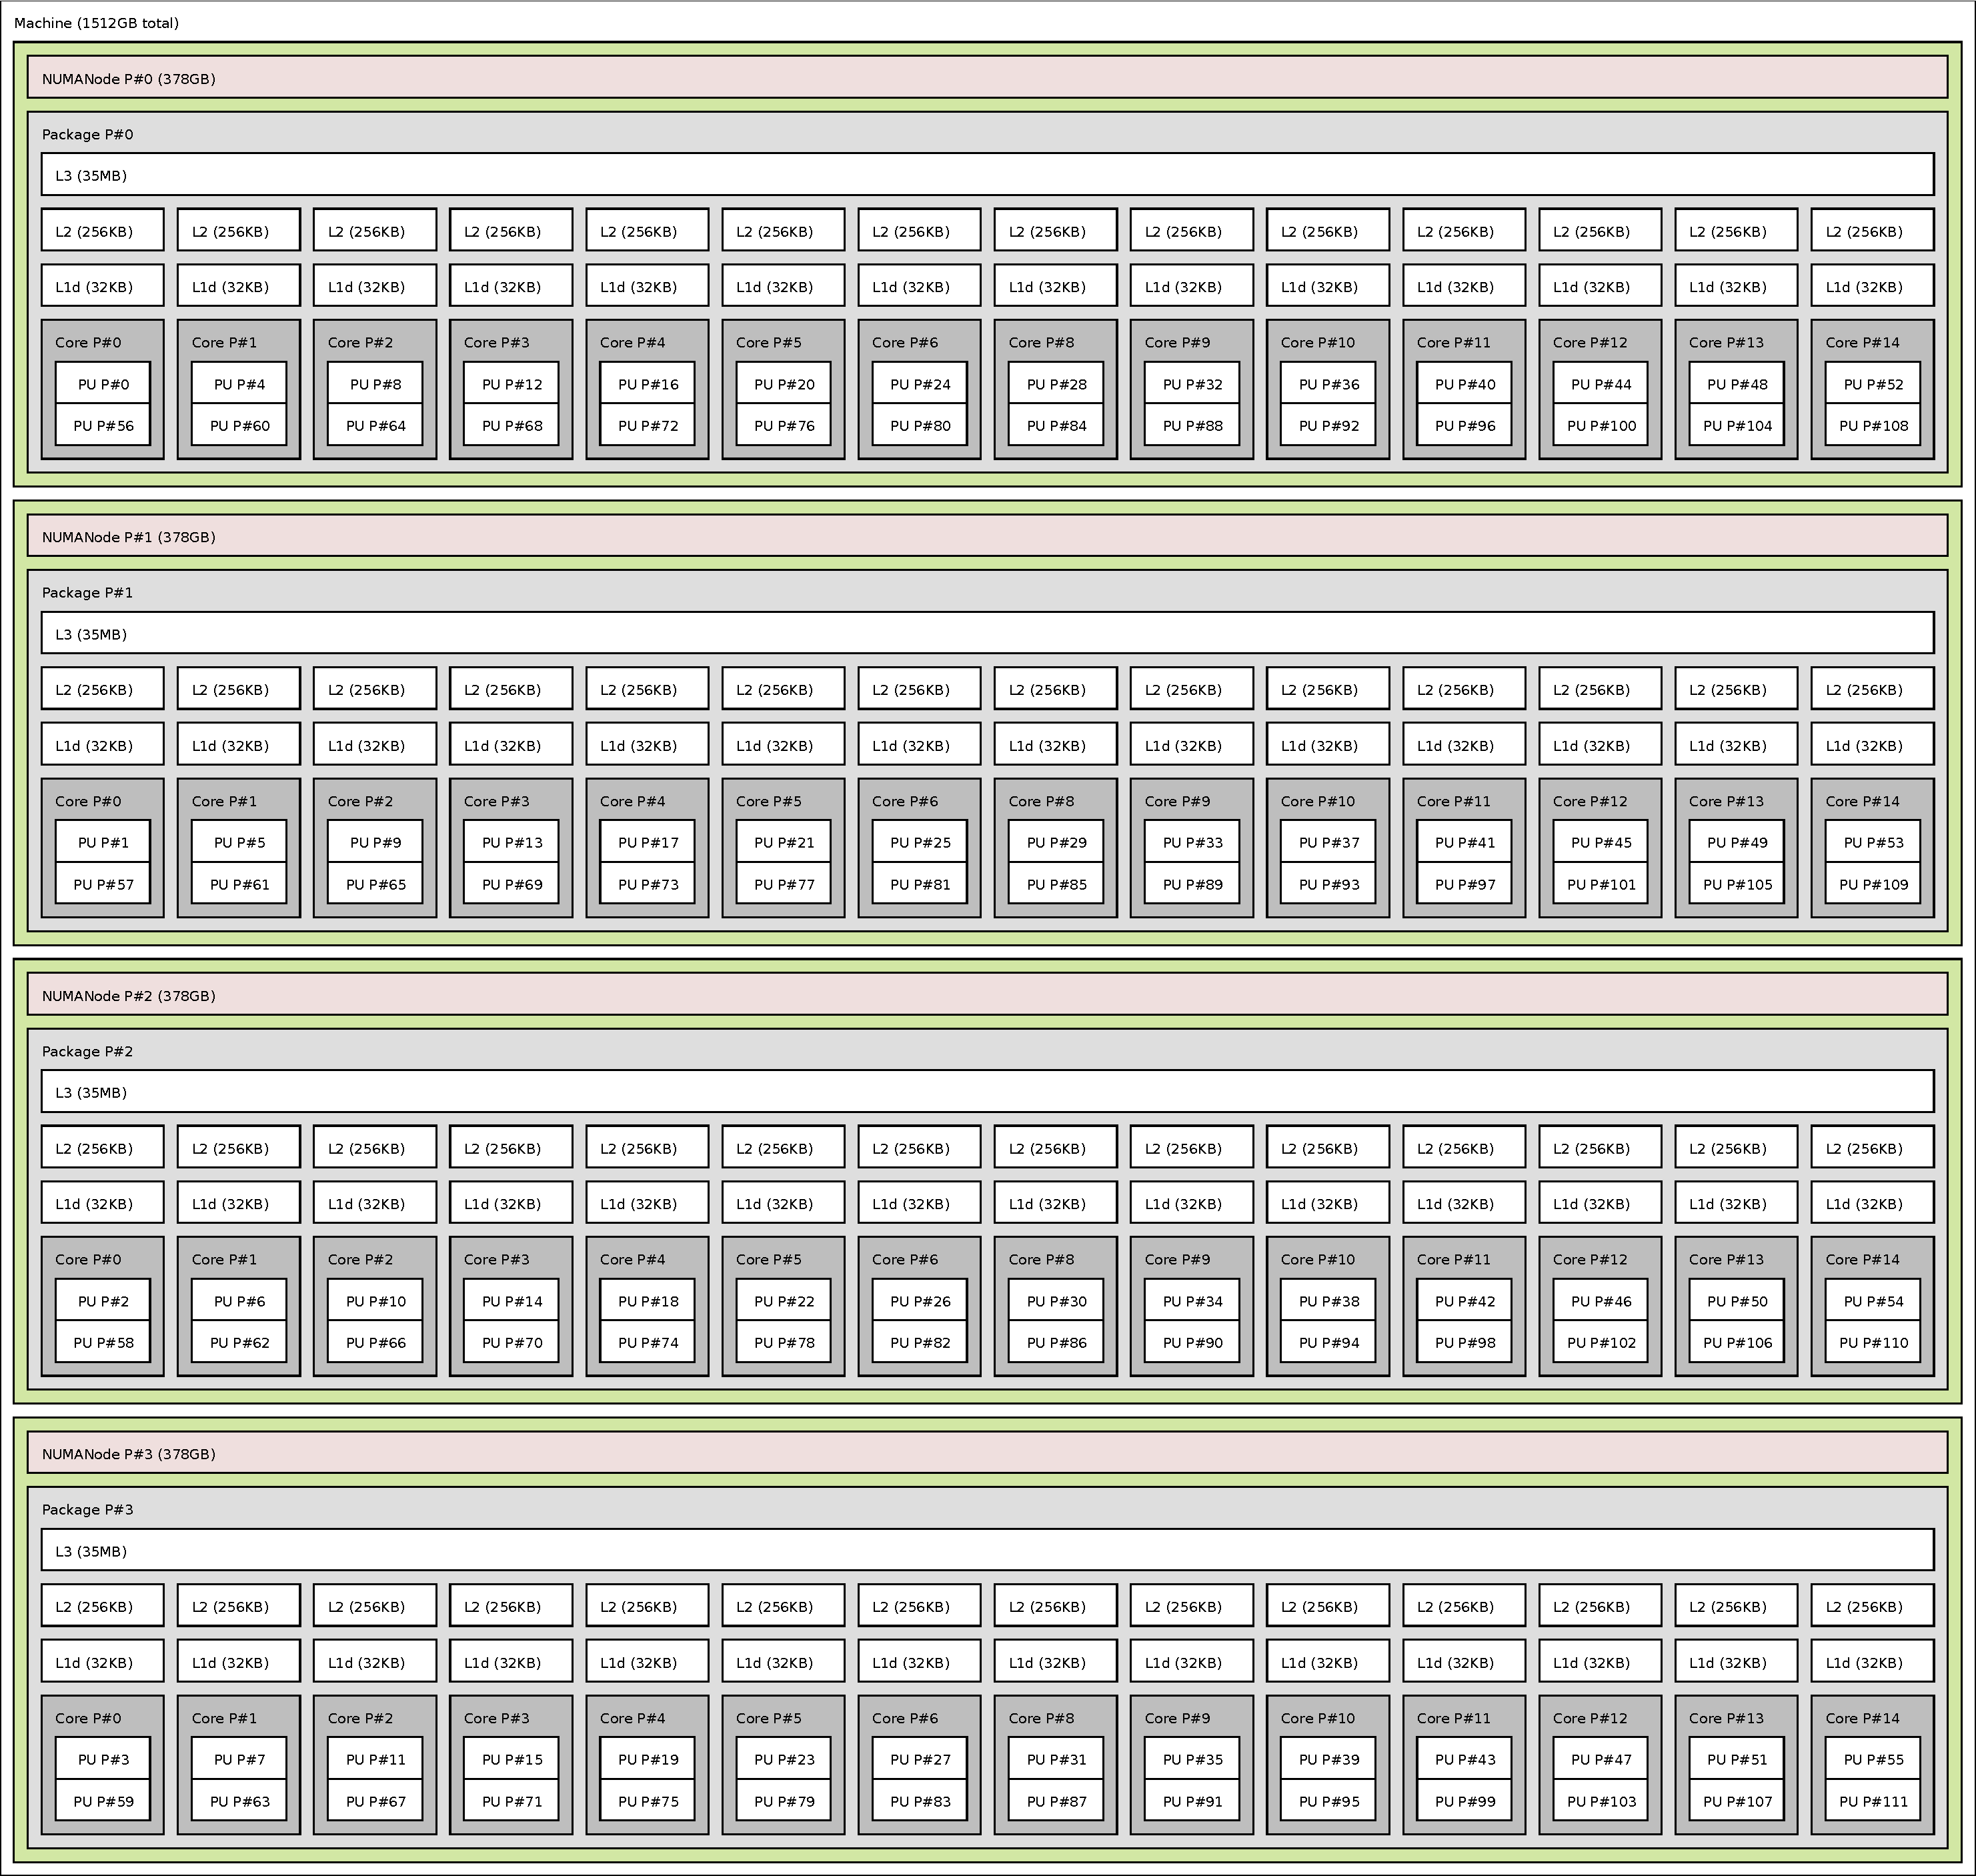
\includegraphics[height=0.5\textheight]{lstopo_wurst.pdf}
  \caption{Un \og fat node\fg pour les calculs qui demandent beaucoup de
    mémoire. Quatre processeurs (Intel Xeon E7-4850 v3), 14 coeurs par
    processeur, deux threads SMT par coeur. Chaque coeur possède 32Ko de cache
    L1 (partagé entre les deux threads SMT) et 256Ko de cache L2 (cette
    configuration était courante pendant des années sur les processeurs
    Intel). Chaque processeur a un cache L3 de 35Mo partagé entre tous les
    coeurs. Chaque processeur contrôle \og ses\fg 384Go de RAM, il y a donc 4
    noeuds NUMA.\label{fig:arch3}}
\end{figure}

Pour obtenir le contenu d'une adresse mémoire, les unités d'exécution du
processeur adressent une requête au cache L1. Si l'adresse demandée est présente
dans le cache, il y a un \emph{cache hit} et la valeur demandée est renvoyé
rapidement. Sinon, il y a une \og faute de cache\fg (\emph{cache miss}) et le
cache L1 s'adresse à l'étage du dessus pour obtenir lui-même la valeur présente
en mémoire à l'adresse voulue. Une fois qu'il la reçoit, il la stocke. Tout ceci
entraîne un temps d'attente supplémentaire.

S'il y a un cache L2, le même mécanisme se répète dans le cache L2, puis
éventuellement dans le cache L3. Si toutes les tentatives ont donné lieu à des
fautes de cache, alors la valeur est finalement lue depuis la RAM.

Le tableau de la figure~\ref{tab:cache_lantency} montre, pour quelques
processeurs, les latences des caches en cas de \emph{hit}. Par exemple, sur le
processeur Cortex A53, la latence du cache L1 est de 3 cycles en cas de
\emph{hit} (c.a.d. que la valeur demandée est disponible 3 cycles après la
requête; si on essaye de l'utiliser avant, le pipeline d'exécution est stoppé
jusqu'à ce que la valeur soit disponible). Dans notre cas, on utilise la valeur
de $x$ exactement 3 cycles plus tard, donc tout va bien.

Il faut noter qu'on doit pouvoir déduire ces valeurs des courbes de performance
obtenues par le \emph{pointer chasing} benchmark.

\begin{figure}
  \centering
  \begin{tabular}{|c||c|c|c|c|}
  \hline
  CPU        & L1  & L2    & L3    & RAM \\
  \hline\hline
  Cortex A53 & 3   & 15    & n.a.  & $\approx$ 200 \\
  PowerPC A2 & 5   & 82    & n.a.  & $\approx$ 350        \\
  Xeon Gold  & 5   & 12    & 50    & $\approx 300$  \\
  \hline
\end{tabular}
\caption{Latence des cache en cas de \emph{hit} (en cycles d'horloge). \label{tab:cache_lantency}}
\end{figure}

Muni de ces informations, on peut même modéliser le comportement du
\emph{pointer-chasing} benchmark. On considère une hiérarchie de cache L1, L2 L3
dont les tailles (en octet) sont notées $L_1, L_2$ et $L_3$ et dont les latences
(en cycles) sont notées $\lambda_1, \lambda_2$ et $\lambda_3$. Comme la
permutation que contient le tableau $T$ est choisie uniformément au hasard,
alors on peut estimer qu'en régime stationnaire chaque accès à la mémoire a une
probabilité $\min (1, L_1/N)$ d'aboutir à un \emph{hit} dans le cache L1 (idem
pour L2, L3). On pourrait alors calculer la latence moyenne de chaque accès à la
mémoire :
\begin{align*}
  p_1 &= \min\left(1, \frac{L_1}{N}\right) \\
  p_2 &= \min\left(1, \frac{L_2}{N}\right) \\
  p_3 &= \min\left(1, \frac{L_3}{N}\right) \\
  \esp{\mathrm{Latence}} &= \prob{\text{L1 hit}} \lambda_1 + \prob{\text{L1 miss}}\biggl(\prob{\text{L2 hit}} \lambda_2 + \prob{\text{L2 miss}}\left(\prob{\text{L3 hit}} \lambda_3 + \prob{\text{L3 miss}} \lambda_{\mathrm{ram}} \right)\biggr) \\
  &= p_1 \lambda_1 + \left(1 - p_1\right)\left( p_2 \lambda_2 + \left(1 - p_2\right)\left( p_3 \lambda_3 + \left(1 - p_3\right) \lambda_{\mathrm{ram}} \right)\right)
\end{align*}

\begin{figure}
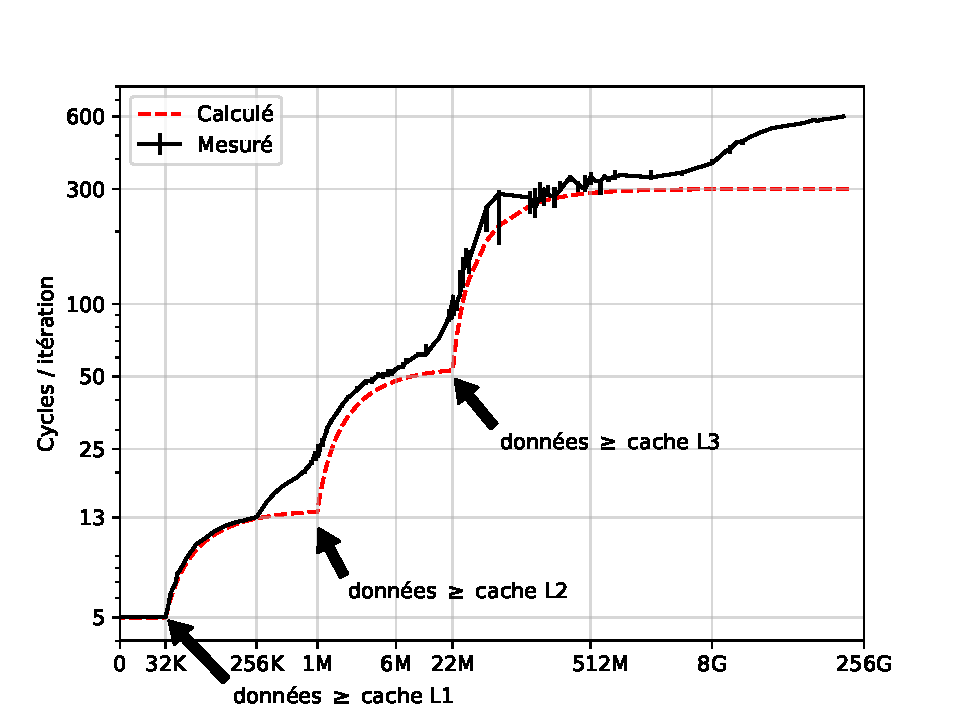
\includegraphics[width=\textwidth]{cache_curve_gr20_w_proba.pdf}
\caption{Résultat du \emph{pointer chasing} benchmark sur le \og \anglais{cluster node}\fg (décrit fig.~\ref{fig:arch2}), avec simulation. \label{fig:chasing_gr20_w_proba}}
\end{figure}

On obtient ainsi une approximation raisonnable de la réalité
(cf. fig.~\ref{fig:chasing_gr20_w_proba}).

 \begin{ddanger}
   La théorie correspond mal à la réalité à partir de 256K. Les latences
   observées sont supérieures à celles qui sont prévues. De plus, le modèle
   simplifié ci-dessus n'explique pas le quasi-doublement de la latence à partir
   de 1G. En fait, ceci résulte d'un \emph{autre} phénomène (qu'on va discuter
   plus tard) : les fautes de TLB et les \og \anglais{page walks}\fg.
 \end{ddanger}

\subsection{Organisation des caches}
\label{sec:cache_line}

Une \emph{ligne de cache} est un bloc de mémoire de taille $B$ dont l'adresse
est un multiple de $B$ (le plus souvent, $B=64$ octets, en tout cas c'est le cas
sur tous les processeurs cités). Le cache stocke en réalité des \emph{lignes de
  cache}, c'est-à-dire des blocs de 64 octets consécutifs en RAM. Ainsi, les
caches L1 de 32Ko stockent généralement 512 lignes de 64 octets. Lorsqu'une
faute de cache a lieu, c'est que l'adresse demandée n'appartient pas à une des
lignes contenues dans le cache. Dans ce cas-là, une des lignes présente dans le
cache est évincée (\emph{evicted}) pour faire de la place, puis la ligne
contenant l'adresse demandée (qui a causé la faute) est lue depuis l'étage du
dessus et elle est stockée toute entière.

Ainsi, une faute de cache sur un mot de 32 ou 64 bits entraine le transfert de
512 bits vers le cache ! C'est notamment pour cette raison que les DIMMs de DDR3
et DDR4 transfèrent les données par paquets de 64 octets : c'est la taille d'une
ligne de cache.

Par ailleurs, un cache de taille $N$ avec des lignes de taille $B$ est capable
de gérer $\leq N/B$ emplacements arbitrairement différents de la mémoire... mais
pas plus.

Lorsqu'une faute de cache a lieu, une ligne actuellement présente dans le cache
doit être évincée afin de faire de la place pour la ligne entrante. Mais
laquelle évincer ? Plusieurs \og politiques de remplacement\fg sont possibles ;
la plus commune consiste sans doute à évincer la ligne de cache qui a été \og
touchée\fg pour la dernière fois il y a le plus longtemps. Cette stratégie
gloutonne (\anglais{Least Recently Used} --- LRU) possède une garantie : on peut
démontrer qu'elle conduit dans le pire des cas à seulement deux fois plus de
fautes de cache que le choix optimal (qu'on ne peut faire qu'en connaissant les
requêtes à venir, ce qui n'est pas le cas de la stratégie LRU).

Une variante largement utilisée (dans tous les caches L1 des processeurs
commerciaux habituels) se nomme PLRU (\anglais{Pseudo-LRU}) : elle consiste à
utiliser une approximation de l'âge de dernier accès à chaque ligne de cache,
plutôt qu'une valeur exacte. Elle est légèrement moins précise mais moins
coûteuse en hardware.

\subsection{Études de cas simples}

\paragraph{Recopie d'un tableau 2D} Considérons une procédure très simple qui
recopie un tableau à deux dimensions. Du point de vue du cache et de la localité
des données, il y a une \og bonne\fg manière de faire et une \og mauvaise\fg
manière de faire.

\medskip

\begin{minipage}{0.49\textwidth}
\begin{minted}{C}
/* Mauvais */
for (int i = 0; i < N; i++)
    for (int j = 0; j <N; j++)
        dst[j][i] = src[j][i];
\end{minted}
\end{minipage}%
\begin{minipage}{0.49\textwidth}
\begin{minted}{C}
/* Bon */
for (int i = 0; i < N; i++)
    for (int j = 0; j < N; j++)
        dst[i][j] = src[i][j];
\end{minted}
\end{minipage}

\medskip

Le mauvais code effectue des accès en mémoire non-contigus. En effet, le langage
C spécifie explicitement le placement en mémoire des tableaux
multi-dimensionnels, et c'est \anglais{row-major} (contrairement à Fortran,
Matlab, R, Julia, ...). Avec une déclaration comme \mintinline{C}{double
  A[N][M];} on trouve que \mintinline{C}{A[i][j]} se trouve en mémoire à
l'adresse \mintinline{C}{A + i*M + j}. Les adresses varient de 1 lorsque le
dernier indice varie, mais de $M$ lorsque le premier indice varie.

Par conséquent, dès que $N \geq 8$, alors chaque accès à
\mintinline{C}{src[j][i]} ou \mintinline{C}{dst[j][i]} est un accès à une ligne
de cache différente (on bouge d'au moins 64 octets lorsque $j$ augmente de
1). Et du coup, lorsque $N > 512$, chaque accès à l'un des deux tableaux
provoque une faute de cache L1 (si le cache L1 fait 32Ko, ce qui courant) avec
la politique de remplacement LRU.

A contrario, le \og bon\fg code lit et écrit les données de manière contiguë,
donc chaque fois qu'une faute de cache a lieu, on a la certitude que les 7
prochains accès seront servis depuis le cache.

Bilan : lorsque $N$ est suffisamment grand, le mauvais code fait $N^2$ fautes de
cache tandis que le bon en fait $\leq N^2 / 8$.

\paragraph{Produit de matrices naïf}

On considère le code suivant, qui effectue le produit de matrice
$C \gets A\times B$. En fait, il pose une variante du problème précédent.
\begin{minted}{C}
for (int i = 0; i < N; i++)
        for (int j = 0; j < N; j++) {
                double x = 0;
                for (int k = 0; k < N; k++)
                        x += A[i * N + k] * B[k * N + j]
                C[i * N + j] = x;
        }
\end{minted}

% \begin{ddanger}
%   On peut espérer que le compilateur soit suffisamment intelligent pour
%   supprimer les deux multiplications entières \texttt{i * N} et \texttt{k * N}
%   ainsi que les additions qui vont avec; mais si on a un doute, on peut les enlever
%   soi-même :
%   \begin{myfilet}
% \begin{minted}{C}
%  for (int i = 0, iN = 0; i < N; i++, iN += N) {
%          double *Ai = A + iN;
%          for (int j = 0; j < N; j++) {
%                  double x = 0;
%                  double *Bj = B + j;
%                  for (int k = 0, kK = 0; k < N; k++, kN += N)
%                          x += Ai[k] * Bj[kN];
%                  C[iN + j] = x;
%          }
%  }
% \end{minted}
%   \end{myfilet}
% \end{ddanger}

Dans ce code, les coefficients de la $i$-ème ligne de $A$ sont tous lus, dans
l'ordre, $N$ fois consécutives (pour chaque~$j$). Même s'ils ne tiennent pas
tous dans le cache L1, alors une faute de cache sur \mintinline{C}{A[i * N + k]}
va charger dans le cache une ligne de cache contenant les 8 prochains
coefficients de la $i$-ème ligne de $A$, donc il n'y aura pas de faute de cache
sur $A$ pendant les 7 prochaines itérations.

Le cas de $B$ est beaucoup plus pénible : $B$ est lu par colonne, et il y a $N$
coefficients de distance entre deux coefficients de $B$ lus de manière
consécutive. Par conséquents, dès que $N \geq 8$, les coefficients de $B$
appartiennent à des lignes de cache différentes. Et dès que $N \geq 512$, alors
un cache L1 standard de 32Ko n'a pas assez de lignes de cache pour stocker une
colonne entière de $B$. Par conséquent, \emph{chaque accès à $B$ provoque alors
  une faute de cache L1} avec la politique de remplacement LRU.

Le produit matriciel naïf est donc une \emph{très} mauvaise idée. En fait, ce
serait bien mieux de calculer d'abord de $B' \gets B^t$ (la transposée de $B$)
puis d'effectuer le calcul $C \gets A \times {B'}^t$ pour éviter ce problème (et
pouvoir lire $B'$ ligne par ligne sans causer de faute de cache systématique)
--- ceci aurait en outre l'avantage de permettre une forme intéressante de
vectorisation.

Le problème, c'est que calculer la transposée prend du temps, et que ça risque
d'en faire perdre plus que ça n'en fait gagner. Pour de petites valeurs de $N$,
ça ne vaudra sûrement pas le coup. Mais pour $N=3200$, par exemple, la
combinaison \og transposée + produit avec la transposée\fg met 63s ($0.25$ faute
L1 / itération), tandis que le produit direct met 177s (une faute L1 /
itération). On y gagne donc vraiment.

\section{Caches : considérations avancées}

\subsection{Écritures dans les cache} Les écritures peuvent elles aussi causer
des fautes de cache, mais là plusieurs solutions sont possibles. Dans tous les
cas, si l'adresse écrite appartient à une ligne présente dans le cache, alors le
cache est mis à jour. C'est ce qui se passe ensuite qui peut varier.

La première solution (\og \emph{write-through}) consiste à relayer
systématiquement les opérations d'écriture à l'étage du dessus. Si une écriture
concerne une adresse qui n'est pas dans le cache, alors on ne fait rien d'autre.
C'est ce qui se passe dans le PowerPC A2. Avantages : les lignes de cache
peuvent être évincées sans précautions particulières; des écritures vers des
adresses qui vont être abandonnées ne provoquent pas le chargement dans le cache
de lignes inutiles. Inconvénient : les étages supérieurs reçoivent toutes les
écritures.

La deuxième solution (\og \emph{write-back}) consiste à ne pas relayer les
écritures aux étages du dessus en temps réel. Lorsqu'une ligne présente dans le
cache est modifiée, elle est marquée comme \og sale\fg
(\emph{dirty}). Lorsqu'une ligne de cache est évincée, elle est transmise aux
étages du-dessus si et seulement si elle est sale. Si le cache reçoit une
opération d'écriture pour une adresse qu'il ne contient pas, alors cela
déclenche une faute : la ligne en question est d'abord chargée dans le cache
depuis les étages du dessus, puis modifiée et marquée comme sale. Cette
stratégie est la plus répandue. Avantages : des écritures pour des adresses
consécutives sont gérées localement et non transmises au-dessus. Inconvénients :
si on écrit une adresse qu'on ne lit plus jamais après, alors a) 512 bits sont
lus, puis 512 bits sont écrits dans le niveau du dessus et b) l'écriture \og
polue\fg le cache.

\begin{danger}
  Dans le cas d'un cache \og habituel\fg (\anglais{write-back}), une
  optimisation est possible. Quand on \emph{sait} qu'on écrit des données qu'on
  ne va pas chercher à lire bientôt, alors plutôt que de faire une écriture qui
  va polluer le cache avec des choses inutiles, on peut utiliser des
  instructions spéciales d'écriture ou de lecture dites \og
  non-temporelles\fg. Ce sont des instructions de type \texttt{load/store}, mais
  qui permettent de contourner tout ou partie de la hiérarchie des caches. Sur
  les processeurs \textsf{x86}, le jeu d'instruction \textsf{AVX} contient des
  instructions d'écriture non-temporelle (sur 256 bits à la fois) ; son
  extension \textsf{AVX2} contient en outre une instructions de lecture
  non-temporelle (sur 256 bits à la fois).
\end{danger}

\subsection{Problème du \og \anglais{False Sharing}\fg} L'explication donnée
ci-dessus sur les politiques d'écriture dans les caches néglige un détail dans
le cas des machines multi-coeurs. En effet, la plupart (mais il y a des
exceptions...)  maintiennent la \emph{cohérence des caches}. Le problème est le
suivant : un thread matériel écrit une valeur en RAM alors que d'autres unités
d'exécution possèdent la même adresse dans leurs caches. Lorsque l'écriture en
RAM a lieu, les caches des autres processeurs ne reflètent plus la bonne valeur
en mémoire. Pour éviter cette situation, plusieurs solutions sont possibles ;
l'une des plus commune consiste à instaurer un protocole de communication entre
toutes les unités d'exécution : lorsque l'une d'entre elle effectue une
écriture, elle publie l'adresse où l'écriture a eu lieu ; tous les autres
processeurs éjectent de leur cache la ligne qui contenait cette adresse si elle
était présente (en effet son contenu est maintenant périmé). On parle alors
d\emph{invalidation} de la ligne de cache (en effet, elle n'est pas \og
éjectée\fg mais marquée comme \og invalide\fg).

Ce protocole de maintien de la cohérence de cache a un coût, surtout sur les
machines SMP, où des coeurs placés sur des processeurs physiquement distincts
doivent communiquer sur une distance plus grande.

Une conséquence de cette politique de cohérence de cache, c'est que même si deux
threads matériels accèdent à des adresses en mémoire disjointes (pas de
conflit), ils peuvent malgré mutuellement invalider leur cache respectif de
manière répétée s'ils écrivent tous les deux des données qui correspondent à la
même ligne de cache. On parle alors de \og \anglais{False Sharing}\fg : ils ne
partagent pas de données, mais ils partagent une ligne de cache.

Voici un petit programme qui illustre ce problème. 

\begin{minted}{C}
double A[512][8] __attribute__((aligned(64)));
assert(omp_get_max_threads() < 8);
#pragma omp parallel
{                                   /* all threads execute this */
    int k = omp_get_thread_num();
    unsigned int j = 1 + k;         /* different pseudo-random sequence for each thread */
    for (int i = 0; i < 1000000000; i++) {
        A[j % 512][k] *= 3.14; 
        j ^= j << 13;               /* randomize j (XorShift PRNG) */
        j ^= j >> 17;
        j ^= j << 5;
    }
}
\end{minted}

Le tableau A est dimensionné de telle sorte qu'il occupe 32Ko (chaque ligne de
la matrice occupe 64 octets, donc une ligne de cache complète --- en plus on
force le compilateur à aligner le tout sur une adresse qui est un multiple de
64, donc ça commence pile au début d'une ligne de cache). Le tableau tient donc
tout entier dans un cache L1 courant de 32Ko.

Le thread $t$ accède à $A[j][t]$ pour des valeurs arbitraires de $j$. Les
écritures des threads ne sont donc pas conflictuelles (pas besoin de
\texttt{\#omp atomic} ni de synchronisation). Les différents threads ont des
séquences d'indices $j$ différentes. Mais on assiste à un phénomène de
\anglais{False Sharing} : une valeur de $j$ est associée à une seule ligne de
cache, donc chaque fois qu'un coeur traite une valeur de $j$ donnée, ça invalide
la ligne de cache correspondante chez tous les autres. La
figure~\ref{fig:false-sharing} démontre que ça a un effet catastrophique sur les
performances.

\begin{figure}
\begin{center}
\begin{tabular}{|c|c|c|c|c|}
  \hline
  \multirow{2}{*}{\# Coeurs} & \multirow{2}{*}{Temps (s)} & \multicolumn{3}{c|}{Faute de cache / itération / coeur} \\
  \cline{3-5}
                             &           & L1   & L2   & L3 \\
  \hline\hline
  1         &   3.1     & 0.0  & 0.0  & 0.0 \\
\hline
  2         &  20.3     & 1.4  & 2.9  & 0.0 \\
\hline
  4         &  29.9     & 2.1  & 5    & 0.0 \\
\hline
  8         &  52.3     & 2.5  & 7.4  & 0.0 \\
\hline
\end{tabular}
\end{center}
\caption{Résultat de l'exécution du programme qui démontre le \anglais{False
    Sharing} sur le \anglais{cluster node} décrit figure~\ref{fig:arch2}. \label{fig:false-sharing}}
\end{figure}

Avec un seul thread, il n'y a pas de fautes de cache : le tableau $A$ tient tout
entier dans le cache L1 (qui fait 32Ko). Sur la machine où le test a été
réalisé, chaque coeur possède son propre cache L1 et son propre cache L2, tandis
que le cache L3 est partagé. Il n'y a donc pas de \anglais{False Sharing} au
niveau du cache L3. Par contre, on le voit apparaître au niveau du cache L1 et
L2 dès qu'on utilise deux threads ou plus. En effet, chaque écriture par le
thread $t$ provoque l'invalidation de la ligne correspondante du cache L1
\emph{et} du cache L2 de tous les autres coeurs.

Les chiffres précis de la figure~\ref{fig:false-sharing} sont difficiles à
interpréter\footnote{pour l'auteur de ce document en en tout cas...}, mais on
voit bien que le problème s'aggrave avec le nombre de coeurs. Le système qui
mesure le nombre de fautes de cache mesure \emph{plus} d'une faute par
itération, alors qu'il n'y a qu'une lecture/écriture à la même adresse.

\subsection{Associativité}

Un cache de taille $N$ formé de lignes de lignes de taille $B$ possède donc
$N/B$ \og emplacements\fg. Dans l'idéal, il devrait être capable de stocker
n'importe quel bloc de la mémoire dans n'importe lequel de ses
emplacements. S'il en est capable, on dit qu'il est \anglais{fully
  associative}. En réalité, c'est rarement le cas, car cela aurait un coût
matériel prohibitif.

En effet, à chaque accès mémoire, il faut déterminer si l'adresse demandée est
présente dans le cache ou non. Ceci commence par déterminer l'adresse du début
du bloc de RAM (dont l'adresse est un multiple de $B$) qui contient l'adresse
demandée. Ensuite, il faut déterminer si le bloc en question est présent dans le
cache.  Dans un cache \anglais{fully associative}, comme un bloc de mémoire peut
potentiellement être stocké dans n'importe lequel des $N/B$ emplacements, il est
\textit{grosso modo} nécessaire de tous les examiner. C'est donc coûteux,
complexe, énergivore, etc.

À l'autre extrême, on pourrait imaginer un cache simple, qui à chaque bloc de la
mémoire affecte \emph{un} emplacement potentiel. Par exemple, si le cache
contient $2^k$ emplacements, alors il suffit d'extraire $k$ bits de l'adresse du
début du bloc, et ça désigne un des emplacement du cache. L'algorithme qui teste
si un bloc est présent dans le cache est alors particulièrement simple et
efficace : il n'y a qu'un emplacement à tester ! Un tel cache, rudimentaire, est
dit \anglais{direct-mapped}. L'inconvénient de cette stratégie c'est qu'elle
augmente le nombre de fautes de cache, car si deux adresses sont accédées
alternativement et sont \og en compétition\fg pour le même emplacement, alors
chaque accès causera une faute de cache, même s'il est complètement vide par
ailleurs.

Entre le \anglais{direct-mapped} (simple, peu performant) et le
\anglais{fully-associative}, on trouve toute une gamme de compromis avec les
caches \anglais{set-associative}. Dans un tel cache, chaque bloc de RAM peut
être stocké dans un \emph{sous-ensemble} (de taille fixe) des emplacements. Le
cache est découpé en \og \anglais{sets}\fg de petite taille et chaque bloc de
RAM est affecté d'office à un \anglais{set} ; par contre, au sein d'un
\anglais{set} il peut occuper n'importe quel emplacement.

Un cache \emph{$k$-associatif} possède des \anglais{sets} de taille~$k$ : il
peut stocker un bloc arbitraire dans seulement $k$ emplacements possibles (sur
les $N/B$). L'avantage, c'est que pour tester si un bloc est présent dans le
cache, il suffit de tester seulement $k$ emplacements possibles. Une des
manières dont ceci peut être réalisé consiste à extraire une partie des bits de
l'adresse du bloc à stocker pour désigner le \anglais{set}.

La quasi-totalité des caches sur les processeurs commerciaux sont
associatifs. La figure~\ref{tab:cache_associativity} donne quelques exemples. Là
encore, on voit qu'il y a beaucoup de variabilité d'une machine à l'autre. La
seule espèce de constante est la taille des lignes de cache fixée à 64 octets.

\begin{figure}
  \centering
  \begin{tabular}{|c|c|c|c|c|}
  \hline
  CPU        & niveau & $N$  & $B$    & Associativité \\
  \hline\hline
    \multirow{2}{*}{Cortex A53} & 1   & 32K    & 64     & 4 \\
                                & 2   & 512K   & 64     & 16 \\
    \hline
    \multirow{2}{*}{PowerPC A2} & 1   & 16K   & 64    & 8 \\
                                & 2   & 32M   & 128   & 16 \\
    \hline
    \multirow{3}{*}{Xeon E5-2695 v4 (Broadwell)}  & 1   & 32K    & 64    & 8  \\
                                                  & 2   & 256K   & 64    & 8  \\
                                                  & 3   & 45M    & 64    & 20  \\
    \hline
    \multirow{3}{*}{Core i7-6600U (Skylake)}      & 1   & 32K    & 64    & 8  \\
                                                  & 2   & 256K   & 64    & 4  \\
                                                  & 3   & 4M     & 64    & 16  \\
    \hline
    \multirow{3}{*}{Xeon Gold 6130 (Skylake)}  & 1   & 32K    & 64    & 8  \\
                                               & 2   & 1M     & 64    & 16  \\
             & 3   & 22M    & 64    & 11  \\
    \hline
  \end{tabular}
\caption{Associativité de quelques caches. \label{tab:cache_associativity}}
\end{figure}

L'associativité des caches pose parfois des problèmes en causant des fautes de
caches inattendues, en particulier quand on travaille avec des tableaux dont la
taille est une puissance de deux. Par exemple, considérons le petit bout de code
suivant, qui transpose (naïvement) une matrice carrée.

\begin{minted}{C}
for (int i = 0; i < N; i++)
    for (int j = 0; j < N; j++)
        B[i * N + j] = A[j * N + i];
\end{minted}

\begin{figure}
\centering
\begin{tabular}{|c|c|c|c|}
  \hline
  $N$ & Temps (ms) & Faute L1 / \texttt{double} (lecture) & Faute L1 / \texttt{double} (écriture) \\ 
  \hline
  31 & 1.3         & 0 & 0 \\
  32 & 1.3         & 0 & 0 \\
  33 & 1.3         & 0 & 0 \\
  \hline
  63 & 3.5         & 0.12 & 0.11 \\
  64 & 3.5         & 0.22 & 0.12 \\
  65 & 4           & 0.11 & 0.10 \\
  \hline
  127 & 8          & 0.13 & 0.12 \\
  128 & 16         & 1    & 0.12 \\
  129 & 9          & 0.23 & 0.12 \\
  \hline
  255 & 36         & 0.13 & 0.11 \\
  256 & 119        & 1    & 0.12 \\
  257 & 37         & 0.14 & 0.11 \\
  \hline
\end{tabular}
\caption{Mise en évidence problèmes d'associativité (transposition naïve). Les
  deux colonnes de droites indiquent le nombre de fautes de cache par
  \texttt{double} copié de $A$ vers $B$ (mesure expérimentale). \label{tab:pb-associativity}}
\end{figure}

Si on l'exécute sur de petites valeurs de $N$ (avec les deux matrices qui
tiennent largement dans un cache L2 de 256Ko, par exemple), on observe un
comportement pathologique pour $N=2^7$ et $N= 2^8$, ainsi que le montre la
figure~\ref{tab:pb-associativity}. Lorsque les deux matrices ne tiennent pas
dans le cache L1 (ce qui est le cas dès que $N \geq 46$), on s'attend à ce
qu'une lecture de $A$ (resp. écriture de $B$) sur huit cause une une faute de
cache L1 \texttt{double} : chaque faute aboutit au transfert des 8 prochains
éléments de $A$ (resp. $B$) dans le cache. C'est bien ce qu'on observe
($1/8 = 0.125$).

On voit que ce chiffre est sensiblement dépassé pour les puissances de deux,
puisqu'on a alors une faute de cache par lecture de $A$ ! Le temps d'exécution
est lui aussi sensiblement augmenté. Ceci s'explique par le fait que les
adresses lues (pour $A$) dans deux itérations successives diffèrent d'une
puissance de deux (suffisamment grande). Dans le cas de ce cache L1 de 32Ko avec
des lignes de $B=64$, on peut parier que le \anglais{set} d'un bloc de RAM
contenant une adresse $x$ est déterminé en prenant les bits $[6:12]$ de
l'écriture de $x$ en binaire.

Supposons que c'est vrai : ceci impliquerait que deux adresses distantes de
$k \cdot 2^{12}$ octets tombent forcément dans le même \emph{set} (pour
n'importe quel $k$), qui ne contient que 8 emplacements. Donc, avec $N=64$, lors
d'un tour de la boucle externe, les adresses lues dans $A$
($8 \times 64j + 8i$) ne sont pas contiguës, et elles appartiennent
toutes à des lignes de cache différentes. Or, ces lignes de cache ne peuvent
tomber que dans un sous-ensemble de 8 \anglais{sets} sur 64 (par exemple, pour
$i=0$ : $0, 8, 16, \dots, 48, 56$).

En tout état de cause, 64 lignes de cache à répartir dans 8 sets de capacité 8,
ça peut tenir, mais tout juste !  En pratique on observe un début de dégradation
des performances pour $N=64$. Par contre, à partir de $N=128$, ça craque : les
lignes transférées vers le cache L1 pour servir les lectures de $A$ ne peuvent
atterrir que dans 4 \anglais{sets} : le nombre total d'emplacements disponibles
n'est plus alors que de 32, alors qu'il en faudrait 128. En pratique, chaque
nouvelle lecture de $A$ provoque une faute.

Le programme le plus simple qui exhibe le comportement problématique est le
suivant :
\begin{minted}{C}
double A[4608];
...
double x = 0;
for (int k = 0; k < N; k++)
    for (int i = 0; i < 9; i++)
        x += A[512 * i];
\end{minted}
Avec un cache $8$-associatif, il effectue une faute de cache par itération de la
boucle externe, alors qu'il n'accède qu'à 9 adresses différentes, pour un total
de 72 octets !




\clearpage

\section{Aspects théoriques}

\subsection{Modèle IO}

\subsection{Algorithmes \og \anglais{Cache-Oblivious}}

Algo cache-oblivious ?


\section{Hiérarchie mémoire : le TLB et la pagination}

Sur la figure~\ref{fig:chasing_pi} (raspberry Pi \texttt{3B+}), les caches
expliquent entièrement la forme de la courbe jusqu'à $N=128$Mo, mais ne
justifient pas le quasi-doublement de la latence de 128Mo à 800Mo. En fait, un
\emph{autre} phénomène intervient.

\paragraph{Mécanisme de pagination}

Les processeurs (et les systèmes d'exploitation) modernent distinguent deux
types d'adresses mémoires : les adresses \emph{virtuelles} et les adresses
\emph{physiques}. Les adresses physiques sont celles qui sont comprises par le
matériel (contrôleur mémoire, barrettes de RAM, etc.).

Les programmes \og normaux\fg ne manipulent que des adresses
virtuelles. D'ailleurs, dans les systèmes d'exploitations multi-tâches modernes,
chaque processus a l'illusion de s'exécuter dans un espace mémoire virtuel qui
lui est propre : sur une machine 32-bits (resp. 64 bits), tout se passe comme si
chaque processus avait toute une mémoire de $2^{32}$ octets (resp. $2^{64}$) à
sa disposition. Ceci permet notamment de garantir l'isolation des processus les
uns par rapports aux autres.

Les instructions exécutées par le CPU pour le compte des programme utilisateur
manipulent donc des adresses logiques; mais au bout d'un moment, il faut bien
accéder à la RAM, donc un mécanisme de conversion \og logique $\leftrightarrow$
physique\fg doit bien être mis en oeuvre : c'est le rôle du MMU (\emph{Memory
  Management Unit}).

Pour gérer cette correspondance, la quasi-totalité des architectures qui
utilisent des adresses logiques mettent en oeuvre un système de
\emph{pagination} de la mémoire : l'espace mémoire virtuel est divisé en
\emph{pages}. Une page est une plage d'adresses contigüe de taille $k$, dont
l'adresse (virtuelle) est un multiple de $k$. De manière classique, on a
$k=4$Ko. Généralement, les bits de poids faible de l'adresse virtuelle (qui
indiquent la position à l'intérieur de la page) coïncident avec ceux de
l'adresse physique.

Le système d'exploitation stocke, pour chaque page, plusieurs informations, et
en premier lieu l'adresse physique correspondante. De manière additionnelle,
l'OS stocke aussi quelques bits pratiques : la page est-elle présente en RAM (si
non, c'est qu'elle a été stockée dans le fichier d'échange pour libérer de
l'espace) ? Le processus en cours a-t-il le droit de lire/d'écrire la page en
question (sinon, c'est la fameuse \og erreur de segmentation\fg) ? etc.

Outre l'isolation des processus les uns des autres, la pagination sert aussi et
surtout à permettre la mise en oeuvre de la \og mémoire virtuelle\fg
(c.a.d. l'extension de la RAM par un périphérique de stockage). La pagination
permet enfin de partager de manière sélective des zones de mémoire entre des
processus différents, ou de mettre en place l'appel système \texttt{fork} et son
mécanisme de \og \emph{copy-on-write}\fg, etc. etc. etc.

La pagination nécessite donc une coopération entre l'OS et le MMU. Sur la
plupart des architectures, ceci se passe de la façon suivante : une instruction
privilégiée du CPU permet à l'OS d'indiquer au MMU l'adresse (physique) d'une
\emph{table des pages}. Les détails concrets peuvent varier d'une archiecture à
l'autre, alors voici comment ça se passe sur les processeurs \texttt{x86-64}, en
mode 64 bits : le registre \texttt{cr3} du CPU contient l'adresse (physique)
d'une table des pages de niveau 4. Celle-ci contient 512 pointeurs (physiques)
vers des tables de page de niveau 3, qui contiennent elles-même 512 pointeurs
(physiques) vers des tables de page de niveau 2, ..., et enfin les tables de
page de niveau 1 contiennent les informations sur les \og vraies\fg pages (en
fait tout ceci est un arbre d'arité 512 et de hauteur 4).

{\footnotesize Sur le Raspberry Pi \texttt{3B+}, en mode 32-bits, il n'y a que
  deux niveaux de tables; la table de niveau 1 (de taille 16Ko) contient 4096
  entrées de 4 octets, et chaque table de niveau 2 (de taille 1Ko) en contient
  256. Ceci suffit à décrire 1048576 pages de 4Ko, donc 4Go de RAM --- le
  maximum adressable avec des pointeurs 32 bits. Mais le noyau Linux \og
  triche\fg : il n'utilise que 2048 entrées de 8 octets dans la table de niveau
  1, et se débrouille pour tasser 512 entrées dans les tables de niveau 2, qui
  font donc 2Ko...}


Pour convertir une adresse virtuelle $v$ en adresse physique, le processus,
nommé \og \emph{page walk}, est le suivant (résumé par la figure~\ref{fig:paging})~:
\begin{enumerate}
\item Initialiser $x \gets \texttt{cr3}$ ($x$ pointe vers la table de niveau 4).
  \item Pour $i = 4, 3, 2, 1$, faire :
  \begin{enumerate}
  \item Lire les bits $[3+9i:12+9i]$ de $v$ et les stocker dans $j$.
  \item Lire la $j$-ème entrée de la table (de niveau $i$) pointée par $x$, et la stocker dans $x$.
  \end{enumerate}
\item Ici, $x$ contient l'adresse d'un descripteur de page, qui contient
  l'adresse physique de la page.
\end{enumerate}

\begin{figure}
  \centering
  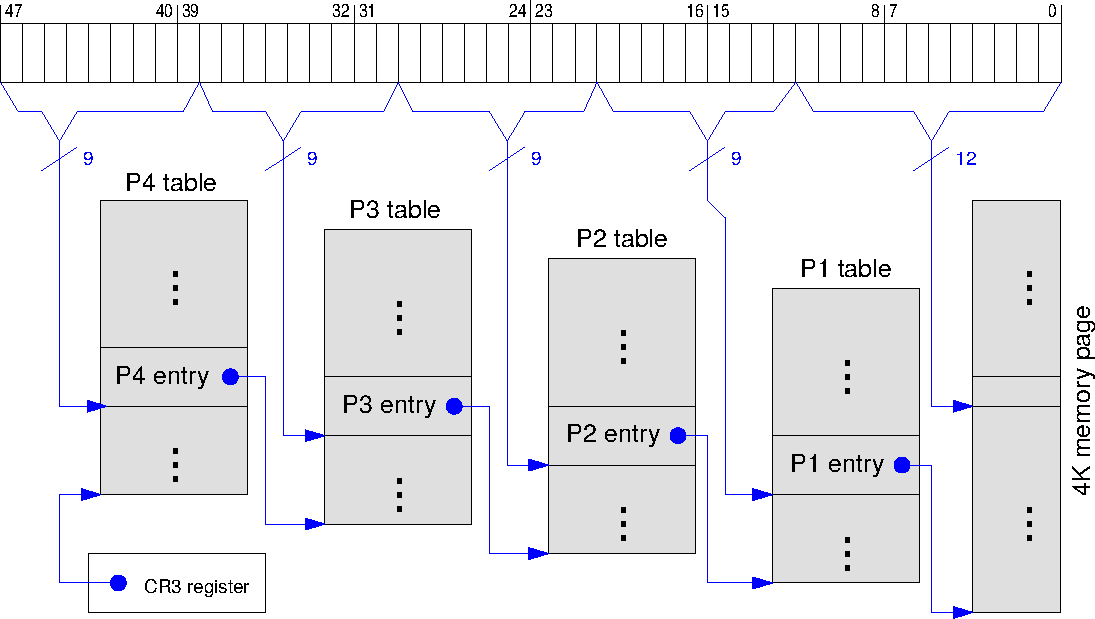
\includegraphics[width=0.5\textwidth]{X86_Paging_64bit.pdf}
  \caption{Correspondance entre adresse virtuelle et indices dans les tables de
    page sur CPU \texttt{x86-64} (image :
    \url{https://os.phil-opp.com/page-tables/}). \label{fig:paging}}
\end{figure}

Sur les processeurs habituels, cette procédre de \emph{page walk} est exécutée
directement par le MMU (dans le processeur), sans intervention du système
d'exploitation. Le \emph{page walk} nécessite 4 accès à la mémoire, et il peut
avoir lieu... lors de n'importe quel accès à la mémoire !

\paragraph{Le \emph{Translation Lookaside Buffer} (TLB)} Pour éviter cette
catastrophe qui multiplierait la latence de tous les accès à la mémoire par 4,
et diviserait le débit de la mémoire par 4, le MMU intègre un cache dédié à la
conversion d'adresses virtuelles en adresses physiques, le TLB. Ce cache
contient l'adresse physique des pages accédées recemment, et sa taille varie de
512 entrées (Raspberry Pi) jusqu'à 1536 entrées (processeurs Intel récents, à
partir de la génération \og SkyLake\fg). Si, lors de la conversion d'une adresse
virtuelle en adresse physique, la page correspondante est présente dans le TLB,
il y a un \og \emph{TLB hit}. Dans le cas contraire, il y a un \emph{TLB miss}
et le \emph{page walk} est déclenché.

Le \emph{page walk} n'a donc jamais lieu si les données avec lesquelles on
travaille occupent moins de $\{512, 1024, 1536\}$ pages, donc si elles sont de
taille inférieure à
$[\# \text{entrées du TLB}] \times [\text{taille d'une page}]$, soit 2, 4 ou
6Mo.

\begin{danger}
  En fait, c'est encore plus compliqué que ça. Les processeurs Intel
  contemporains n'ont pas \emph{un} TLB, mais \emph{deux} TLBs, un de niveau 1
  (petit et rapide) plus un de niveau 2 (plus gros, plus lent). La taille donnée
  ci-dessus (1536 entrées) est la taille du TLB2. Le TLB1 est de taille 32 ou
  64.
\end{danger}

\paragraph{Espace occupé par les tables de pages} Sur les processeurs
\texttt{x86-64}, pour pouvoir adresser $N$ octets de RAM, il faut $N / 4096$
pages, donc $N / (4096 \times 512)$ tables de pages de niveau 1. Chacune d'entre
elle occupe une page (4096 octets), donc au total ces dernières occupent $N/512$
octets. Ça ne représente pas un espace énorme, mais ce sont des données auquel
le CPU accède régulièrement.

En effet, lorsque le \emph{page walk} a lieu, les tables de page sont lues par
le MMU en passant par la hiérarchie mémoire habituelle, donc par les caches. Et
le problème, c'est que s'il y a beaucoup de fautes de TLB, donc beaucoup de
\emph{page walks}, alors a) les \emph{page walk} vont eux aussi causer des
fautes de cache, si les tables de pages demandées ne sont pas en cache, et par
conséquent b) les tables de page vont évincer les \og vraies\fg données des
caches. Du coup, dans les caches, les \og vraies\fg données cohabitent avec les
tables de page, dans des proportions variables selon le niveau de cache et pas
très faciles à prévoir à l'avance.

% \begin{tabular}{|c|ScSc|}
% \hline
%   Niveau & Espace occupé            & Fréquence d'accès \\
%     \hline  \hline
%   4      & 4096                                     & 1 \\
%   3      & $\max\left(4096, N \cdot 2^{-27}\right)$ & $2^{-27}$ \\
%   2      & $\max\left(4096, N \cdot 2^{-18}\right)$ & $2^{-18}$ \\
%   1      & $\max\left(4096, N \cdot 2^{-9 }\right)$ & $2^{-9}$ \\

%   \hline
% \end{tabular}

Mais en tout cas, on peut observer l'augmentation du nombre de fautes de caches
et/ou de TLB. La librarie \texttt{PAPI} permet d'accéder aux mécanismes de
mesure de performances de manière assez portable sur de nombreuses
plate-formes. Ceci a permis d'instrumenter le code de \emph{pointer chasing}, et
on peut voir les résultats sur la figure~\ref{fig:chasing_pi_misses}.

\begin{figure}
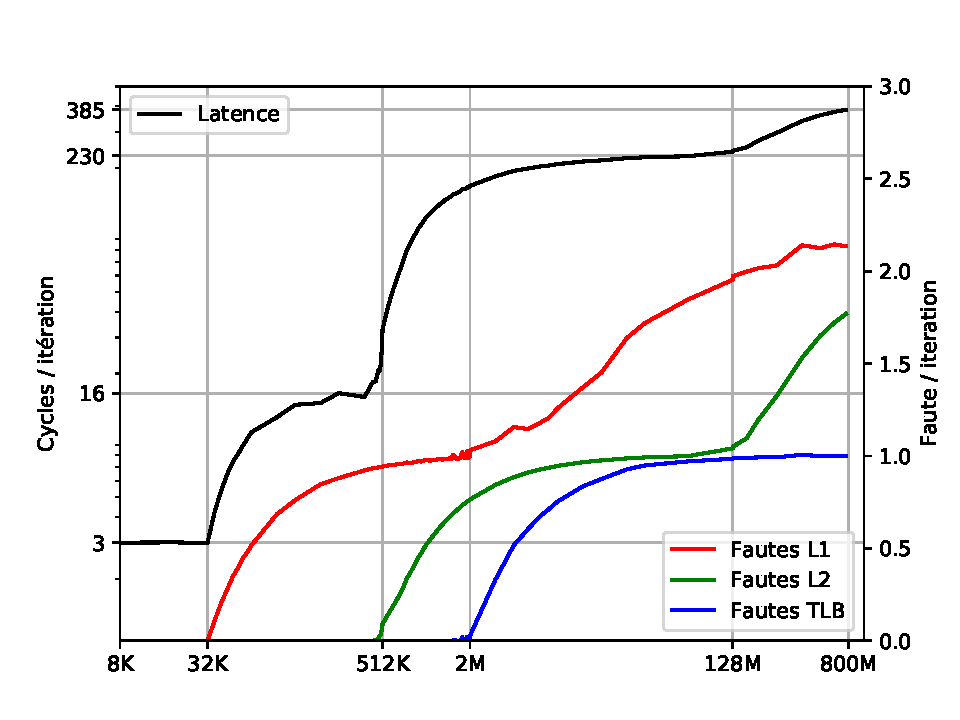
\includegraphics[width=\textwidth]{miss_curve_pi.pdf}
\caption{Fautes de cache et de TLB du \emph{pointer chasing} benchmark sur un
  Raspberry Pi \texttt{3B+}. \label{fig:chasing_pi_misses}}
\end{figure}

Lorsque $2 \geq 2$Mo, les données occupent plus de pages que le TLB n'a
d'entrées, donc on commence à voir apparaître des fautes de TLB. Les \emph{page
  walks} font augmenter le nombre de fautes de cache L1. À partir de
$N \geq 128$Mo, les tables de pages ne tiennent plus dans le cache L1, et les
\emph{page walks} causent des fautes de cache L2. À ce moment-là, chaque
itération de la boucle cause \emph{deux} accès à la mémoire : un pour charger
une entrée d'une table des pages, suivie d'une autre pour charge la valeur
demandée au départ.

\section{Case Study : le \anglais{Bucket Sort}}

\section{Parallélisme des accès mémoire}

Pour accélérer des accès mémoire, la première règle consiste à essayer de faire
tenir les données dans les caches, quite parfois pour cela à modifier les
algorithmes et à faire \emph{plus} de \og calculs\fg.

Si, après ça, la vitesse à laquelle on accède aux données est limitée par la
bande passante de la mémoire, alors il n'y a pas grand-chose à faire. Par
contre, si le problème est la latence de la mémoire, alors on peut
éventuellement gagner quelque chose en exploitant le fait que les processeurs
modernes offrent un certain degré de parallelisme dans les accès à la mémoire :
ils sont capable de gérer plusieurs accès à la mémoire en même temps.

\begin{danger}
  Pendant les années 1990, les processeurs ont évolué : ils ont gagné la
  capacité de supporter plus qu'\emph{une seule} \og \anglais{outstanding cache
    miss}\fg, et c'est monté à 4 environ.  Un \marque{AMD Opteron} de première
  génération de 2005 pouvait gérer 8 fautes de cache simultanément, mais 5-6
  pouvaient saturer l'interface à la RAM.  Pour l'instant, chaque coeur récent
  supporte 10 fautes de cache L1 simultanément. Ca va peut-être augmenter à 12 avec
  les \marque{Intel CannonLake}.  Les \marque{Apple A12 (ARM)} qu'on trouve dans
  les \marque{Iphone X} supportent 40 requêtes simultanées.
\end{danger}

On peut observer et quantifier ce phénomène assez simplement, avec une
modification du \anglais{pointer-chasing benchmark}. Pour mesurer la capacité du
matériel à effectuer plusieurs accès mémoire en parallèle, on peut observer le
temps d'exécution du programme suivant, qui effectue plusieurs fois le
\anglais{pointer chasing} en même temps (avec $n$ \og flux\fg) :
\begin{myfilet}
\begin{minted}{C}
int x0 = 0;
int x1 = 1;
...
int xn = n;
for (int i = 1000000000; i != 0; i--) {
	x0 = T[x0];
	x1 = T[x1];
        ...
	xn = T[xn];
}
\end{minted}
\end{myfilet}

\begin{figure}
  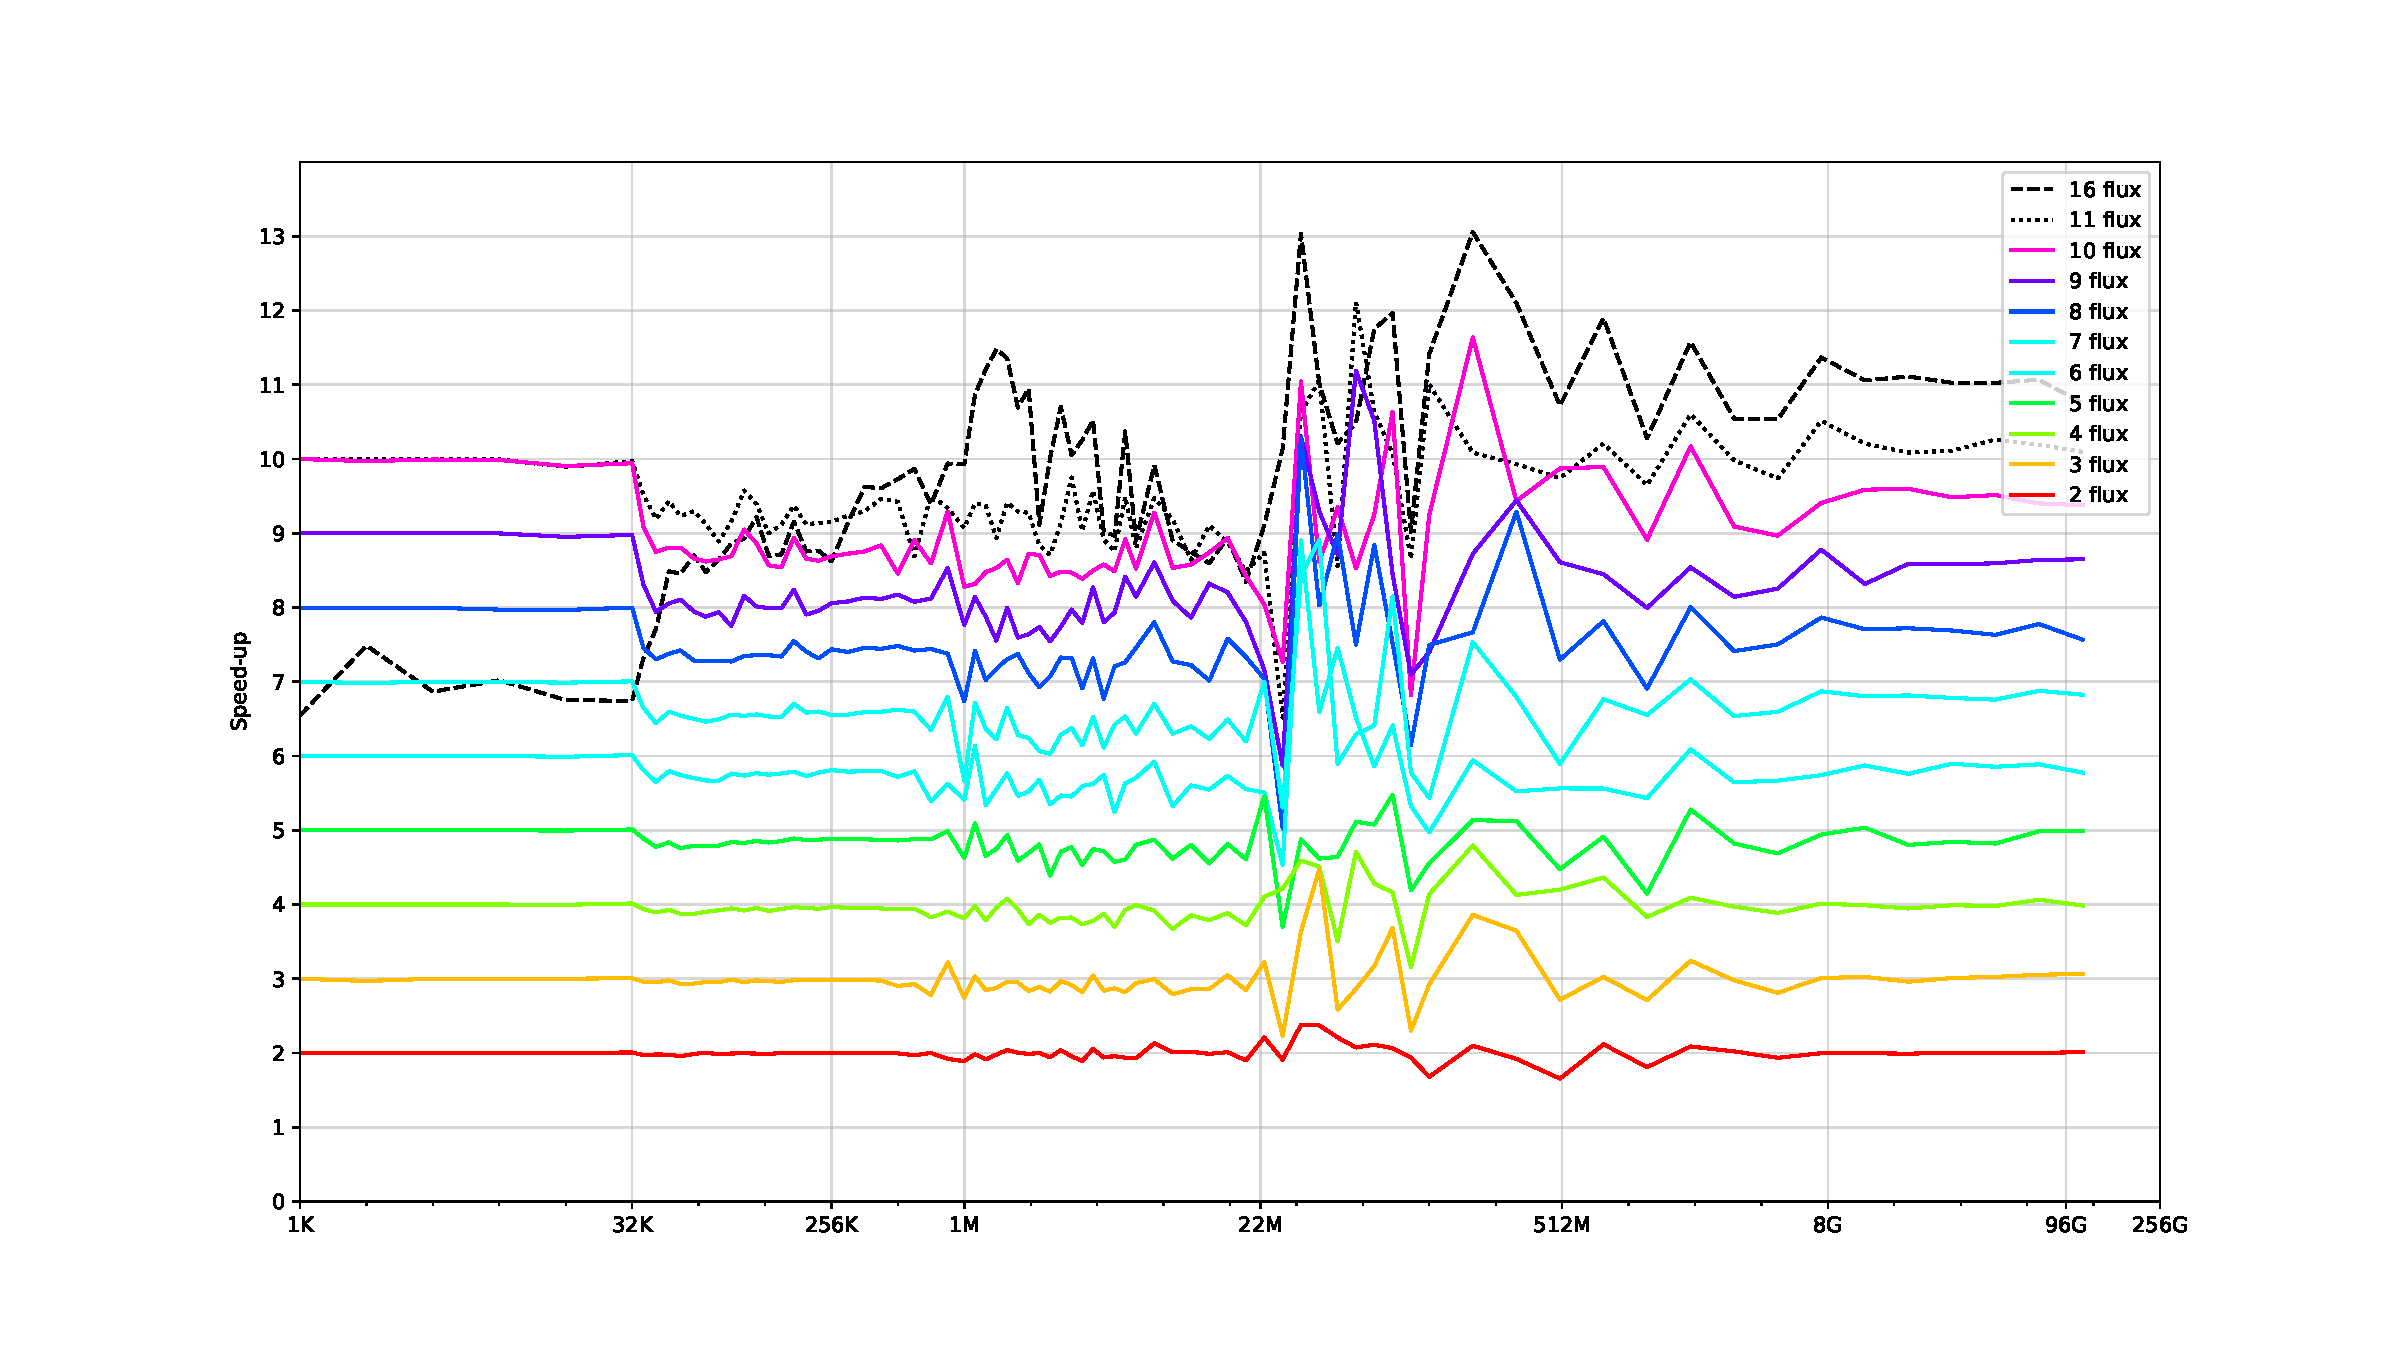
\includegraphics[width=\textwidth]{lane_curve.pdf}
  \caption{Accélération obtenue en suivant plusieurs \og flux\fg simultanés dans
    le \anglais{pointer-chasing} benchmark. L'accélération avec $i$ flux est
    calculée de la façon suivante : c'est $i$ fois la latence mesurée avec
    \emph{un} flux divisée par la latence mesurée avec $i$ flux. Les \emph{huge
      pages} ont été activées.\label{fig:pc-lanes}}
\end{figure}

Les résultats sont visibles figure~\ref{fig:pc-lanes}. On voit que sur un
processeur récent (\marque{Intel Skylake}) le matériel est capable de gérer
jusqu'à 10 accès concurrents au cache L1. Le 11ème n'apporte plus de gain et
ajouter des accès concurrents fait ensuite augmenter la latence d'accès au cache
L1.

\paragraph{loi de Little} La \og loi de Little\fg est un résultat bien connu de
la théorie des files d'attentes, qu'on peut exposer comme ceci : si des clients
arrivent à un guichet avec un débit moyen $A$ (en clients/heure) et que chaque
client attends un temps moyen $T$ (en heures), alors le nombre moyen de client
dans la file d'attente est $N = AT$.

Dans notre cas, elle permet de quantifier le degré de parallélisme au niveau des
instructions qu'il faudrait atteindre pour que tout se passe bien.

Pour essayer de traduire la loi de Little en termes d'accès mémoire, il faut
imaginer que les \og clients\fg sont les instructions qui font des accès à la
mémoire. Le temps d'attente moyen est la latence de la mémoire (c'est le temps
que met l'instruction à recevoir son résultat, donc à être \og servie\fg). En
régime stationnaire où on essaye d'accéder à la mémoire au maximum, le débit des
instructions est lié au débit de la RAM.

Par conséquent, le nombre d'instructions \og en attente\fg est égal au produit
de la bande passante de la mémoire par la latence de la mémoire. Plus
précisément, entre le moment où on initie une lecture vers la RAM et le moment
où on reçoit le résultat, on aurait pu recevoir entre temps $N = AT$ résultats
(demandés avant) si tout s'était bien passé. Ceci signifie qu'il faut que le
programme puiss \og faire plusieurs choses en même temps\fg pour laisser au
matériel la possibilité d'amortir la latence.

Dans les GPUs, ceci est exploité à grande échelle avec un nombre important de
threads matériels qui exploitent de manière alternée des unités de calculs
lorsque \og leurs\fg données sont prêtes.

\subsection{Case Study : le parcours en largeur}

Considérons un programme (séquentiel) qui effectue un parcours en largeur dans
un gros graphe (creux). Le graphe est représenté par des listes
d'adjacence. Celles-ci sont \og compactées\fg dans un seul tableau d'entiers :
les voisins du sommet $i$ sont \texttt{Ai[Ap[i]: Ap[i + 1]]}, où \texttt{Ap[0] =
  0}, \texttt{Ap[n]} contient le nombre total d'arêtes du graphes. Le nombre de
voisins du sommet $i$ est \texttt{Ap[i + 1] - Ap[i + 1]}. Ceci est trè similaire
aux méthodes habituelles de stockage de représentation en mémoire des matrices
creuses.

Le parcours en largeur fonctionne avec une file. Un sommet est initialement
enfilé. Tant que la file n'est pas vide, on défile un sommet et on enfile ses
enfants.


\section{Et l'énergie dans tout ça ?}

Un CPU ne consomme pas toujours autant d'énergie. Il a une consommation
\emph{statique}, indépendante de l'instruction exécutée et une consommation
\emph{dynamique} qui dépend de ce qu'il est en train de faire.

Voici le résultat des mesures sur un processeur Intel Core i5-2500 (de 2011).

\begin{center}
\begin{tabular}{|c|c||c|c|}
  \hline
  opération & type & instruction / cycle (max) & nJ / instruction \\
  \hline\hline
  $\emptyset$  &           &                & 0.37 (par cycle, par coeur) \\
  \hline
  \verb@+, -, &, |@ &int64 & $\approx 3$    & 1.1  \\
  $\times$               &int64 & 1              & 2.8  \\       
  $\div$               &int64 & 0.025--0.034   & 93--132 \\
  \hline
  $+, -$       & float64 & $\approx 1$    & 3.2 \\
  $\times$            & float64 & $\approx 0.6$  & 4.5 \\
  \hline
  reg $\gets$ reg         & int64 & $\approx 3$    & 1.07 \\
  reg $\gets$ L1 cache    & int64 & $\approx 2$    & 1.8 \\
  reg $\gets$ L2 cache    & int64 & $\approx 1$    & 5 \\
  reg $\gets$ RAM         & int64 & faible         & 20 \\
  L1 $\gets$ reg          & int64 & $\approx 1$    & 3.08 \\
  L2 $\gets$ reg          & int64 & $\approx 1$    & 5--10 \\
  RAM $\gets$ reg         & int64 & faible         & 38.6 \\
  \hline
\end{tabular}
\end{center}

Plusieurs observations sont notables. Les écritures sont deux fois plus lentes
et plus énergivore que les lectures. Les opérations flottantes consomment
environ $3\times$ plus d'énergie que leurs homologues entières. Mais surtout,
déplacer des données entre le CPU et la hiérarchie mémoire consomme plus
d'énergie que presque n'importe quoi d'autre. Et plus les données doivent aller
loin, plus ça consomme. De manière équivalente, déplacer des données vers un
autre processeur, ou vers une autre machine consomme encore bien plus.

Bref, pour a) obtenir de bonnes performances et b) ne pas consommer trop
d'énergie, il faut surtout... ne pas accéder à la mémoire (ou en tout cas, se
limiter aux caches les plus proches).

\chapter{\og Memory Wall\fg, performance de crête et équilibrage}
\label{ch:roofline}

Dans le fond, l'objectif du calcul haute-performance consiste à écrire des
programmes qui atteignent des performances les plus proches possibles du maximum
possible sur les machines parallèles utilisées.

\section{Performance de crête d'une machine}

Quand il s'agit du matériel, on parle de \emph{performance de crête}
(\anglais{Peak performance}), et on l'exprime typiquement en FLOPS
(\anglais{Floating Point OPerations per Second}). Cette grandeur quantifie la
puissance de calcul du matériel. Il s'agit généralement d'un maximum
\emph{théorique}, qui est rarement atteint en utilisation normale.

\paragraph{Sequoia} Il y a des cas où son calcul est relativement simple.

Par exemple, la machine \texttt{sequoia} (IBM, 2012, Lawrence Livermore National
Laboratory). Elle a 98\ 304 noeuds, chacun avec un processeur PowerPC A2 de 16
coeurs à 1.6GHz. Ces processeurs sont simples (in-order, pas superscalaires) et
n'exécutent qu'une seule instruction par cycle dans le meilleur des cas. Chaque
coeur dispose d'une unité vectorielle (\og SIMD\fg) qui opère sur des vecteurs
de quatre flottants double précision ($4 \times 64 = 256$ bits). Celle-ci est
capable d'effectuer une opération \og \anglais{Fused-Multiply Add}\fg (FMA) par
cycle. Chaque coeur peut donc faire 8 FLOP par cycle (4 multiplications et 4
additions), dans le meilleur des mondes. La puissance de crête d'un de ces
processeurs est donc de $1.6 \times 10^9 \times 16 \times 8 = 204.8$
GigaFLOPS. Sur l'ensemble de la machine, cela ferait donc
$98\ 304 \times 204.8 = 20.1$ PetaFlops.

Le même genre de calcul peut à peu près se faire sur une partie importante des
processeurs courants pas trop récents, à ceci près qu'ils sont superscalaires,
et donc qu'ils peuvent éventuellement exécuter \emph{plusieurs} instructions par
cycle (il faut trouver combien).

\paragraph{Jean-Zay} Et il y a des cas où le calcul est franchement plus
compliqué.

Penchons-nous sur \texttt{jean-zay}, la machine récemment acquise par le CNRS
(on ne s'intéresse qu'à la partie CPU, on laisse les GPUs de côté, et c'est déjà
assez compliqué comme ça). Elle dispose de 1528 noeuds possédant deux
processeurs Intel Xeon Gold 6248 (Cascade Lake) de 20 coeurs à 2.5Ghz avec
l'\textsf{AVX512}. Cette unité SIMD est capable de faire des opérations sur 8
flottants en double précision (ou 16 en simple précision).

Première observation, on peut sur le papier faire deux fois plus de FLOPS avec
des \texttt{float} qu'avec des \texttt{double}... Mais on va se limiter aux
\texttt{double} pour l'instant et pour simplifier.

L'\textsf{AVX512} possède une instruction FMA. Les Xeon Scalable d'entrée de
gamme (Bronze et Silver) peuvent faire un FMA 512-bits par cycle, tandis que les
haut de gamme (Gold et Platinum) peuvent en faire deux.

Dans notre cas, on a donc le droit à deux FMA par cycle sur 8 \texttt{double},
donc à 32 FLOP par cycle sur chaque coeur. Et maintenant, les problèmes
commencent. Combien y a-t-il de cycle par seconde ? On nous dit \og 2.5Ghz\fg,
mais en fait c'est plus compliqué que ça. Ces processeurs ont la capacité
d'augmenter la fréquence des coeurs individuellement, tant que la puissance
dissipée n'est pas trop élevée. Commercialement, cela s'appelle le
\anglais{Turbo Boost} : ils sont tous capable de fonctionner ensemble à 2.5Ghz
(fréquence de base normale), mais si un seul est actif il peut aller jusqu'à
3.9Ghz (fréquence turbo normale).

Et en réalité, c'est encore plus compliqué. Si un coeur ne fait que des
opérations scalaires ou vectorielles AVX2 \og légères\fg (pas de flottants ni de
multiplication/division), alors il est en mode \og normal\fg. S'il fait
beaucoup d opérations vectorielles AVX2 lourdes (ou des AVX512 légères), alors il passe
en mode AVX2 et sa fréquence \emph{baisse}. Enfin, s'il fait des opérations
AVX512 lourdes, il passe en mode AVX512 et sa fréquence baisse encore.

Du coup, chaque coeur peut fonctionner à une fréquence différente en fonction du
mode dans lequel il se trouve et de combien d'autres sont actifs. Le
tableau~\ref{tab:freq-scaling-xeon} montre les bornes inférieures et
supérieures. Au passage, on voit qu'en passant d'un code scalaire à un code
AVX512, on gagne plutôt un facteur $5.1$ qu'un facteur 8 (à cause de la
réduction potentielle de la fréquence de 36\%).

\begin{figure}
  \centering
\begin{tabular}{|c|c||c|c|c|c|c|c|c|c|}
  \hline
  \multirow{2}{*}{Mode}   & \multirow{2}{*}{Base} & \multicolumn{6}{c|}{Turbo avec $x$ coeurs actifs} \\
%  \cline{3-23}
  & &             1-2 & 3-4 & 5-8 & 9-12 & 13-16 & 17-20 \\
  \hline\hline
  normal & 2.5	& 3.9 & 3.7 & 3.6 & 3.6 & 3.4 & 3.2 \\
  \hline
  AVX2	 & 1.9	& 3.8 & 3.6 & 3.5 & 3.4 & 3.0 & 2.8 \\
  \hline
  AVX512 & 1.6	& 3.8 & 3.6 & 3.5 & 3.0 & 2.7 & 2.5 \\
  \hline
\end{tabular}
\caption{Fréquence limites pour le Xeon Gold 6248 (Cascade Lake). Chaque coeur
  peut se trouver entre la fréquence de base et la fréquence turbo du mode
  concerné. Ces chiffres varient d'un modèle à
  l'autre. \label{tab:freq-scaling-xeon}}
\end{figure}

Du coup, on sait que quoi qu'il arrive, on peut atteindre 1.6Ghz sur les 20
coeurs à la fois en faisant de l'AVX512. Ceci donnerait
$1.6 \times 10^9 \times 20 \times 32 = 1024$ GFLOPS par processeur, donc
$1528 \times 2 \times 1024 = 3.1$ PFLOPS pour l'ensemble de la machine.

\subsection{Peut-on atteindre la performance de crête ?}

Réponse courte : ça dépend mais probablement pas (malgré des efforts importants). 

En tout cas, sans faire d'efforts, c'est sûr qu'on en sera très très loin ! Le
produit de matrice naïf qui apparaît au début du chapitre~\ref{ch:intro}
atteint péniblement 1.6 GFLOPS sur un noeud de \texttt{jean-zay} capable d'en
faire 2048 \og en crête\fg. On est donc à $0.08\%$ de la puissance de crête
\emph{d'un seul noeud} !

\begin{minted}{C}
/* très mauvais */
for (int i = 0; i < n; i++)
    for (int j = 0; j < n; j++)
        for (int k = 0; k < n; k++)
            C[i][j] += A[i][k] * B[k][j];
\end{minted}

\begin{danger}
  Il faut bien se comprendre : le but est de finir les calculs le plus vite
  possible, pas de faire le plus de FLOPS possible. Si on a un algorithme
  $\mathcal{A}$ (par ex. un solveur linéaire creux) qui termine en 10 minutes en
  faisant peu de FLOPS, il vaut mieux l'utiliser plutôt que l'algorithme
  $\mathcal{B}$ (par ex. un solveur linéaire dense) qui fait plein de FLOPS mais
  qui termine en trois jours...
\end{danger}

Les petits calculs ci-dessus montrent que pour atteindre la performance de crête
d'une machine parallèle, il faut forcément :
\begin{itemize}
\item Utiliser tous les noeuds à 100\% (pas de temps de communication et bon équilibrage de charge).
  
\item Utiliser tous les coeurs à 100\% (pas de surcoût et bon équilibrage de charge).

\item Utiliser la vectorisation, et en particulier utiliser quasi-exclusivement des FMA.

\item Exploiter le parallélisme au niveau des instructions (ILP) pour fournir aux unités d'exécutions deux FMA \og prêts à exécuter\fg par cycle.
\end{itemize}

\medskip

Obtenir de bonnes performances nécessite donc forcément des efforts de
programmation non-triviaux, et/ou l'usage de librairies \og sur étagères\fg
(\anglais{off-the-shelf}) très optimisées.

Mais de toute façon, là-dessus vient se greffer le problème du \anglais{Memory
  Wall} abordé dans le chapitre~\ref{chap:memory}. Si la mémoire n'est pas
capable de fournir les données aux unités d'exécution, alors on n'a aucune
chance de s'approcher de la puissance de crête. Et en réalité, beaucoup de
calculs sont \anglais{memory-bound}, c'est-à-dire limités par la bande passante
de la mémoire.

\section{Modèle \og \anglais{Roofline}\fg}

Généralement, dans le monde du calcul scientifique de pointe, on cherche à
optimiser un petit nombre d'applications pour \emph{une} machine donnée (celle
qu'on a sous la main).

\begin{danger}
  Par exemple, quand le CNRS a fait l'acquisition de \texttt{jean-zay}, le
  fournisseur devait s'engager à porter 6 applications importantes pour la
  communautés des utilisateurs, avec un niveau de performance garanti par
  contrat...
\end{danger}

Quand on est confronté au problème d'optimiser \emph{une} application
particulière sur \emph{une} machine donnée, il faut d'abord connaître les
limites de la machine, mesurer les performances de l'application, puis chercher
à comprendre ce qui peut les limiter. Est-ce que le problème c'est que les
unités arithmétiques n'arrivent pas à faire les FLOP assez vite ? Est-ce la
mémoire qui ne peut pas fournir les données assez vite ?  Est-ce le système de
fichier qui est trop lent ? Etc.

\subsection{Version dépouillée}

Le modèle \og Roofline\fg est une représentation graphique simple qui aide à
comprendre les éventuelles limites aux performance d'une application donnée sur
une machine donnée. Il a été introduit en 2009 par Samuel Williams, Andrew
Waterman, and David Patterson dans \og \anglais{Roofline : an insightful visual
  performance model for multicore architectures}\fg~\cite{WilliamsWP09}.

Le modèle vise spécifiquement à comprendre si on se heurte au \anglais{Memory
  Wall} ou pas ; l'article (dont la lecture est assez facile et recommandée) dit
en effet~:
\begin{quote}
  We believe that for the recent past and foreseeable future, off-chip memory
  bandwidth will often be the constraining resource. Hence, we want a model that
  relates processor performance to off-chip memory traffic.
\end{quote}

Le modèle repose sur la notion d'\emph{intensité opérationnelle} du calcul
effectué, c'est-à-dire le nombre d'opérations effectuées par octet transféré
depuis la RAM (c.a.d. transféré entre le contrôleur mémoire et les barrettes de
RAM, et \emph{non} transféré entre un coeur et la hiérarchie des caches).

l'intensité opérationnelle relie entre elles les performances de l'applications
(en FLOPS) avec la bande passante \og de crête\fg de la mémoire. En effet,
on a assez logiquement~:
\[
  \text{FLOPS} \leq \min \bigl([\text{FLOPS de crête}], [\text{intensité opérationnelle}] \times [\text{bande passante RAM de crête}] \bigr)
\]

%équilibrer mix. crête nécessite FMA, donc autant de x que de +.

Le modèle \anglais{Roofline} représente ceci en deux dimensions
(cf. figure~\ref{fig:roofline-basic})~: l'axe des abscisses représente
l'intensité opérationnelle et l'axe des ordonnées représente le nombre de
FLOPS. Une grosse ligne représente la limite supérieure donnée par la formule
ci-dessus : c'est une caractéristique indépassable de la machine elle-même.
Sur ce graphique, la ligne horizontale représente la performance de crête,
tandis que la ligne oblique représente la limite imposée par la bande passante
de la mémoire. On voit que plus l'intensité opérationnelle est faible, plus les
performances de l'application ont peu de chance d'atteindre le maximum
potentiel. Dans l'autre sens, pour espérer atteindre les performances de crête,
il \emph{faut} avoir une intensité opérationnelle élevée.

\begin{figure}
  \centering
  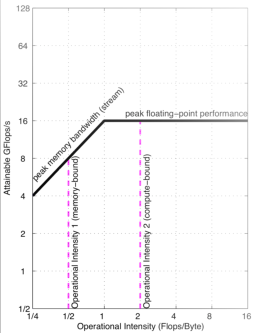
\includegraphics[height=7cm]{roofline_basic.pdf}
  \caption{Un \anglais{Roofline} dépouillé pour une machine fictive avec un seul
    processeur. La performance de crête d'est de 16GigaFLOPS, et la bande
    passante mémoire de 16Go/s. La ligne noire représente le $\min$ de la
    formule.  Les deux lignes pointillées représentent deux applications
    différentes qui ont deux intensités opérationnelles différentes.
    L'application 1 est \anglais{memory-bound}, tandis que l'application 2 est
    \anglais{compute-bound}.  (image:~\cite{WilliamsWP09})\label{fig:roofline-basic}}
\end{figure}

Un premier avantage de ce schéma simple, c'est que cela donne une première idée
de ce qu'on peut attendre d'une application d'intensité opérationnelle donnée
sur une machine donnée.

Des techniques simples permettent parfois d'améliorer un peu l'intensité
opérationnelle, comme la fusion des boucles~:

\smallskip

\begin{minipage}{0.49\textwidth}
\begin{minted}{C}
/* Mauvais */
for (int i = 0; i < N; i++)
    A[i] = B[i] * C[i];
for (int i = 0; i < N; i++)
    D[i] = B[i] + E[i];
\end{minted}
\end{minipage}%
\begin{minipage}{0.49\textwidth}
\begin{minted}{C}
/* Meilleur */
for (int i = 0; i < N; i++) {
    A[i] += B[i] * C[i];
    D[i] += B[i] + E[i];
}
\end{minted}
\end{minipage}

\medskip

Si $N$ est suffisamment grand, les trois tableaux ne tiendront plus dans le
cache et les données vont devoir être chargées depuis la RAM. Chaque itération
des deux boucles du \og mauvais\fg code transfère 3 \texttt{double} de/vers la
RAM et effectue une opérations (IO = 1/24). Par contre, le \og bon\fg code (qui
calcule la même chose) transfère 5 \texttt{double} et effectue 2 opérations (IO
= 1/20). Le truc c'est que $B[i]$ n'a pas besoin d'être rechargé une deuxième
fois. Les compilateurs effectuent parfois cette optimisation automatiquement.

\subsection{Ajout des \og plafonds\fg}

Si on part d'un code peu ou pas optimisé (séquentiel, pas vectorisé, etc.), un
des intérêt des schémas \anglais{Roofline} c'est qu'ils donnent une idée de ce
qu'on pourrait potentiellement gagner en mettant en oeuvre tel ou tel type
d'optimisation.

On peut faire figurer sur le diagramme les limites correspondant à des
optimisations qu'on envisage (passer à la vectorisation, changer les algorithmes
pour améliorer la localité des accès mémoire, etc.). Sur une machine fixée (par
exemple, un coeur de \texttt{jean-zay}), on peut espérer faire 2.5 GFLOPS avec
des opérations scalaires uniquement, mais 7.6 GFLOPS si on fait de la
vectorisation AVX2, 12.8 GFLOPS avec de la vectorisation AVX512, 25.6 GFLOPS si
on utilise des FMA, et enfin 51.2 si on arrive à en faire deux par cycle. Cela
donne différends \og plafonds\fg atteignable selon le niveau d'optimisation
déployé, et on peut les voir sur la figure~\ref{fig:roofline-jz}.

\begin{figure}
  \centering
  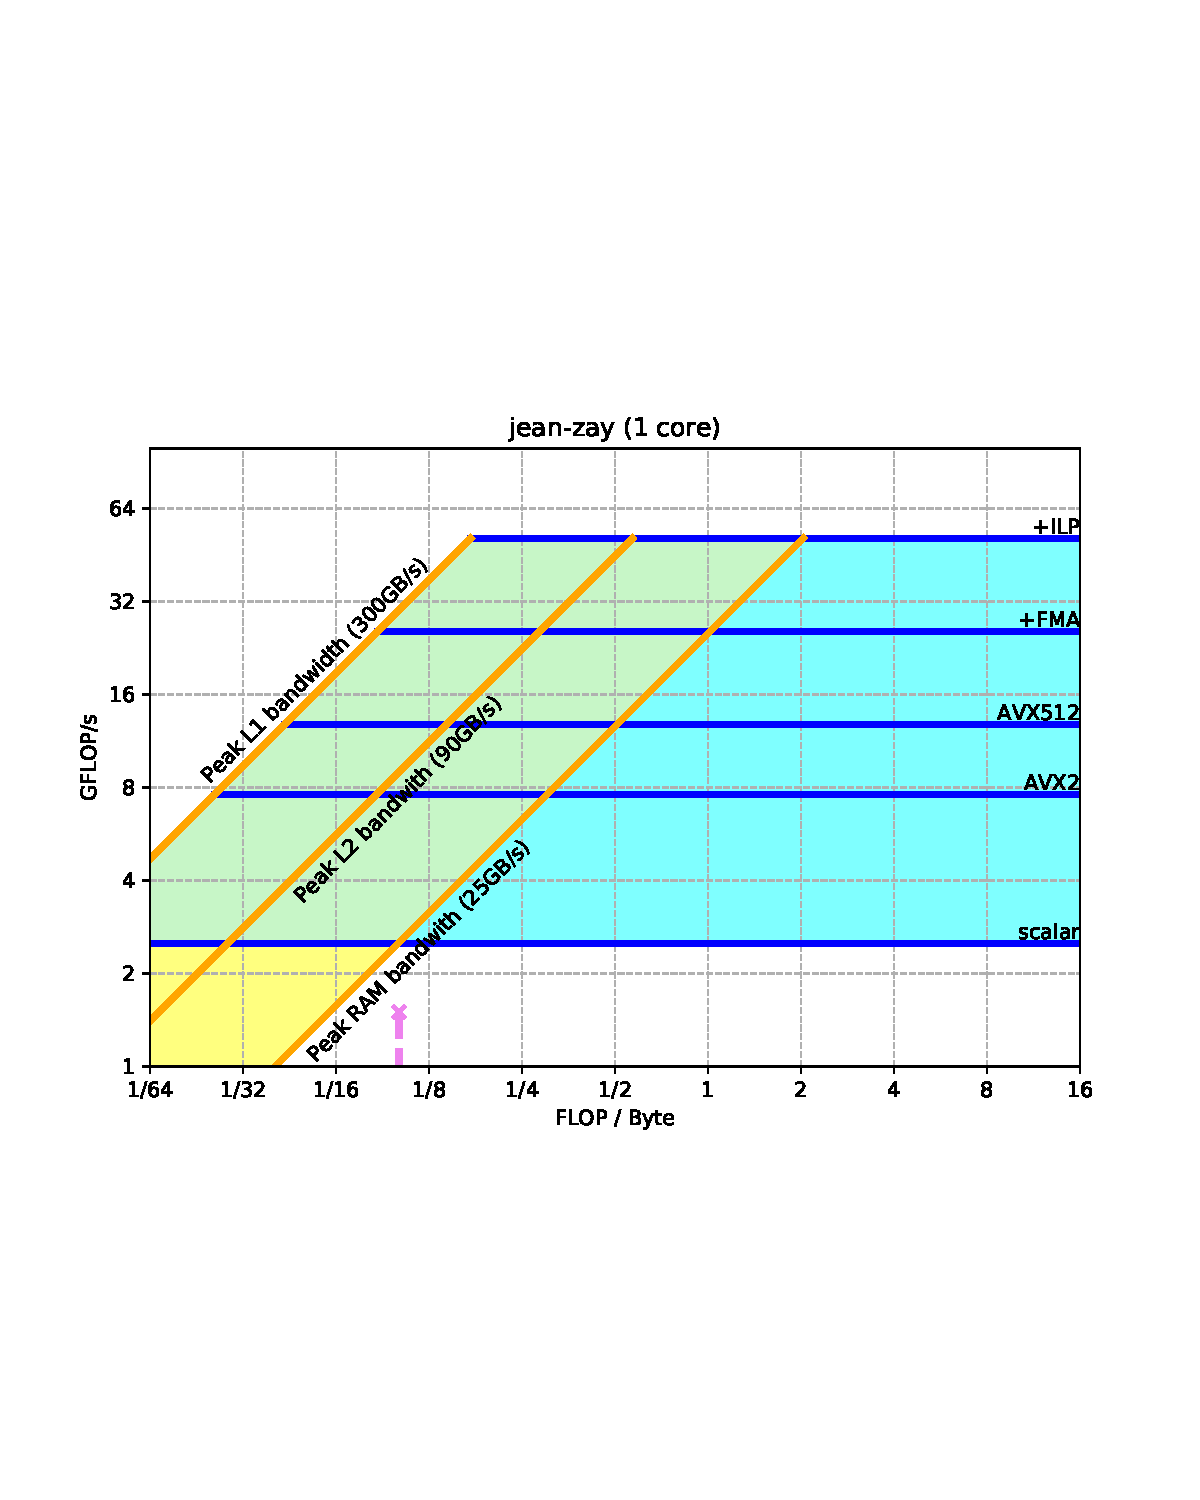
\includegraphics[width=\textwidth]{roofline_jz.pdf}
  \caption{Un schéma \anglais{Roofline} pour un coeur d'un processeur de
    \texttt{jean-zay}. On voit différents \og plafonds\fg. La ligne pointillée
    violette représente les performances obtenues par un code scalaire
    particulier (résolution de $Ax=b$ par la méthode du gradient conjugué).
    \label{fig:roofline-jz}}
\end{figure}

\subsection{Quelques exemples}

\paragraph{Produit scalaire} Prenons un exemple de code de calcul simple : le produit scalaire
\begin{minted}{C}
double res = 0;
for (int j = 0; j < N; j++)
    res += A[i] * B[i];
\end{minted}

Il y a 2 \texttt{double} chargés par itération (16 octets) et deux opérations
arithmétiques. Si les données ne tiennent pas en cache, l'intensité
opérationnelle est donc $1/8$. Si on regarde la droite verticale d'équation
$x=1/8$ sur la figure~\ref{fig:roofline-jz}, on voit que ce petit bout de code
est (probablement) limité par la capacité du CPU à effectuer des opérations
arithmétiques en mode \og scalaire\fg : le plafond \og Peak FLOPS (scalar)\fg
est en dessous de la bande passante de la RAM pour une intensité opérationnelle
de $1/8$. La limite imposée par la bande passante de la RAM est 25.2Go/s
$\times 1/8 = 3.15$ GFLOPS. Si $N$ est grand et que les données ne tiennent pas
en RAM, alors on a intérêt à mettre en oeuvre une forme de vectorisation (par
exemple avec des instructions AVX2), car on va y gagner un peu (passer de
2.5GFLOPS à 3.15). Par contre, ce n'est pas la peine de se casser la tête à
écrire du code assembleur ultra-optimisé à la main : une fois qu'on a atteint
3.15 GFLOPS, c'est cuit !

Par contre, si les vecteurs sont petits et tiennent en cache L1, on peut espérer
atteindre $300/8 = 37$ GFLOPS, mais pour ça on voit qu'il faut dépasser les
plafonds \og AVX2\fg, \og AVX512\fg, \og FMA\fg, etc. Donc il va falloir
s'assurer que le code est vraiment bien vectorisé.

\paragraph{Petit produit matriciel} Prenons un autre exemple : on calcule $A \gets A + \sum_{u<N} B_u \times C_u$,
où $A, B_u$ et $C_u$ sont des matrices $8 \times 8$.
\begin{minted}{C}
for (int u = 0; u < N; u++)
    for (int i = 0; i < 8; i++)
        for (int j = 0; j < 8; j++)
            for (int k = 0; k < 8; k++)
                A[u*64 + i*8 + j] += B[u*64 + i*8 + k] * C[u*64 + k*8 + j];
\end{minted}

Chaque itération de la boucle externe charge 128 \texttt{double} depuis la
mémoire ($B_u$ et $C_u$), ce qui fait 1024 octets, et effectue 1024 opérations
arithmétiques --- pendant le produit de matrice lui-même, les données sont en
cache. L'intensité opérationnelle est donc de 1. On voit sur la
figure~\ref{fig:roofline-jz} qu'on peut espérer atteindre 25.2 GFLOPS, mais à
condition de mettre en oeuvre une vectorisation AVX512 qui inclut des FMA.

\paragraph{Gradient conjugué} Pour illustrer la méthode, on a fait figurer (en
violet) sur la figure~\ref{fig:roofline-jz} les performances obtenues par un
code scalaire particulier. Dans certains cas (mais pas tous !), il passe
effectue essentiellement son temps à faire des produits matrice creuse-vecteur
dense. Ceci a une intensité opérationnelle de $\approx 0.1$ (2 FLOP pour 2
\texttt{double} et un \texttt{int} transféré). Il atteint $1.5$ GFLOPS sur un
coeur de \texttt{jean-zay}, ce qui est très faible.

On voit qu'on peut espérer améliorer un peu les choses en tentant d'améliorer le
code, mais qu'on sera coincé par la bande-passante de la mémoire à un niveau de
performance assez bas (c'est tout le temps comme ça avec les matrices
creuses). Pour s'en tirer, il faudrait augmenter l'intensité opérationnelle,
probablement en réorganisant les données.

\section{Modèle I/O simplifié}

Au vu de ce qui précède, un moyen important d'améliorer l'efficacité des calculs
consiste à augmenter l'intensité opérationnelle du code, c'est-à-dire à faire le
même travail en chargeant moins de données depuis la RAM. Pour étudier tout ceci
dans un cadre un peu plus précis, on considère le modèle de calcul suivant : un
processeur est relié à une (petite) mémoire \emph{rapide}, elle-même reliée à
une (grosse) mémoire \emph{lente}. Par exemple, \og RAM vs. disque\fg ou bien
\og cache L1 vs RAM\fg. Le processeur ne peut lire que ce qui se trouve en
mémoire rapide, mais c'est \og gratuit\fg. On compte le nombre d'opérations
arithmétiques réalisées par le processeur et la quantité de données transférées
de/vers la mémoire lente. Dans ce modèle, on note $N$ la taille du problème à
traiter et $M$ la taille de la mémoire rapide ; on note $\nu$ et $\mu$ le nombre
de FLOP et de \texttt{double} transférés depuis la mémoire lente, respectivement
; enfin on note $t_\nu$ le temps nécessaire pour accomplir un FLOP et $t_\mu$ le
temps pour transférer un \texttt{double} (avec l'idée que $t_\nu \lll t_\mu$).

\begin{danger}
  Ce modèle est dit \og simplifié\fg car dans le vrai modèle I/O, la mémoire
  rapide stocke des blocs de taille $B$, et les données ne peuvent être
  transférées entre les deux mémoires que par bloc. Le vrai modèle a été
  introduit à la fin des années 1980 par Aggarwal et Vitter pour étudier la
  complexité de certains algorithmes courants (tri, transposition, FFT, \dots)
  qui traitent des données trop grosses pour tenir en RAM. Le transfert \og par
  bloc\fg est réaliste : les caches transfèrent des lignes de cache, les disques
  transfèrent des secteurs, etc.
\end{danger}

Dans ce modèle, l'intensité opérationnelle est précisément $\nu / 8\mu$. Pour
simplifier les choses, on pose $q = \nu / \mu$ (nombre de FLOP par
\texttt{double} transféré). C'est un critère clef d'efficacité des algorithmes
(plus il est élevé, mieux c'est).

Si toutes les données sont dans la mémoire rapide, alors le temps d'exécution
minimal indépassable est $\nu \times t_\nu$. Mais en fait, il va y avoir des
transferts, donc le temps réel est :
\[
  T = \nu \times t_\nu + \mu \times t_\mu = \nu \times t_\nu \left(1 + \frac{t_\mu}{t_\nu} \times \frac{1}{q} \right)
\]

Autant la quantité $q$ est une caractéristique de l'algorithme, autant
$\frac{t_\mu}{t_\nu}$ est une caractéristique de la machine, qu'on nomme son \og
équilibre\fg (\anglais{machine balance}). C'est un critère clef d'efficacité de
la machine. Plus la machine est équilibrée ($t_\mu \approx t_\nu$), plus elle
est facile à programmer et plus il est facile d'atteindre de bonnes
performances. A contrario, plus la machine est déséquilibrée
($t_\mu \ggg t_\nu$), plus c'est difficile.

La performance d'un algorithme donné sur une machine donnée dépend de
l'adéquation entre l'équilibre de la machine et l'intensité opérationnelle de
l'algorithme : les machines déséquilibrées (beaucoup de FLOPS, peu de Go/s) sont
moins tolérantes aux algorithmes \og peu intenses\fg.

De manière générale, lorsque $q$ est faible (petite constante), les algorithmes
ont tendance à être \anglais{memory-bound}. Mais on peut parfois les améliorer
sensiblement en les réorganisant complètement.

\paragraph{Produit Matrice-Vecteur} Considérons le produit matrice-vecteur
$y \gets y + Ax$.  Supposons que la mémoire rapide est suffisamment grande pour
contenir trois vecteurs de taille $N$ ; alors on peut écrire :

\begin{minted}{C}
/* charger x et y en mémoire rapide */
for (int i = 0; i < N; i++) {
    /* charger la i-ème ligne de A en mémoire rapide */
    for (int j = 0; j < N; j++)
        y[i] += A[i*N + j]*x[j];
}
/* écrire y en mémoire lente */
\end{minted}

Cet algorithme s'exécute correctement dans le modèle IO simplifié, il fait
$\nu = 2N$ opérations arithmétiques et transfère $\mu = (3+N)N$ flottants depuis
la mémoire lente. On a donc $q \approx 2$ et l'intensité opérationnelle est
faible (1/4). Dans la pratique, et cet algorithme est quasiment tout le temps
limité par la bande passante de la mémoire --- ceci dit, si on se reporte à la
figure~\ref{fig:roofline-jz} on voit qu'il faut éventuellement se battre un peu
pour l'atteindre, car il n'est pas dit que ce code C naïf y parvienne.

\paragraph{Produit Matrice-Matrice} Le produit matriciel est un problème
intéressant, car le nombre d'opérations arithmétiques qu'il nécessite ($2N^3$)
peut devenir sensiblement plus grand que la taille des données manipulées
($2N^2$) --- ce qui n'est pas le cas du produit scalaire ou du produit
matrice-vecteur. On pourrait donc espérer avoir une bonne intensité
opérationnelle, et donc des algorithmes efficaces sur bon nombre de machines.

Reprenons pour la $n$-ème fois le code :

\begin{minted}{C}
for (int i = 0; i < N; i++) {
    /* charger la i-ème ligne de A en mémoire rapide */
    for (int j = 0; j < N; j++)
        /* charger C[i,j] en mémoire rapide */
        /* charger la j-ème colonne de B en mémoire rapide */
        for (int k = 0; k < N; k++)
            C[i*N + j] += A[i*N + k] * B[k*N + j];
        /* écrire C[i,j] en mémoire lente */
}
\end{minted}

Dans ce code, on a $\nu = 2N^3$ et $\mu = N^3 + 3N^2$. Par conséquent, on a
$q \approx 2$ et l'intensité opérationnelle n'est pas meilleure que celle du
produit matrice-vecteur.

Mais on peut sensiblement améliorer les choses en faisant le produit \og par
bloc\fg. On considère nos matrices $N \times N$ comme des matrices
$\frac{N}{B} \times \frac{N}{B}$ de blocs de taille $B \times B$.

\begin{minted}{C}
for (int i = 0; i < N/B; i++)
    for (int j = 0; j < N/B; j++) {
        /* charger le bloc C[i,j] en mémoire rapide */
        for (int k = 0; k < N/B; k++) {
            /* charger le bloc A[i,k] en mémoire rapide */
            /* charger le bloc B[k,j] en mémoire rapide */
            C[i, j] += A[i, k] * B[k, j];  /* produit entre deux matrices de taille B*B */
        }
        /* écrire le bloc C[i,j] en mémoire lente */
    }
\end{minted}

Chaque transfert de bloc nécessite $B^2$ transfert de \texttt{double}. Il y
$2 (N/B)^2 (1 + N/B)$ transferts de bloc en tout, donc l'intensité opérationnelle
est :
\[
IO = \frac{1}{1/N + 1/B} \qquad \xrightarrow[N \rightarrow +\infty]{} \qquad B
\]
Donc, plus la taille du bloc augmente, plus l'intensité opérationnelle augmente,
et meilleures les performances devraient être. Par contre, pour que ça marche,
il faut que trois blocs tiennent en mémoire rapide, donc que $3B^2 \leq M$,
autrement dit que $B \leq \sqrt{M/3}$. C'est donc cette taille de bloc-là qu'on
a intérêt à choisir. Pour obtenir les meilleures performances possibles, il faut
un ajustement (\og \anglais{tuning}\fg) de la taille du bloc à la taille du
cache.

\begin{danger}
  Un algorithme qui a besoin de connaître la taille de la mémoire rapide (du
  cache) pour s'exécuter avec les performances optimales est dit \og
  \anglais{cache-aware}\fg. Il existe aussi des algorithmes \og
  \anglais{cache-oblivious}\fg qui s'exécutent bien quelle que soit la taille du
  cache, et même s'ils ne la connaissent pas ! Mais en pratique ils sont parfois
  plus lent que des algorithmes \anglais{cache-aware} bien réglés.
\end{danger}

\section{Bibliothèques de calcul scientifique}

Un certain nombre d'opérations mathématiques sont récurrentes dans le calcul
scientifique : algèbre linéaire dense, algèbre linéaire creuse, transformée de
fourrier rapide, etc.

Il existe un certain nombre de codes, \anglais{open-source} ou commerciaux, qui
ont été lourdement optimisés depuis des années, et qu'il serait dommage de
refaire soi-même en moins bien.

\paragraph{BLAS} Les \anglais{Basic Linear Algebra Subroutines} (BLAS) sont les
plus importants. Il s'agit d'une interface implantée par plusieurs bibliothèques
pour faire de l'algèbre linéaire dense. La bibliothèque contient trois types de
fonctions :

\begin{description}
\item[Niveau 1] Opérations sur des vecteurs ou entre deux vecteurs (produit scalaire, $x \gets \alpha x + \beta y$, \dots).
\item[Niveau 2] Opérations matrice-vecteur ($y \gets y + Ax$, $y \gets T^{-1}x$ où $T$ est triangulaire, \dots).
\item[Niveau 3] Opérations matrice-matrice ($C \gets C + AB$, \dots).
\end{description}

L'intensité opérationnelle des niveaux 1 et 2 est plutôt faible, mais comme on
l'a vu celle des fonctions du niveau 3 est plus élevée. Dans les implantations
des BLAS de bonne qualité, \emph{les fonctions du niveau 3 s'approchent très
  près des performances de crête de nombreuses machines}. On a donc tout intérêt
à les utiliser !

\begin{danger}
  Les BLAS ont initialement été écrits en Fortran 77, donc un langage où les
  noms de fonctions étaient limités à 6 caractères. C'est ainsi que les
  fonctions des BLAS ont des noms barbares : \texttt{DGEMM} (Double precision
  GEneral Matrix-Matrix multiply), \texttt{STRMV} (Single precision TRiangular
  Matrix-Vector multiply), \texttt{CAXPY} (Complex $A \times x$ Plus $y$), \dots
\end{danger}

Il existe des BLAS \anglais{open-source} de bonne qualité, comme ATLAS ou
OpenBLAS. Il y a aussi des BLAS commerciaux, tels que MKL (Intel), CuBLAS
(NVIDIA), etc.

La plupart des opérations intéressantes en algèbre linéaire (résolution de
systèmes, etc.) peuvent être implantées de telle manière à exploiter
l'efficacité des BLAS. La librairie LAPACK offre toutes les factorisations de
matrice possibles, et elle est efficace tant que le BLAS utilisé l'est.

Un \anglais{benchmark} standard des grosses machines parallèles, LINPACK, résoud
un gros système parallèle de manière distribuée en utilisant MPI et LAPACK. Il
atteint souvent une fraction importantes des performances de crête des
meilleures machines.

\paragraph{FFT} La transformée de Fourier rapide est une opération récurrente
d'un certain nombre de calculs, et il existe au moins une librairie qui atteint
de bonnes performances sur presque toutes les machines : FFTW (the
\anglais{Fastest Fourier Transform in the West}).

La FFT nécessite $\bigO{N \log N}$ opérations arithmétiques sur des données de
taille $N$, donc là-aussi on peut espérer une intensité opérationnelle qui
augmente et s'éloigne des petites constantes lorsque $N$ grandit.

% Intensité arithmétique de
% motifs de calcul scientifique

% image Fortin slice 51. + 54


%% TODO : algos FFT, récursif vs itératif, etc.

% “Berkeley View”  report [4]
%  Phil Colella[10]. This expert in scientific computing   has   identified   seven   numerical   methods   that   he believes will be important for science and engineering for at least the  next  decade.  Because  he  picked  seven,  they  have become knownas  the Seven  Dwarfs.


%  “Performance Optimizations and Bounds for Sparse Matrix-Vector Multiply,” R. Vuduc, J. Demmel, K. Yelick,S. Kamil,R. Nishtala, and B. Lee

% Manque dans ch8 : notion de stride
% cache model 3C

\bibliographystyle{plain}
\bibliography{biblio}
\end{document}

\section{Sujet avancé : ILP, pipeline, dépendances, etc. avec exemples !}

\section{Sujet avancé : prédiction de branchement}





%%% Local Variables:
%%% TeX-command-extra-options: "-shell-escape"
%%% ispell-local-dictionary: "french"
%%% eval: (flyspell-mode 1)
%%% eval: (reftex-mode 1)
%%% End:

